\documentclass{book}
\usepackage[a4paper,top=2.5cm,bottom=2.5cm,left=2.5cm,right=2.5cm]{geometry}
\usepackage{makeidx}
\usepackage{natbib}
\usepackage{graphicx}
\usepackage{multicol}
\usepackage{float}
\usepackage{listings}
\usepackage{color}
\usepackage{ifthen}
\usepackage[table]{xcolor}
\usepackage{textcomp}
\usepackage{alltt}
\usepackage{ifpdf}
\ifpdf
\usepackage[pdftex,
            pagebackref=true,
            colorlinks=true,
            linkcolor=blue,
            unicode
           ]{hyperref}
\else
\usepackage[ps2pdf,
            pagebackref=true,
            colorlinks=true,
            linkcolor=blue,
            unicode
           ]{hyperref}
\usepackage{pspicture}
\fi
\usepackage[utf8]{inputenc}
\usepackage{mathptmx}
\usepackage[scaled=.90]{helvet}
\usepackage{courier}
\usepackage{sectsty}
\usepackage{amssymb}
\usepackage[titles]{tocloft}
\usepackage{doxygen}
\lstset{language=C++,inputencoding=utf8,basicstyle=\footnotesize,breaklines=true,breakatwhitespace=true,tabsize=4,numbers=left }
\makeindex
\setcounter{tocdepth}{3}
\renewcommand{\footrulewidth}{0.4pt}
\renewcommand{\familydefault}{\sfdefault}
\hfuzz=15pt
\setlength{\emergencystretch}{15pt}
\hbadness=750
\tolerance=750
\begin{document}
\hypersetup{pageanchor=false,citecolor=blue}
\begin{titlepage}
\vspace*{7cm}
\begin{center}
{\Large Social Robot }\\
\vspace*{1cm}
{\large Generated by Doxygen 1.8.2}\\
\vspace*{0.5cm}
{\small Fri Nov 30 2012 06:45:29}\\
\end{center}
\end{titlepage}
\clearemptydoublepage
\pagenumbering{roman}
\tableofcontents
\clearemptydoublepage
\pagenumbering{arabic}
\hypersetup{pageanchor=true,citecolor=blue}
\chapter{Project\-: Social Robot Using N\-A\-O and Kinect}
\label{index}\hypertarget{index}{}\begin{DoxyAuthor}{Authors}
Chicken Group
\end{DoxyAuthor}
\hypertarget{index_intro}{}\section{Introduction}\label{index_intro}
This project contains the necessary tools to understand and run a face detection and tracking algorithm using R\-O\-S and Open\-C\-V.


\begin{DoxyItemize}
\item Folders
\end{DoxyItemize}
\begin{DoxyEnumerate}
\item ground\-\_\-truth\-\_\-maker for creating and evaluating the results with the ground truth.
\item particle\-\_\-filter is used for the tracking.
\item srgui contains the user interface for R\-G\-B and depth detection and tracking.
\end{DoxyEnumerate}

This is the link to the \href{http://code.google.com/p/scoialrobot/}{\tt Wiki Project }



 \hypertarget{index_notes}{}\section{Release Notes}\label{index_notes}
Implemented and tested with R\-O\-S Electric and Open\-C\-V 2.\-3 

 \hypertarget{index_requirements}{}\section{Requirements}\label{index_requirements}

\begin{DoxyItemize}
\item Open\-C\-V
\item R\-O\-S
\item Qt 

 \begin{DoxyRefDesc}{Todo}
\item[\hyperlink{todo__todo000001}{Todo}]Creating a depth classifier. 

Speed up some of the routines.\end{DoxyRefDesc}

\end{DoxyItemize}
\chapter{Todo List}
\label{todo}
\hypertarget{todo}{}

\begin{DoxyRefList}
\item[\label{todo__todo000001}%
\hypertarget{todo__todo000001}{}%
page \hyperlink{index}{Project\-: Social Robot Using N\-A\-O and Kinect} ]Creating a depth classifier. 

Speed up some of the routines.
\end{DoxyRefList}
\chapter{Namespace Index}
\section{Namespace List}
Here is a list of all namespaces with brief descriptions:\begin{DoxyCompactList}
\item\contentsline{section}{\hyperlink{namespaceros}{ros} }{\pageref{namespaceros}}{}
\item\contentsline{section}{\hyperlink{namespaceros_1_1message__operations}{ros::message\_\-operations} }{\pageref{namespaceros_1_1message__operations}}{}
\item\contentsline{section}{\hyperlink{namespaceros_1_1message__traits}{ros::message\_\-traits} }{\pageref{namespaceros_1_1message__traits}}{}
\item\contentsline{section}{\hyperlink{namespaceros_1_1serialization}{ros::serialization} }{\pageref{namespaceros_1_1serialization}}{}
\item\contentsline{section}{\hyperlink{namespacesocial__robot}{social\_\-robot} }{\pageref{namespacesocial__robot}}{}
\item\contentsline{section}{\hyperlink{namespacesocial__robot_1_1msg}{social\_\-robot::msg} }{\pageref{namespacesocial__robot_1_1msg}}{}
\item\contentsline{section}{\hyperlink{namespacesocial__robot_1_1msg_1_1__RegionOfInterests}{social\_\-robot::msg::\_\-RegionOfInterests} }{\pageref{namespacesocial__robot_1_1msg_1_1__RegionOfInterests}}{}
\item\contentsline{section}{\hyperlink{namespaceUi}{Ui} }{\pageref{namespaceUi}}{}
\end{DoxyCompactList}

\chapter{Hierarchical Index}
\section{Class Hierarchy}
This inheritance list is sorted roughly, but not completely, alphabetically\-:\begin{DoxyCompactList}
\item \contentsline{section}{Con\-Densation}{\pageref{classConDensation}}{}
\begin{DoxyCompactList}
\item \contentsline{section}{Particle\-Filter}{\pageref{classParticleFilter}}{}
\end{DoxyCompactList}
\item \contentsline{section}{Confusion\-Matrix}{\pageref{classConfusionMatrix}}{}
\item \contentsline{section}{Cv\-Utils}{\pageref{classCvUtils}}{}
\item \contentsline{section}{Depth\-Face\-Detector}{\pageref{classDepthFaceDetector}}{}
\item Message\begin{DoxyCompactList}
\item \contentsline{section}{social\-\_\-robot.\-msg.\-\_\-\-Region\-Of\-Interests.\-Region\-Of\-Interests}{\pageref{classsocial__robot_1_1msg_1_1__RegionOfInterests_1_1RegionOfInterests}}{}
\end{DoxyCompactList}
\item \contentsline{section}{Pixel\-Similarity}{\pageref{classPixelSimilarity}}{}
\item Q\-Check\-Box\begin{DoxyCompactList}
\item \contentsline{section}{Cv\-Check\-Box}{\pageref{classCvCheckBox}}{}
\end{DoxyCompactList}
\item Q\-Frame\begin{DoxyCompactList}
\item \contentsline{section}{Image\-Frame}{\pageref{classImageFrame}}{}
\end{DoxyCompactList}
\item Q\-Graphics\-View\begin{DoxyCompactList}
\item \contentsline{section}{View\-Port}{\pageref{classViewPort}}{}
\end{DoxyCompactList}
\item Q\-H\-Box\-Layout\begin{DoxyCompactList}
\item \contentsline{section}{Cv\-Bar}{\pageref{classCvBar}}{}
\begin{DoxyCompactList}
\item \contentsline{section}{Cv\-Buttonbar}{\pageref{classCvButtonbar}}{}
\item \contentsline{section}{Cv\-Trackbar}{\pageref{classCvTrackbar}}{}
\end{DoxyCompactList}
\end{DoxyCompactList}
\item Q\-Main\-Window\begin{DoxyCompactList}
\item \contentsline{section}{Gui}{\pageref{classGui}}{}
\end{DoxyCompactList}
\item Q\-Object\begin{DoxyCompactList}
\item \contentsline{section}{Gui\-Receiver}{\pageref{classGuiReceiver}}{}
\end{DoxyCompactList}
\item Q\-Push\-Button\begin{DoxyCompactList}
\item \contentsline{section}{Cv\-Push\-Button}{\pageref{classCvPushButton}}{}
\end{DoxyCompactList}
\item Q\-Radio\-Button\begin{DoxyCompactList}
\item \contentsline{section}{Cv\-Radio\-Button}{\pageref{classCvRadioButton}}{}
\end{DoxyCompactList}
\item Q\-Thread\begin{DoxyCompactList}
\item \contentsline{section}{Social\-Robot\-Gui}{\pageref{classSocialRobotGui}}{}
\end{DoxyCompactList}
\item Q\-Widget\begin{DoxyCompactList}
\item \contentsline{section}{Cv\-Win\-Model}{\pageref{classCvWinModel}}{}
\begin{DoxyCompactList}
\item \contentsline{section}{Cv\-Window}{\pageref{classCvWindow}}{}
\item \contentsline{section}{Cv\-Win\-Properties}{\pageref{classCvWinProperties}}{}
\end{DoxyCompactList}
\end{DoxyCompactList}
\item \contentsline{section}{Ros\-Utils}{\pageref{classRosUtils}}{}
\item \contentsline{section}{Settings}{\pageref{classSettings}}{}
\item \contentsline{section}{State\-Data}{\pageref{classStateData}}{}
\item \contentsline{section}{Template}{\pageref{classTemplate}}{}
\end{DoxyCompactList}

\chapter{Data Structure Index}
\section{Data Structures}
Here are the data structures with brief descriptions\-:\begin{DoxyCompactList}
\item\contentsline{section}{\hyperlink{classConDensation}{Con\-Densation} }{\pageref{classConDensation}}{}
\item\contentsline{section}{\hyperlink{classCvBar}{Cv\-Bar} }{\pageref{classCvBar}}{}
\item\contentsline{section}{\hyperlink{classCvButtonbar}{Cv\-Buttonbar} }{\pageref{classCvButtonbar}}{}
\item\contentsline{section}{\hyperlink{classCvCheckBox}{Cv\-Check\-Box} }{\pageref{classCvCheckBox}}{}
\item\contentsline{section}{\hyperlink{classCvPushButton}{Cv\-Push\-Button} }{\pageref{classCvPushButton}}{}
\item\contentsline{section}{\hyperlink{classCvRadioButton}{Cv\-Radio\-Button} }{\pageref{classCvRadioButton}}{}
\item\contentsline{section}{\hyperlink{classCvTrackbar}{Cv\-Trackbar} }{\pageref{classCvTrackbar}}{}
\item\contentsline{section}{\hyperlink{classCvUtils}{Cv\-Utils} \\*This class contains useful functions for the image processing part }{\pageref{classCvUtils}}{}
\item\contentsline{section}{\hyperlink{classCvWindow}{Cv\-Window} }{\pageref{classCvWindow}}{}
\item\contentsline{section}{\hyperlink{classCvWinModel}{Cv\-Win\-Model} }{\pageref{classCvWinModel}}{}
\item\contentsline{section}{\hyperlink{classCvWinProperties}{Cv\-Win\-Properties} }{\pageref{classCvWinProperties}}{}
\item\contentsline{section}{\hyperlink{classGui}{Gui} }{\pageref{classGui}}{}
\item\contentsline{section}{\hyperlink{classGuiReceiver}{Gui\-Receiver} }{\pageref{classGuiReceiver}}{}
\item\contentsline{section}{\hyperlink{classImageFrame}{Image\-Frame} }{\pageref{classImageFrame}}{}
\item\contentsline{section}{\hyperlink{classParticleFilter}{Particle\-Filter} }{\pageref{classParticleFilter}}{}
\item\contentsline{section}{\hyperlink{classPixelSimilarity}{Pixel\-Similarity} \\*This class provides the location, radius and likelihood of a given potential head }{\pageref{classPixelSimilarity}}{}
\item\contentsline{section}{\hyperlink{classsocial__robot_1_1msg_1_1__RegionOfInterests_1_1RegionOfInterests}{social\-\_\-robot.\-msg.\-\_\-\-Region\-Of\-Interests.\-Region\-Of\-Interests} }{\pageref{classsocial__robot_1_1msg_1_1__RegionOfInterests_1_1RegionOfInterests}}{}
\item\contentsline{section}{\hyperlink{classRosUtils}{Ros\-Utils} \\*This class is used for publishing the ouput rectangles in R\-O\-S }{\pageref{classRosUtils}}{}
\item\contentsline{section}{\hyperlink{classSettings}{Settings} }{\pageref{classSettings}}{}
\item\contentsline{section}{\hyperlink{classSocialRobotGui}{Social\-Robot\-Gui} }{\pageref{classSocialRobotGui}}{}
\item\contentsline{section}{\hyperlink{classStateData}{State\-Data} }{\pageref{classStateData}}{}
\item\contentsline{section}{\hyperlink{classTemplate}{Template} \\*This class contains the 2\-D and 3\-D templates for matching }{\pageref{classTemplate}}{}
\item\contentsline{section}{\hyperlink{classViewPort}{View\-Port} }{\pageref{classViewPort}}{}
\end{DoxyCompactList}

\chapter{File Index}
\section{File List}
Here is a list of all files with brief descriptions\-:\begin{DoxyCompactList}
\item\contentsline{section}{\hyperlink{____init_____8py}{\-\_\-\-\_\-init\-\_\-\-\_\-.\-py} }{\pageref{____init_____8py}}{}
\item\contentsline{section}{\hyperlink{msg_2____init_____8py}{msg/\-\_\-\-\_\-init\-\_\-\-\_\-.\-py} }{\pageref{msg_2____init_____8py}}{}
\item\contentsline{section}{\hyperlink{__RegionOfInterests_8py}{\-\_\-\-Region\-Of\-Interests.\-py} }{\pageref{__RegionOfInterests_8py}}{}
\item\contentsline{section}{\hyperlink{calibration_8cpp}{calibration.\-cpp} }{\pageref{calibration_8cpp}}{}
\item\contentsline{section}{\hyperlink{condens_8cpp}{condens.\-cpp} }{\pageref{condens_8cpp}}{}
\item\contentsline{section}{\hyperlink{condens_8h}{condens.\-h} }{\pageref{condens_8h}}{}
\item\contentsline{section}{\hyperlink{createGT_8cpp}{create\-G\-T.\-cpp} }{\pageref{createGT_8cpp}}{}
\item\contentsline{section}{\hyperlink{CvUtils_8cpp}{Cv\-Utils.\-cpp} }{\pageref{CvUtils_8cpp}}{}
\item\contentsline{section}{\hyperlink{CvUtils_8h}{Cv\-Utils.\-h} }{\pageref{CvUtils_8h}}{}
\item\contentsline{section}{\hyperlink{filter_8cpp}{filter.\-cpp} }{\pageref{filter_8cpp}}{}
\item\contentsline{section}{\hyperlink{filter_8h}{filter.\-h} }{\pageref{filter_8h}}{}
\item\contentsline{section}{\hyperlink{gui_8cpp}{gui.\-cpp} }{\pageref{gui_8cpp}}{}
\item\contentsline{section}{\hyperlink{gui_8h}{gui.\-h} }{\pageref{gui_8h}}{}
\item\contentsline{section}{\hyperlink{hist_8cpp}{hist.\-cpp} }{\pageref{hist_8cpp}}{}
\item\contentsline{section}{\hyperlink{hist_8h}{hist.\-h} }{\pageref{hist_8h}}{}
\item\contentsline{section}{\hyperlink{imageframe_8cpp}{imageframe.\-cpp} }{\pageref{imageframe_8cpp}}{}
\item\contentsline{section}{\hyperlink{imageframe_8h}{imageframe.\-h} }{\pageref{imageframe_8h}}{}
\item\contentsline{section}{\hyperlink{kinect__proxy_8cpp}{kinect\-\_\-proxy.\-cpp} }{\pageref{kinect__proxy_8cpp}}{}
\item\contentsline{section}{\hyperlink{kinect__proxy_8h}{kinect\-\_\-proxy.\-h} }{\pageref{kinect__proxy_8h}}{}
\item\contentsline{section}{\hyperlink{kinect__save__image_8cpp}{kinect\-\_\-save\-\_\-image.\-cpp} }{\pageref{kinect__save__image_8cpp}}{}
\item\contentsline{section}{\hyperlink{main_8cpp}{main.\-cpp} }{\pageref{main_8cpp}}{}
\item\contentsline{section}{\hyperlink{mainpage_8h}{mainpage.\-h} }{\pageref{mainpage_8h}}{}
\item\contentsline{section}{\hyperlink{PixelSimilarity_8cpp}{Pixel\-Similarity.\-cpp} }{\pageref{PixelSimilarity_8cpp}}{}
\item\contentsline{section}{\hyperlink{PixelSimilarity_8h}{Pixel\-Similarity.\-h} }{\pageref{PixelSimilarity_8h}}{}
\item\contentsline{section}{\hyperlink{rgbWriter_8cpp}{rgb\-Writer.\-cpp} }{\pageref{rgbWriter_8cpp}}{}
\item\contentsline{section}{\hyperlink{RosUtils_8cpp}{Ros\-Utils.\-cpp} }{\pageref{RosUtils_8cpp}}{}
\item\contentsline{section}{\hyperlink{RosUtils_8h}{Ros\-Utils.\-h} }{\pageref{RosUtils_8h}}{}
\item\contentsline{section}{\hyperlink{social__robot_8cpp}{social\-\_\-robot.\-cpp} }{\pageref{social__robot_8cpp}}{}
\item\contentsline{section}{\hyperlink{social__robot__constants_8h}{social\-\_\-robot\-\_\-constants.\-h} }{\pageref{social__robot__constants_8h}}{}
\item\contentsline{section}{\hyperlink{social__robot__depth_8cpp}{social\-\_\-robot\-\_\-depth.\-cpp} }{\pageref{social__robot__depth_8cpp}}{}
\item\contentsline{section}{\hyperlink{social__robot__onethread_8cpp}{social\-\_\-robot\-\_\-onethread.\-cpp} }{\pageref{social__robot__onethread_8cpp}}{}
\item\contentsline{section}{\hyperlink{social__robot__rgb_8cpp}{social\-\_\-robot\-\_\-rgb.\-cpp} }{\pageref{social__robot__rgb_8cpp}}{}
\item\contentsline{section}{\hyperlink{social__robot__test_8cpp}{social\-\_\-robot\-\_\-test.\-cpp} }{\pageref{social__robot__test_8cpp}}{}
\item\contentsline{section}{\hyperlink{SocialRobotGui_8cpp}{Social\-Robot\-Gui.\-cpp} }{\pageref{SocialRobotGui_8cpp}}{}
\item\contentsline{section}{\hyperlink{SocialRobotGui_8h}{Social\-Robot\-Gui.\-h} }{\pageref{SocialRobotGui_8h}}{}
\item\contentsline{section}{\hyperlink{StateData_8cpp}{State\-Data.\-cpp} }{\pageref{StateData_8cpp}}{}
\item\contentsline{section}{\hyperlink{StateData_8h}{State\-Data.\-h} }{\pageref{StateData_8h}}{}
\item\contentsline{section}{\hyperlink{string__utils_8cpp}{string\-\_\-utils.\-cpp} }{\pageref{string__utils_8cpp}}{}
\item\contentsline{section}{\hyperlink{string__utils_8h}{string\-\_\-utils.\-h} }{\pageref{string__utils_8h}}{}
\item\contentsline{section}{\hyperlink{Template_8cpp}{Template.\-cpp} }{\pageref{Template_8cpp}}{}
\item\contentsline{section}{\hyperlink{Template_8h}{Template.\-h} }{\pageref{Template_8h}}{}
\item\contentsline{section}{\hyperlink{window__QT_8cpp}{window\-\_\-\-Q\-T.\-cpp} }{\pageref{window__QT_8cpp}}{}
\item\contentsline{section}{\hyperlink{window__QT_8h}{window\-\_\-\-Q\-T.\-h} }{\pageref{window__QT_8h}}{}
\end{DoxyCompactList}

\chapter{Namespace Documentation}
\hypertarget{namespacesocial__robot}{
\section{social\_\-robot Namespace Reference}
\label{namespacesocial__robot}\index{social\_\-robot@{social\_\-robot}}
}
\subsection*{Namespaces}
\begin{DoxyCompactItemize}
\item 
namespace \hyperlink{namespacesocial__robot_1_1msg}{msg}
\end{DoxyCompactItemize}
\subsection*{Data Structures}
\begin{DoxyCompactItemize}
\item 
struct \hyperlink{structsocial__robot_1_1RegionOfInterests__}{RegionOfInterests\_\-}
\end{DoxyCompactItemize}
\subsection*{Typedefs}
\begin{DoxyCompactItemize}
\item 
typedef ::\hyperlink{structsocial__robot_1_1RegionOfInterests__}{social\_\-robot::RegionOfInterests\_\-}$<$ std::allocator$<$ void $>$ $>$ \hyperlink{namespacesocial__robot_aa3dc27f4d1ca77fde69181e4b8f03a12}{RegionOfInterests}
\item 
typedef boost::shared\_\-ptr$<$ ::\hyperlink{structsocial__robot_1_1RegionOfInterests__}{social\_\-robot::RegionOfInterests} $>$ \hyperlink{namespacesocial__robot_aa7f6c38c555e8e4e3122a84f92ee1877}{RegionOfInterestsPtr}
\item 
typedef boost::shared\_\-ptr$<$ ::\hyperlink{structsocial__robot_1_1RegionOfInterests__}{social\_\-robot::RegionOfInterests} const  $>$ \hyperlink{namespacesocial__robot_ac7a635f483fd71d5452d0203a21cacde}{RegionOfInterestsConstPtr}
\end{DoxyCompactItemize}
\subsection*{Functions}
\begin{DoxyCompactItemize}
\item 
{\footnotesize template$<$typename ContainerAllocator $>$ }\\std::ostream \& \hyperlink{namespacesocial__robot_a10b77f02b388005a3caf2c530acdbac0}{operator$<$$<$} (std::ostream \&s, const ::\hyperlink{structsocial__robot_1_1RegionOfInterests__}{social\_\-robot::RegionOfInterests\_\-}$<$ ContainerAllocator $>$ \&v)
\end{DoxyCompactItemize}


\subsection{Typedef Documentation}
\hypertarget{namespacesocial__robot_aa3dc27f4d1ca77fde69181e4b8f03a12}{
\index{social\_\-robot@{social\_\-robot}!RegionOfInterests@{RegionOfInterests}}
\index{RegionOfInterests@{RegionOfInterests}!social_robot@{social\_\-robot}}
\subsubsection[{RegionOfInterests}]{\setlength{\rightskip}{0pt plus 5cm}typedef ::{\bf social\_\-robot::RegionOfInterests\_\-}$<$std::allocator$<$void$>$ $>$ {\bf social\_\-robot::RegionOfInterests}}}
\label{namespacesocial__robot_aa3dc27f4d1ca77fde69181e4b8f03a12}
\hypertarget{namespacesocial__robot_ac7a635f483fd71d5452d0203a21cacde}{
\index{social\_\-robot@{social\_\-robot}!RegionOfInterestsConstPtr@{RegionOfInterestsConstPtr}}
\index{RegionOfInterestsConstPtr@{RegionOfInterestsConstPtr}!social_robot@{social\_\-robot}}
\subsubsection[{RegionOfInterestsConstPtr}]{\setlength{\rightskip}{0pt plus 5cm}typedef boost::shared\_\-ptr$<$ ::{\bf social\_\-robot::RegionOfInterests} const$>$ {\bf social\_\-robot::RegionOfInterestsConstPtr}}}
\label{namespacesocial__robot_ac7a635f483fd71d5452d0203a21cacde}
\hypertarget{namespacesocial__robot_aa7f6c38c555e8e4e3122a84f92ee1877}{
\index{social\_\-robot@{social\_\-robot}!RegionOfInterestsPtr@{RegionOfInterestsPtr}}
\index{RegionOfInterestsPtr@{RegionOfInterestsPtr}!social_robot@{social\_\-robot}}
\subsubsection[{RegionOfInterestsPtr}]{\setlength{\rightskip}{0pt plus 5cm}typedef boost::shared\_\-ptr$<$ ::{\bf social\_\-robot::RegionOfInterests}$>$ {\bf social\_\-robot::RegionOfInterestsPtr}}}
\label{namespacesocial__robot_aa7f6c38c555e8e4e3122a84f92ee1877}


\subsection{Function Documentation}
\hypertarget{namespacesocial__robot_a10b77f02b388005a3caf2c530acdbac0}{
\index{social\_\-robot@{social\_\-robot}!operator$<$$<$@{operator$<$$<$}}
\index{operator$<$$<$@{operator$<$$<$}!social_robot@{social\_\-robot}}
\subsubsection[{operator$<$$<$}]{\setlength{\rightskip}{0pt plus 5cm}template$<$typename ContainerAllocator $>$ std::ostream\& social\_\-robot::operator$<$$<$ (std::ostream \& {\em s}, \/  const ::{\bf social\_\-robot::RegionOfInterests\_\-}$<$ ContainerAllocator $>$ \& {\em v})\hspace{0.3cm}{\ttfamily  \mbox{[}inline\mbox{]}}}}
\label{namespacesocial__robot_a10b77f02b388005a3caf2c530acdbac0}

\hypertarget{namespacesocial__robot_1_1msg}{
\section{social\_\-robot::msg Namespace Reference}
\label{namespacesocial__robot_1_1msg}\index{social\_\-robot::msg@{social\_\-robot::msg}}
}
\subsection*{Namespaces}
\begin{DoxyCompactItemize}
\item 
namespace \hyperlink{namespacesocial__robot_1_1msg_1_1__RegionOfInterests}{\_\-RegionOfInterests}
\end{DoxyCompactItemize}

\hypertarget{namespacesocial__robot_1_1msg_1_1__RegionOfInterests}{
\section{social\_\-robot::msg::\_\-RegionOfInterests Namespace Reference}
\label{namespacesocial__robot_1_1msg_1_1__RegionOfInterests}\index{social\_\-robot::msg::\_\-RegionOfInterests@{social\_\-robot::msg::\_\-RegionOfInterests}}
}
\subsection*{Data Structures}
\begin{DoxyCompactItemize}
\item 
class \hyperlink{classsocial__robot_1_1msg_1_1__RegionOfInterests_1_1RegionOfInterests}{RegionOfInterests}
\end{DoxyCompactItemize}
\subsection*{Variables}
\begin{DoxyCompactItemize}
\item 
\hyperlink{namespacesocial__robot_1_1msg_1_1__RegionOfInterests_a91eac5ebdf4bad3a971f7f52b1e9c46d}{\_\-struct\_\-I} = roslib.message.struct\_\-I
\item 
tuple \hyperlink{namespacesocial__robot_1_1msg_1_1__RegionOfInterests_a29a8848fda8944f0f05bda2d5f4e5d9e}{\_\-struct\_\-4IB} = struct.Struct(\char`\"{}$<$4IB\char`\"{})
\end{DoxyCompactItemize}


\subsection{Detailed Description}
\begin{DoxyVerb}autogenerated by genmsg_py from RegionOfInterests.msg. Do not edit.\end{DoxyVerb}
 

\subsection{Variable Documentation}
\hypertarget{namespacesocial__robot_1_1msg_1_1__RegionOfInterests_a29a8848fda8944f0f05bda2d5f4e5d9e}{
\index{social\_\-robot::msg::\_\-RegionOfInterests@{social\_\-robot::msg::\_\-RegionOfInterests}!\_\-struct\_\-4IB@{\_\-struct\_\-4IB}}
\index{\_\-struct\_\-4IB@{\_\-struct\_\-4IB}!social_robot::msg::_RegionOfInterests@{social\_\-robot::msg::\_\-RegionOfInterests}}
\subsubsection[{\_\-struct\_\-4IB}]{\setlength{\rightskip}{0pt plus 5cm}tuple {\bf social\_\-robot::msg::\_\-RegionOfInterests::\_\-struct\_\-4IB} = struct.Struct(\char`\"{}$<$4IB\char`\"{})}}
\label{namespacesocial__robot_1_1msg_1_1__RegionOfInterests_a29a8848fda8944f0f05bda2d5f4e5d9e}
\hypertarget{namespacesocial__robot_1_1msg_1_1__RegionOfInterests_a91eac5ebdf4bad3a971f7f52b1e9c46d}{
\index{social\_\-robot::msg::\_\-RegionOfInterests@{social\_\-robot::msg::\_\-RegionOfInterests}!\_\-struct\_\-I@{\_\-struct\_\-I}}
\index{\_\-struct\_\-I@{\_\-struct\_\-I}!social_robot::msg::_RegionOfInterests@{social\_\-robot::msg::\_\-RegionOfInterests}}
\subsubsection[{\_\-struct\_\-I}]{\setlength{\rightskip}{0pt plus 5cm}{\bf social\_\-robot::msg::\_\-RegionOfInterests::\_\-struct\_\-I} = roslib.message.struct\_\-I}}
\label{namespacesocial__robot_1_1msg_1_1__RegionOfInterests_a91eac5ebdf4bad3a971f7f52b1e9c46d}

\chapter{Data Structure Documentation}
\hypertarget{classConDensation}{\section{Con\-Densation Class Reference}
\label{classConDensation}\index{Con\-Densation@{Con\-Densation}}
}


{\ttfamily \#include $<$condens.\-h$>$}



Inheritance diagram for Con\-Densation\-:\nopagebreak
\begin{figure}[H]
\begin{center}
\leavevmode
\includegraphics[width=158pt]{classConDensation__inherit__graph}
\end{center}
\end{figure}


Collaboration diagram for Con\-Densation\-:\nopagebreak
\begin{figure}[H]
\begin{center}
\leavevmode
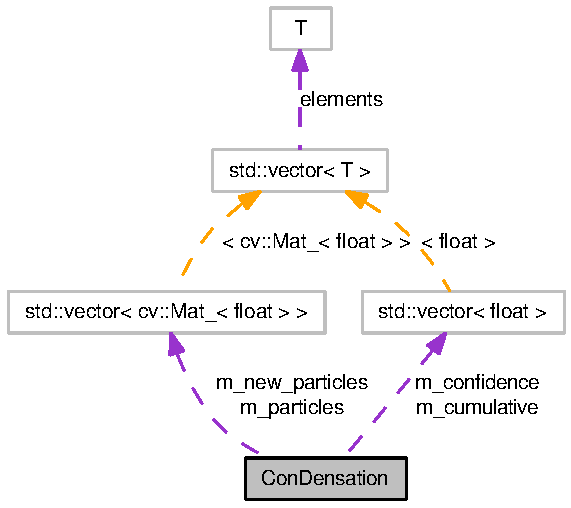
\includegraphics[width=302pt]{classConDensation__coll__graph}
\end{center}
\end{figure}
\subsection*{Public Member Functions}
\begin{DoxyCompactItemize}
\item 
\hyperlink{classConDensation_a3c7e76ac520287c7eb12bf3b05ad5fa0}{Con\-Densation} (unsigned int dynam\-\_\-params, unsigned int \hyperlink{social__robot_8cpp_acf574bc864f7f0fc111320f1d6c449d5}{num\-\_\-particles})
\item 
virtual \hyperlink{classConDensation_aa8176dc480168102bdd41ea10b977878}{$\sim$\-Con\-Densation} ()
\item 
void \hyperlink{classConDensation_aa61120a09e253fe429ee6a912f856fd5}{init\-\_\-sample\-\_\-set} (const float initial\mbox{[}$\,$\mbox{]}, const float std\-\_\-dev\mbox{[}$\,$\mbox{]})
\item 
void \hyperlink{classConDensation_a5aef436b8879d0e97b4503b609678740}{time\-\_\-update} ()
\end{DoxyCompactItemize}
\subsection*{Protected Attributes}
\begin{DoxyCompactItemize}
\item 
unsigned int \hyperlink{classConDensation_a19d27b83f57f5704c920a2ce0276639f}{m\-\_\-num\-\_\-states}
\item 
cv\-::\-Mat\-\_\-$<$ float $>$ \hyperlink{classConDensation_a4aef4dc8a1246b56ca4996cddb4ddebf}{m\-\_\-transition\-\_\-matrix}
\item 
cv\-::\-Mat\-\_\-$<$ float $>$ \hyperlink{classConDensation_ae50f5310d9c2b5574a7fe502b78f2ca1}{m\-\_\-state}
\item 
unsigned int \hyperlink{classConDensation_a6dd623ea8aa0fda252df3676dec562be}{m\-\_\-num\-\_\-particles}
\item 
std\-::vector$<$ cv\-::\-Mat\-\_\-$<$ float $>$ $>$ \hyperlink{classConDensation_a0500c90957d129d1f17512aa0ec4f490}{m\-\_\-particles}
\item 
std\-::vector$<$ float $>$ \hyperlink{classConDensation_abc5be0956acb4bd5c6383c4e095aac86}{m\-\_\-confidence}
\item 
std\-::vector$<$ cv\-::\-Mat\-\_\-$<$ float $>$ $>$ \hyperlink{classConDensation_a489443034896778939e5e24741d42728}{m\-\_\-new\-\_\-particles}
\item 
std\-::vector$<$ float $>$ \hyperlink{classConDensation_a9062fce705b93a2ab93c114aa579943a}{m\-\_\-cumulative}
\item 
cv\-::\-Mat\-\_\-$<$ float $>$ \hyperlink{classConDensation_a3908e7f2187a4b0010fadff24b950130}{m\-\_\-temp}
\item 
cv\-::\-R\-N\-G \hyperlink{classConDensation_a3485c3841850db0017d06781fa7064cf}{m\-\_\-rng}
\item 
const float $\ast$ \hyperlink{classConDensation_ace037712799e93339a0146a5f2891e35}{m\-\_\-std\-\_\-dev}
\end{DoxyCompactItemize}


\subsection{Detailed Description}
\begin{DoxyCopyright}{Copyright}

\end{DoxyCopyright}
Copyright 2012 Kevin Schluff

This program is free software\-: you can redistribute it and/or modify it under the terms of the G\-N\-U General Public License version 2, as published by the Free Software Foundation.

This program is distributed in the hope that it will be useful, but W\-I\-T\-H\-O\-U\-T A\-N\-Y W\-A\-R\-R\-A\-N\-T\-Y; without even the implied warranty of M\-E\-R\-C\-H\-A\-N\-T\-A\-B\-I\-L\-I\-T\-Y or F\-I\-T\-N\-E\-S\-S F\-O\-R A P\-A\-R\-T\-I\-C\-U\-L\-A\-R P\-U\-R\-P\-O\-S\-E. See the G\-N\-U General Public License for more details.

You should have received a copy of the G\-N\-U General Public License along with this program. If not, see \href{http://www.gnu.org/licenses/}{\tt http\-://www.\-gnu.\-org/licenses/}. 

\subsection{Constructor \& Destructor Documentation}
\hypertarget{classConDensation_a3c7e76ac520287c7eb12bf3b05ad5fa0}{\index{Con\-Densation@{Con\-Densation}!Con\-Densation@{Con\-Densation}}
\index{Con\-Densation@{Con\-Densation}!ConDensation@{Con\-Densation}}
\subsubsection[{Con\-Densation}]{\setlength{\rightskip}{0pt plus 5cm}Con\-Densation\-::\-Con\-Densation (
\begin{DoxyParamCaption}
\item[{unsigned int}]{dynam\-\_\-params, }
\item[{unsigned int}]{num\-\_\-particles}
\end{DoxyParamCaption}
)}}\label{classConDensation_a3c7e76ac520287c7eb12bf3b05ad5fa0}
\hypertarget{classConDensation_aa8176dc480168102bdd41ea10b977878}{\index{Con\-Densation@{Con\-Densation}!$\sim$\-Con\-Densation@{$\sim$\-Con\-Densation}}
\index{$\sim$\-Con\-Densation@{$\sim$\-Con\-Densation}!ConDensation@{Con\-Densation}}
\subsubsection[{$\sim$\-Con\-Densation}]{\setlength{\rightskip}{0pt plus 5cm}Con\-Densation\-::$\sim$\-Con\-Densation (
\begin{DoxyParamCaption}
{}
\end{DoxyParamCaption}
)\hspace{0.3cm}{\ttfamily [virtual]}}}\label{classConDensation_aa8176dc480168102bdd41ea10b977878}


\subsection{Member Function Documentation}
\hypertarget{classConDensation_aa61120a09e253fe429ee6a912f856fd5}{\index{Con\-Densation@{Con\-Densation}!init\-\_\-sample\-\_\-set@{init\-\_\-sample\-\_\-set}}
\index{init\-\_\-sample\-\_\-set@{init\-\_\-sample\-\_\-set}!ConDensation@{Con\-Densation}}
\subsubsection[{init\-\_\-sample\-\_\-set}]{\setlength{\rightskip}{0pt plus 5cm}void Con\-Densation\-::init\-\_\-sample\-\_\-set (
\begin{DoxyParamCaption}
\item[{const float}]{initial\mbox{[}$\,$\mbox{]}, }
\item[{const float}]{std\-\_\-dev\mbox{[}$\,$\mbox{]}}
\end{DoxyParamCaption}
)}}\label{classConDensation_aa61120a09e253fe429ee6a912f856fd5}
\hypertarget{classConDensation_a5aef436b8879d0e97b4503b609678740}{\index{Con\-Densation@{Con\-Densation}!time\-\_\-update@{time\-\_\-update}}
\index{time\-\_\-update@{time\-\_\-update}!ConDensation@{Con\-Densation}}
\subsubsection[{time\-\_\-update}]{\setlength{\rightskip}{0pt plus 5cm}void Con\-Densation\-::time\-\_\-update (
\begin{DoxyParamCaption}
{}
\end{DoxyParamCaption}
)}}\label{classConDensation_a5aef436b8879d0e97b4503b609678740}


\subsection{Field Documentation}
\hypertarget{classConDensation_abc5be0956acb4bd5c6383c4e095aac86}{\index{Con\-Densation@{Con\-Densation}!m\-\_\-confidence@{m\-\_\-confidence}}
\index{m\-\_\-confidence@{m\-\_\-confidence}!ConDensation@{Con\-Densation}}
\subsubsection[{m\-\_\-confidence}]{\setlength{\rightskip}{0pt plus 5cm}std\-::vector$<$float$>$ Con\-Densation\-::m\-\_\-confidence\hspace{0.3cm}{\ttfamily [protected]}}}\label{classConDensation_abc5be0956acb4bd5c6383c4e095aac86}
\hypertarget{classConDensation_a9062fce705b93a2ab93c114aa579943a}{\index{Con\-Densation@{Con\-Densation}!m\-\_\-cumulative@{m\-\_\-cumulative}}
\index{m\-\_\-cumulative@{m\-\_\-cumulative}!ConDensation@{Con\-Densation}}
\subsubsection[{m\-\_\-cumulative}]{\setlength{\rightskip}{0pt plus 5cm}std\-::vector$<$float$>$ Con\-Densation\-::m\-\_\-cumulative\hspace{0.3cm}{\ttfamily [protected]}}}\label{classConDensation_a9062fce705b93a2ab93c114aa579943a}
\hypertarget{classConDensation_a489443034896778939e5e24741d42728}{\index{Con\-Densation@{Con\-Densation}!m\-\_\-new\-\_\-particles@{m\-\_\-new\-\_\-particles}}
\index{m\-\_\-new\-\_\-particles@{m\-\_\-new\-\_\-particles}!ConDensation@{Con\-Densation}}
\subsubsection[{m\-\_\-new\-\_\-particles}]{\setlength{\rightskip}{0pt plus 5cm}std\-::vector$<$cv\-::\-Mat\-\_\-$<$float$>$ $>$ Con\-Densation\-::m\-\_\-new\-\_\-particles\hspace{0.3cm}{\ttfamily [protected]}}}\label{classConDensation_a489443034896778939e5e24741d42728}
\hypertarget{classConDensation_a6dd623ea8aa0fda252df3676dec562be}{\index{Con\-Densation@{Con\-Densation}!m\-\_\-num\-\_\-particles@{m\-\_\-num\-\_\-particles}}
\index{m\-\_\-num\-\_\-particles@{m\-\_\-num\-\_\-particles}!ConDensation@{Con\-Densation}}
\subsubsection[{m\-\_\-num\-\_\-particles}]{\setlength{\rightskip}{0pt plus 5cm}unsigned int Con\-Densation\-::m\-\_\-num\-\_\-particles\hspace{0.3cm}{\ttfamily [protected]}}}\label{classConDensation_a6dd623ea8aa0fda252df3676dec562be}
\hypertarget{classConDensation_a19d27b83f57f5704c920a2ce0276639f}{\index{Con\-Densation@{Con\-Densation}!m\-\_\-num\-\_\-states@{m\-\_\-num\-\_\-states}}
\index{m\-\_\-num\-\_\-states@{m\-\_\-num\-\_\-states}!ConDensation@{Con\-Densation}}
\subsubsection[{m\-\_\-num\-\_\-states}]{\setlength{\rightskip}{0pt plus 5cm}unsigned int Con\-Densation\-::m\-\_\-num\-\_\-states\hspace{0.3cm}{\ttfamily [protected]}}}\label{classConDensation_a19d27b83f57f5704c920a2ce0276639f}
\hypertarget{classConDensation_a0500c90957d129d1f17512aa0ec4f490}{\index{Con\-Densation@{Con\-Densation}!m\-\_\-particles@{m\-\_\-particles}}
\index{m\-\_\-particles@{m\-\_\-particles}!ConDensation@{Con\-Densation}}
\subsubsection[{m\-\_\-particles}]{\setlength{\rightskip}{0pt plus 5cm}std\-::vector$<$cv\-::\-Mat\-\_\-$<$float$>$ $>$ Con\-Densation\-::m\-\_\-particles\hspace{0.3cm}{\ttfamily [protected]}}}\label{classConDensation_a0500c90957d129d1f17512aa0ec4f490}
\hypertarget{classConDensation_a3485c3841850db0017d06781fa7064cf}{\index{Con\-Densation@{Con\-Densation}!m\-\_\-rng@{m\-\_\-rng}}
\index{m\-\_\-rng@{m\-\_\-rng}!ConDensation@{Con\-Densation}}
\subsubsection[{m\-\_\-rng}]{\setlength{\rightskip}{0pt plus 5cm}cv\-::\-R\-N\-G Con\-Densation\-::m\-\_\-rng\hspace{0.3cm}{\ttfamily [protected]}}}\label{classConDensation_a3485c3841850db0017d06781fa7064cf}
\hypertarget{classConDensation_ae50f5310d9c2b5574a7fe502b78f2ca1}{\index{Con\-Densation@{Con\-Densation}!m\-\_\-state@{m\-\_\-state}}
\index{m\-\_\-state@{m\-\_\-state}!ConDensation@{Con\-Densation}}
\subsubsection[{m\-\_\-state}]{\setlength{\rightskip}{0pt plus 5cm}cv\-::\-Mat\-\_\-$<$float$>$ Con\-Densation\-::m\-\_\-state\hspace{0.3cm}{\ttfamily [protected]}}}\label{classConDensation_ae50f5310d9c2b5574a7fe502b78f2ca1}
\hypertarget{classConDensation_ace037712799e93339a0146a5f2891e35}{\index{Con\-Densation@{Con\-Densation}!m\-\_\-std\-\_\-dev@{m\-\_\-std\-\_\-dev}}
\index{m\-\_\-std\-\_\-dev@{m\-\_\-std\-\_\-dev}!ConDensation@{Con\-Densation}}
\subsubsection[{m\-\_\-std\-\_\-dev}]{\setlength{\rightskip}{0pt plus 5cm}const float$\ast$ Con\-Densation\-::m\-\_\-std\-\_\-dev\hspace{0.3cm}{\ttfamily [protected]}}}\label{classConDensation_ace037712799e93339a0146a5f2891e35}
\hypertarget{classConDensation_a3908e7f2187a4b0010fadff24b950130}{\index{Con\-Densation@{Con\-Densation}!m\-\_\-temp@{m\-\_\-temp}}
\index{m\-\_\-temp@{m\-\_\-temp}!ConDensation@{Con\-Densation}}
\subsubsection[{m\-\_\-temp}]{\setlength{\rightskip}{0pt plus 5cm}cv\-::\-Mat\-\_\-$<$float$>$ Con\-Densation\-::m\-\_\-temp\hspace{0.3cm}{\ttfamily [protected]}}}\label{classConDensation_a3908e7f2187a4b0010fadff24b950130}
\hypertarget{classConDensation_a4aef4dc8a1246b56ca4996cddb4ddebf}{\index{Con\-Densation@{Con\-Densation}!m\-\_\-transition\-\_\-matrix@{m\-\_\-transition\-\_\-matrix}}
\index{m\-\_\-transition\-\_\-matrix@{m\-\_\-transition\-\_\-matrix}!ConDensation@{Con\-Densation}}
\subsubsection[{m\-\_\-transition\-\_\-matrix}]{\setlength{\rightskip}{0pt plus 5cm}cv\-::\-Mat\-\_\-$<$float$>$ Con\-Densation\-::m\-\_\-transition\-\_\-matrix\hspace{0.3cm}{\ttfamily [protected]}}}\label{classConDensation_a4aef4dc8a1246b56ca4996cddb4ddebf}


The documentation for this class was generated from the following files\-:\begin{DoxyCompactItemize}
\item 
\hyperlink{condens_8h}{condens.\-h}\item 
\hyperlink{condens_8cpp}{condens.\-cpp}\end{DoxyCompactItemize}

\hypertarget{classCvBar}{
\section{CvBar Class Reference}
\label{classCvBar}\index{CvBar@{CvBar}}
}


{\ttfamily \#include $<$window\_\-QT.h$>$}



Inheritance diagram for CvBar:\nopagebreak
\begin{figure}[H]
\begin{center}
\leavevmode
\includegraphics[width=194pt]{classCvBar__inherit__graph}
\end{center}
\end{figure}
\subsection*{Data Fields}
\begin{DoxyCompactItemize}
\item 
\hyperlink{window__QT_8h_a4003d2816fd898b0f71eb5addfe80af3}{typeBar} \hyperlink{classCvBar_a64329aa3255c2c98a36f3f887a939b40}{type}
\item 
QString \hyperlink{classCvBar_a6970f0eae76786143e2df415681d0a6f}{name\_\-bar}
\item 
QPointer$<$ QWidget $>$ \hyperlink{classCvBar_af6fa35b8c9f4aed557854fc3aa80a040}{myparent}
\end{DoxyCompactItemize}


\subsection{Field Documentation}
\hypertarget{classCvBar_af6fa35b8c9f4aed557854fc3aa80a040}{
\index{CvBar@{CvBar}!myparent@{myparent}}
\index{myparent@{myparent}!CvBar@{CvBar}}
\subsubsection[{myparent}]{\setlength{\rightskip}{0pt plus 5cm}QPointer$<$QWidget$>$ {\bf CvBar::myparent}}}
\label{classCvBar_af6fa35b8c9f4aed557854fc3aa80a040}
\hypertarget{classCvBar_a6970f0eae76786143e2df415681d0a6f}{
\index{CvBar@{CvBar}!name\_\-bar@{name\_\-bar}}
\index{name\_\-bar@{name\_\-bar}!CvBar@{CvBar}}
\subsubsection[{name\_\-bar}]{\setlength{\rightskip}{0pt plus 5cm}QString {\bf CvBar::name\_\-bar}}}
\label{classCvBar_a6970f0eae76786143e2df415681d0a6f}
\hypertarget{classCvBar_a64329aa3255c2c98a36f3f887a939b40}{
\index{CvBar@{CvBar}!type@{type}}
\index{type@{type}!CvBar@{CvBar}}
\subsubsection[{type}]{\setlength{\rightskip}{0pt plus 5cm}{\bf typeBar} {\bf CvBar::type}}}
\label{classCvBar_a64329aa3255c2c98a36f3f887a939b40}


The documentation for this class was generated from the following file:\begin{DoxyCompactItemize}
\item 
\hyperlink{window__QT_8h}{window\_\-QT.h}\end{DoxyCompactItemize}

\hypertarget{classCvButtonbar}{
\section{CvButtonbar Class Reference}
\label{classCvButtonbar}\index{CvButtonbar@{CvButtonbar}}
}


{\ttfamily \#include $<$window\_\-QT.h$>$}



Inheritance diagram for CvButtonbar:\nopagebreak
\begin{figure}[H]
\begin{center}
\leavevmode
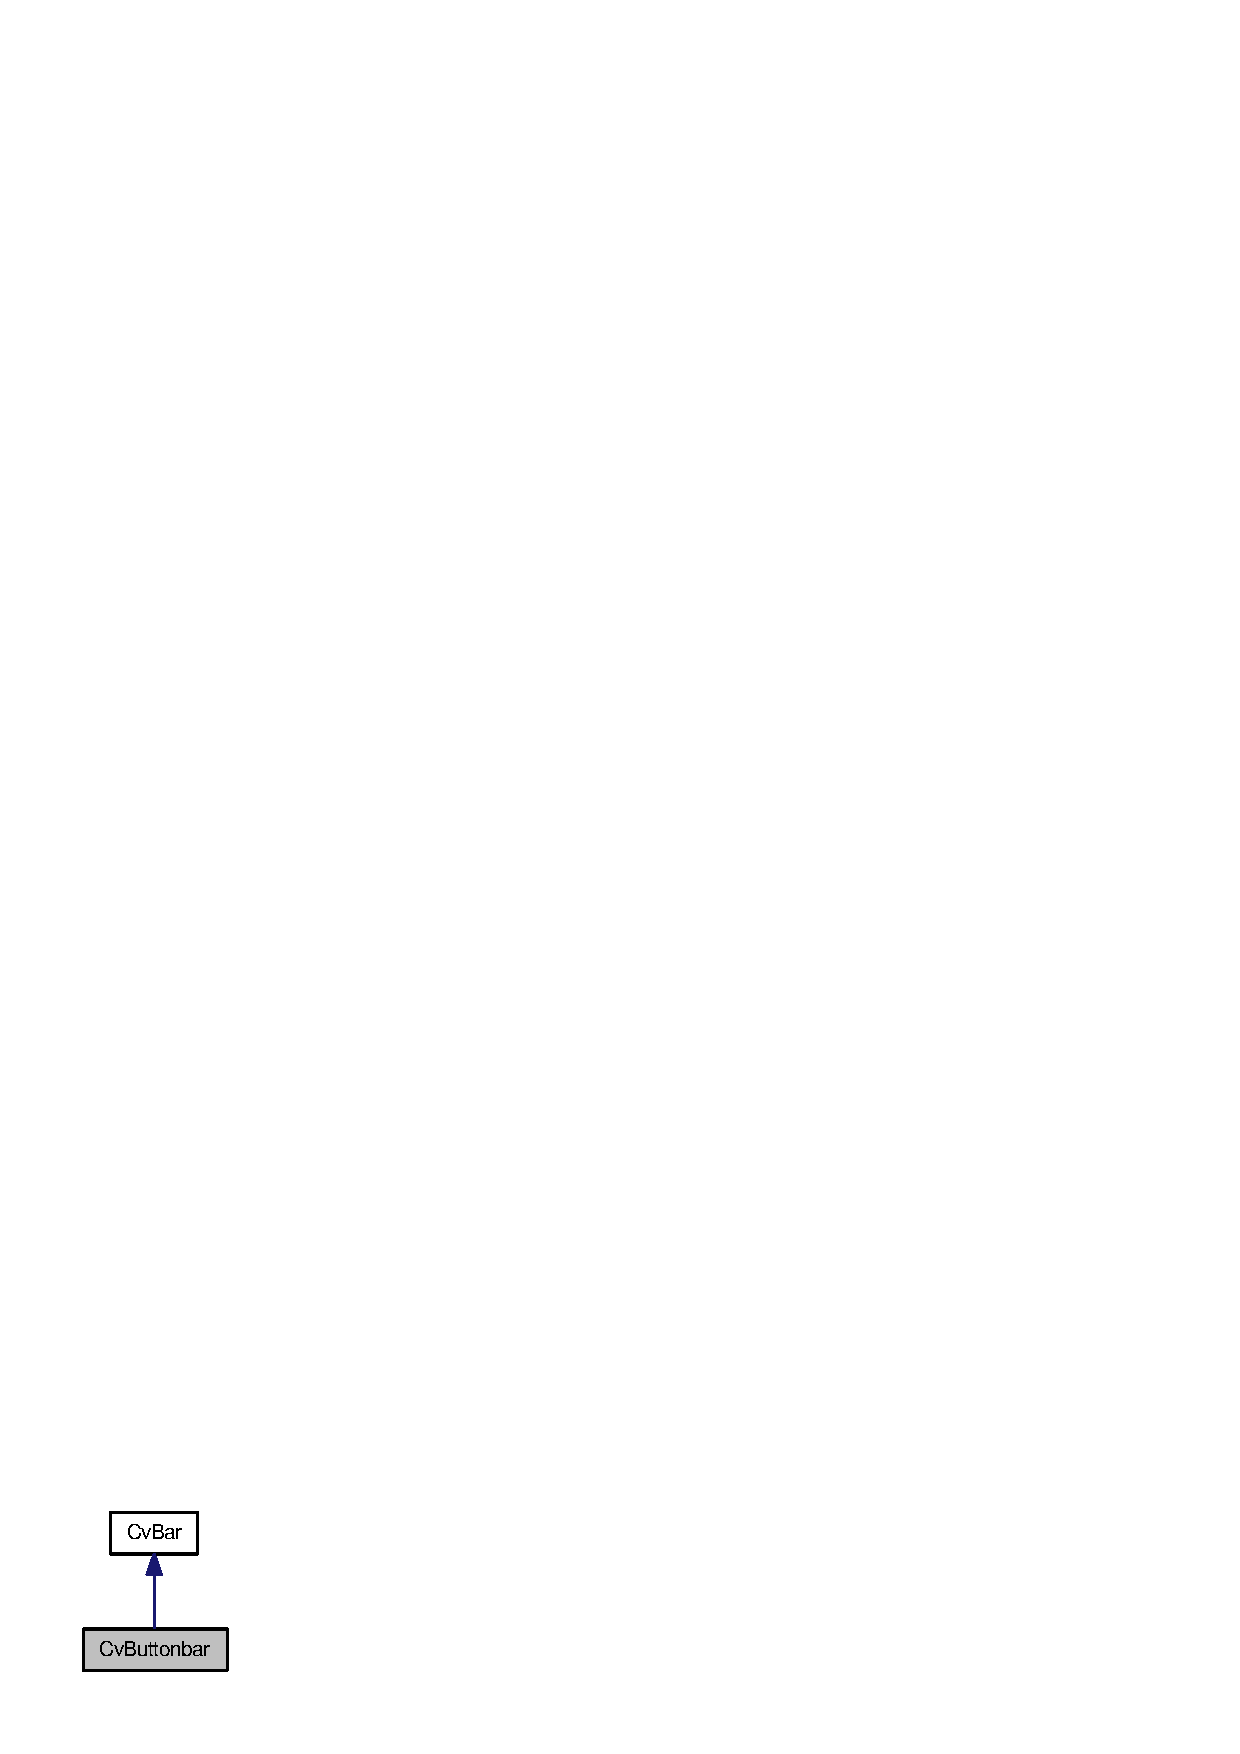
\includegraphics[width=112pt]{classCvButtonbar__inherit__graph}
\end{center}
\end{figure}


Collaboration diagram for CvButtonbar:\nopagebreak
\begin{figure}[H]
\begin{center}
\leavevmode
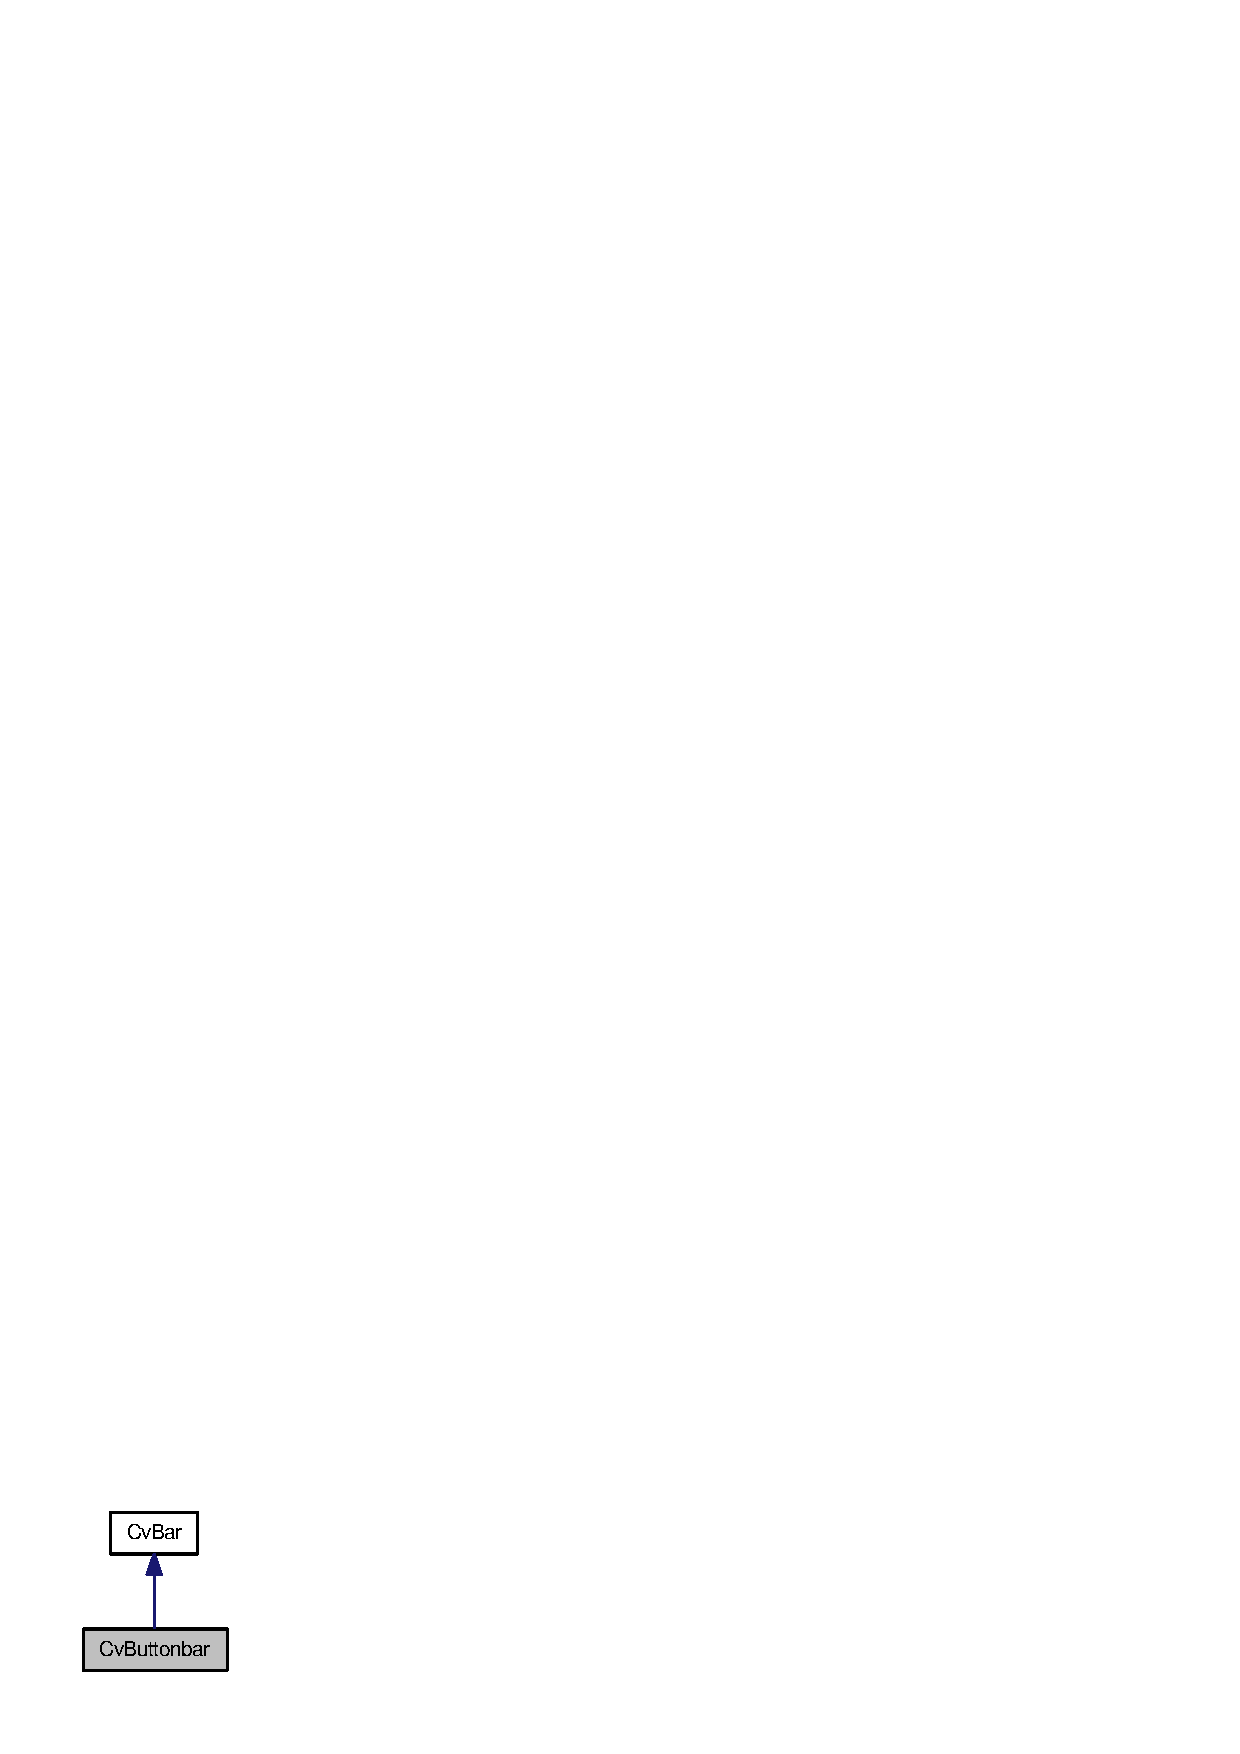
\includegraphics[width=112pt]{classCvButtonbar__coll__graph}
\end{center}
\end{figure}
\subsection*{Public Member Functions}
\begin{DoxyCompactItemize}
\item 
\hyperlink{classCvButtonbar_a2e242a93211a0ce57be59c9558c61487}{CvButtonbar} (QWidget $\ast$arg, QString bar\_\-name)
\item 
\hyperlink{classCvButtonbar_a53d7f1aa214a6f8b31b9e69c8806f49f}{$\sim$CvButtonbar} ()
\item 
void \hyperlink{classCvButtonbar_a9d85c6030793e2abeab43e300ed81687}{addButton} (QString button\_\-name, CvButtonCallback call, void $\ast$userdata, int button\_\-type, int initial\_\-button\_\-state)
\end{DoxyCompactItemize}


\subsection{Constructor \& Destructor Documentation}
\hypertarget{classCvButtonbar_a2e242a93211a0ce57be59c9558c61487}{
\index{CvButtonbar@{CvButtonbar}!CvButtonbar@{CvButtonbar}}
\index{CvButtonbar@{CvButtonbar}!CvButtonbar@{CvButtonbar}}
\subsubsection[{CvButtonbar}]{\setlength{\rightskip}{0pt plus 5cm}CvButtonbar::CvButtonbar (QWidget $\ast$ {\em arg}, \/  QString {\em bar\_\-name})}}
\label{classCvButtonbar_a2e242a93211a0ce57be59c9558c61487}
\hypertarget{classCvButtonbar_a53d7f1aa214a6f8b31b9e69c8806f49f}{
\index{CvButtonbar@{CvButtonbar}!$\sim$CvButtonbar@{$\sim$CvButtonbar}}
\index{$\sim$CvButtonbar@{$\sim$CvButtonbar}!CvButtonbar@{CvButtonbar}}
\subsubsection[{$\sim$CvButtonbar}]{\setlength{\rightskip}{0pt plus 5cm}CvButtonbar::$\sim$CvButtonbar ()}}
\label{classCvButtonbar_a53d7f1aa214a6f8b31b9e69c8806f49f}


\subsection{Member Function Documentation}
\hypertarget{classCvButtonbar_a9d85c6030793e2abeab43e300ed81687}{
\index{CvButtonbar@{CvButtonbar}!addButton@{addButton}}
\index{addButton@{addButton}!CvButtonbar@{CvButtonbar}}
\subsubsection[{addButton}]{\setlength{\rightskip}{0pt plus 5cm}void CvButtonbar::addButton (QString {\em button\_\-name}, \/  CvButtonCallback {\em call}, \/  void $\ast$ {\em userdata}, \/  int {\em button\_\-type}, \/  int {\em initial\_\-button\_\-state})}}
\label{classCvButtonbar_a9d85c6030793e2abeab43e300ed81687}


The documentation for this class was generated from the following files:\begin{DoxyCompactItemize}
\item 
\hyperlink{window__QT_8h}{window\_\-QT.h}\item 
\hyperlink{window__QT_8cpp}{window\_\-QT.cpp}\end{DoxyCompactItemize}

\hypertarget{classCvCheckBox}{\section{Cv\-Check\-Box Class Reference}
\label{classCvCheckBox}\index{Cv\-Check\-Box@{Cv\-Check\-Box}}
}


{\ttfamily \#include $<$window\-\_\-\-Q\-T.\-h$>$}



Inheritance diagram for Cv\-Check\-Box\-:\nopagebreak
\begin{figure}[H]
\begin{center}
\leavevmode
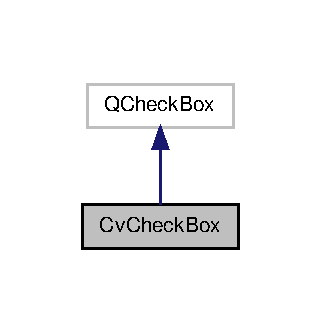
\includegraphics[width=154pt]{classCvCheckBox__inherit__graph}
\end{center}
\end{figure}


Collaboration diagram for Cv\-Check\-Box\-:\nopagebreak
\begin{figure}[H]
\begin{center}
\leavevmode
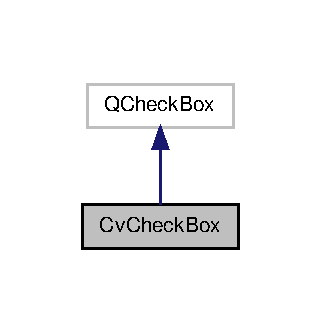
\includegraphics[width=154pt]{classCvCheckBox__coll__graph}
\end{center}
\end{figure}
\subsection*{Public Member Functions}
\begin{DoxyCompactItemize}
\item 
\hyperlink{classCvCheckBox_ad281545b29a827077ab4f4a4349bf582}{Cv\-Check\-Box} (\hyperlink{classCvButtonbar}{Cv\-Buttonbar} $\ast$par, Q\-String button\-\_\-name, Cv\-Button\-Callback call, void $\ast$userdata, int initial\-\_\-button\-\_\-state)
\end{DoxyCompactItemize}


\subsection{Constructor \& Destructor Documentation}
\hypertarget{classCvCheckBox_ad281545b29a827077ab4f4a4349bf582}{\index{Cv\-Check\-Box@{Cv\-Check\-Box}!Cv\-Check\-Box@{Cv\-Check\-Box}}
\index{Cv\-Check\-Box@{Cv\-Check\-Box}!CvCheckBox@{Cv\-Check\-Box}}
\subsubsection[{Cv\-Check\-Box}]{\setlength{\rightskip}{0pt plus 5cm}Cv\-Check\-Box\-::\-Cv\-Check\-Box (
\begin{DoxyParamCaption}
\item[{{\bf Cv\-Buttonbar} $\ast$}]{par, }
\item[{Q\-String}]{button\-\_\-name, }
\item[{Cv\-Button\-Callback}]{call, }
\item[{void $\ast$}]{userdata, }
\item[{int}]{initial\-\_\-button\-\_\-state}
\end{DoxyParamCaption}
)}}\label{classCvCheckBox_ad281545b29a827077ab4f4a4349bf582}


The documentation for this class was generated from the following files\-:\begin{DoxyCompactItemize}
\item 
\hyperlink{window__QT_8h}{window\-\_\-\-Q\-T.\-h}\item 
\hyperlink{window__QT_8cpp}{window\-\_\-\-Q\-T.\-cpp}\end{DoxyCompactItemize}

\hypertarget{classCvPushButton}{\section{Cv\-Push\-Button Class Reference}
\label{classCvPushButton}\index{Cv\-Push\-Button@{Cv\-Push\-Button}}
}


{\ttfamily \#include $<$window\-\_\-\-Q\-T.\-h$>$}



Inheritance diagram for Cv\-Push\-Button\-:
\nopagebreak
\begin{figure}[H]
\begin{center}
\leavevmode
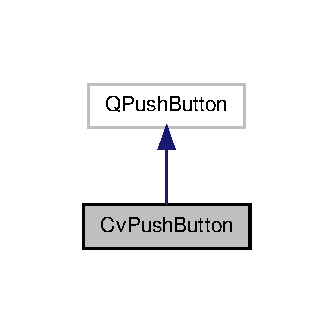
\includegraphics[width=160pt]{classCvPushButton__inherit__graph}
\end{center}
\end{figure}


Collaboration diagram for Cv\-Push\-Button\-:
\nopagebreak
\begin{figure}[H]
\begin{center}
\leavevmode
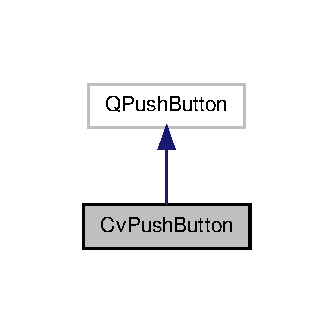
\includegraphics[width=160pt]{classCvPushButton__coll__graph}
\end{center}
\end{figure}
\subsection*{Public Member Functions}
\begin{DoxyCompactItemize}
\item 
\hyperlink{classCvPushButton_add13c78f22d066ca5dc5a598102890da}{Cv\-Push\-Button} (\hyperlink{classCvButtonbar}{Cv\-Buttonbar} $\ast$par, Q\-String button\-\_\-name, Cv\-Button\-Callback call, void $\ast$userdata)
\end{DoxyCompactItemize}


\subsection{Constructor \& Destructor Documentation}
\hypertarget{classCvPushButton_add13c78f22d066ca5dc5a598102890da}{\index{Cv\-Push\-Button@{Cv\-Push\-Button}!Cv\-Push\-Button@{Cv\-Push\-Button}}
\index{Cv\-Push\-Button@{Cv\-Push\-Button}!CvPushButton@{Cv\-Push\-Button}}
\subsubsection[{Cv\-Push\-Button}]{\setlength{\rightskip}{0pt plus 5cm}Cv\-Push\-Button\-::\-Cv\-Push\-Button (
\begin{DoxyParamCaption}
\item[{{\bf Cv\-Buttonbar} $\ast$}]{par, }
\item[{Q\-String}]{button\-\_\-name, }
\item[{Cv\-Button\-Callback}]{call, }
\item[{void $\ast$}]{userdata}
\end{DoxyParamCaption}
)}}\label{classCvPushButton_add13c78f22d066ca5dc5a598102890da}


The documentation for this class was generated from the following files\-:\begin{DoxyCompactItemize}
\item 
\hyperlink{window__QT_8h}{window\-\_\-\-Q\-T.\-h}\item 
\hyperlink{window__QT_8cpp}{window\-\_\-\-Q\-T.\-cpp}\end{DoxyCompactItemize}

\hypertarget{classCvRadioButton}{\section{Cv\-Radio\-Button Class Reference}
\label{classCvRadioButton}\index{Cv\-Radio\-Button@{Cv\-Radio\-Button}}
}


{\ttfamily \#include $<$window\-\_\-\-Q\-T.\-h$>$}



Inheritance diagram for Cv\-Radio\-Button\-:
\nopagebreak
\begin{figure}[H]
\begin{center}
\leavevmode
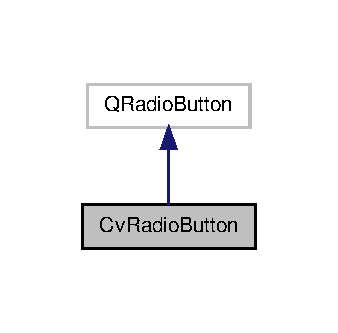
\includegraphics[width=162pt]{classCvRadioButton__inherit__graph}
\end{center}
\end{figure}


Collaboration diagram for Cv\-Radio\-Button\-:
\nopagebreak
\begin{figure}[H]
\begin{center}
\leavevmode
\includegraphics[width=162pt]{classCvRadioButton__coll__graph}
\end{center}
\end{figure}
\subsection*{Public Member Functions}
\begin{DoxyCompactItemize}
\item 
\hyperlink{classCvRadioButton_ac083eb56a708d7c70d12392b3c6bb1ba}{Cv\-Radio\-Button} (\hyperlink{classCvButtonbar}{Cv\-Buttonbar} $\ast$par, Q\-String button\-\_\-name, Cv\-Button\-Callback call, void $\ast$userdata, int initial\-\_\-button\-\_\-state)
\end{DoxyCompactItemize}


\subsection{Constructor \& Destructor Documentation}
\hypertarget{classCvRadioButton_ac083eb56a708d7c70d12392b3c6bb1ba}{\index{Cv\-Radio\-Button@{Cv\-Radio\-Button}!Cv\-Radio\-Button@{Cv\-Radio\-Button}}
\index{Cv\-Radio\-Button@{Cv\-Radio\-Button}!CvRadioButton@{Cv\-Radio\-Button}}
\subsubsection[{Cv\-Radio\-Button}]{\setlength{\rightskip}{0pt plus 5cm}Cv\-Radio\-Button\-::\-Cv\-Radio\-Button (
\begin{DoxyParamCaption}
\item[{{\bf Cv\-Buttonbar} $\ast$}]{par, }
\item[{Q\-String}]{button\-\_\-name, }
\item[{Cv\-Button\-Callback}]{call, }
\item[{void $\ast$}]{userdata, }
\item[{int}]{initial\-\_\-button\-\_\-state}
\end{DoxyParamCaption}
)}}\label{classCvRadioButton_ac083eb56a708d7c70d12392b3c6bb1ba}


The documentation for this class was generated from the following files\-:\begin{DoxyCompactItemize}
\item 
\hyperlink{window__QT_8h}{window\-\_\-\-Q\-T.\-h}\item 
\hyperlink{window__QT_8cpp}{window\-\_\-\-Q\-T.\-cpp}\end{DoxyCompactItemize}

\hypertarget{classCvTrackbar}{\section{Cv\-Trackbar Class Reference}
\label{classCvTrackbar}\index{Cv\-Trackbar@{Cv\-Trackbar}}
}


{\ttfamily \#include $<$window\-\_\-\-Q\-T.\-h$>$}



Inheritance diagram for Cv\-Trackbar\-:
\nopagebreak
\begin{figure}[H]
\begin{center}
\leavevmode
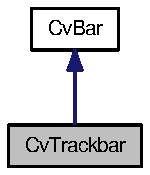
\includegraphics[width=158pt]{classCvTrackbar__inherit__graph}
\end{center}
\end{figure}


Collaboration diagram for Cv\-Trackbar\-:
\nopagebreak
\begin{figure}[H]
\begin{center}
\leavevmode
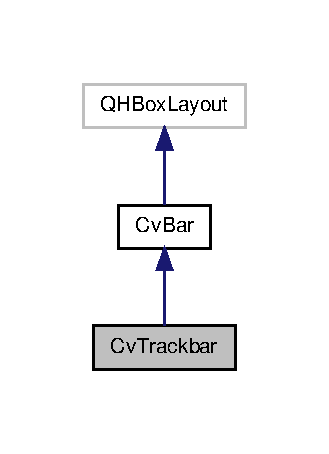
\includegraphics[width=158pt]{classCvTrackbar__coll__graph}
\end{center}
\end{figure}
\subsection*{Public Member Functions}
\begin{DoxyCompactItemize}
\item 
\hyperlink{classCvTrackbar_a5666e87ce86ec7ad97d62b89d148e9bb}{Cv\-Trackbar} (\hyperlink{classCvWindow}{Cv\-Window} $\ast$parent, Q\-String name, int $\ast$value, int count, Cv\-Trackbar\-Callback on\-\_\-change)
\item 
\hyperlink{classCvTrackbar_a36624a0a15c46a3320ce29f20eda8db8}{Cv\-Trackbar} (\hyperlink{classCvWindow}{Cv\-Window} $\ast$parent, Q\-String name, int $\ast$value, int count, Cv\-Trackbar\-Callback2 on\-\_\-change, void $\ast$data)
\item 
\hyperlink{classCvTrackbar_ae9bcf438807648149bc24d64d9294ac9}{$\sim$\-Cv\-Trackbar} ()
\end{DoxyCompactItemize}
\subsection*{Data Fields}
\begin{DoxyCompactItemize}
\item 
Q\-Pointer$<$ Q\-Slider $>$ \hyperlink{classCvTrackbar_afc7525a204cd578c21b23b842cbe28d8}{slider}
\end{DoxyCompactItemize}


\subsection{Constructor \& Destructor Documentation}
\hypertarget{classCvTrackbar_a5666e87ce86ec7ad97d62b89d148e9bb}{\index{Cv\-Trackbar@{Cv\-Trackbar}!Cv\-Trackbar@{Cv\-Trackbar}}
\index{Cv\-Trackbar@{Cv\-Trackbar}!CvTrackbar@{Cv\-Trackbar}}
\subsubsection[{Cv\-Trackbar}]{\setlength{\rightskip}{0pt plus 5cm}Cv\-Trackbar\-::\-Cv\-Trackbar (
\begin{DoxyParamCaption}
\item[{{\bf Cv\-Window} $\ast$}]{parent, }
\item[{Q\-String}]{name, }
\item[{int $\ast$}]{value, }
\item[{int}]{count, }
\item[{Cv\-Trackbar\-Callback}]{on\-\_\-change}
\end{DoxyParamCaption}
)}}\label{classCvTrackbar_a5666e87ce86ec7ad97d62b89d148e9bb}
\hypertarget{classCvTrackbar_a36624a0a15c46a3320ce29f20eda8db8}{\index{Cv\-Trackbar@{Cv\-Trackbar}!Cv\-Trackbar@{Cv\-Trackbar}}
\index{Cv\-Trackbar@{Cv\-Trackbar}!CvTrackbar@{Cv\-Trackbar}}
\subsubsection[{Cv\-Trackbar}]{\setlength{\rightskip}{0pt plus 5cm}Cv\-Trackbar\-::\-Cv\-Trackbar (
\begin{DoxyParamCaption}
\item[{{\bf Cv\-Window} $\ast$}]{parent, }
\item[{Q\-String}]{name, }
\item[{int $\ast$}]{value, }
\item[{int}]{count, }
\item[{Cv\-Trackbar\-Callback2}]{on\-\_\-change, }
\item[{void $\ast$}]{data}
\end{DoxyParamCaption}
)}}\label{classCvTrackbar_a36624a0a15c46a3320ce29f20eda8db8}
\hypertarget{classCvTrackbar_ae9bcf438807648149bc24d64d9294ac9}{\index{Cv\-Trackbar@{Cv\-Trackbar}!$\sim$\-Cv\-Trackbar@{$\sim$\-Cv\-Trackbar}}
\index{$\sim$\-Cv\-Trackbar@{$\sim$\-Cv\-Trackbar}!CvTrackbar@{Cv\-Trackbar}}
\subsubsection[{$\sim$\-Cv\-Trackbar}]{\setlength{\rightskip}{0pt plus 5cm}Cv\-Trackbar\-::$\sim$\-Cv\-Trackbar (
\begin{DoxyParamCaption}
{}
\end{DoxyParamCaption}
)}}\label{classCvTrackbar_ae9bcf438807648149bc24d64d9294ac9}


\subsection{Field Documentation}
\hypertarget{classCvTrackbar_afc7525a204cd578c21b23b842cbe28d8}{\index{Cv\-Trackbar@{Cv\-Trackbar}!slider@{slider}}
\index{slider@{slider}!CvTrackbar@{Cv\-Trackbar}}
\subsubsection[{slider}]{\setlength{\rightskip}{0pt plus 5cm}Q\-Pointer$<$Q\-Slider$>$ Cv\-Trackbar\-::slider}}\label{classCvTrackbar_afc7525a204cd578c21b23b842cbe28d8}


The documentation for this class was generated from the following files\-:\begin{DoxyCompactItemize}
\item 
\hyperlink{window__QT_8h}{window\-\_\-\-Q\-T.\-h}\item 
\hyperlink{window__QT_8cpp}{window\-\_\-\-Q\-T.\-cpp}\end{DoxyCompactItemize}

\hypertarget{classCvUtils}{\section{Cv\-Utils Class Reference}
\label{classCvUtils}\index{Cv\-Utils@{Cv\-Utils}}
}


This class contains useful functions for the image processing part.  




{\ttfamily \#include $<$Cv\-Utils.\-h$>$}

\subsection*{Public Member Functions}
\begin{DoxyCompactItemize}
\item 
Mat \hyperlink{classCvUtils_aa5bded11699d39af25c420aed2ade0ba}{rgb2bw} (Mat im\-\_\-rgb)
\item 
Mat \hyperlink{classCvUtils_a47189479acb67a1918f35557fc5906a6}{preprocessing} (Mat \hyperlink{createGT_8cpp_aabb27b8973575043030df51be47cd24a}{image})
\item 
void \hyperlink{classCvUtils_a426439fc003e5557644932eee66c48b6}{get\-\_\-non\-\_\-zeros} (Mat img, Mat prob, vector$<$ Point3f $>$ $\ast$points, Point pdiff=Point(0, 0), double scale=1)
\end{DoxyCompactItemize}
\begin{Indent}{\bf Drawing functions}\par
\begin{DoxyCompactItemize}
\item 
void \hyperlink{classCvUtils_a74249b2e9b76b2a8ae2c01c4ff496663}{draw\-\_\-rgb\-\_\-faces} (Mat \&img, vector$<$ Rect $>$ faces)
\item 
void \hyperlink{classCvUtils_ac86c2ad8adca706655831938b63ebaa2}{draw\-\_\-tracking\-\_\-faces} (Mat \&img, vector$<$ \hyperlink{classStateData}{State\-Data} $>$ \hyperlink{social__robot_8cpp_a63ba5e41659a1483954bc6564bca605a}{state\-\_\-datas})
\item 
void \hyperlink{classCvUtils_a6e1f3369c2b553c06f2692c75e20667d}{draw\-\_\-depth\-\_\-faces} (Mat \&img, vector$<$ Rect $>$ faces)
\end{DoxyCompactItemize}
\end{Indent}
\begin{Indent}{\bf Get the center of a rectangle}\par
\begin{DoxyCompactItemize}
\item 
Point \hyperlink{classCvUtils_aa54494728db8503a7311ff2f9ad8ab1c}{get\-\_\-rect\-\_\-centre} (Rect rect)
\item 
Point3f \hyperlink{classCvUtils_a9a91a1dbd7a74ef15257510129308277}{get\-\_\-rect\-\_\-centre\-\_\-3d} (Rect rect, Mat \hyperlink{social__robot__onethread_8cpp_a5b613972ff73fd7b34e0ee18acc5c1a6}{depth\-\_\-image})
\end{DoxyCompactItemize}
\end{Indent}
\begin{Indent}{\bf Euclidean Distance}\par
\begin{DoxyCompactItemize}
\item 
double \hyperlink{classCvUtils_a20d53b92663d548bebf90da242d984f3}{euclidean\-\_\-distance} (Point3f a, Point3f b)
\item 
double \hyperlink{classCvUtils_a74b4a32b47136f704db2729b39095c02}{euclidean\-\_\-distance} (Point a, Point b)
\item 
Rect \hyperlink{classCvUtils_a349894b926e2d252d0ce224abcba698a}{enlarge\-\_\-window} (Rect orgrect, Mat \hyperlink{createGT_8cpp_aabb27b8973575043030df51be47cd24a}{image}, double scale=2.\-0)
\end{DoxyCompactItemize}
\end{Indent}


\subsection{Detailed Description}
This class contains useful functions for the image processing part. 

\begin{DoxyAuthor}{Author}
Social Robot 
\end{DoxyAuthor}


\subsection{Member Function Documentation}
\hypertarget{classCvUtils_a6e1f3369c2b553c06f2692c75e20667d}{\index{Cv\-Utils@{Cv\-Utils}!draw\-\_\-depth\-\_\-faces@{draw\-\_\-depth\-\_\-faces}}
\index{draw\-\_\-depth\-\_\-faces@{draw\-\_\-depth\-\_\-faces}!CvUtils@{Cv\-Utils}}
\subsubsection[{draw\-\_\-depth\-\_\-faces}]{\setlength{\rightskip}{0pt plus 5cm}void Cv\-Utils\-::draw\-\_\-depth\-\_\-faces (
\begin{DoxyParamCaption}
\item[{Mat \&}]{img, }
\item[{vector$<$ Rect $>$}]{faces}
\end{DoxyParamCaption}
)}}\label{classCvUtils_a6e1f3369c2b553c06f2692c75e20667d}
This function draws the rectangles given in a vector in a depth image. \begin{DoxyReturn}{Returns}
void 
\end{DoxyReturn}

\begin{DoxyParams}{Parameters}
{\em \&img} & A Mat containing an image. \\
\hline
{\em faces} & A vector$<$\-Rect$>$ that contains the rectangles bounding the faces. \\
\hline
\end{DoxyParams}
\hypertarget{classCvUtils_a74249b2e9b76b2a8ae2c01c4ff496663}{\index{Cv\-Utils@{Cv\-Utils}!draw\-\_\-rgb\-\_\-faces@{draw\-\_\-rgb\-\_\-faces}}
\index{draw\-\_\-rgb\-\_\-faces@{draw\-\_\-rgb\-\_\-faces}!CvUtils@{Cv\-Utils}}
\subsubsection[{draw\-\_\-rgb\-\_\-faces}]{\setlength{\rightskip}{0pt plus 5cm}void Cv\-Utils\-::draw\-\_\-rgb\-\_\-faces (
\begin{DoxyParamCaption}
\item[{Mat \&}]{img, }
\item[{vector$<$ Rect $>$}]{faces}
\end{DoxyParamCaption}
)}}\label{classCvUtils_a74249b2e9b76b2a8ae2c01c4ff496663}
This function draws the rectangles given in a vector in a colour image. \begin{DoxyReturn}{Returns}
void 
\end{DoxyReturn}

\begin{DoxyParams}{Parameters}
{\em \&img} & A Mat containing an image. \\
\hline
{\em faces} & A vector$<$\-Rect$>$ that contains the rectangles bounding the faces. \\
\hline
\end{DoxyParams}
\hypertarget{classCvUtils_ac86c2ad8adca706655831938b63ebaa2}{\index{Cv\-Utils@{Cv\-Utils}!draw\-\_\-tracking\-\_\-faces@{draw\-\_\-tracking\-\_\-faces}}
\index{draw\-\_\-tracking\-\_\-faces@{draw\-\_\-tracking\-\_\-faces}!CvUtils@{Cv\-Utils}}
\subsubsection[{draw\-\_\-tracking\-\_\-faces}]{\setlength{\rightskip}{0pt plus 5cm}void Cv\-Utils\-::draw\-\_\-tracking\-\_\-faces (
\begin{DoxyParamCaption}
\item[{Mat \&}]{img, }
\item[{vector$<$ {\bf State\-Data} $>$}]{state\-\_\-datas}
\end{DoxyParamCaption}
)}}\label{classCvUtils_ac86c2ad8adca706655831938b63ebaa2}
This function draws in the input colour image all the rectangles given in a vector of state data that verify a certain confidence value. \begin{DoxyReturn}{Returns}
void 
\end{DoxyReturn}

\begin{DoxyParams}{Parameters}
{\em \&img} & A Mat containing an image. \\
\hline
{\em state\-\_\-datas} & A vector$<$\-State\-Data$>$ containing the states of the different tracking faces. \\
\hline
\end{DoxyParams}
\hypertarget{classCvUtils_a349894b926e2d252d0ce224abcba698a}{\index{Cv\-Utils@{Cv\-Utils}!enlarge\-\_\-window@{enlarge\-\_\-window}}
\index{enlarge\-\_\-window@{enlarge\-\_\-window}!CvUtils@{Cv\-Utils}}
\subsubsection[{enlarge\-\_\-window}]{\setlength{\rightskip}{0pt plus 5cm}Rect Cv\-Utils\-::enlarge\-\_\-window (
\begin{DoxyParamCaption}
\item[{Rect}]{orgrect, }
\item[{Mat}]{image, }
\item[{double}]{scale = {\ttfamily 2.0}}
\end{DoxyParamCaption}
)}}\label{classCvUtils_a349894b926e2d252d0ce224abcba698a}
\hypertarget{classCvUtils_a20d53b92663d548bebf90da242d984f3}{\index{Cv\-Utils@{Cv\-Utils}!euclidean\-\_\-distance@{euclidean\-\_\-distance}}
\index{euclidean\-\_\-distance@{euclidean\-\_\-distance}!CvUtils@{Cv\-Utils}}
\subsubsection[{euclidean\-\_\-distance}]{\setlength{\rightskip}{0pt plus 5cm}double Cv\-Utils\-::euclidean\-\_\-distance (
\begin{DoxyParamCaption}
\item[{Point3f}]{a, }
\item[{Point3f}]{b}
\end{DoxyParamCaption}
)}}\label{classCvUtils_a20d53b92663d548bebf90da242d984f3}
This function calculates the Euclidean Distance given two 3\-D points a and b. \begin{DoxyReturn}{Returns}
A double value of the computed Euclidean Distance. 
\end{DoxyReturn}

\begin{DoxyParams}{Parameters}
{\em a} & A Point3f containing x, y and z coordinates. \\
\hline
{\em b} & A Point3f containing x, y and z coordinates. \\
\hline
\end{DoxyParams}
\hypertarget{classCvUtils_a74b4a32b47136f704db2729b39095c02}{\index{Cv\-Utils@{Cv\-Utils}!euclidean\-\_\-distance@{euclidean\-\_\-distance}}
\index{euclidean\-\_\-distance@{euclidean\-\_\-distance}!CvUtils@{Cv\-Utils}}
\subsubsection[{euclidean\-\_\-distance}]{\setlength{\rightskip}{0pt plus 5cm}double Cv\-Utils\-::euclidean\-\_\-distance (
\begin{DoxyParamCaption}
\item[{Point}]{a, }
\item[{Point}]{b}
\end{DoxyParamCaption}
)}}\label{classCvUtils_a74b4a32b47136f704db2729b39095c02}
This function calculates the Euclidean Distance given two 2\-D points a and b. \begin{DoxyReturn}{Returns}
A double value of the computed Euclidean Distance. 
\end{DoxyReturn}

\begin{DoxyParams}{Parameters}
{\em a} & A Point containing x and y coordinates. \\
\hline
{\em b} & A Point containing x and y coordinates. \\
\hline
\end{DoxyParams}
\hypertarget{classCvUtils_a426439fc003e5557644932eee66c48b6}{\index{Cv\-Utils@{Cv\-Utils}!get\-\_\-non\-\_\-zeros@{get\-\_\-non\-\_\-zeros}}
\index{get\-\_\-non\-\_\-zeros@{get\-\_\-non\-\_\-zeros}!CvUtils@{Cv\-Utils}}
\subsubsection[{get\-\_\-non\-\_\-zeros}]{\setlength{\rightskip}{0pt plus 5cm}void Cv\-Utils\-::get\-\_\-non\-\_\-zeros (
\begin{DoxyParamCaption}
\item[{Mat}]{img, }
\item[{Mat}]{prob, }
\item[{vector$<$ Point3f $>$ $\ast$}]{points, }
\item[{Point}]{pdiff = {\ttfamily Point~(~0,~0~)}, }
\item[{double}]{scale = {\ttfamily 1}}
\end{DoxyParamCaption}
)}}\label{classCvUtils_a426439fc003e5557644932eee66c48b6}
This function returns a pointer to vector$<$\-Point3f$>$ given a mask image, only the non zero values are taken into account, and a probability image from a matching previous step. \begin{DoxyReturn}{Returns}
void 
\end{DoxyReturn}

\begin{DoxyParams}{Parameters}
{\em img} & A Mat containing an image with 0's and 1's, it is the mask image, it has H x W dimensions. \\
\hline
{\em prob} & A Mat containing probability values in each pixel, it has H' x W' dimensions. \\
\hline
{\em $\ast$points} & A pointer to vector$<$\-Point3f$>$, it is the output parameter. \\
\hline
{\em pdiff} & A point with the required shift in x and y coordinates to bring the point from prob to img coordinates. \\
\hline
{\em scale} & A double for the current scale, it is used to bring the calculated coordinates to the original image size. \\
\hline
\end{DoxyParams}
\begin{DoxyPrecond}{Precondition}
The images img and prob do not have the same dimensions. 
\end{DoxyPrecond}
\hypertarget{classCvUtils_aa54494728db8503a7311ff2f9ad8ab1c}{\index{Cv\-Utils@{Cv\-Utils}!get\-\_\-rect\-\_\-centre@{get\-\_\-rect\-\_\-centre}}
\index{get\-\_\-rect\-\_\-centre@{get\-\_\-rect\-\_\-centre}!CvUtils@{Cv\-Utils}}
\subsubsection[{get\-\_\-rect\-\_\-centre}]{\setlength{\rightskip}{0pt plus 5cm}Point Cv\-Utils\-::get\-\_\-rect\-\_\-centre (
\begin{DoxyParamCaption}
\item[{Rect}]{rect}
\end{DoxyParamCaption}
)}}\label{classCvUtils_aa54494728db8503a7311ff2f9ad8ab1c}
This function calculates the center of a rectangle given a rectangle. \begin{DoxyReturn}{Returns}
A Point with x and y of the center. 
\end{DoxyReturn}

\begin{DoxyParams}{Parameters}
{\em rect} & A Rect with x and y coordinates of the upper left corner, height and width. \\
\hline
\end{DoxyParams}
\hypertarget{classCvUtils_a9a91a1dbd7a74ef15257510129308277}{\index{Cv\-Utils@{Cv\-Utils}!get\-\_\-rect\-\_\-centre\-\_\-3d@{get\-\_\-rect\-\_\-centre\-\_\-3d}}
\index{get\-\_\-rect\-\_\-centre\-\_\-3d@{get\-\_\-rect\-\_\-centre\-\_\-3d}!CvUtils@{Cv\-Utils}}
\subsubsection[{get\-\_\-rect\-\_\-centre\-\_\-3d}]{\setlength{\rightskip}{0pt plus 5cm}Point3f Cv\-Utils\-::get\-\_\-rect\-\_\-centre\-\_\-3d (
\begin{DoxyParamCaption}
\item[{Rect}]{rect, }
\item[{Mat}]{depth\-\_\-image}
\end{DoxyParamCaption}
)}}\label{classCvUtils_a9a91a1dbd7a74ef15257510129308277}
This function calculates the center of a rectangle given the rectangle and depth information. \begin{DoxyReturn}{Returns}
A Point3f with x, y and z coordinates of the center. 
\end{DoxyReturn}

\begin{DoxyParams}{Parameters}
{\em rect} & A Rect with x and y coordinates of the upper left corner, height and width. \\
\hline
{\em depth\-\_\-image} & A Mat where each pixel gives us depth information. \\
\hline
\end{DoxyParams}
\hypertarget{classCvUtils_a47189479acb67a1918f35557fc5906a6}{\index{Cv\-Utils@{Cv\-Utils}!preprocessing@{preprocessing}}
\index{preprocessing@{preprocessing}!CvUtils@{Cv\-Utils}}
\subsubsection[{preprocessing}]{\setlength{\rightskip}{0pt plus 5cm}Mat Cv\-Utils\-::preprocessing (
\begin{DoxyParamCaption}
\item[{Mat}]{image}
\end{DoxyParamCaption}
)}}\label{classCvUtils_a47189479acb67a1918f35557fc5906a6}
This function fills the regions where the image values are equal to zero. \begin{DoxyReturn}{Returns}
An image without zero values. 
\end{DoxyReturn}

\begin{DoxyParams}{Parameters}
{\em image} & A Mat containing an image. \\
\hline
\end{DoxyParams}
\hypertarget{classCvUtils_aa5bded11699d39af25c420aed2ade0ba}{\index{Cv\-Utils@{Cv\-Utils}!rgb2bw@{rgb2bw}}
\index{rgb2bw@{rgb2bw}!CvUtils@{Cv\-Utils}}
\subsubsection[{rgb2bw}]{\setlength{\rightskip}{0pt plus 5cm}Mat Cv\-Utils\-::rgb2bw (
\begin{DoxyParamCaption}
\item[{Mat}]{im\-\_\-rgb}
\end{DoxyParamCaption}
)}}\label{classCvUtils_aa5bded11699d39af25c420aed2ade0ba}
This function computes the binary image of a given one by setting to zero all the values smaller than 128. \begin{DoxyReturn}{Returns}
The binary image in im\-\_\-bw. 
\end{DoxyReturn}

\begin{DoxyParams}{Parameters}
{\em im\-\_\-rgb} & A Mat containing an image. \\
\hline
\end{DoxyParams}
\begin{DoxyPrecond}{Precondition}
The input can be a colour or gray image. 
\end{DoxyPrecond}


The documentation for this class was generated from the following files\-:\begin{DoxyCompactItemize}
\item 
\hyperlink{CvUtils_8h}{Cv\-Utils.\-h}\item 
\hyperlink{CvUtils_8cpp}{Cv\-Utils.\-cpp}\end{DoxyCompactItemize}

\hypertarget{classCvWindow}{\section{Cv\-Window Class Reference}
\label{classCvWindow}\index{Cv\-Window@{Cv\-Window}}
}


{\ttfamily \#include $<$window\-\_\-\-Q\-T.\-h$>$}



Inheritance diagram for Cv\-Window\-:
\nopagebreak
\begin{figure}[H]
\begin{center}
\leavevmode
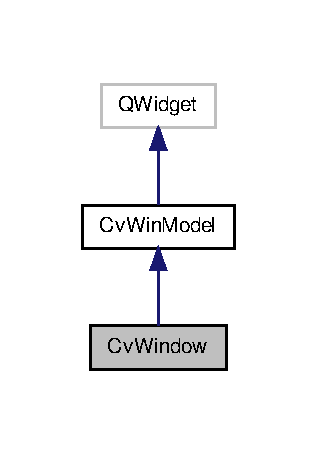
\includegraphics[width=152pt]{classCvWindow__inherit__graph}
\end{center}
\end{figure}


Collaboration diagram for Cv\-Window\-:
\nopagebreak
\begin{figure}[H]
\begin{center}
\leavevmode
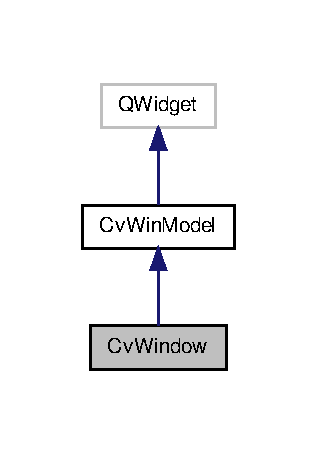
\includegraphics[width=152pt]{classCvWindow__coll__graph}
\end{center}
\end{figure}
\subsection*{Public Member Functions}
\begin{DoxyCompactItemize}
\item 
\hyperlink{classCvWindow_a2d516104e7e29c293d53a3797f29fff6}{Cv\-Window} (Q\-String arg2, int flag=C\-V\-\_\-\-W\-I\-N\-D\-O\-W\-\_\-\-N\-O\-R\-M\-A\-L)
\item 
\hyperlink{classCvWindow_aac9ea5f91071477dc506ed9a04f758f1}{$\sim$\-Cv\-Window} ()
\item 
void \hyperlink{classCvWindow_a8fa9463b57ffb2f049703a6f14e586fb}{set\-Mouse\-Call\-Back} (Cv\-Mouse\-Callback m, void $\ast$param)
\item 
void \hyperlink{classCvWindow_a9fc4a9246e0ea710076d2d58851ce1f8}{update\-Image} (void $\ast$arr)
\item 
void \hyperlink{classCvWindow_a577841174681451e47735cc125de0af9}{display\-Info} (Q\-String text, int delayms)
\item 
void \hyperlink{classCvWindow_a37a9d43cf4e722abbb32a20fc507c8a9}{display\-Status\-Bar} (Q\-String text, int delayms)
\item 
void \hyperlink{classCvWindow_a7f8fdaeec81ca1900a8878bdfc779f13}{read\-Settings} ()
\item 
void \hyperlink{classCvWindow_a30c9687c99f22a7f7d9a61c00bf42a57}{write\-Settings} ()
\item 
void \hyperlink{classCvWindow_a40da445af152145b663ebdc5a2547351}{hide\-Tools} ()
\item 
void \hyperlink{classCvWindow_a0e911ed5861b7d39a991671af7aabfbc}{show\-Tools} ()
\item 
Q\-Size \hyperlink{classCvWindow_a323bcaa31cfe862e2b13a110248293cc}{get\-Available\-Size} ()
\item 
\hyperlink{classViewPort}{View\-Port} $\ast$ \hyperlink{classCvWindow_a6bfa17ceb41e3fad856b9dd32d25e048}{get\-View} ()
\end{DoxyCompactItemize}
\subsection*{Static Public Member Functions}
\begin{DoxyCompactItemize}
\item 
static void \hyperlink{classCvWindow_a2ed13c03bc5fa9fd2e7b579d2fc1bd6d}{add\-Slider} (\hyperlink{classCvWindow}{Cv\-Window} $\ast$w, Q\-String name, int $\ast$value, int count, Cv\-Trackbar\-Callback on\-\_\-change C\-V\-\_\-\-D\-E\-F\-A\-U\-L\-T(N\-U\-L\-L))
\item 
static void \hyperlink{classCvWindow_a87c0aa2a8a5986293be621a9f949e33e}{add\-Slider2} (\hyperlink{classCvWindow}{Cv\-Window} $\ast$w, Q\-String name, int $\ast$value, int count, Cv\-Trackbar\-Callback2 on\-\_\-change C\-V\-\_\-\-D\-E\-F\-A\-U\-L\-T(N\-U\-L\-L), void $\ast$userdata C\-V\-\_\-\-D\-E\-F\-A\-U\-L\-T(0))
\item 
static \hyperlink{classCvButtonbar}{Cv\-Buttonbar} $\ast$ \hyperlink{classCvWindow_a219c9032d1611f4e394eae3dea4011ab}{create\-Buttonbar} (Q\-String bar\-\_\-name)
\end{DoxyCompactItemize}
\subsection*{Data Fields}
\begin{DoxyCompactItemize}
\item 
Q\-Pointer$<$ Q\-Box\-Layout $>$ \hyperlink{classCvWindow_a706d24419e22947d0fcdcef9d3194605}{my\-Global\-Layout}
\item 
Q\-Pointer$<$ Q\-Box\-Layout $>$ \hyperlink{classCvWindow_a1c1ba7aa00c19ca8a99da650f8bd6fb1}{my\-Bar\-Layout}
\item 
Q\-Pointer$<$ Q\-Status\-Bar $>$ \hyperlink{classCvWindow_ad21a9548c597a6651b73d41a3383a1d3}{my\-Status\-Bar}
\item 
Q\-Pointer$<$ Q\-Tool\-Bar $>$ \hyperlink{classCvWindow_a147b82422fa5d532192990f77e6ae2d8}{my\-Tool\-Bar}
\item 
Q\-Pointer$<$ Q\-Label $>$ \hyperlink{classCvWindow_a62c523f9df3830591bcbb44145c85db4}{my\-Status\-Bar\-\_\-msg}
\item 
Q\-String \hyperlink{classCvWindow_a2f2e2a14703dbe479049862f5f43ac13}{param\-\_\-name}
\item 
int \hyperlink{classCvWindow_ae79962eeb12c2dbcedafb23362ba1847}{param\-\_\-flags}
\item 
int \hyperlink{classCvWindow_a1503f81d43bec919c329a1c98cb3f559}{param\-\_\-gui\-\_\-mode}
\item 
int \hyperlink{classCvWindow_a9d97fe990d3fb23daa031ac39483b059}{param\-\_\-ratio\-\_\-mode}
\item 
Q\-Vector$<$ Q\-Action $\ast$ $>$ \hyperlink{classCvWindow_a55d09660aba2ef83bf2eaa4fe80bb746}{vect\-\_\-\-Q\-Actions}
\end{DoxyCompactItemize}


\subsection{Constructor \& Destructor Documentation}
\hypertarget{classCvWindow_a2d516104e7e29c293d53a3797f29fff6}{\index{Cv\-Window@{Cv\-Window}!Cv\-Window@{Cv\-Window}}
\index{Cv\-Window@{Cv\-Window}!CvWindow@{Cv\-Window}}
\subsubsection[{Cv\-Window}]{\setlength{\rightskip}{0pt plus 5cm}Cv\-Window\-::\-Cv\-Window (
\begin{DoxyParamCaption}
\item[{Q\-String}]{arg2, }
\item[{int}]{flag = {\ttfamily CV\-\_\-WINDOW\-\_\-NORMAL}}
\end{DoxyParamCaption}
)}}\label{classCvWindow_a2d516104e7e29c293d53a3797f29fff6}
\hypertarget{classCvWindow_aac9ea5f91071477dc506ed9a04f758f1}{\index{Cv\-Window@{Cv\-Window}!$\sim$\-Cv\-Window@{$\sim$\-Cv\-Window}}
\index{$\sim$\-Cv\-Window@{$\sim$\-Cv\-Window}!CvWindow@{Cv\-Window}}
\subsubsection[{$\sim$\-Cv\-Window}]{\setlength{\rightskip}{0pt plus 5cm}Cv\-Window\-::$\sim$\-Cv\-Window (
\begin{DoxyParamCaption}
{}
\end{DoxyParamCaption}
)}}\label{classCvWindow_aac9ea5f91071477dc506ed9a04f758f1}


\subsection{Member Function Documentation}
\hypertarget{classCvWindow_a2ed13c03bc5fa9fd2e7b579d2fc1bd6d}{\index{Cv\-Window@{Cv\-Window}!add\-Slider@{add\-Slider}}
\index{add\-Slider@{add\-Slider}!CvWindow@{Cv\-Window}}
\subsubsection[{add\-Slider}]{\setlength{\rightskip}{0pt plus 5cm}void Cv\-Window\-::add\-Slider (
\begin{DoxyParamCaption}
\item[{{\bf Cv\-Window} $\ast$}]{w, }
\item[{Q\-String}]{name, }
\item[{int $\ast$}]{value, }
\item[{int}]{count, }
\item[{Cv\-Trackbar\-Callback on\-\_\-change }]{C\-V\-\_\-\-D\-E\-F\-A\-U\-L\-TN\-U\-L\-L}
\end{DoxyParamCaption}
)\hspace{0.3cm}{\ttfamily [static]}}}\label{classCvWindow_a2ed13c03bc5fa9fd2e7b579d2fc1bd6d}
\hypertarget{classCvWindow_a87c0aa2a8a5986293be621a9f949e33e}{\index{Cv\-Window@{Cv\-Window}!add\-Slider2@{add\-Slider2}}
\index{add\-Slider2@{add\-Slider2}!CvWindow@{Cv\-Window}}
\subsubsection[{add\-Slider2}]{\setlength{\rightskip}{0pt plus 5cm}void Cv\-Window\-::add\-Slider2 (
\begin{DoxyParamCaption}
\item[{{\bf Cv\-Window} $\ast$}]{w, }
\item[{Q\-String}]{name, }
\item[{int $\ast$}]{value, }
\item[{int}]{count, }
\item[{Cv\-Trackbar\-Callback2 on\-\_\-change }]{C\-V\-\_\-\-D\-E\-F\-A\-U\-L\-TN\-U\-L\-L, }
\item[{void $\ast$userdata }]{C\-V\-\_\-\-D\-E\-F\-A\-U\-L\-T0}
\end{DoxyParamCaption}
)\hspace{0.3cm}{\ttfamily [static]}}}\label{classCvWindow_a87c0aa2a8a5986293be621a9f949e33e}
\hypertarget{classCvWindow_a219c9032d1611f4e394eae3dea4011ab}{\index{Cv\-Window@{Cv\-Window}!create\-Buttonbar@{create\-Buttonbar}}
\index{create\-Buttonbar@{create\-Buttonbar}!CvWindow@{Cv\-Window}}
\subsubsection[{create\-Buttonbar}]{\setlength{\rightskip}{0pt plus 5cm}{\bf Cv\-Buttonbar} $\ast$ Cv\-Window\-::create\-Buttonbar (
\begin{DoxyParamCaption}
\item[{Q\-String}]{bar\-\_\-name}
\end{DoxyParamCaption}
)\hspace{0.3cm}{\ttfamily [static]}}}\label{classCvWindow_a219c9032d1611f4e394eae3dea4011ab}
\hypertarget{classCvWindow_a577841174681451e47735cc125de0af9}{\index{Cv\-Window@{Cv\-Window}!display\-Info@{display\-Info}}
\index{display\-Info@{display\-Info}!CvWindow@{Cv\-Window}}
\subsubsection[{display\-Info}]{\setlength{\rightskip}{0pt plus 5cm}void Cv\-Window\-::display\-Info (
\begin{DoxyParamCaption}
\item[{Q\-String}]{text, }
\item[{int}]{delayms}
\end{DoxyParamCaption}
)}}\label{classCvWindow_a577841174681451e47735cc125de0af9}
\hypertarget{classCvWindow_a37a9d43cf4e722abbb32a20fc507c8a9}{\index{Cv\-Window@{Cv\-Window}!display\-Status\-Bar@{display\-Status\-Bar}}
\index{display\-Status\-Bar@{display\-Status\-Bar}!CvWindow@{Cv\-Window}}
\subsubsection[{display\-Status\-Bar}]{\setlength{\rightskip}{0pt plus 5cm}void Cv\-Window\-::display\-Status\-Bar (
\begin{DoxyParamCaption}
\item[{Q\-String}]{text, }
\item[{int}]{delayms}
\end{DoxyParamCaption}
)}}\label{classCvWindow_a37a9d43cf4e722abbb32a20fc507c8a9}
\hypertarget{classCvWindow_a323bcaa31cfe862e2b13a110248293cc}{\index{Cv\-Window@{Cv\-Window}!get\-Available\-Size@{get\-Available\-Size}}
\index{get\-Available\-Size@{get\-Available\-Size}!CvWindow@{Cv\-Window}}
\subsubsection[{get\-Available\-Size}]{\setlength{\rightskip}{0pt plus 5cm}Q\-Size Cv\-Window\-::get\-Available\-Size (
\begin{DoxyParamCaption}
{}
\end{DoxyParamCaption}
)}}\label{classCvWindow_a323bcaa31cfe862e2b13a110248293cc}
\hypertarget{classCvWindow_a6bfa17ceb41e3fad856b9dd32d25e048}{\index{Cv\-Window@{Cv\-Window}!get\-View@{get\-View}}
\index{get\-View@{get\-View}!CvWindow@{Cv\-Window}}
\subsubsection[{get\-View}]{\setlength{\rightskip}{0pt plus 5cm}{\bf View\-Port} $\ast$ Cv\-Window\-::get\-View (
\begin{DoxyParamCaption}
{}
\end{DoxyParamCaption}
)}}\label{classCvWindow_a6bfa17ceb41e3fad856b9dd32d25e048}
\hypertarget{classCvWindow_a40da445af152145b663ebdc5a2547351}{\index{Cv\-Window@{Cv\-Window}!hide\-Tools@{hide\-Tools}}
\index{hide\-Tools@{hide\-Tools}!CvWindow@{Cv\-Window}}
\subsubsection[{hide\-Tools}]{\setlength{\rightskip}{0pt plus 5cm}void Cv\-Window\-::hide\-Tools (
\begin{DoxyParamCaption}
{}
\end{DoxyParamCaption}
)}}\label{classCvWindow_a40da445af152145b663ebdc5a2547351}
\hypertarget{classCvWindow_a7f8fdaeec81ca1900a8878bdfc779f13}{\index{Cv\-Window@{Cv\-Window}!read\-Settings@{read\-Settings}}
\index{read\-Settings@{read\-Settings}!CvWindow@{Cv\-Window}}
\subsubsection[{read\-Settings}]{\setlength{\rightskip}{0pt plus 5cm}void Cv\-Window\-::read\-Settings (
\begin{DoxyParamCaption}
{}
\end{DoxyParamCaption}
)}}\label{classCvWindow_a7f8fdaeec81ca1900a8878bdfc779f13}
\hypertarget{classCvWindow_a8fa9463b57ffb2f049703a6f14e586fb}{\index{Cv\-Window@{Cv\-Window}!set\-Mouse\-Call\-Back@{set\-Mouse\-Call\-Back}}
\index{set\-Mouse\-Call\-Back@{set\-Mouse\-Call\-Back}!CvWindow@{Cv\-Window}}
\subsubsection[{set\-Mouse\-Call\-Back}]{\setlength{\rightskip}{0pt plus 5cm}void Cv\-Window\-::set\-Mouse\-Call\-Back (
\begin{DoxyParamCaption}
\item[{Cv\-Mouse\-Callback}]{m, }
\item[{void $\ast$}]{param}
\end{DoxyParamCaption}
)}}\label{classCvWindow_a8fa9463b57ffb2f049703a6f14e586fb}
\hypertarget{classCvWindow_a0e911ed5861b7d39a991671af7aabfbc}{\index{Cv\-Window@{Cv\-Window}!show\-Tools@{show\-Tools}}
\index{show\-Tools@{show\-Tools}!CvWindow@{Cv\-Window}}
\subsubsection[{show\-Tools}]{\setlength{\rightskip}{0pt plus 5cm}void Cv\-Window\-::show\-Tools (
\begin{DoxyParamCaption}
{}
\end{DoxyParamCaption}
)}}\label{classCvWindow_a0e911ed5861b7d39a991671af7aabfbc}
\hypertarget{classCvWindow_a9fc4a9246e0ea710076d2d58851ce1f8}{\index{Cv\-Window@{Cv\-Window}!update\-Image@{update\-Image}}
\index{update\-Image@{update\-Image}!CvWindow@{Cv\-Window}}
\subsubsection[{update\-Image}]{\setlength{\rightskip}{0pt plus 5cm}void Cv\-Window\-::update\-Image (
\begin{DoxyParamCaption}
\item[{void $\ast$}]{arr}
\end{DoxyParamCaption}
)}}\label{classCvWindow_a9fc4a9246e0ea710076d2d58851ce1f8}
\hypertarget{classCvWindow_a30c9687c99f22a7f7d9a61c00bf42a57}{\index{Cv\-Window@{Cv\-Window}!write\-Settings@{write\-Settings}}
\index{write\-Settings@{write\-Settings}!CvWindow@{Cv\-Window}}
\subsubsection[{write\-Settings}]{\setlength{\rightskip}{0pt plus 5cm}void Cv\-Window\-::write\-Settings (
\begin{DoxyParamCaption}
{}
\end{DoxyParamCaption}
)}}\label{classCvWindow_a30c9687c99f22a7f7d9a61c00bf42a57}


\subsection{Field Documentation}
\hypertarget{classCvWindow_a1c1ba7aa00c19ca8a99da650f8bd6fb1}{\index{Cv\-Window@{Cv\-Window}!my\-Bar\-Layout@{my\-Bar\-Layout}}
\index{my\-Bar\-Layout@{my\-Bar\-Layout}!CvWindow@{Cv\-Window}}
\subsubsection[{my\-Bar\-Layout}]{\setlength{\rightskip}{0pt plus 5cm}Q\-Pointer$<$Q\-Box\-Layout$>$ Cv\-Window\-::my\-Bar\-Layout}}\label{classCvWindow_a1c1ba7aa00c19ca8a99da650f8bd6fb1}
\hypertarget{classCvWindow_a706d24419e22947d0fcdcef9d3194605}{\index{Cv\-Window@{Cv\-Window}!my\-Global\-Layout@{my\-Global\-Layout}}
\index{my\-Global\-Layout@{my\-Global\-Layout}!CvWindow@{Cv\-Window}}
\subsubsection[{my\-Global\-Layout}]{\setlength{\rightskip}{0pt plus 5cm}Q\-Pointer$<$Q\-Box\-Layout$>$ Cv\-Window\-::my\-Global\-Layout}}\label{classCvWindow_a706d24419e22947d0fcdcef9d3194605}
\hypertarget{classCvWindow_ad21a9548c597a6651b73d41a3383a1d3}{\index{Cv\-Window@{Cv\-Window}!my\-Status\-Bar@{my\-Status\-Bar}}
\index{my\-Status\-Bar@{my\-Status\-Bar}!CvWindow@{Cv\-Window}}
\subsubsection[{my\-Status\-Bar}]{\setlength{\rightskip}{0pt plus 5cm}Q\-Pointer$<$Q\-Status\-Bar$>$ Cv\-Window\-::my\-Status\-Bar}}\label{classCvWindow_ad21a9548c597a6651b73d41a3383a1d3}
\hypertarget{classCvWindow_a62c523f9df3830591bcbb44145c85db4}{\index{Cv\-Window@{Cv\-Window}!my\-Status\-Bar\-\_\-msg@{my\-Status\-Bar\-\_\-msg}}
\index{my\-Status\-Bar\-\_\-msg@{my\-Status\-Bar\-\_\-msg}!CvWindow@{Cv\-Window}}
\subsubsection[{my\-Status\-Bar\-\_\-msg}]{\setlength{\rightskip}{0pt plus 5cm}Q\-Pointer$<$Q\-Label$>$ Cv\-Window\-::my\-Status\-Bar\-\_\-msg}}\label{classCvWindow_a62c523f9df3830591bcbb44145c85db4}
\hypertarget{classCvWindow_a147b82422fa5d532192990f77e6ae2d8}{\index{Cv\-Window@{Cv\-Window}!my\-Tool\-Bar@{my\-Tool\-Bar}}
\index{my\-Tool\-Bar@{my\-Tool\-Bar}!CvWindow@{Cv\-Window}}
\subsubsection[{my\-Tool\-Bar}]{\setlength{\rightskip}{0pt plus 5cm}Q\-Pointer$<$Q\-Tool\-Bar$>$ Cv\-Window\-::my\-Tool\-Bar}}\label{classCvWindow_a147b82422fa5d532192990f77e6ae2d8}
\hypertarget{classCvWindow_ae79962eeb12c2dbcedafb23362ba1847}{\index{Cv\-Window@{Cv\-Window}!param\-\_\-flags@{param\-\_\-flags}}
\index{param\-\_\-flags@{param\-\_\-flags}!CvWindow@{Cv\-Window}}
\subsubsection[{param\-\_\-flags}]{\setlength{\rightskip}{0pt plus 5cm}int Cv\-Window\-::param\-\_\-flags}}\label{classCvWindow_ae79962eeb12c2dbcedafb23362ba1847}
\hypertarget{classCvWindow_a1503f81d43bec919c329a1c98cb3f559}{\index{Cv\-Window@{Cv\-Window}!param\-\_\-gui\-\_\-mode@{param\-\_\-gui\-\_\-mode}}
\index{param\-\_\-gui\-\_\-mode@{param\-\_\-gui\-\_\-mode}!CvWindow@{Cv\-Window}}
\subsubsection[{param\-\_\-gui\-\_\-mode}]{\setlength{\rightskip}{0pt plus 5cm}int Cv\-Window\-::param\-\_\-gui\-\_\-mode}}\label{classCvWindow_a1503f81d43bec919c329a1c98cb3f559}
\hypertarget{classCvWindow_a2f2e2a14703dbe479049862f5f43ac13}{\index{Cv\-Window@{Cv\-Window}!param\-\_\-name@{param\-\_\-name}}
\index{param\-\_\-name@{param\-\_\-name}!CvWindow@{Cv\-Window}}
\subsubsection[{param\-\_\-name}]{\setlength{\rightskip}{0pt plus 5cm}Q\-String Cv\-Window\-::param\-\_\-name}}\label{classCvWindow_a2f2e2a14703dbe479049862f5f43ac13}
\hypertarget{classCvWindow_a9d97fe990d3fb23daa031ac39483b059}{\index{Cv\-Window@{Cv\-Window}!param\-\_\-ratio\-\_\-mode@{param\-\_\-ratio\-\_\-mode}}
\index{param\-\_\-ratio\-\_\-mode@{param\-\_\-ratio\-\_\-mode}!CvWindow@{Cv\-Window}}
\subsubsection[{param\-\_\-ratio\-\_\-mode}]{\setlength{\rightskip}{0pt plus 5cm}int Cv\-Window\-::param\-\_\-ratio\-\_\-mode}}\label{classCvWindow_a9d97fe990d3fb23daa031ac39483b059}
\hypertarget{classCvWindow_a55d09660aba2ef83bf2eaa4fe80bb746}{\index{Cv\-Window@{Cv\-Window}!vect\-\_\-\-Q\-Actions@{vect\-\_\-\-Q\-Actions}}
\index{vect\-\_\-\-Q\-Actions@{vect\-\_\-\-Q\-Actions}!CvWindow@{Cv\-Window}}
\subsubsection[{vect\-\_\-\-Q\-Actions}]{\setlength{\rightskip}{0pt plus 5cm}Q\-Vector$<$Q\-Action$\ast$$>$ Cv\-Window\-::vect\-\_\-\-Q\-Actions}}\label{classCvWindow_a55d09660aba2ef83bf2eaa4fe80bb746}


The documentation for this class was generated from the following files\-:\begin{DoxyCompactItemize}
\item 
\hyperlink{window__QT_8h}{window\-\_\-\-Q\-T.\-h}\item 
\hyperlink{window__QT_8cpp}{window\-\_\-\-Q\-T.\-cpp}\end{DoxyCompactItemize}

\hypertarget{classCvWinModel}{
\section{CvWinModel Class Reference}
\label{classCvWinModel}\index{CvWinModel@{CvWinModel}}
}


{\ttfamily \#include $<$window\_\-QT.h$>$}



Inheritance diagram for CvWinModel:\nopagebreak
\begin{figure}[H]
\begin{center}
\leavevmode
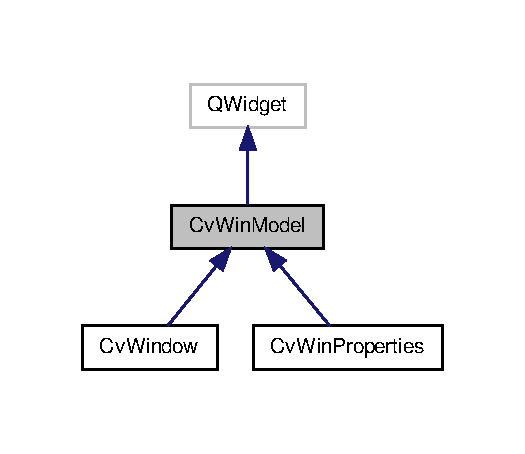
\includegraphics[width=210pt]{classCvWinModel__inherit__graph}
\end{center}
\end{figure}
\subsection*{Data Fields}
\begin{DoxyCompactItemize}
\item 
\hyperlink{window__QT_8h_a3ce3f41fe742c83e94d4cd007e7b4c70}{typeWindow} \hyperlink{classCvWinModel_a6b9598fed3bff14f0c10ec85a20ed83e}{type}
\end{DoxyCompactItemize}


\subsection{Field Documentation}
\hypertarget{classCvWinModel_a6b9598fed3bff14f0c10ec85a20ed83e}{
\index{CvWinModel@{CvWinModel}!type@{type}}
\index{type@{type}!CvWinModel@{CvWinModel}}
\subsubsection[{type}]{\setlength{\rightskip}{0pt plus 5cm}{\bf typeWindow} {\bf CvWinModel::type}}}
\label{classCvWinModel_a6b9598fed3bff14f0c10ec85a20ed83e}


The documentation for this class was generated from the following file:\begin{DoxyCompactItemize}
\item 
\hyperlink{window__QT_8h}{window\_\-QT.h}\end{DoxyCompactItemize}

\hypertarget{classCvWinProperties}{\section{Cv\-Win\-Properties Class Reference}
\label{classCvWinProperties}\index{Cv\-Win\-Properties@{Cv\-Win\-Properties}}
}


{\ttfamily \#include $<$window\-\_\-\-Q\-T.\-h$>$}



Inheritance diagram for Cv\-Win\-Properties\-:
\nopagebreak
\begin{figure}[H]
\begin{center}
\leavevmode
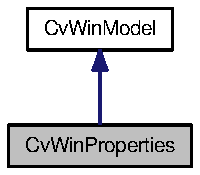
\includegraphics[width=170pt]{classCvWinProperties__inherit__graph}
\end{center}
\end{figure}


Collaboration diagram for Cv\-Win\-Properties\-:
\nopagebreak
\begin{figure}[H]
\begin{center}
\leavevmode
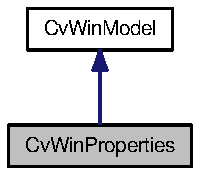
\includegraphics[width=170pt]{classCvWinProperties__coll__graph}
\end{center}
\end{figure}
\subsection*{Public Member Functions}
\begin{DoxyCompactItemize}
\item 
\hyperlink{classCvWinProperties_a916ba2a24b09baaa9bb9efd7d16606e3}{Cv\-Win\-Properties} (Q\-String name, Q\-Object $\ast$parent)
\item 
\hyperlink{classCvWinProperties_a0953344aa7f41767c0da7ee59b17e0bb}{$\sim$\-Cv\-Win\-Properties} ()
\end{DoxyCompactItemize}
\subsection*{Data Fields}
\begin{DoxyCompactItemize}
\item 
Q\-Pointer$<$ Q\-Box\-Layout $>$ \hyperlink{classCvWinProperties_a7b02e9dde3e939c4a3f7126f116247af}{my\-Layout}
\end{DoxyCompactItemize}


\subsection{Constructor \& Destructor Documentation}
\hypertarget{classCvWinProperties_a916ba2a24b09baaa9bb9efd7d16606e3}{\index{Cv\-Win\-Properties@{Cv\-Win\-Properties}!Cv\-Win\-Properties@{Cv\-Win\-Properties}}
\index{Cv\-Win\-Properties@{Cv\-Win\-Properties}!CvWinProperties@{Cv\-Win\-Properties}}
\subsubsection[{Cv\-Win\-Properties}]{\setlength{\rightskip}{0pt plus 5cm}Cv\-Win\-Properties\-::\-Cv\-Win\-Properties (
\begin{DoxyParamCaption}
\item[{Q\-String}]{name, }
\item[{Q\-Object $\ast$}]{parent}
\end{DoxyParamCaption}
)}}\label{classCvWinProperties_a916ba2a24b09baaa9bb9efd7d16606e3}
\hypertarget{classCvWinProperties_a0953344aa7f41767c0da7ee59b17e0bb}{\index{Cv\-Win\-Properties@{Cv\-Win\-Properties}!$\sim$\-Cv\-Win\-Properties@{$\sim$\-Cv\-Win\-Properties}}
\index{$\sim$\-Cv\-Win\-Properties@{$\sim$\-Cv\-Win\-Properties}!CvWinProperties@{Cv\-Win\-Properties}}
\subsubsection[{$\sim$\-Cv\-Win\-Properties}]{\setlength{\rightskip}{0pt plus 5cm}Cv\-Win\-Properties\-::$\sim$\-Cv\-Win\-Properties (
\begin{DoxyParamCaption}
{}
\end{DoxyParamCaption}
)}}\label{classCvWinProperties_a0953344aa7f41767c0da7ee59b17e0bb}


\subsection{Field Documentation}
\hypertarget{classCvWinProperties_a7b02e9dde3e939c4a3f7126f116247af}{\index{Cv\-Win\-Properties@{Cv\-Win\-Properties}!my\-Layout@{my\-Layout}}
\index{my\-Layout@{my\-Layout}!CvWinProperties@{Cv\-Win\-Properties}}
\subsubsection[{my\-Layout}]{\setlength{\rightskip}{0pt plus 5cm}Q\-Pointer$<$Q\-Box\-Layout$>$ Cv\-Win\-Properties\-::my\-Layout}}\label{classCvWinProperties_a7b02e9dde3e939c4a3f7126f116247af}


The documentation for this class was generated from the following files\-:\begin{DoxyCompactItemize}
\item 
\hyperlink{window__QT_8h}{window\-\_\-\-Q\-T.\-h}\item 
\hyperlink{window__QT_8cpp}{window\-\_\-\-Q\-T.\-cpp}\end{DoxyCompactItemize}

\hypertarget{classDepthFaceDetector}{\section{Depth\-Face\-Detector Class Reference}
\label{classDepthFaceDetector}\index{Depth\-Face\-Detector@{Depth\-Face\-Detector}}
}


{\ttfamily \#include $<$Depth\-Face\-Detector.\-h$>$}

\subsection*{Public Member Functions}
\begin{DoxyCompactItemize}
\item 
\hyperlink{classDepthFaceDetector_a1efe4e883faaad6a33acd0909e1ec282}{Depth\-Face\-Detector} (void)
\item 
vector$<$ Rect $>$ \hyperlink{classDepthFaceDetector_ace3a3506a58be0d500d866d1574a35be}{detect\-\_\-face\-\_\-depth} (Mat \hyperlink{social__robot__onethread_8cpp_a5b613972ff73fd7b34e0ee18acc5c1a6}{depth\-\_\-image}, Mat \hyperlink{social__robot__onethread_8cpp_a485c05800d39168b94f859fac62aa6a7}{disparity\-\_\-image})
\end{DoxyCompactItemize}
\subsection*{Data Fields}
\begin{DoxyCompactItemize}
\item 
double \hyperlink{classDepthFaceDetector_a284b331a23267ac39e84059541df3351}{canny\-\_\-thr1}
\item 
double \hyperlink{classDepthFaceDetector_acb512932956d9d2e366ed0dbea349a77}{canny\-\_\-thr2}
\item 
double \hyperlink{classDepthFaceDetector_a000af3e2a38d75b54e4e7f9a2f372844}{chamfer\-\_\-thr}
\item 
double \hyperlink{classDepthFaceDetector_a95b723b80aaf14713aae8a5d763d3202}{arc\-\_\-thr\-\_\-low}
\item 
double \hyperlink{classDepthFaceDetector_a494d138048f11fa59da7cdd864c3b7fa}{arc\-\_\-thr\-\_\-high}
\item 
double \hyperlink{classDepthFaceDetector_ae3413e4a8064c92a69300c5adbd8e3ed}{approx\-\_\-poly\-\_\-thr}
\item 
double \hyperlink{classDepthFaceDetector_a6d26a22f8f85dc4e70ba368b52241882}{max\-\_\-suppression}
\item 
double \hyperlink{classDepthFaceDetector_a4dbe7bcae76b86b9dce3383e8da0fb87}{scale\-\_\-factor}
\item 
double \hyperlink{classDepthFaceDetector_ad2d08e90624566d7bd6e51e141edb1a6}{match3\-D\-\_\-thr}
\item 
int \hyperlink{classDepthFaceDetector_ab2a61535fe93d7df87e6a37c584f9819}{scales}
\item 
int \hyperlink{classDepthFaceDetector_a1bf21c5a6c326bba9f5710c207d1555f}{scales\-\_\-default}
\item 
int \hyperlink{classDepthFaceDetector_a48a0fc86ac4fcbf0347a0247557b5f29}{framenum}
\item 
int \hyperlink{classDepthFaceDetector_ace0000695ed60a214c65e82793f53c7c}{update\-\_\-rate}
\end{DoxyCompactItemize}


\subsection{Constructor \& Destructor Documentation}
\hypertarget{classDepthFaceDetector_a1efe4e883faaad6a33acd0909e1ec282}{\index{Depth\-Face\-Detector@{Depth\-Face\-Detector}!Depth\-Face\-Detector@{Depth\-Face\-Detector}}
\index{Depth\-Face\-Detector@{Depth\-Face\-Detector}!DepthFaceDetector@{Depth\-Face\-Detector}}
\subsubsection[{Depth\-Face\-Detector}]{\setlength{\rightskip}{0pt plus 5cm}Depth\-Face\-Detector\-::\-Depth\-Face\-Detector (
\begin{DoxyParamCaption}
\item[{void}]{}
\end{DoxyParamCaption}
)}}\label{classDepthFaceDetector_a1efe4e883faaad6a33acd0909e1ec282}


\subsection{Member Function Documentation}
\hypertarget{classDepthFaceDetector_ace3a3506a58be0d500d866d1574a35be}{\index{Depth\-Face\-Detector@{Depth\-Face\-Detector}!detect\-\_\-face\-\_\-depth@{detect\-\_\-face\-\_\-depth}}
\index{detect\-\_\-face\-\_\-depth@{detect\-\_\-face\-\_\-depth}!DepthFaceDetector@{Depth\-Face\-Detector}}
\subsubsection[{detect\-\_\-face\-\_\-depth}]{\setlength{\rightskip}{0pt plus 5cm}vector$<$ Rect $>$ Depth\-Face\-Detector\-::detect\-\_\-face\-\_\-depth (
\begin{DoxyParamCaption}
\item[{Mat}]{depth\-\_\-image, }
\item[{Mat}]{disparity\-\_\-image}
\end{DoxyParamCaption}
)}}\label{classDepthFaceDetector_ace3a3506a58be0d500d866d1574a35be}


\subsection{Field Documentation}
\hypertarget{classDepthFaceDetector_ae3413e4a8064c92a69300c5adbd8e3ed}{\index{Depth\-Face\-Detector@{Depth\-Face\-Detector}!approx\-\_\-poly\-\_\-thr@{approx\-\_\-poly\-\_\-thr}}
\index{approx\-\_\-poly\-\_\-thr@{approx\-\_\-poly\-\_\-thr}!DepthFaceDetector@{Depth\-Face\-Detector}}
\subsubsection[{approx\-\_\-poly\-\_\-thr}]{\setlength{\rightskip}{0pt plus 5cm}double Depth\-Face\-Detector\-::approx\-\_\-poly\-\_\-thr}}\label{classDepthFaceDetector_ae3413e4a8064c92a69300c5adbd8e3ed}
\hypertarget{classDepthFaceDetector_a494d138048f11fa59da7cdd864c3b7fa}{\index{Depth\-Face\-Detector@{Depth\-Face\-Detector}!arc\-\_\-thr\-\_\-high@{arc\-\_\-thr\-\_\-high}}
\index{arc\-\_\-thr\-\_\-high@{arc\-\_\-thr\-\_\-high}!DepthFaceDetector@{Depth\-Face\-Detector}}
\subsubsection[{arc\-\_\-thr\-\_\-high}]{\setlength{\rightskip}{0pt plus 5cm}double Depth\-Face\-Detector\-::arc\-\_\-thr\-\_\-high}}\label{classDepthFaceDetector_a494d138048f11fa59da7cdd864c3b7fa}
\hypertarget{classDepthFaceDetector_a95b723b80aaf14713aae8a5d763d3202}{\index{Depth\-Face\-Detector@{Depth\-Face\-Detector}!arc\-\_\-thr\-\_\-low@{arc\-\_\-thr\-\_\-low}}
\index{arc\-\_\-thr\-\_\-low@{arc\-\_\-thr\-\_\-low}!DepthFaceDetector@{Depth\-Face\-Detector}}
\subsubsection[{arc\-\_\-thr\-\_\-low}]{\setlength{\rightskip}{0pt plus 5cm}double Depth\-Face\-Detector\-::arc\-\_\-thr\-\_\-low}}\label{classDepthFaceDetector_a95b723b80aaf14713aae8a5d763d3202}
\hypertarget{classDepthFaceDetector_a284b331a23267ac39e84059541df3351}{\index{Depth\-Face\-Detector@{Depth\-Face\-Detector}!canny\-\_\-thr1@{canny\-\_\-thr1}}
\index{canny\-\_\-thr1@{canny\-\_\-thr1}!DepthFaceDetector@{Depth\-Face\-Detector}}
\subsubsection[{canny\-\_\-thr1}]{\setlength{\rightskip}{0pt plus 5cm}double Depth\-Face\-Detector\-::canny\-\_\-thr1}}\label{classDepthFaceDetector_a284b331a23267ac39e84059541df3351}
\hypertarget{classDepthFaceDetector_acb512932956d9d2e366ed0dbea349a77}{\index{Depth\-Face\-Detector@{Depth\-Face\-Detector}!canny\-\_\-thr2@{canny\-\_\-thr2}}
\index{canny\-\_\-thr2@{canny\-\_\-thr2}!DepthFaceDetector@{Depth\-Face\-Detector}}
\subsubsection[{canny\-\_\-thr2}]{\setlength{\rightskip}{0pt plus 5cm}double Depth\-Face\-Detector\-::canny\-\_\-thr2}}\label{classDepthFaceDetector_acb512932956d9d2e366ed0dbea349a77}
\hypertarget{classDepthFaceDetector_a000af3e2a38d75b54e4e7f9a2f372844}{\index{Depth\-Face\-Detector@{Depth\-Face\-Detector}!chamfer\-\_\-thr@{chamfer\-\_\-thr}}
\index{chamfer\-\_\-thr@{chamfer\-\_\-thr}!DepthFaceDetector@{Depth\-Face\-Detector}}
\subsubsection[{chamfer\-\_\-thr}]{\setlength{\rightskip}{0pt plus 5cm}double Depth\-Face\-Detector\-::chamfer\-\_\-thr}}\label{classDepthFaceDetector_a000af3e2a38d75b54e4e7f9a2f372844}
\hypertarget{classDepthFaceDetector_a48a0fc86ac4fcbf0347a0247557b5f29}{\index{Depth\-Face\-Detector@{Depth\-Face\-Detector}!framenum@{framenum}}
\index{framenum@{framenum}!DepthFaceDetector@{Depth\-Face\-Detector}}
\subsubsection[{framenum}]{\setlength{\rightskip}{0pt plus 5cm}int Depth\-Face\-Detector\-::framenum}}\label{classDepthFaceDetector_a48a0fc86ac4fcbf0347a0247557b5f29}
\hypertarget{classDepthFaceDetector_ad2d08e90624566d7bd6e51e141edb1a6}{\index{Depth\-Face\-Detector@{Depth\-Face\-Detector}!match3\-D\-\_\-thr@{match3\-D\-\_\-thr}}
\index{match3\-D\-\_\-thr@{match3\-D\-\_\-thr}!DepthFaceDetector@{Depth\-Face\-Detector}}
\subsubsection[{match3\-D\-\_\-thr}]{\setlength{\rightskip}{0pt plus 5cm}double Depth\-Face\-Detector\-::match3\-D\-\_\-thr}}\label{classDepthFaceDetector_ad2d08e90624566d7bd6e51e141edb1a6}
\hypertarget{classDepthFaceDetector_a6d26a22f8f85dc4e70ba368b52241882}{\index{Depth\-Face\-Detector@{Depth\-Face\-Detector}!max\-\_\-suppression@{max\-\_\-suppression}}
\index{max\-\_\-suppression@{max\-\_\-suppression}!DepthFaceDetector@{Depth\-Face\-Detector}}
\subsubsection[{max\-\_\-suppression}]{\setlength{\rightskip}{0pt plus 5cm}double Depth\-Face\-Detector\-::max\-\_\-suppression}}\label{classDepthFaceDetector_a6d26a22f8f85dc4e70ba368b52241882}
\hypertarget{classDepthFaceDetector_a4dbe7bcae76b86b9dce3383e8da0fb87}{\index{Depth\-Face\-Detector@{Depth\-Face\-Detector}!scale\-\_\-factor@{scale\-\_\-factor}}
\index{scale\-\_\-factor@{scale\-\_\-factor}!DepthFaceDetector@{Depth\-Face\-Detector}}
\subsubsection[{scale\-\_\-factor}]{\setlength{\rightskip}{0pt plus 5cm}double Depth\-Face\-Detector\-::scale\-\_\-factor}}\label{classDepthFaceDetector_a4dbe7bcae76b86b9dce3383e8da0fb87}
\hypertarget{classDepthFaceDetector_ab2a61535fe93d7df87e6a37c584f9819}{\index{Depth\-Face\-Detector@{Depth\-Face\-Detector}!scales@{scales}}
\index{scales@{scales}!DepthFaceDetector@{Depth\-Face\-Detector}}
\subsubsection[{scales}]{\setlength{\rightskip}{0pt plus 5cm}int Depth\-Face\-Detector\-::scales}}\label{classDepthFaceDetector_ab2a61535fe93d7df87e6a37c584f9819}
\hypertarget{classDepthFaceDetector_a1bf21c5a6c326bba9f5710c207d1555f}{\index{Depth\-Face\-Detector@{Depth\-Face\-Detector}!scales\-\_\-default@{scales\-\_\-default}}
\index{scales\-\_\-default@{scales\-\_\-default}!DepthFaceDetector@{Depth\-Face\-Detector}}
\subsubsection[{scales\-\_\-default}]{\setlength{\rightskip}{0pt plus 5cm}int Depth\-Face\-Detector\-::scales\-\_\-default}}\label{classDepthFaceDetector_a1bf21c5a6c326bba9f5710c207d1555f}
\hypertarget{classDepthFaceDetector_ace0000695ed60a214c65e82793f53c7c}{\index{Depth\-Face\-Detector@{Depth\-Face\-Detector}!update\-\_\-rate@{update\-\_\-rate}}
\index{update\-\_\-rate@{update\-\_\-rate}!DepthFaceDetector@{Depth\-Face\-Detector}}
\subsubsection[{update\-\_\-rate}]{\setlength{\rightskip}{0pt plus 5cm}int Depth\-Face\-Detector\-::update\-\_\-rate}}\label{classDepthFaceDetector_ace0000695ed60a214c65e82793f53c7c}


The documentation for this class was generated from the following files\-:\begin{DoxyCompactItemize}
\item 
\hyperlink{DepthFaceDetector_8h}{Depth\-Face\-Detector.\-h}\item 
\hyperlink{DepthFaceDetector_8cpp}{Depth\-Face\-Detector.\-cpp}\end{DoxyCompactItemize}

\hypertarget{classGui}{
\section{Gui Class Reference}
\label{classGui}\index{Gui@{Gui}}
}


{\ttfamily \#include $<$gui.h$>$}



Collaboration diagram for Gui:\nopagebreak
\begin{figure}[H]
\begin{center}
\leavevmode
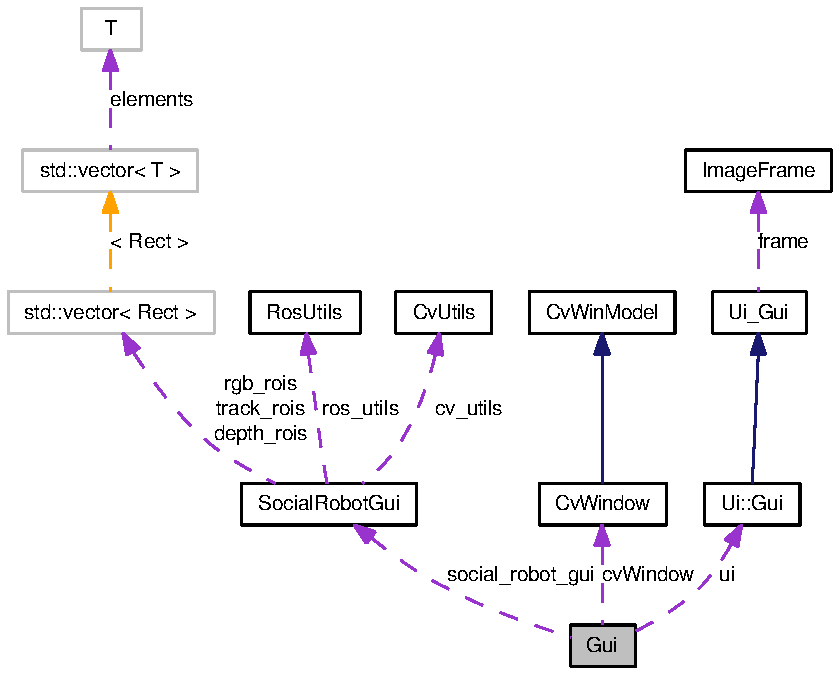
\includegraphics[width=400pt]{classGui__coll__graph}
\end{center}
\end{figure}
\subsection*{Public Member Functions}
\begin{DoxyCompactItemize}
\item 
\hyperlink{classGui_a797b7ddfe4c19abb19a37255de3eaefe}{Gui} (int argc, char $\ast$$\ast$argv, QWidget $\ast$parent=0)
\item 
\hyperlink{classGui_a4fd8485d226f9b8a2ac2d81d7f0f3598}{$\sim$Gui} ()
\end{DoxyCompactItemize}


\subsection{Constructor \& Destructor Documentation}
\hypertarget{classGui_a797b7ddfe4c19abb19a37255de3eaefe}{
\index{Gui@{Gui}!Gui@{Gui}}
\index{Gui@{Gui}!Gui@{Gui}}
\subsubsection[{Gui}]{\setlength{\rightskip}{0pt plus 5cm}Gui::Gui (int {\em argc}, \/  char $\ast$$\ast$ {\em argv}, \/  QWidget $\ast$ {\em parent} = {\ttfamily 0})\hspace{0.3cm}{\ttfamily  \mbox{[}explicit\mbox{]}}}}
\label{classGui_a797b7ddfe4c19abb19a37255de3eaefe}
\hypertarget{classGui_a4fd8485d226f9b8a2ac2d81d7f0f3598}{
\index{Gui@{Gui}!$\sim$Gui@{$\sim$Gui}}
\index{$\sim$Gui@{$\sim$Gui}!Gui@{Gui}}
\subsubsection[{$\sim$Gui}]{\setlength{\rightskip}{0pt plus 5cm}Gui::$\sim$Gui ()}}
\label{classGui_a4fd8485d226f9b8a2ac2d81d7f0f3598}


The documentation for this class was generated from the following files:\begin{DoxyCompactItemize}
\item 
\hyperlink{gui_8h}{gui.h}\item 
\hyperlink{gui_8cpp}{gui.cpp}\end{DoxyCompactItemize}

\hypertarget{classGuiReceiver}{
\section{GuiReceiver Class Reference}
\label{classGuiReceiver}\index{GuiReceiver@{GuiReceiver}}
}


{\ttfamily \#include $<$window\_\-QT.h$>$}

\subsection*{Public Slots}
\begin{DoxyCompactItemize}
\item 
void \hyperlink{classGuiReceiver_a59873b996659d0bb92d09638902ec4dc}{createWindow} (QString name, int flags=0)
\item 
void \hyperlink{classGuiReceiver_a86942e372e278c27c98af1930d9b9e97}{destroyWindow} (QString name)
\item 
void \hyperlink{classGuiReceiver_a748313239bdf5a50cc877dd91b3c1950}{destroyAllWindow} ()
\item 
void \hyperlink{classGuiReceiver_a8bd54a4f6d6f56083c2146173be6a1e3}{addSlider} (QString trackbar\_\-name, QString window\_\-name, void $\ast$value, int count, void $\ast$on\_\-change)
\item 
void \hyperlink{classGuiReceiver_a02ddc77f4583508363df717fd0859786}{addSlider2} (QString trackbar\_\-name, QString window\_\-name, void $\ast$value, int count, void $\ast$on\_\-change, void $\ast$userdata)
\item 
void \hyperlink{classGuiReceiver_abb7e0a41c2db119bfd76906651feb5aa}{moveWindow} (QString name, int x, int y)
\item 
void \hyperlink{classGuiReceiver_a42b8802376fe8f63922969475875eea6}{resizeWindow} (QString name, int width, int height)
\item 
void \hyperlink{classGuiReceiver_a185d6468377d45e2a2589bbb64a9ec62}{showImage} (QString name, void $\ast$arr)
\item 
void \hyperlink{classGuiReceiver_a1e010c3db9ebaaf1efddb8c03f558e88}{displayInfo} (QString name, QString text, int delayms)
\item 
void \hyperlink{classGuiReceiver_abfc7c7fb831a8c423a7a15e2b0ec994b}{displayStatusBar} (QString name, QString text, int delayms)
\item 
void \hyperlink{classGuiReceiver_aa8aab548c6a8fb1463c6cc7eb133ce7c}{timeOut} ()
\item 
void \hyperlink{classGuiReceiver_a50571c44603479d7d96426b1de23b010}{toggleFullScreen} (QString name, double flags)
\item 
double \hyperlink{classGuiReceiver_a6dd924ef78d8e7ec9e008f9007dbd032}{isFullScreen} (QString name)
\item 
double \hyperlink{classGuiReceiver_aff1aa23d540c06006c295ce69c8bb771}{getPropWindow} (QString name)
\item 
void \hyperlink{classGuiReceiver_a2f7df93bb22ec310b8f9b44844662b85}{setPropWindow} (QString name, double flags)
\item 
double \hyperlink{classGuiReceiver_aaf16c278a39a4ee6a02de8de5e348c5c}{getRatioWindow} (QString name)
\item 
void \hyperlink{classGuiReceiver_a42057f63804bb4f378c9ecb9a77f140c}{setRatioWindow} (QString name, double arg2)
\item 
void \hyperlink{classGuiReceiver_a0b4cb6c25ca109fdbcdc0538caf91da5}{saveWindowParameters} (QString name)
\item 
void \hyperlink{classGuiReceiver_afc852e63d8d8e4158984d37a444927ee}{loadWindowParameters} (QString name)
\item 
void \hyperlink{classGuiReceiver_a9d6fca288ed9086e22ad5d85ef0a3ae3}{putText} (void $\ast$arg1, QString text, QPoint org, void $\ast$font)
\item 
void \hyperlink{classGuiReceiver_aa1507b4023e4881e37c4b2a2ba0c2353}{addButton} (QString button\_\-name, int button\_\-type, int initial\_\-button\_\-state, void $\ast$on\_\-change, void $\ast$userdata)
\item 
void \hyperlink{classGuiReceiver_ad4c4385d49e830263e996416e16d137a}{enablePropertiesButtonEachWindow} ()
\end{DoxyCompactItemize}
\subsection*{Public Member Functions}
\begin{DoxyCompactItemize}
\item 
\hyperlink{classGuiReceiver_a0f840f04f1834a394fceeeca7dd88827}{GuiReceiver} ()
\item 
\hyperlink{classGuiReceiver_a7655140d1defb2adb481eab40193fd97}{$\sim$GuiReceiver} ()
\item 
int \hyperlink{classGuiReceiver_a4f0ca1781d324a9b658b01034895e1ee}{start} ()
\item 
void \hyperlink{classGuiReceiver_a9f788023836b17e8aed97b3770386ea9}{isLastWindow} ()
\end{DoxyCompactItemize}
\subsection*{Data Fields}
\begin{DoxyCompactItemize}
\item 
bool \hyperlink{classGuiReceiver_ad2d629b90a37e814db074e7ba1fc1aa9}{\_\-bTimeOut}
\item 
QTimer $\ast$ \hyperlink{classGuiReceiver_aeb64966586c4a35cfc02db46491afdf6}{timer}
\end{DoxyCompactItemize}


\subsection{Constructor \& Destructor Documentation}
\hypertarget{classGuiReceiver_a0f840f04f1834a394fceeeca7dd88827}{
\index{GuiReceiver@{GuiReceiver}!GuiReceiver@{GuiReceiver}}
\index{GuiReceiver@{GuiReceiver}!GuiReceiver@{GuiReceiver}}
\subsubsection[{GuiReceiver}]{\setlength{\rightskip}{0pt plus 5cm}GuiReceiver::GuiReceiver ()}}
\label{classGuiReceiver_a0f840f04f1834a394fceeeca7dd88827}
\hypertarget{classGuiReceiver_a7655140d1defb2adb481eab40193fd97}{
\index{GuiReceiver@{GuiReceiver}!$\sim$GuiReceiver@{$\sim$GuiReceiver}}
\index{$\sim$GuiReceiver@{$\sim$GuiReceiver}!GuiReceiver@{GuiReceiver}}
\subsubsection[{$\sim$GuiReceiver}]{\setlength{\rightskip}{0pt plus 5cm}GuiReceiver::$\sim$GuiReceiver ()}}
\label{classGuiReceiver_a7655140d1defb2adb481eab40193fd97}


\subsection{Member Function Documentation}
\hypertarget{classGuiReceiver_aa1507b4023e4881e37c4b2a2ba0c2353}{
\index{GuiReceiver@{GuiReceiver}!addButton@{addButton}}
\index{addButton@{addButton}!GuiReceiver@{GuiReceiver}}
\subsubsection[{addButton}]{\setlength{\rightskip}{0pt plus 5cm}void GuiReceiver::addButton (QString {\em button\_\-name}, \/  int {\em button\_\-type}, \/  int {\em initial\_\-button\_\-state}, \/  void $\ast$ {\em on\_\-change}, \/  void $\ast$ {\em userdata})\hspace{0.3cm}{\ttfamily  \mbox{[}slot\mbox{]}}}}
\label{classGuiReceiver_aa1507b4023e4881e37c4b2a2ba0c2353}
\hypertarget{classGuiReceiver_a8bd54a4f6d6f56083c2146173be6a1e3}{
\index{GuiReceiver@{GuiReceiver}!addSlider@{addSlider}}
\index{addSlider@{addSlider}!GuiReceiver@{GuiReceiver}}
\subsubsection[{addSlider}]{\setlength{\rightskip}{0pt plus 5cm}void GuiReceiver::addSlider (QString {\em trackbar\_\-name}, \/  QString {\em window\_\-name}, \/  void $\ast$ {\em value}, \/  int {\em count}, \/  void $\ast$ {\em on\_\-change})\hspace{0.3cm}{\ttfamily  \mbox{[}slot\mbox{]}}}}
\label{classGuiReceiver_a8bd54a4f6d6f56083c2146173be6a1e3}
\hypertarget{classGuiReceiver_a02ddc77f4583508363df717fd0859786}{
\index{GuiReceiver@{GuiReceiver}!addSlider2@{addSlider2}}
\index{addSlider2@{addSlider2}!GuiReceiver@{GuiReceiver}}
\subsubsection[{addSlider2}]{\setlength{\rightskip}{0pt plus 5cm}void GuiReceiver::addSlider2 (QString {\em trackbar\_\-name}, \/  QString {\em window\_\-name}, \/  void $\ast$ {\em value}, \/  int {\em count}, \/  void $\ast$ {\em on\_\-change}, \/  void $\ast$ {\em userdata})\hspace{0.3cm}{\ttfamily  \mbox{[}slot\mbox{]}}}}
\label{classGuiReceiver_a02ddc77f4583508363df717fd0859786}
\hypertarget{classGuiReceiver_a59873b996659d0bb92d09638902ec4dc}{
\index{GuiReceiver@{GuiReceiver}!createWindow@{createWindow}}
\index{createWindow@{createWindow}!GuiReceiver@{GuiReceiver}}
\subsubsection[{createWindow}]{\setlength{\rightskip}{0pt plus 5cm}void GuiReceiver::createWindow (QString {\em name}, \/  int {\em flags} = {\ttfamily 0})\hspace{0.3cm}{\ttfamily  \mbox{[}slot\mbox{]}}}}
\label{classGuiReceiver_a59873b996659d0bb92d09638902ec4dc}
\hypertarget{classGuiReceiver_a748313239bdf5a50cc877dd91b3c1950}{
\index{GuiReceiver@{GuiReceiver}!destroyAllWindow@{destroyAllWindow}}
\index{destroyAllWindow@{destroyAllWindow}!GuiReceiver@{GuiReceiver}}
\subsubsection[{destroyAllWindow}]{\setlength{\rightskip}{0pt plus 5cm}void GuiReceiver::destroyAllWindow ()\hspace{0.3cm}{\ttfamily  \mbox{[}slot\mbox{]}}}}
\label{classGuiReceiver_a748313239bdf5a50cc877dd91b3c1950}
\hypertarget{classGuiReceiver_a86942e372e278c27c98af1930d9b9e97}{
\index{GuiReceiver@{GuiReceiver}!destroyWindow@{destroyWindow}}
\index{destroyWindow@{destroyWindow}!GuiReceiver@{GuiReceiver}}
\subsubsection[{destroyWindow}]{\setlength{\rightskip}{0pt plus 5cm}void GuiReceiver::destroyWindow (QString {\em name})\hspace{0.3cm}{\ttfamily  \mbox{[}slot\mbox{]}}}}
\label{classGuiReceiver_a86942e372e278c27c98af1930d9b9e97}
\hypertarget{classGuiReceiver_a1e010c3db9ebaaf1efddb8c03f558e88}{
\index{GuiReceiver@{GuiReceiver}!displayInfo@{displayInfo}}
\index{displayInfo@{displayInfo}!GuiReceiver@{GuiReceiver}}
\subsubsection[{displayInfo}]{\setlength{\rightskip}{0pt plus 5cm}void GuiReceiver::displayInfo (QString {\em name}, \/  QString {\em text}, \/  int {\em delayms})\hspace{0.3cm}{\ttfamily  \mbox{[}slot\mbox{]}}}}
\label{classGuiReceiver_a1e010c3db9ebaaf1efddb8c03f558e88}
\hypertarget{classGuiReceiver_abfc7c7fb831a8c423a7a15e2b0ec994b}{
\index{GuiReceiver@{GuiReceiver}!displayStatusBar@{displayStatusBar}}
\index{displayStatusBar@{displayStatusBar}!GuiReceiver@{GuiReceiver}}
\subsubsection[{displayStatusBar}]{\setlength{\rightskip}{0pt plus 5cm}void GuiReceiver::displayStatusBar (QString {\em name}, \/  QString {\em text}, \/  int {\em delayms})\hspace{0.3cm}{\ttfamily  \mbox{[}slot\mbox{]}}}}
\label{classGuiReceiver_abfc7c7fb831a8c423a7a15e2b0ec994b}
\hypertarget{classGuiReceiver_ad4c4385d49e830263e996416e16d137a}{
\index{GuiReceiver@{GuiReceiver}!enablePropertiesButtonEachWindow@{enablePropertiesButtonEachWindow}}
\index{enablePropertiesButtonEachWindow@{enablePropertiesButtonEachWindow}!GuiReceiver@{GuiReceiver}}
\subsubsection[{enablePropertiesButtonEachWindow}]{\setlength{\rightskip}{0pt plus 5cm}void GuiReceiver::enablePropertiesButtonEachWindow ()\hspace{0.3cm}{\ttfamily  \mbox{[}slot\mbox{]}}}}
\label{classGuiReceiver_ad4c4385d49e830263e996416e16d137a}
\hypertarget{classGuiReceiver_aff1aa23d540c06006c295ce69c8bb771}{
\index{GuiReceiver@{GuiReceiver}!getPropWindow@{getPropWindow}}
\index{getPropWindow@{getPropWindow}!GuiReceiver@{GuiReceiver}}
\subsubsection[{getPropWindow}]{\setlength{\rightskip}{0pt plus 5cm}double GuiReceiver::getPropWindow (QString {\em name})\hspace{0.3cm}{\ttfamily  \mbox{[}slot\mbox{]}}}}
\label{classGuiReceiver_aff1aa23d540c06006c295ce69c8bb771}
\hypertarget{classGuiReceiver_aaf16c278a39a4ee6a02de8de5e348c5c}{
\index{GuiReceiver@{GuiReceiver}!getRatioWindow@{getRatioWindow}}
\index{getRatioWindow@{getRatioWindow}!GuiReceiver@{GuiReceiver}}
\subsubsection[{getRatioWindow}]{\setlength{\rightskip}{0pt plus 5cm}double GuiReceiver::getRatioWindow (QString {\em name})\hspace{0.3cm}{\ttfamily  \mbox{[}slot\mbox{]}}}}
\label{classGuiReceiver_aaf16c278a39a4ee6a02de8de5e348c5c}
\hypertarget{classGuiReceiver_a6dd924ef78d8e7ec9e008f9007dbd032}{
\index{GuiReceiver@{GuiReceiver}!isFullScreen@{isFullScreen}}
\index{isFullScreen@{isFullScreen}!GuiReceiver@{GuiReceiver}}
\subsubsection[{isFullScreen}]{\setlength{\rightskip}{0pt plus 5cm}double GuiReceiver::isFullScreen (QString {\em name})\hspace{0.3cm}{\ttfamily  \mbox{[}slot\mbox{]}}}}
\label{classGuiReceiver_a6dd924ef78d8e7ec9e008f9007dbd032}
\hypertarget{classGuiReceiver_a9f788023836b17e8aed97b3770386ea9}{
\index{GuiReceiver@{GuiReceiver}!isLastWindow@{isLastWindow}}
\index{isLastWindow@{isLastWindow}!GuiReceiver@{GuiReceiver}}
\subsubsection[{isLastWindow}]{\setlength{\rightskip}{0pt plus 5cm}void GuiReceiver::isLastWindow ()}}
\label{classGuiReceiver_a9f788023836b17e8aed97b3770386ea9}
\hypertarget{classGuiReceiver_afc852e63d8d8e4158984d37a444927ee}{
\index{GuiReceiver@{GuiReceiver}!loadWindowParameters@{loadWindowParameters}}
\index{loadWindowParameters@{loadWindowParameters}!GuiReceiver@{GuiReceiver}}
\subsubsection[{loadWindowParameters}]{\setlength{\rightskip}{0pt plus 5cm}void GuiReceiver::loadWindowParameters (QString {\em name})\hspace{0.3cm}{\ttfamily  \mbox{[}slot\mbox{]}}}}
\label{classGuiReceiver_afc852e63d8d8e4158984d37a444927ee}
\hypertarget{classGuiReceiver_abb7e0a41c2db119bfd76906651feb5aa}{
\index{GuiReceiver@{GuiReceiver}!moveWindow@{moveWindow}}
\index{moveWindow@{moveWindow}!GuiReceiver@{GuiReceiver}}
\subsubsection[{moveWindow}]{\setlength{\rightskip}{0pt plus 5cm}void GuiReceiver::moveWindow (QString {\em name}, \/  int {\em x}, \/  int {\em y})\hspace{0.3cm}{\ttfamily  \mbox{[}slot\mbox{]}}}}
\label{classGuiReceiver_abb7e0a41c2db119bfd76906651feb5aa}
\hypertarget{classGuiReceiver_a9d6fca288ed9086e22ad5d85ef0a3ae3}{
\index{GuiReceiver@{GuiReceiver}!putText@{putText}}
\index{putText@{putText}!GuiReceiver@{GuiReceiver}}
\subsubsection[{putText}]{\setlength{\rightskip}{0pt plus 5cm}void GuiReceiver::putText (void $\ast$ {\em arg1}, \/  QString {\em text}, \/  QPoint {\em org}, \/  void $\ast$ {\em font})\hspace{0.3cm}{\ttfamily  \mbox{[}slot\mbox{]}}}}
\label{classGuiReceiver_a9d6fca288ed9086e22ad5d85ef0a3ae3}
\hypertarget{classGuiReceiver_a42b8802376fe8f63922969475875eea6}{
\index{GuiReceiver@{GuiReceiver}!resizeWindow@{resizeWindow}}
\index{resizeWindow@{resizeWindow}!GuiReceiver@{GuiReceiver}}
\subsubsection[{resizeWindow}]{\setlength{\rightskip}{0pt plus 5cm}void GuiReceiver::resizeWindow (QString {\em name}, \/  int {\em width}, \/  int {\em height})\hspace{0.3cm}{\ttfamily  \mbox{[}slot\mbox{]}}}}
\label{classGuiReceiver_a42b8802376fe8f63922969475875eea6}
\hypertarget{classGuiReceiver_a0b4cb6c25ca109fdbcdc0538caf91da5}{
\index{GuiReceiver@{GuiReceiver}!saveWindowParameters@{saveWindowParameters}}
\index{saveWindowParameters@{saveWindowParameters}!GuiReceiver@{GuiReceiver}}
\subsubsection[{saveWindowParameters}]{\setlength{\rightskip}{0pt plus 5cm}void GuiReceiver::saveWindowParameters (QString {\em name})\hspace{0.3cm}{\ttfamily  \mbox{[}slot\mbox{]}}}}
\label{classGuiReceiver_a0b4cb6c25ca109fdbcdc0538caf91da5}
\hypertarget{classGuiReceiver_a2f7df93bb22ec310b8f9b44844662b85}{
\index{GuiReceiver@{GuiReceiver}!setPropWindow@{setPropWindow}}
\index{setPropWindow@{setPropWindow}!GuiReceiver@{GuiReceiver}}
\subsubsection[{setPropWindow}]{\setlength{\rightskip}{0pt plus 5cm}void GuiReceiver::setPropWindow (QString {\em name}, \/  double {\em flags})\hspace{0.3cm}{\ttfamily  \mbox{[}slot\mbox{]}}}}
\label{classGuiReceiver_a2f7df93bb22ec310b8f9b44844662b85}
\hypertarget{classGuiReceiver_a42057f63804bb4f378c9ecb9a77f140c}{
\index{GuiReceiver@{GuiReceiver}!setRatioWindow@{setRatioWindow}}
\index{setRatioWindow@{setRatioWindow}!GuiReceiver@{GuiReceiver}}
\subsubsection[{setRatioWindow}]{\setlength{\rightskip}{0pt plus 5cm}void GuiReceiver::setRatioWindow (QString {\em name}, \/  double {\em arg2})\hspace{0.3cm}{\ttfamily  \mbox{[}slot\mbox{]}}}}
\label{classGuiReceiver_a42057f63804bb4f378c9ecb9a77f140c}
\hypertarget{classGuiReceiver_a185d6468377d45e2a2589bbb64a9ec62}{
\index{GuiReceiver@{GuiReceiver}!showImage@{showImage}}
\index{showImage@{showImage}!GuiReceiver@{GuiReceiver}}
\subsubsection[{showImage}]{\setlength{\rightskip}{0pt plus 5cm}void GuiReceiver::showImage (QString {\em name}, \/  void $\ast$ {\em arr})\hspace{0.3cm}{\ttfamily  \mbox{[}slot\mbox{]}}}}
\label{classGuiReceiver_a185d6468377d45e2a2589bbb64a9ec62}
\hypertarget{classGuiReceiver_a4f0ca1781d324a9b658b01034895e1ee}{
\index{GuiReceiver@{GuiReceiver}!start@{start}}
\index{start@{start}!GuiReceiver@{GuiReceiver}}
\subsubsection[{start}]{\setlength{\rightskip}{0pt plus 5cm}int GuiReceiver::start ()}}
\label{classGuiReceiver_a4f0ca1781d324a9b658b01034895e1ee}
\hypertarget{classGuiReceiver_aa8aab548c6a8fb1463c6cc7eb133ce7c}{
\index{GuiReceiver@{GuiReceiver}!timeOut@{timeOut}}
\index{timeOut@{timeOut}!GuiReceiver@{GuiReceiver}}
\subsubsection[{timeOut}]{\setlength{\rightskip}{0pt plus 5cm}void GuiReceiver::timeOut ()\hspace{0.3cm}{\ttfamily  \mbox{[}slot\mbox{]}}}}
\label{classGuiReceiver_aa8aab548c6a8fb1463c6cc7eb133ce7c}
\hypertarget{classGuiReceiver_a50571c44603479d7d96426b1de23b010}{
\index{GuiReceiver@{GuiReceiver}!toggleFullScreen@{toggleFullScreen}}
\index{toggleFullScreen@{toggleFullScreen}!GuiReceiver@{GuiReceiver}}
\subsubsection[{toggleFullScreen}]{\setlength{\rightskip}{0pt plus 5cm}void GuiReceiver::toggleFullScreen (QString {\em name}, \/  double {\em flags})\hspace{0.3cm}{\ttfamily  \mbox{[}slot\mbox{]}}}}
\label{classGuiReceiver_a50571c44603479d7d96426b1de23b010}


\subsection{Field Documentation}
\hypertarget{classGuiReceiver_ad2d629b90a37e814db074e7ba1fc1aa9}{
\index{GuiReceiver@{GuiReceiver}!\_\-bTimeOut@{\_\-bTimeOut}}
\index{\_\-bTimeOut@{\_\-bTimeOut}!GuiReceiver@{GuiReceiver}}
\subsubsection[{\_\-bTimeOut}]{\setlength{\rightskip}{0pt plus 5cm}bool {\bf GuiReceiver::\_\-bTimeOut}}}
\label{classGuiReceiver_ad2d629b90a37e814db074e7ba1fc1aa9}
\hypertarget{classGuiReceiver_aeb64966586c4a35cfc02db46491afdf6}{
\index{GuiReceiver@{GuiReceiver}!timer@{timer}}
\index{timer@{timer}!GuiReceiver@{GuiReceiver}}
\subsubsection[{timer}]{\setlength{\rightskip}{0pt plus 5cm}QTimer$\ast$ {\bf GuiReceiver::timer}}}
\label{classGuiReceiver_aeb64966586c4a35cfc02db46491afdf6}


The documentation for this class was generated from the following files:\begin{DoxyCompactItemize}
\item 
\hyperlink{window__QT_8h}{window\_\-QT.h}\item 
\hyperlink{window__QT_8cpp}{window\_\-QT.cpp}\end{DoxyCompactItemize}

\hypertarget{classImageFrame}{\section{Image\-Frame Class Reference}
\label{classImageFrame}\index{Image\-Frame@{Image\-Frame}}
}


{\ttfamily \#include $<$imageframe.\-h$>$}



Inheritance diagram for Image\-Frame\-:\nopagebreak
\begin{figure}[H]
\begin{center}
\leavevmode
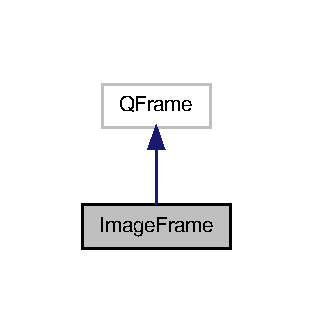
\includegraphics[width=150pt]{classImageFrame__inherit__graph}
\end{center}
\end{figure}


Collaboration diagram for Image\-Frame\-:\nopagebreak
\begin{figure}[H]
\begin{center}
\leavevmode
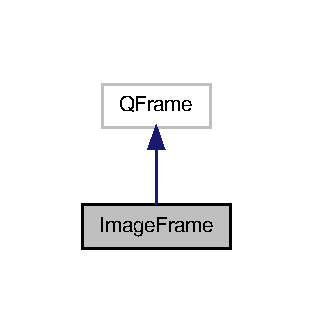
\includegraphics[width=150pt]{classImageFrame__coll__graph}
\end{center}
\end{figure}
\subsection*{Public Slots}
\begin{DoxyCompactItemize}
\item 
void \hyperlink{classImageFrame_a03c4a3c033846294a43a2a87eb0b5f30}{resize\-Event} (Q\-Resize\-Event $\ast$)
\end{DoxyCompactItemize}
\subsection*{Signals}
\begin{DoxyCompactItemize}
\item 
void \hyperlink{classImageFrame_afc5c795cc06bab2f82d286084dc8eb14}{resize\-Image} (Q\-Size new\-Size)
\end{DoxyCompactItemize}
\subsection*{Public Member Functions}
\begin{DoxyCompactItemize}
\item 
\hyperlink{classImageFrame_a4691aecc4a0685f30f18941b1354fe66}{Image\-Frame} (Q\-Widget $\ast$parent=0)
\end{DoxyCompactItemize}


\subsection{Constructor \& Destructor Documentation}
\hypertarget{classImageFrame_a4691aecc4a0685f30f18941b1354fe66}{\index{Image\-Frame@{Image\-Frame}!Image\-Frame@{Image\-Frame}}
\index{Image\-Frame@{Image\-Frame}!ImageFrame@{Image\-Frame}}
\subsubsection[{Image\-Frame}]{\setlength{\rightskip}{0pt plus 5cm}Image\-Frame\-::\-Image\-Frame (
\begin{DoxyParamCaption}
\item[{Q\-Widget $\ast$}]{parent = {\ttfamily 0}}
\end{DoxyParamCaption}
)\hspace{0.3cm}{\ttfamily [explicit]}}}\label{classImageFrame_a4691aecc4a0685f30f18941b1354fe66}


\subsection{Member Function Documentation}
\hypertarget{classImageFrame_a03c4a3c033846294a43a2a87eb0b5f30}{\index{Image\-Frame@{Image\-Frame}!resize\-Event@{resize\-Event}}
\index{resize\-Event@{resize\-Event}!ImageFrame@{Image\-Frame}}
\subsubsection[{resize\-Event}]{\setlength{\rightskip}{0pt plus 5cm}void Image\-Frame\-::resize\-Event (
\begin{DoxyParamCaption}
\item[{Q\-Resize\-Event $\ast$}]{event}
\end{DoxyParamCaption}
)\hspace{0.3cm}{\ttfamily [slot]}}}\label{classImageFrame_a03c4a3c033846294a43a2a87eb0b5f30}
\hypertarget{classImageFrame_afc5c795cc06bab2f82d286084dc8eb14}{\index{Image\-Frame@{Image\-Frame}!resize\-Image@{resize\-Image}}
\index{resize\-Image@{resize\-Image}!ImageFrame@{Image\-Frame}}
\subsubsection[{resize\-Image}]{\setlength{\rightskip}{0pt plus 5cm}void Image\-Frame\-::resize\-Image (
\begin{DoxyParamCaption}
\item[{Q\-Size}]{new\-Size}
\end{DoxyParamCaption}
)\hspace{0.3cm}{\ttfamily [signal]}}}\label{classImageFrame_afc5c795cc06bab2f82d286084dc8eb14}


The documentation for this class was generated from the following files\-:\begin{DoxyCompactItemize}
\item 
\hyperlink{imageframe_8h}{imageframe.\-h}\item 
\hyperlink{imageframe_8cpp}{imageframe.\-cpp}\end{DoxyCompactItemize}

\hypertarget{classParticleFilter}{\section{Particle\-Filter Class Reference}
\label{classParticleFilter}\index{Particle\-Filter@{Particle\-Filter}}
}


{\ttfamily \#include $<$filter.\-h$>$}



Inheritance diagram for Particle\-Filter\-:\nopagebreak
\begin{figure}[H]
\begin{center}
\leavevmode
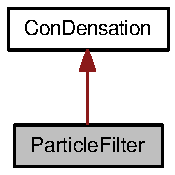
\includegraphics[width=158pt]{classParticleFilter__inherit__graph}
\end{center}
\end{figure}


Collaboration diagram for Particle\-Filter\-:\nopagebreak
\begin{figure}[H]
\begin{center}
\leavevmode
\includegraphics[width=302pt]{classParticleFilter__coll__graph}
\end{center}
\end{figure}
\subsection*{Public Types}
\begin{DoxyCompactItemize}
\item 
enum \hyperlink{classParticleFilter_a5fd916dcc074edfb45cf0f90e6e7816a}{Filter\-States} \{ \\*
\hyperlink{classParticleFilter_a5fd916dcc074edfb45cf0f90e6e7816aa592f65912830c1757e3dd87aaf094ded}{S\-T\-A\-T\-E\-\_\-\-X}, 
\hyperlink{classParticleFilter_a5fd916dcc074edfb45cf0f90e6e7816aaaccdf213f2315178644fa199657af377}{S\-T\-A\-T\-E\-\_\-\-Y}, 
\hyperlink{classParticleFilter_a5fd916dcc074edfb45cf0f90e6e7816aa8f405cfb59cb161e13f67ac80f048d64}{S\-T\-A\-T\-E\-\_\-\-X\-\_\-\-V\-E\-L}, 
\hyperlink{classParticleFilter_a5fd916dcc074edfb45cf0f90e6e7816aaa5c18829321e55f7f3ccbe9521160d43}{S\-T\-A\-T\-E\-\_\-\-Y\-\_\-\-V\-E\-L}, 
\\*
\hyperlink{classParticleFilter_a5fd916dcc074edfb45cf0f90e6e7816aac85f631868fa888a31c4b1048f26c9b9}{S\-T\-A\-T\-E\-\_\-\-S\-C\-A\-L\-E}, 
\hyperlink{classParticleFilter_a5fd916dcc074edfb45cf0f90e6e7816aa6be500dda12c848a8fa746cecf967e59}{N\-U\-M\-\_\-\-S\-T\-A\-T\-E\-S}
 \}
\end{DoxyCompactItemize}
\subsection*{Public Member Functions}
\begin{DoxyCompactItemize}
\item 
\hyperlink{classParticleFilter_a76dd2772cb2d4a3eece16415691bc39c}{Particle\-Filter} (int \hyperlink{social__robot_8cpp_acf574bc864f7f0fc111320f1d6c449d5}{num\-\_\-particles})
\item 
virtual \hyperlink{classParticleFilter_a4f4ccdfa224f0a62c411230f7fb0cd65}{$\sim$\-Particle\-Filter} ()
\item 
void \hyperlink{classParticleFilter_a06b39d5e76cbb5de792d7c1021c02557}{init} (const cv\-::\-Rect \&\hyperlink{social__robot__test_8cpp_a15633c47538e3790df1e008a7f6dbfea}{selection})
\item 
cv\-::\-Mat \& \hyperlink{classParticleFilter_a0903908806914466a41382242aadf466}{update} (cv\-::\-Mat \&\hyperlink{create__ground__truth_8cpp_aabb27b8973575043030df51be47cd24a}{image}, cv\-::\-Mat \&\hyperlink{social__robot__onethread_8cpp_a5b613972ff73fd7b34e0ee18acc5c1a6}{depth\-\_\-image}, const cv\-::\-Size \&target\-\_\-size, cv\-::\-Mat \&target\-\_\-hist, int hist\-\_\-type)
\item 
void \hyperlink{classParticleFilter_a93b28af3da883f2b1a8d662fe72ddb2b}{draw\-\_\-estimated\-\_\-state} (cv\-::\-Mat \&\hyperlink{create__ground__truth_8cpp_aabb27b8973575043030df51be47cd24a}{image}, const cv\-::\-Size \&target\-\_\-size, const cv\-::\-Scalar \&color)
\item 
void \hyperlink{classParticleFilter_aff7ddfc78e3b1e46e344603cfc4b0632}{draw\-\_\-particles} (cv\-::\-Mat \&\hyperlink{create__ground__truth_8cpp_aabb27b8973575043030df51be47cd24a}{image}, const cv\-::\-Size \&target\-\_\-size, const cv\-::\-Scalar \&color)
\item 
void \hyperlink{classParticleFilter_a7054878a2bed0544f0915b4eecc2ffca}{redistribute} (const float lower\-\_\-bound\mbox{[}$\,$\mbox{]}, const float upper\-\_\-bound\mbox{[}$\,$\mbox{]})
\item 
cv\-::\-Rect \hyperlink{classParticleFilter_a74680a952aac5da591c2854ede6fbbd7}{get\-\_\-estimated\-\_\-state} (void)
\item 
float \hyperlink{classParticleFilter_a7d3863cfb7922787bdfae897bf24a734}{get\-\_\-estimated\-\_\-scale} (void)
\item 
const cv\-::\-Mat \& \hyperlink{classParticleFilter_a4c909c7d4af1dd9ea2d06a568212e3dc}{state} () const 
\item 
float \hyperlink{classParticleFilter_aba8448793be2944625d91b2ca1a2af17}{confidence} () const 
\end{DoxyCompactItemize}
\subsection*{Additional Inherited Members}


\subsection{Detailed Description}
\begin{DoxyCopyright}{Copyright}

\end{DoxyCopyright}
Copyright 2012 Kevin Schluff

This program is free software\-: you can redistribute it and/or modify it under the terms of the G\-N\-U General Public License version 2, as published by the Free Software Foundation.

This program is distributed in the hope that it will be useful, but W\-I\-T\-H\-O\-U\-T A\-N\-Y W\-A\-R\-R\-A\-N\-T\-Y; without even the implied warranty of M\-E\-R\-C\-H\-A\-N\-T\-A\-B\-I\-L\-I\-T\-Y or F\-I\-T\-N\-E\-S\-S F\-O\-R A P\-A\-R\-T\-I\-C\-U\-L\-A\-R P\-U\-R\-P\-O\-S\-E. See the G\-N\-U General Public License for more details.

You should have received a copy of the G\-N\-U General Public License along with this program. If not, see \href{http://www.gnu.org/licenses/}{\tt http\-://www.\-gnu.\-org/licenses/}. 

\subsection{Member Enumeration Documentation}
\hypertarget{classParticleFilter_a5fd916dcc074edfb45cf0f90e6e7816a}{\index{Particle\-Filter@{Particle\-Filter}!Filter\-States@{Filter\-States}}
\index{Filter\-States@{Filter\-States}!ParticleFilter@{Particle\-Filter}}
\subsubsection[{Filter\-States}]{\setlength{\rightskip}{0pt plus 5cm}enum {\bf Particle\-Filter\-::\-Filter\-States}}}\label{classParticleFilter_a5fd916dcc074edfb45cf0f90e6e7816a}
\begin{Desc}
\item[Enumerator\-: ]\par
\begin{description}
\index{S\-T\-A\-T\-E\-\_\-\-X@{S\-T\-A\-T\-E\-\_\-\-X}!Particle\-Filter@{Particle\-Filter}}\index{Particle\-Filter@{Particle\-Filter}!S\-T\-A\-T\-E\-\_\-\-X@{S\-T\-A\-T\-E\-\_\-\-X}}\item[{\em 
\hypertarget{classParticleFilter_a5fd916dcc074edfb45cf0f90e6e7816aa592f65912830c1757e3dd87aaf094ded}{S\-T\-A\-T\-E\-\_\-\-X}\label{classParticleFilter_a5fd916dcc074edfb45cf0f90e6e7816aa592f65912830c1757e3dd87aaf094ded}
}]\index{S\-T\-A\-T\-E\-\_\-\-Y@{S\-T\-A\-T\-E\-\_\-\-Y}!Particle\-Filter@{Particle\-Filter}}\index{Particle\-Filter@{Particle\-Filter}!S\-T\-A\-T\-E\-\_\-\-Y@{S\-T\-A\-T\-E\-\_\-\-Y}}\item[{\em 
\hypertarget{classParticleFilter_a5fd916dcc074edfb45cf0f90e6e7816aaaccdf213f2315178644fa199657af377}{S\-T\-A\-T\-E\-\_\-\-Y}\label{classParticleFilter_a5fd916dcc074edfb45cf0f90e6e7816aaaccdf213f2315178644fa199657af377}
}]\index{S\-T\-A\-T\-E\-\_\-\-X\-\_\-\-V\-E\-L@{S\-T\-A\-T\-E\-\_\-\-X\-\_\-\-V\-E\-L}!Particle\-Filter@{Particle\-Filter}}\index{Particle\-Filter@{Particle\-Filter}!S\-T\-A\-T\-E\-\_\-\-X\-\_\-\-V\-E\-L@{S\-T\-A\-T\-E\-\_\-\-X\-\_\-\-V\-E\-L}}\item[{\em 
\hypertarget{classParticleFilter_a5fd916dcc074edfb45cf0f90e6e7816aa8f405cfb59cb161e13f67ac80f048d64}{S\-T\-A\-T\-E\-\_\-\-X\-\_\-\-V\-E\-L}\label{classParticleFilter_a5fd916dcc074edfb45cf0f90e6e7816aa8f405cfb59cb161e13f67ac80f048d64}
}]\index{S\-T\-A\-T\-E\-\_\-\-Y\-\_\-\-V\-E\-L@{S\-T\-A\-T\-E\-\_\-\-Y\-\_\-\-V\-E\-L}!Particle\-Filter@{Particle\-Filter}}\index{Particle\-Filter@{Particle\-Filter}!S\-T\-A\-T\-E\-\_\-\-Y\-\_\-\-V\-E\-L@{S\-T\-A\-T\-E\-\_\-\-Y\-\_\-\-V\-E\-L}}\item[{\em 
\hypertarget{classParticleFilter_a5fd916dcc074edfb45cf0f90e6e7816aaa5c18829321e55f7f3ccbe9521160d43}{S\-T\-A\-T\-E\-\_\-\-Y\-\_\-\-V\-E\-L}\label{classParticleFilter_a5fd916dcc074edfb45cf0f90e6e7816aaa5c18829321e55f7f3ccbe9521160d43}
}]\index{S\-T\-A\-T\-E\-\_\-\-S\-C\-A\-L\-E@{S\-T\-A\-T\-E\-\_\-\-S\-C\-A\-L\-E}!Particle\-Filter@{Particle\-Filter}}\index{Particle\-Filter@{Particle\-Filter}!S\-T\-A\-T\-E\-\_\-\-S\-C\-A\-L\-E@{S\-T\-A\-T\-E\-\_\-\-S\-C\-A\-L\-E}}\item[{\em 
\hypertarget{classParticleFilter_a5fd916dcc074edfb45cf0f90e6e7816aac85f631868fa888a31c4b1048f26c9b9}{S\-T\-A\-T\-E\-\_\-\-S\-C\-A\-L\-E}\label{classParticleFilter_a5fd916dcc074edfb45cf0f90e6e7816aac85f631868fa888a31c4b1048f26c9b9}
}]\index{N\-U\-M\-\_\-\-S\-T\-A\-T\-E\-S@{N\-U\-M\-\_\-\-S\-T\-A\-T\-E\-S}!Particle\-Filter@{Particle\-Filter}}\index{Particle\-Filter@{Particle\-Filter}!N\-U\-M\-\_\-\-S\-T\-A\-T\-E\-S@{N\-U\-M\-\_\-\-S\-T\-A\-T\-E\-S}}\item[{\em 
\hypertarget{classParticleFilter_a5fd916dcc074edfb45cf0f90e6e7816aa6be500dda12c848a8fa746cecf967e59}{N\-U\-M\-\_\-\-S\-T\-A\-T\-E\-S}\label{classParticleFilter_a5fd916dcc074edfb45cf0f90e6e7816aa6be500dda12c848a8fa746cecf967e59}
}]\end{description}
\end{Desc}



\subsection{Constructor \& Destructor Documentation}
\hypertarget{classParticleFilter_a76dd2772cb2d4a3eece16415691bc39c}{\index{Particle\-Filter@{Particle\-Filter}!Particle\-Filter@{Particle\-Filter}}
\index{Particle\-Filter@{Particle\-Filter}!ParticleFilter@{Particle\-Filter}}
\subsubsection[{Particle\-Filter}]{\setlength{\rightskip}{0pt plus 5cm}Particle\-Filter\-::\-Particle\-Filter (
\begin{DoxyParamCaption}
\item[{int}]{num\-\_\-particles}
\end{DoxyParamCaption}
)}}\label{classParticleFilter_a76dd2772cb2d4a3eece16415691bc39c}
\hypertarget{classParticleFilter_a4f4ccdfa224f0a62c411230f7fb0cd65}{\index{Particle\-Filter@{Particle\-Filter}!$\sim$\-Particle\-Filter@{$\sim$\-Particle\-Filter}}
\index{$\sim$\-Particle\-Filter@{$\sim$\-Particle\-Filter}!ParticleFilter@{Particle\-Filter}}
\subsubsection[{$\sim$\-Particle\-Filter}]{\setlength{\rightskip}{0pt plus 5cm}Particle\-Filter\-::$\sim$\-Particle\-Filter (
\begin{DoxyParamCaption}
{}
\end{DoxyParamCaption}
)\hspace{0.3cm}{\ttfamily [virtual]}}}\label{classParticleFilter_a4f4ccdfa224f0a62c411230f7fb0cd65}


\subsection{Member Function Documentation}
\hypertarget{classParticleFilter_aba8448793be2944625d91b2ca1a2af17}{\index{Particle\-Filter@{Particle\-Filter}!confidence@{confidence}}
\index{confidence@{confidence}!ParticleFilter@{Particle\-Filter}}
\subsubsection[{confidence}]{\setlength{\rightskip}{0pt plus 5cm}float Particle\-Filter\-::confidence (
\begin{DoxyParamCaption}
{}
\end{DoxyParamCaption}
) const\hspace{0.3cm}{\ttfamily [inline]}}}\label{classParticleFilter_aba8448793be2944625d91b2ca1a2af17}
\hypertarget{classParticleFilter_a93b28af3da883f2b1a8d662fe72ddb2b}{\index{Particle\-Filter@{Particle\-Filter}!draw\-\_\-estimated\-\_\-state@{draw\-\_\-estimated\-\_\-state}}
\index{draw\-\_\-estimated\-\_\-state@{draw\-\_\-estimated\-\_\-state}!ParticleFilter@{Particle\-Filter}}
\subsubsection[{draw\-\_\-estimated\-\_\-state}]{\setlength{\rightskip}{0pt plus 5cm}void Particle\-Filter\-::draw\-\_\-estimated\-\_\-state (
\begin{DoxyParamCaption}
\item[{cv\-::\-Mat \&}]{image, }
\item[{const cv\-::\-Size \&}]{target\-\_\-size, }
\item[{const cv\-::\-Scalar \&}]{color}
\end{DoxyParamCaption}
)}}\label{classParticleFilter_a93b28af3da883f2b1a8d662fe72ddb2b}
\hypertarget{classParticleFilter_aff7ddfc78e3b1e46e344603cfc4b0632}{\index{Particle\-Filter@{Particle\-Filter}!draw\-\_\-particles@{draw\-\_\-particles}}
\index{draw\-\_\-particles@{draw\-\_\-particles}!ParticleFilter@{Particle\-Filter}}
\subsubsection[{draw\-\_\-particles}]{\setlength{\rightskip}{0pt plus 5cm}void Particle\-Filter\-::draw\-\_\-particles (
\begin{DoxyParamCaption}
\item[{cv\-::\-Mat \&}]{image, }
\item[{const cv\-::\-Size \&}]{target\-\_\-size, }
\item[{const cv\-::\-Scalar \&}]{color}
\end{DoxyParamCaption}
)}}\label{classParticleFilter_aff7ddfc78e3b1e46e344603cfc4b0632}
\hypertarget{classParticleFilter_a7d3863cfb7922787bdfae897bf24a734}{\index{Particle\-Filter@{Particle\-Filter}!get\-\_\-estimated\-\_\-scale@{get\-\_\-estimated\-\_\-scale}}
\index{get\-\_\-estimated\-\_\-scale@{get\-\_\-estimated\-\_\-scale}!ParticleFilter@{Particle\-Filter}}
\subsubsection[{get\-\_\-estimated\-\_\-scale}]{\setlength{\rightskip}{0pt plus 5cm}float Particle\-Filter\-::get\-\_\-estimated\-\_\-scale (
\begin{DoxyParamCaption}
\item[{void}]{}
\end{DoxyParamCaption}
)}}\label{classParticleFilter_a7d3863cfb7922787bdfae897bf24a734}
\hypertarget{classParticleFilter_a74680a952aac5da591c2854ede6fbbd7}{\index{Particle\-Filter@{Particle\-Filter}!get\-\_\-estimated\-\_\-state@{get\-\_\-estimated\-\_\-state}}
\index{get\-\_\-estimated\-\_\-state@{get\-\_\-estimated\-\_\-state}!ParticleFilter@{Particle\-Filter}}
\subsubsection[{get\-\_\-estimated\-\_\-state}]{\setlength{\rightskip}{0pt plus 5cm}Rect Particle\-Filter\-::get\-\_\-estimated\-\_\-state (
\begin{DoxyParamCaption}
\item[{void}]{}
\end{DoxyParamCaption}
)}}\label{classParticleFilter_a74680a952aac5da591c2854ede6fbbd7}
\hypertarget{classParticleFilter_a06b39d5e76cbb5de792d7c1021c02557}{\index{Particle\-Filter@{Particle\-Filter}!init@{init}}
\index{init@{init}!ParticleFilter@{Particle\-Filter}}
\subsubsection[{init}]{\setlength{\rightskip}{0pt plus 5cm}void Particle\-Filter\-::init (
\begin{DoxyParamCaption}
\item[{const cv\-::\-Rect \&}]{selection}
\end{DoxyParamCaption}
)}}\label{classParticleFilter_a06b39d5e76cbb5de792d7c1021c02557}
\hypertarget{classParticleFilter_a7054878a2bed0544f0915b4eecc2ffca}{\index{Particle\-Filter@{Particle\-Filter}!redistribute@{redistribute}}
\index{redistribute@{redistribute}!ParticleFilter@{Particle\-Filter}}
\subsubsection[{redistribute}]{\setlength{\rightskip}{0pt plus 5cm}void Particle\-Filter\-::redistribute (
\begin{DoxyParamCaption}
\item[{const float}]{lower\-\_\-bound\mbox{[}$\,$\mbox{]}, }
\item[{const float}]{upper\-\_\-bound\mbox{[}$\,$\mbox{]}}
\end{DoxyParamCaption}
)}}\label{classParticleFilter_a7054878a2bed0544f0915b4eecc2ffca}
\hypertarget{classParticleFilter_a4c909c7d4af1dd9ea2d06a568212e3dc}{\index{Particle\-Filter@{Particle\-Filter}!state@{state}}
\index{state@{state}!ParticleFilter@{Particle\-Filter}}
\subsubsection[{state}]{\setlength{\rightskip}{0pt plus 5cm}const cv\-::\-Mat\& Particle\-Filter\-::state (
\begin{DoxyParamCaption}
{}
\end{DoxyParamCaption}
) const\hspace{0.3cm}{\ttfamily [inline]}}}\label{classParticleFilter_a4c909c7d4af1dd9ea2d06a568212e3dc}
\hypertarget{classParticleFilter_a0903908806914466a41382242aadf466}{\index{Particle\-Filter@{Particle\-Filter}!update@{update}}
\index{update@{update}!ParticleFilter@{Particle\-Filter}}
\subsubsection[{update}]{\setlength{\rightskip}{0pt plus 5cm}Mat \& Particle\-Filter\-::update (
\begin{DoxyParamCaption}
\item[{cv\-::\-Mat \&}]{image, }
\item[{cv\-::\-Mat \&}]{depth\-\_\-image, }
\item[{const cv\-::\-Size \&}]{target\-\_\-size, }
\item[{cv\-::\-Mat \&}]{target\-\_\-hist, }
\item[{int}]{hist\-\_\-type}
\end{DoxyParamCaption}
)}}\label{classParticleFilter_a0903908806914466a41382242aadf466}
Update filter with measurements and time step. 

The documentation for this class was generated from the following files\-:\begin{DoxyCompactItemize}
\item 
\hyperlink{filter_8h}{filter.\-h}\item 
\hyperlink{filter_8cpp}{filter.\-cpp}\end{DoxyCompactItemize}

\hypertarget{classPixelSimilarity}{
\section{PixelSimilarity Class Reference}
\label{classPixelSimilarity}\index{PixelSimilarity@{PixelSimilarity}}
}


This class provides the location, radius and likelihood of a given potential head.  




{\ttfamily \#include $<$PixelSimilarity.h$>$}

\subsection*{Public Member Functions}
\begin{DoxyCompactItemize}
\item 
\hyperlink{classPixelSimilarity_a8d2c663a253dafb804765764e2dea32a}{PixelSimilarity} ()
\item 
\hyperlink{classPixelSimilarity_a0816faaaedb8d0e1ffe0aa40a438df4e}{PixelSimilarity} (cv::Point \hyperlink{classPixelSimilarity_a98e029104a5ee11b23554b02d7ac30e6}{point}, float \hyperlink{classPixelSimilarity_a4da3847fd0812a4c4fc415a20697acf4}{radius}, float \hyperlink{classPixelSimilarity_a4fa484885e6d7d38078c6d75e4f4d72e}{similarity})
\end{DoxyCompactItemize}
\subsection*{Data Fields}
\begin{DoxyCompactItemize}
\item 
cv::Point \hyperlink{classPixelSimilarity_a98e029104a5ee11b23554b02d7ac30e6}{point}
\item 
float \hyperlink{classPixelSimilarity_a4da3847fd0812a4c4fc415a20697acf4}{radius}
\item 
float \hyperlink{classPixelSimilarity_a4fa484885e6d7d38078c6d75e4f4d72e}{similarity}
\end{DoxyCompactItemize}


\subsection{Detailed Description}
This class provides the location, radius and likelihood of a given potential head. \begin{DoxyAuthor}{Author}
Social Robot 
\end{DoxyAuthor}


\subsection{Constructor \& Destructor Documentation}
\hypertarget{classPixelSimilarity_a8d2c663a253dafb804765764e2dea32a}{
\index{PixelSimilarity@{PixelSimilarity}!PixelSimilarity@{PixelSimilarity}}
\index{PixelSimilarity@{PixelSimilarity}!PixelSimilarity@{PixelSimilarity}}
\subsubsection[{PixelSimilarity}]{\setlength{\rightskip}{0pt plus 5cm}PixelSimilarity::PixelSimilarity ()}}
\label{classPixelSimilarity_a8d2c663a253dafb804765764e2dea32a}
Default Constructor. \hypertarget{classPixelSimilarity_a0816faaaedb8d0e1ffe0aa40a438df4e}{
\index{PixelSimilarity@{PixelSimilarity}!PixelSimilarity@{PixelSimilarity}}
\index{PixelSimilarity@{PixelSimilarity}!PixelSimilarity@{PixelSimilarity}}
\subsubsection[{PixelSimilarity}]{\setlength{\rightskip}{0pt plus 5cm}PixelSimilarity::PixelSimilarity (cv::Point {\em point}, \/  float {\em radius}, \/  float {\em similarity})}}
\label{classPixelSimilarity_a0816faaaedb8d0e1ffe0aa40a438df4e}
Constructor given location, radius and likelihood. 
\begin{DoxyParams}{Parameters}
\item[{\em point}]A point containing the x and y coordinates. \item[{\em radius}]A float for the radius of the head in pixels. \item[{\em similarity}]A float between 0 and 1 for the likelihood. \end{DoxyParams}


\subsection{Field Documentation}
\hypertarget{classPixelSimilarity_a98e029104a5ee11b23554b02d7ac30e6}{
\index{PixelSimilarity@{PixelSimilarity}!point@{point}}
\index{point@{point}!PixelSimilarity@{PixelSimilarity}}
\subsubsection[{point}]{\setlength{\rightskip}{0pt plus 5cm}cv::Point {\bf PixelSimilarity::point}}}
\label{classPixelSimilarity_a98e029104a5ee11b23554b02d7ac30e6}
\hypertarget{classPixelSimilarity_a4da3847fd0812a4c4fc415a20697acf4}{
\index{PixelSimilarity@{PixelSimilarity}!radius@{radius}}
\index{radius@{radius}!PixelSimilarity@{PixelSimilarity}}
\subsubsection[{radius}]{\setlength{\rightskip}{0pt plus 5cm}float {\bf PixelSimilarity::radius}}}
\label{classPixelSimilarity_a4da3847fd0812a4c4fc415a20697acf4}
\hypertarget{classPixelSimilarity_a4fa484885e6d7d38078c6d75e4f4d72e}{
\index{PixelSimilarity@{PixelSimilarity}!similarity@{similarity}}
\index{similarity@{similarity}!PixelSimilarity@{PixelSimilarity}}
\subsubsection[{similarity}]{\setlength{\rightskip}{0pt plus 5cm}float {\bf PixelSimilarity::similarity}}}
\label{classPixelSimilarity_a4fa484885e6d7d38078c6d75e4f4d72e}


The documentation for this class was generated from the following files:\begin{DoxyCompactItemize}
\item 
\hyperlink{PixelSimilarity_8h}{PixelSimilarity.h}\item 
\hyperlink{PixelSimilarity_8cpp}{PixelSimilarity.cpp}\end{DoxyCompactItemize}

\hypertarget{classsocial__robot_1_1msg_1_1__RegionOfInterests_1_1RegionOfInterests}{
\section{social\_\-robot::msg::\_\-RegionOfInterests::RegionOfInterests Class Reference}
\label{classsocial__robot_1_1msg_1_1__RegionOfInterests_1_1RegionOfInterests}\index{social\_\-robot::msg::\_\-RegionOfInterests::RegionOfInterests@{social\_\-robot::msg::\_\-RegionOfInterests::RegionOfInterests}}
}
\subsection*{Public Member Functions}
\begin{DoxyCompactItemize}
\item 
def \hyperlink{classsocial__robot_1_1msg_1_1__RegionOfInterests_1_1RegionOfInterests_a2db171c12bf93b29f41111a5ff1c2fc8}{\_\-\_\-init\_\-\_\-}
\item 
def \hyperlink{classsocial__robot_1_1msg_1_1__RegionOfInterests_1_1RegionOfInterests_abb6d0b069ff1727aec6ded395d171a77}{serialize}
\item 
def \hyperlink{classsocial__robot_1_1msg_1_1__RegionOfInterests_1_1RegionOfInterests_a5991036e5324683608a95d0ffad57a0c}{deserialize}
\item 
def \hyperlink{classsocial__robot_1_1msg_1_1__RegionOfInterests_1_1RegionOfInterests_aa464213af4d39dd2ad1c1d52f91ea3a2}{serialize\_\-numpy}
\item 
def \hyperlink{classsocial__robot_1_1msg_1_1__RegionOfInterests_1_1RegionOfInterests_a6d25339da85ed702e19e3ccdeb88d360}{deserialize\_\-numpy}
\end{DoxyCompactItemize}
\subsection*{Data Fields}
\begin{DoxyCompactItemize}
\item 
\hyperlink{classsocial__robot_1_1msg_1_1__RegionOfInterests_1_1RegionOfInterests_a89d94e67422a005c044977474b332fef}{rois}
\end{DoxyCompactItemize}


\subsection{Member Function Documentation}
\hypertarget{classsocial__robot_1_1msg_1_1__RegionOfInterests_1_1RegionOfInterests_a2db171c12bf93b29f41111a5ff1c2fc8}{
\index{social\_\-robot::msg::\_\-RegionOfInterests::RegionOfInterests@{social\_\-robot::msg::\_\-RegionOfInterests::RegionOfInterests}!\_\-\_\-init\_\-\_\-@{\_\-\_\-init\_\-\_\-}}
\index{\_\-\_\-init\_\-\_\-@{\_\-\_\-init\_\-\_\-}!social_robot::msg::_RegionOfInterests::RegionOfInterests@{social\_\-robot::msg::\_\-RegionOfInterests::RegionOfInterests}}
\subsubsection[{\_\-\_\-init\_\-\_\-}]{\setlength{\rightskip}{0pt plus 5cm}def social\_\-robot::msg::\_\-RegionOfInterests::RegionOfInterests::\_\-\_\-init\_\-\_\- ( {\em self}, \/   {\em args}, \/   {\em kwds})}}
\label{classsocial__robot_1_1msg_1_1__RegionOfInterests_1_1RegionOfInterests_a2db171c12bf93b29f41111a5ff1c2fc8}
\begin{DoxyVerb}
Constructor. Any message fields that are implicitly/explicitly
set to None will be assigned a default value. The recommend
use is keyword arguments as this is more robust to future message
changes.  You cannot mix in-order arguments and keyword arguments.

The available fields are:
   rois

@param args: complete set of field values, in .msg order
@param kwds: use keyword arguments corresponding to message field names
to set specific fields. 
\end{DoxyVerb}
 \hypertarget{classsocial__robot_1_1msg_1_1__RegionOfInterests_1_1RegionOfInterests_a5991036e5324683608a95d0ffad57a0c}{
\index{social\_\-robot::msg::\_\-RegionOfInterests::RegionOfInterests@{social\_\-robot::msg::\_\-RegionOfInterests::RegionOfInterests}!deserialize@{deserialize}}
\index{deserialize@{deserialize}!social_robot::msg::_RegionOfInterests::RegionOfInterests@{social\_\-robot::msg::\_\-RegionOfInterests::RegionOfInterests}}
\subsubsection[{deserialize}]{\setlength{\rightskip}{0pt plus 5cm}def social\_\-robot::msg::\_\-RegionOfInterests::RegionOfInterests::deserialize ( {\em self}, \/   {\em str})}}
\label{classsocial__robot_1_1msg_1_1__RegionOfInterests_1_1RegionOfInterests_a5991036e5324683608a95d0ffad57a0c}
\begin{DoxyVerb}
unpack serialized message in str into this message instance
@param str: byte array of serialized message
@type  str: str
\end{DoxyVerb}
 \hypertarget{classsocial__robot_1_1msg_1_1__RegionOfInterests_1_1RegionOfInterests_a6d25339da85ed702e19e3ccdeb88d360}{
\index{social\_\-robot::msg::\_\-RegionOfInterests::RegionOfInterests@{social\_\-robot::msg::\_\-RegionOfInterests::RegionOfInterests}!deserialize\_\-numpy@{deserialize\_\-numpy}}
\index{deserialize\_\-numpy@{deserialize\_\-numpy}!social_robot::msg::_RegionOfInterests::RegionOfInterests@{social\_\-robot::msg::\_\-RegionOfInterests::RegionOfInterests}}
\subsubsection[{deserialize\_\-numpy}]{\setlength{\rightskip}{0pt plus 5cm}def social\_\-robot::msg::\_\-RegionOfInterests::RegionOfInterests::deserialize\_\-numpy ( {\em self}, \/   {\em str}, \/   {\em numpy})}}
\label{classsocial__robot_1_1msg_1_1__RegionOfInterests_1_1RegionOfInterests_a6d25339da85ed702e19e3ccdeb88d360}
\begin{DoxyVerb}
unpack serialized message in str into this message instance using numpy for array types
@param str: byte array of serialized message
@type  str: str
@param numpy: numpy python module
@type  numpy: module
\end{DoxyVerb}
 \hypertarget{classsocial__robot_1_1msg_1_1__RegionOfInterests_1_1RegionOfInterests_abb6d0b069ff1727aec6ded395d171a77}{
\index{social\_\-robot::msg::\_\-RegionOfInterests::RegionOfInterests@{social\_\-robot::msg::\_\-RegionOfInterests::RegionOfInterests}!serialize@{serialize}}
\index{serialize@{serialize}!social_robot::msg::_RegionOfInterests::RegionOfInterests@{social\_\-robot::msg::\_\-RegionOfInterests::RegionOfInterests}}
\subsubsection[{serialize}]{\setlength{\rightskip}{0pt plus 5cm}def social\_\-robot::msg::\_\-RegionOfInterests::RegionOfInterests::serialize ( {\em self}, \/   {\em buff})}}
\label{classsocial__robot_1_1msg_1_1__RegionOfInterests_1_1RegionOfInterests_abb6d0b069ff1727aec6ded395d171a77}
\begin{DoxyVerb}
serialize message into buffer
@param buff: buffer
@type  buff: StringIO
\end{DoxyVerb}
 \hypertarget{classsocial__robot_1_1msg_1_1__RegionOfInterests_1_1RegionOfInterests_aa464213af4d39dd2ad1c1d52f91ea3a2}{
\index{social\_\-robot::msg::\_\-RegionOfInterests::RegionOfInterests@{social\_\-robot::msg::\_\-RegionOfInterests::RegionOfInterests}!serialize\_\-numpy@{serialize\_\-numpy}}
\index{serialize\_\-numpy@{serialize\_\-numpy}!social_robot::msg::_RegionOfInterests::RegionOfInterests@{social\_\-robot::msg::\_\-RegionOfInterests::RegionOfInterests}}
\subsubsection[{serialize\_\-numpy}]{\setlength{\rightskip}{0pt plus 5cm}def social\_\-robot::msg::\_\-RegionOfInterests::RegionOfInterests::serialize\_\-numpy ( {\em self}, \/   {\em buff}, \/   {\em numpy})}}
\label{classsocial__robot_1_1msg_1_1__RegionOfInterests_1_1RegionOfInterests_aa464213af4d39dd2ad1c1d52f91ea3a2}
\begin{DoxyVerb}
serialize message with numpy array types into buffer
@param buff: buffer
@type  buff: StringIO
@param numpy: numpy python module
@type  numpy module
\end{DoxyVerb}
 

\subsection{Field Documentation}
\hypertarget{classsocial__robot_1_1msg_1_1__RegionOfInterests_1_1RegionOfInterests_a89d94e67422a005c044977474b332fef}{
\index{social\_\-robot::msg::\_\-RegionOfInterests::RegionOfInterests@{social\_\-robot::msg::\_\-RegionOfInterests::RegionOfInterests}!rois@{rois}}
\index{rois@{rois}!social_robot::msg::_RegionOfInterests::RegionOfInterests@{social\_\-robot::msg::\_\-RegionOfInterests::RegionOfInterests}}
\subsubsection[{rois}]{\setlength{\rightskip}{0pt plus 5cm}{\bf social\_\-robot::msg::\_\-RegionOfInterests::RegionOfInterests::rois}}}
\label{classsocial__robot_1_1msg_1_1__RegionOfInterests_1_1RegionOfInterests_a89d94e67422a005c044977474b332fef}


The documentation for this class was generated from the following file:\begin{DoxyCompactItemize}
\item 
\hyperlink{__RegionOfInterests_8py}{\_\-RegionOfInterests.py}\end{DoxyCompactItemize}

\hypertarget{classRosUtils}{
\section{RosUtils Class Reference}
\label{classRosUtils}\index{RosUtils@{RosUtils}}
}


This class is used for publishing the ouput rectangles in ROS.  




{\ttfamily \#include $<$RosUtils.h$>$}

\subsection*{Public Member Functions}
\begin{DoxyCompactItemize}
\item 
RegionOfInterest \hyperlink{classRosUtils_a14c90d8ff6c7a2eb6d030226cc19cf7e}{cvrect2rosroi} (Rect rect)
\item 
Rect \hyperlink{classRosUtils_af79ad6781024a9d081fdc8cf67782269}{rosroi2cvrect} (RegionOfInterest roi)
\item 
vector$<$ RegionOfInterest $>$ \hyperlink{classRosUtils_a10a6552d95ab7a6ee4122af4c4137523}{cvrects2rosrois} (vector$<$ Rect $>$ rects)
\item 
vector$<$ Rect $>$ \hyperlink{classRosUtils_aadb640f35f26394dfd6240b17c95c942}{rosrois2cvrects} (vector$<$ RegionOfInterest $>$ \hyperlink{social__robot__onethread_8cpp_acb84e343c5602756e13a851a44128639}{rois})
\end{DoxyCompactItemize}


\subsection{Detailed Description}
This class is used for publishing the ouput rectangles in ROS. \begin{DoxyAuthor}{Author}
Social Robot 
\end{DoxyAuthor}


\subsection{Member Function Documentation}
\hypertarget{classRosUtils_a14c90d8ff6c7a2eb6d030226cc19cf7e}{
\index{RosUtils@{RosUtils}!cvrect2rosroi@{cvrect2rosroi}}
\index{cvrect2rosroi@{cvrect2rosroi}!RosUtils@{RosUtils}}
\subsubsection[{cvrect2rosroi}]{\setlength{\rightskip}{0pt plus 5cm}RegionOfInterest RosUtils::cvrect2rosroi (Rect {\em rect})}}
\label{classRosUtils_a14c90d8ff6c7a2eb6d030226cc19cf7e}
This function returns a given rectangle in a regionofinterest used in ROS. \begin{DoxyReturn}{Returns}

\end{DoxyReturn}

\begin{DoxyParams}{Parameters}
\item[{\em template2d}]A Mat containing a binary image. \item[{\em template3d}]A Mat containing a grayscale image. Notice that template3d is a grayscale image, it is used 3d when the matching is done with the depth image. \end{DoxyParams}
\hypertarget{classRosUtils_a10a6552d95ab7a6ee4122af4c4137523}{
\index{RosUtils@{RosUtils}!cvrects2rosrois@{cvrects2rosrois}}
\index{cvrects2rosrois@{cvrects2rosrois}!RosUtils@{RosUtils}}
\subsubsection[{cvrects2rosrois}]{\setlength{\rightskip}{0pt plus 5cm}vector$<$ RegionOfInterest $>$ RosUtils::cvrects2rosrois (vector$<$ Rect $>$ {\em rects})}}
\label{classRosUtils_a10a6552d95ab7a6ee4122af4c4137523}
Constructor given 2D and 3D templates. 
\begin{DoxyParams}{Parameters}
\item[{\em template2d}]A Mat containing a binary image. \item[{\em template3d}]A Mat containing a grayscale image. Notice that template3d is a grayscale image, it is used 3d when the matching is done with the depth image. \end{DoxyParams}
\hypertarget{classRosUtils_af79ad6781024a9d081fdc8cf67782269}{
\index{RosUtils@{RosUtils}!rosroi2cvrect@{rosroi2cvrect}}
\index{rosroi2cvrect@{rosroi2cvrect}!RosUtils@{RosUtils}}
\subsubsection[{rosroi2cvrect}]{\setlength{\rightskip}{0pt plus 5cm}Rect RosUtils::rosroi2cvrect (RegionOfInterest {\em roi})}}
\label{classRosUtils_af79ad6781024a9d081fdc8cf67782269}
Constructor given 2D and 3D templates. 
\begin{DoxyParams}{Parameters}
\item[{\em template2d}]A Mat containing a binary image. \item[{\em template3d}]A Mat containing a grayscale image. Notice that template3d is a grayscale image, it is used 3d when the matching is done with the depth image. \end{DoxyParams}
\hypertarget{classRosUtils_aadb640f35f26394dfd6240b17c95c942}{
\index{RosUtils@{RosUtils}!rosrois2cvrects@{rosrois2cvrects}}
\index{rosrois2cvrects@{rosrois2cvrects}!RosUtils@{RosUtils}}
\subsubsection[{rosrois2cvrects}]{\setlength{\rightskip}{0pt plus 5cm}vector$<$ Rect $>$ RosUtils::rosrois2cvrects (vector$<$ RegionOfInterest $>$ {\em rois})}}
\label{classRosUtils_aadb640f35f26394dfd6240b17c95c942}
Constructor given 2D and 3D templates. 
\begin{DoxyParams}{Parameters}
\item[{\em template2d}]A Mat containing a binary image. \item[{\em template3d}]A Mat containing a grayscale image. Notice that template3d is a grayscale image, it is used 3d when the matching is done with the depth image. \end{DoxyParams}


The documentation for this class was generated from the following files:\begin{DoxyCompactItemize}
\item 
\hyperlink{RosUtils_8h}{RosUtils.h}\item 
\hyperlink{RosUtils_8cpp}{RosUtils.cpp}\end{DoxyCompactItemize}

\hypertarget{classSettings}{\section{Settings Class Reference}
\label{classSettings}\index{Settings@{Settings}}
}


Collaboration diagram for Settings\-:
\nopagebreak
\begin{figure}[H]
\begin{center}
\leavevmode
\includegraphics[width=294pt]{classSettings__coll__graph}
\end{center}
\end{figure}
\subsection*{Public Types}
\begin{DoxyCompactItemize}
\item 
enum \hyperlink{classSettings_a0e7117abd9427a6f8bc1d1d8d456b5c8}{Pattern} \{ \hyperlink{classSettings_a0e7117abd9427a6f8bc1d1d8d456b5c8ad2f421ce100bd7e0302b17bda1a74eb9}{N\-O\-T\-\_\-\-E\-X\-I\-S\-T\-I\-N\-G}, 
\hyperlink{classSettings_a0e7117abd9427a6f8bc1d1d8d456b5c8ae96aa2d60b4a554a215524a05b32908e}{C\-H\-E\-S\-S\-B\-O\-A\-R\-D}, 
\hyperlink{classSettings_a0e7117abd9427a6f8bc1d1d8d456b5c8a79472d1c69f8ed7aa1b55f908b136f68}{C\-I\-R\-C\-L\-E\-S\-\_\-\-G\-R\-I\-D}, 
\hyperlink{classSettings_a0e7117abd9427a6f8bc1d1d8d456b5c8a2cea29ee5896f2cb4cc64df25fd2375b}{A\-S\-Y\-M\-M\-E\-T\-R\-I\-C\-\_\-\-C\-I\-R\-C\-L\-E\-S\-\_\-\-G\-R\-I\-D}
 \}
\item 
enum \hyperlink{classSettings_a5afe85d24b071973a7f248c05386f7f4}{Input\-Type} \{ \hyperlink{classSettings_a5afe85d24b071973a7f248c05386f7f4adb44130895aedc32a119565eb6d61bed}{I\-N\-V\-A\-L\-I\-D}, 
\hyperlink{classSettings_a5afe85d24b071973a7f248c05386f7f4aba4cc7726878c8913831f0ea6360fa05}{C\-A\-M\-E\-R\-A}, 
\hyperlink{classSettings_a5afe85d24b071973a7f248c05386f7f4ac9fd97535bc651249f9eed1fddf2d36b}{V\-I\-D\-E\-O\-\_\-\-F\-I\-L\-E}, 
\hyperlink{classSettings_a5afe85d24b071973a7f248c05386f7f4a292bd2e5ba912a92ace1606e366edc4d}{I\-M\-A\-G\-E\-\_\-\-L\-I\-S\-T}
 \}
\end{DoxyCompactItemize}
\subsection*{Public Member Functions}
\begin{DoxyCompactItemize}
\item 
\hyperlink{classSettings_ab7169a6eefce79566dd07db3b1e5e967}{Settings} ()
\item 
void \hyperlink{classSettings_ae320e2f94798ba2de400f73a8110d412}{write} (File\-Storage \&fs) const 
\item 
void \hyperlink{classSettings_a2d7841f8441095032e0f3b7d20adfd3f}{read} (const File\-Node \&node)
\item 
void \hyperlink{classSettings_ac01c17bf3536e296f1076e50cdcb00cd}{interprate} ()
\item 
Mat \hyperlink{classSettings_a7701462e928f2425b342440fba9973e5}{next\-Image} ()
\end{DoxyCompactItemize}
\subsection*{Static Public Member Functions}
\begin{DoxyCompactItemize}
\item 
static bool \hyperlink{classSettings_ae57696cead99c4f0c528e33793866457}{read\-String\-List} (const string \&filename, vector$<$ string $>$ \&l)
\end{DoxyCompactItemize}
\subsection*{Data Fields}
\begin{DoxyCompactItemize}
\item 
Size \hyperlink{classSettings_a5030a7164df923bb3b86dd7a0fc9af30}{board\-Size}
\item 
\hyperlink{classSettings_a0e7117abd9427a6f8bc1d1d8d456b5c8}{Pattern} \hyperlink{classSettings_a94551b7ffe8ac60311b035b2905e9498}{calibration\-Pattern}
\item 
float \hyperlink{classSettings_a6c94708776ad1ce258fc44f2101f5941}{square\-Size}
\item 
int \hyperlink{classSettings_a7e6654cd0e51791ed687eaa85f8fc143}{nr\-Frames}
\item 
float \hyperlink{classSettings_af55c910308a0d773055d0b19261bb3b8}{aspect\-Ratio}
\item 
int \hyperlink{classSettings_a5fe947366441009187d633f9e4663256}{delay}
\item 
bool \hyperlink{classSettings_ab4aac97bdb5696d60b35a29c26497064}{bwrite\-Points}
\item 
bool \hyperlink{classSettings_af1ac412d660e25aea698c76fa88de57c}{bwrite\-Extrinsics}
\item 
bool \hyperlink{classSettings_a4bc7ff147d74721a3587ce6fcb64ef32}{calib\-Zero\-Tangent\-Dist}
\item 
bool \hyperlink{classSettings_a44397eea3f08a0c78808c38bdd716594}{calib\-Fix\-Principal\-Point}
\item 
bool \hyperlink{classSettings_ab6304f260b315d2820f755e1c3a052b5}{flip\-Vertical}
\item 
string \hyperlink{classSettings_a9468f1ad53e982f9541d76c8d3228900}{output\-File\-Name}
\item 
bool \hyperlink{classSettings_a935d6f27ee454e9fee63f8b662f48a06}{show\-Undistorsed}
\item 
string \hyperlink{classSettings_a9970d51ab47b6560ab11b267637b6219}{input}
\item 
int \hyperlink{classSettings_af32a5ff06192bde106c934e0361bcd7e}{camera\-I\-D}
\item 
vector$<$ string $>$ \hyperlink{classSettings_ae261128a69d1d3d2b0f5315aff8066c8}{image\-List}
\item 
int \hyperlink{classSettings_a80061aedf354e63cb6c4c1fb7c4a9055}{at\-Image\-List}
\item 
Video\-Capture \hyperlink{classSettings_abd5706146b34d3c32aef4025dcd2ec1b}{input\-Capture}
\item 
\hyperlink{classSettings_a5afe85d24b071973a7f248c05386f7f4}{Input\-Type} \hyperlink{classSettings_a89fb14ce9856fb642f18bb0f7c5b8868}{input\-Type}
\item 
bool \hyperlink{classSettings_a3b9fc27b555f982bd5b9ea5198e1f7e3}{good\-Input}
\item 
int \hyperlink{classSettings_aba5691e3e76525f93ea254e654ec3717}{flag}
\end{DoxyCompactItemize}


\subsection{Member Enumeration Documentation}
\hypertarget{classSettings_a5afe85d24b071973a7f248c05386f7f4}{\index{Settings@{Settings}!Input\-Type@{Input\-Type}}
\index{Input\-Type@{Input\-Type}!Settings@{Settings}}
\subsubsection[{Input\-Type}]{\setlength{\rightskip}{0pt plus 5cm}enum {\bf Settings\-::\-Input\-Type}}}\label{classSettings_a5afe85d24b071973a7f248c05386f7f4}
\begin{Desc}
\item[Enumerator\-: ]\par
\begin{description}
\index{I\-N\-V\-A\-L\-I\-D@{I\-N\-V\-A\-L\-I\-D}!Settings@{Settings}}\index{Settings@{Settings}!I\-N\-V\-A\-L\-I\-D@{I\-N\-V\-A\-L\-I\-D}}\item[{\em 
\hypertarget{classSettings_a5afe85d24b071973a7f248c05386f7f4adb44130895aedc32a119565eb6d61bed}{I\-N\-V\-A\-L\-I\-D}\label{classSettings_a5afe85d24b071973a7f248c05386f7f4adb44130895aedc32a119565eb6d61bed}
}]\index{C\-A\-M\-E\-R\-A@{C\-A\-M\-E\-R\-A}!Settings@{Settings}}\index{Settings@{Settings}!C\-A\-M\-E\-R\-A@{C\-A\-M\-E\-R\-A}}\item[{\em 
\hypertarget{classSettings_a5afe85d24b071973a7f248c05386f7f4aba4cc7726878c8913831f0ea6360fa05}{C\-A\-M\-E\-R\-A}\label{classSettings_a5afe85d24b071973a7f248c05386f7f4aba4cc7726878c8913831f0ea6360fa05}
}]\index{V\-I\-D\-E\-O\-\_\-\-F\-I\-L\-E@{V\-I\-D\-E\-O\-\_\-\-F\-I\-L\-E}!Settings@{Settings}}\index{Settings@{Settings}!V\-I\-D\-E\-O\-\_\-\-F\-I\-L\-E@{V\-I\-D\-E\-O\-\_\-\-F\-I\-L\-E}}\item[{\em 
\hypertarget{classSettings_a5afe85d24b071973a7f248c05386f7f4ac9fd97535bc651249f9eed1fddf2d36b}{V\-I\-D\-E\-O\-\_\-\-F\-I\-L\-E}\label{classSettings_a5afe85d24b071973a7f248c05386f7f4ac9fd97535bc651249f9eed1fddf2d36b}
}]\index{I\-M\-A\-G\-E\-\_\-\-L\-I\-S\-T@{I\-M\-A\-G\-E\-\_\-\-L\-I\-S\-T}!Settings@{Settings}}\index{Settings@{Settings}!I\-M\-A\-G\-E\-\_\-\-L\-I\-S\-T@{I\-M\-A\-G\-E\-\_\-\-L\-I\-S\-T}}\item[{\em 
\hypertarget{classSettings_a5afe85d24b071973a7f248c05386f7f4a292bd2e5ba912a92ace1606e366edc4d}{I\-M\-A\-G\-E\-\_\-\-L\-I\-S\-T}\label{classSettings_a5afe85d24b071973a7f248c05386f7f4a292bd2e5ba912a92ace1606e366edc4d}
}]\end{description}
\end{Desc}

\hypertarget{classSettings_a0e7117abd9427a6f8bc1d1d8d456b5c8}{\index{Settings@{Settings}!Pattern@{Pattern}}
\index{Pattern@{Pattern}!Settings@{Settings}}
\subsubsection[{Pattern}]{\setlength{\rightskip}{0pt plus 5cm}enum {\bf Settings\-::\-Pattern}}}\label{classSettings_a0e7117abd9427a6f8bc1d1d8d456b5c8}
\begin{Desc}
\item[Enumerator\-: ]\par
\begin{description}
\index{N\-O\-T\-\_\-\-E\-X\-I\-S\-T\-I\-N\-G@{N\-O\-T\-\_\-\-E\-X\-I\-S\-T\-I\-N\-G}!Settings@{Settings}}\index{Settings@{Settings}!N\-O\-T\-\_\-\-E\-X\-I\-S\-T\-I\-N\-G@{N\-O\-T\-\_\-\-E\-X\-I\-S\-T\-I\-N\-G}}\item[{\em 
\hypertarget{classSettings_a0e7117abd9427a6f8bc1d1d8d456b5c8ad2f421ce100bd7e0302b17bda1a74eb9}{N\-O\-T\-\_\-\-E\-X\-I\-S\-T\-I\-N\-G}\label{classSettings_a0e7117abd9427a6f8bc1d1d8d456b5c8ad2f421ce100bd7e0302b17bda1a74eb9}
}]\index{C\-H\-E\-S\-S\-B\-O\-A\-R\-D@{C\-H\-E\-S\-S\-B\-O\-A\-R\-D}!Settings@{Settings}}\index{Settings@{Settings}!C\-H\-E\-S\-S\-B\-O\-A\-R\-D@{C\-H\-E\-S\-S\-B\-O\-A\-R\-D}}\item[{\em 
\hypertarget{classSettings_a0e7117abd9427a6f8bc1d1d8d456b5c8ae96aa2d60b4a554a215524a05b32908e}{C\-H\-E\-S\-S\-B\-O\-A\-R\-D}\label{classSettings_a0e7117abd9427a6f8bc1d1d8d456b5c8ae96aa2d60b4a554a215524a05b32908e}
}]\index{C\-I\-R\-C\-L\-E\-S\-\_\-\-G\-R\-I\-D@{C\-I\-R\-C\-L\-E\-S\-\_\-\-G\-R\-I\-D}!Settings@{Settings}}\index{Settings@{Settings}!C\-I\-R\-C\-L\-E\-S\-\_\-\-G\-R\-I\-D@{C\-I\-R\-C\-L\-E\-S\-\_\-\-G\-R\-I\-D}}\item[{\em 
\hypertarget{classSettings_a0e7117abd9427a6f8bc1d1d8d456b5c8a79472d1c69f8ed7aa1b55f908b136f68}{C\-I\-R\-C\-L\-E\-S\-\_\-\-G\-R\-I\-D}\label{classSettings_a0e7117abd9427a6f8bc1d1d8d456b5c8a79472d1c69f8ed7aa1b55f908b136f68}
}]\index{A\-S\-Y\-M\-M\-E\-T\-R\-I\-C\-\_\-\-C\-I\-R\-C\-L\-E\-S\-\_\-\-G\-R\-I\-D@{A\-S\-Y\-M\-M\-E\-T\-R\-I\-C\-\_\-\-C\-I\-R\-C\-L\-E\-S\-\_\-\-G\-R\-I\-D}!Settings@{Settings}}\index{Settings@{Settings}!A\-S\-Y\-M\-M\-E\-T\-R\-I\-C\-\_\-\-C\-I\-R\-C\-L\-E\-S\-\_\-\-G\-R\-I\-D@{A\-S\-Y\-M\-M\-E\-T\-R\-I\-C\-\_\-\-C\-I\-R\-C\-L\-E\-S\-\_\-\-G\-R\-I\-D}}\item[{\em 
\hypertarget{classSettings_a0e7117abd9427a6f8bc1d1d8d456b5c8a2cea29ee5896f2cb4cc64df25fd2375b}{A\-S\-Y\-M\-M\-E\-T\-R\-I\-C\-\_\-\-C\-I\-R\-C\-L\-E\-S\-\_\-\-G\-R\-I\-D}\label{classSettings_a0e7117abd9427a6f8bc1d1d8d456b5c8a2cea29ee5896f2cb4cc64df25fd2375b}
}]\end{description}
\end{Desc}



\subsection{Constructor \& Destructor Documentation}
\hypertarget{classSettings_ab7169a6eefce79566dd07db3b1e5e967}{\index{Settings@{Settings}!Settings@{Settings}}
\index{Settings@{Settings}!Settings@{Settings}}
\subsubsection[{Settings}]{\setlength{\rightskip}{0pt plus 5cm}Settings\-::\-Settings (
\begin{DoxyParamCaption}
{}
\end{DoxyParamCaption}
)\hspace{0.3cm}{\ttfamily [inline]}}}\label{classSettings_ab7169a6eefce79566dd07db3b1e5e967}


\subsection{Member Function Documentation}
\hypertarget{classSettings_ac01c17bf3536e296f1076e50cdcb00cd}{\index{Settings@{Settings}!interprate@{interprate}}
\index{interprate@{interprate}!Settings@{Settings}}
\subsubsection[{interprate}]{\setlength{\rightskip}{0pt plus 5cm}void Settings\-::interprate (
\begin{DoxyParamCaption}
{}
\end{DoxyParamCaption}
)\hspace{0.3cm}{\ttfamily [inline]}}}\label{classSettings_ac01c17bf3536e296f1076e50cdcb00cd}
\hypertarget{classSettings_a7701462e928f2425b342440fba9973e5}{\index{Settings@{Settings}!next\-Image@{next\-Image}}
\index{next\-Image@{next\-Image}!Settings@{Settings}}
\subsubsection[{next\-Image}]{\setlength{\rightskip}{0pt plus 5cm}Mat Settings\-::next\-Image (
\begin{DoxyParamCaption}
{}
\end{DoxyParamCaption}
)\hspace{0.3cm}{\ttfamily [inline]}}}\label{classSettings_a7701462e928f2425b342440fba9973e5}
\hypertarget{classSettings_a2d7841f8441095032e0f3b7d20adfd3f}{\index{Settings@{Settings}!read@{read}}
\index{read@{read}!Settings@{Settings}}
\subsubsection[{read}]{\setlength{\rightskip}{0pt plus 5cm}void Settings\-::read (
\begin{DoxyParamCaption}
\item[{const File\-Node \&}]{node}
\end{DoxyParamCaption}
)\hspace{0.3cm}{\ttfamily [inline]}}}\label{classSettings_a2d7841f8441095032e0f3b7d20adfd3f}
\hypertarget{classSettings_ae57696cead99c4f0c528e33793866457}{\index{Settings@{Settings}!read\-String\-List@{read\-String\-List}}
\index{read\-String\-List@{read\-String\-List}!Settings@{Settings}}
\subsubsection[{read\-String\-List}]{\setlength{\rightskip}{0pt plus 5cm}static bool Settings\-::read\-String\-List (
\begin{DoxyParamCaption}
\item[{const string \&}]{filename, }
\item[{vector$<$ string $>$ \&}]{l}
\end{DoxyParamCaption}
)\hspace{0.3cm}{\ttfamily [inline]}, {\ttfamily [static]}}}\label{classSettings_ae57696cead99c4f0c528e33793866457}
\hypertarget{classSettings_ae320e2f94798ba2de400f73a8110d412}{\index{Settings@{Settings}!write@{write}}
\index{write@{write}!Settings@{Settings}}
\subsubsection[{write}]{\setlength{\rightskip}{0pt plus 5cm}void Settings\-::write (
\begin{DoxyParamCaption}
\item[{File\-Storage \&}]{fs}
\end{DoxyParamCaption}
) const\hspace{0.3cm}{\ttfamily [inline]}}}\label{classSettings_ae320e2f94798ba2de400f73a8110d412}


\subsection{Field Documentation}
\hypertarget{classSettings_af55c910308a0d773055d0b19261bb3b8}{\index{Settings@{Settings}!aspect\-Ratio@{aspect\-Ratio}}
\index{aspect\-Ratio@{aspect\-Ratio}!Settings@{Settings}}
\subsubsection[{aspect\-Ratio}]{\setlength{\rightskip}{0pt plus 5cm}float Settings\-::aspect\-Ratio}}\label{classSettings_af55c910308a0d773055d0b19261bb3b8}
\hypertarget{classSettings_a80061aedf354e63cb6c4c1fb7c4a9055}{\index{Settings@{Settings}!at\-Image\-List@{at\-Image\-List}}
\index{at\-Image\-List@{at\-Image\-List}!Settings@{Settings}}
\subsubsection[{at\-Image\-List}]{\setlength{\rightskip}{0pt plus 5cm}int Settings\-::at\-Image\-List}}\label{classSettings_a80061aedf354e63cb6c4c1fb7c4a9055}
\hypertarget{classSettings_a5030a7164df923bb3b86dd7a0fc9af30}{\index{Settings@{Settings}!board\-Size@{board\-Size}}
\index{board\-Size@{board\-Size}!Settings@{Settings}}
\subsubsection[{board\-Size}]{\setlength{\rightskip}{0pt plus 5cm}Size Settings\-::board\-Size}}\label{classSettings_a5030a7164df923bb3b86dd7a0fc9af30}
\hypertarget{classSettings_af1ac412d660e25aea698c76fa88de57c}{\index{Settings@{Settings}!bwrite\-Extrinsics@{bwrite\-Extrinsics}}
\index{bwrite\-Extrinsics@{bwrite\-Extrinsics}!Settings@{Settings}}
\subsubsection[{bwrite\-Extrinsics}]{\setlength{\rightskip}{0pt plus 5cm}bool Settings\-::bwrite\-Extrinsics}}\label{classSettings_af1ac412d660e25aea698c76fa88de57c}
\hypertarget{classSettings_ab4aac97bdb5696d60b35a29c26497064}{\index{Settings@{Settings}!bwrite\-Points@{bwrite\-Points}}
\index{bwrite\-Points@{bwrite\-Points}!Settings@{Settings}}
\subsubsection[{bwrite\-Points}]{\setlength{\rightskip}{0pt plus 5cm}bool Settings\-::bwrite\-Points}}\label{classSettings_ab4aac97bdb5696d60b35a29c26497064}
\hypertarget{classSettings_a44397eea3f08a0c78808c38bdd716594}{\index{Settings@{Settings}!calib\-Fix\-Principal\-Point@{calib\-Fix\-Principal\-Point}}
\index{calib\-Fix\-Principal\-Point@{calib\-Fix\-Principal\-Point}!Settings@{Settings}}
\subsubsection[{calib\-Fix\-Principal\-Point}]{\setlength{\rightskip}{0pt plus 5cm}bool Settings\-::calib\-Fix\-Principal\-Point}}\label{classSettings_a44397eea3f08a0c78808c38bdd716594}
\hypertarget{classSettings_a94551b7ffe8ac60311b035b2905e9498}{\index{Settings@{Settings}!calibration\-Pattern@{calibration\-Pattern}}
\index{calibration\-Pattern@{calibration\-Pattern}!Settings@{Settings}}
\subsubsection[{calibration\-Pattern}]{\setlength{\rightskip}{0pt plus 5cm}{\bf Pattern} Settings\-::calibration\-Pattern}}\label{classSettings_a94551b7ffe8ac60311b035b2905e9498}
\hypertarget{classSettings_a4bc7ff147d74721a3587ce6fcb64ef32}{\index{Settings@{Settings}!calib\-Zero\-Tangent\-Dist@{calib\-Zero\-Tangent\-Dist}}
\index{calib\-Zero\-Tangent\-Dist@{calib\-Zero\-Tangent\-Dist}!Settings@{Settings}}
\subsubsection[{calib\-Zero\-Tangent\-Dist}]{\setlength{\rightskip}{0pt plus 5cm}bool Settings\-::calib\-Zero\-Tangent\-Dist}}\label{classSettings_a4bc7ff147d74721a3587ce6fcb64ef32}
\hypertarget{classSettings_af32a5ff06192bde106c934e0361bcd7e}{\index{Settings@{Settings}!camera\-I\-D@{camera\-I\-D}}
\index{camera\-I\-D@{camera\-I\-D}!Settings@{Settings}}
\subsubsection[{camera\-I\-D}]{\setlength{\rightskip}{0pt plus 5cm}int Settings\-::camera\-I\-D}}\label{classSettings_af32a5ff06192bde106c934e0361bcd7e}
\hypertarget{classSettings_a5fe947366441009187d633f9e4663256}{\index{Settings@{Settings}!delay@{delay}}
\index{delay@{delay}!Settings@{Settings}}
\subsubsection[{delay}]{\setlength{\rightskip}{0pt plus 5cm}int Settings\-::delay}}\label{classSettings_a5fe947366441009187d633f9e4663256}
\hypertarget{classSettings_aba5691e3e76525f93ea254e654ec3717}{\index{Settings@{Settings}!flag@{flag}}
\index{flag@{flag}!Settings@{Settings}}
\subsubsection[{flag}]{\setlength{\rightskip}{0pt plus 5cm}int Settings\-::flag}}\label{classSettings_aba5691e3e76525f93ea254e654ec3717}
\hypertarget{classSettings_ab6304f260b315d2820f755e1c3a052b5}{\index{Settings@{Settings}!flip\-Vertical@{flip\-Vertical}}
\index{flip\-Vertical@{flip\-Vertical}!Settings@{Settings}}
\subsubsection[{flip\-Vertical}]{\setlength{\rightskip}{0pt plus 5cm}bool Settings\-::flip\-Vertical}}\label{classSettings_ab6304f260b315d2820f755e1c3a052b5}
\hypertarget{classSettings_a3b9fc27b555f982bd5b9ea5198e1f7e3}{\index{Settings@{Settings}!good\-Input@{good\-Input}}
\index{good\-Input@{good\-Input}!Settings@{Settings}}
\subsubsection[{good\-Input}]{\setlength{\rightskip}{0pt plus 5cm}bool Settings\-::good\-Input}}\label{classSettings_a3b9fc27b555f982bd5b9ea5198e1f7e3}
\hypertarget{classSettings_ae261128a69d1d3d2b0f5315aff8066c8}{\index{Settings@{Settings}!image\-List@{image\-List}}
\index{image\-List@{image\-List}!Settings@{Settings}}
\subsubsection[{image\-List}]{\setlength{\rightskip}{0pt plus 5cm}vector$<$string$>$ Settings\-::image\-List}}\label{classSettings_ae261128a69d1d3d2b0f5315aff8066c8}
\hypertarget{classSettings_a9970d51ab47b6560ab11b267637b6219}{\index{Settings@{Settings}!input@{input}}
\index{input@{input}!Settings@{Settings}}
\subsubsection[{input}]{\setlength{\rightskip}{0pt plus 5cm}string Settings\-::input}}\label{classSettings_a9970d51ab47b6560ab11b267637b6219}
\hypertarget{classSettings_abd5706146b34d3c32aef4025dcd2ec1b}{\index{Settings@{Settings}!input\-Capture@{input\-Capture}}
\index{input\-Capture@{input\-Capture}!Settings@{Settings}}
\subsubsection[{input\-Capture}]{\setlength{\rightskip}{0pt plus 5cm}Video\-Capture Settings\-::input\-Capture}}\label{classSettings_abd5706146b34d3c32aef4025dcd2ec1b}
\hypertarget{classSettings_a89fb14ce9856fb642f18bb0f7c5b8868}{\index{Settings@{Settings}!input\-Type@{input\-Type}}
\index{input\-Type@{input\-Type}!Settings@{Settings}}
\subsubsection[{input\-Type}]{\setlength{\rightskip}{0pt plus 5cm}{\bf Input\-Type} Settings\-::input\-Type}}\label{classSettings_a89fb14ce9856fb642f18bb0f7c5b8868}
\hypertarget{classSettings_a7e6654cd0e51791ed687eaa85f8fc143}{\index{Settings@{Settings}!nr\-Frames@{nr\-Frames}}
\index{nr\-Frames@{nr\-Frames}!Settings@{Settings}}
\subsubsection[{nr\-Frames}]{\setlength{\rightskip}{0pt plus 5cm}int Settings\-::nr\-Frames}}\label{classSettings_a7e6654cd0e51791ed687eaa85f8fc143}
\hypertarget{classSettings_a9468f1ad53e982f9541d76c8d3228900}{\index{Settings@{Settings}!output\-File\-Name@{output\-File\-Name}}
\index{output\-File\-Name@{output\-File\-Name}!Settings@{Settings}}
\subsubsection[{output\-File\-Name}]{\setlength{\rightskip}{0pt plus 5cm}string Settings\-::output\-File\-Name}}\label{classSettings_a9468f1ad53e982f9541d76c8d3228900}
\hypertarget{classSettings_a935d6f27ee454e9fee63f8b662f48a06}{\index{Settings@{Settings}!show\-Undistorsed@{show\-Undistorsed}}
\index{show\-Undistorsed@{show\-Undistorsed}!Settings@{Settings}}
\subsubsection[{show\-Undistorsed}]{\setlength{\rightskip}{0pt plus 5cm}bool Settings\-::show\-Undistorsed}}\label{classSettings_a935d6f27ee454e9fee63f8b662f48a06}
\hypertarget{classSettings_a6c94708776ad1ce258fc44f2101f5941}{\index{Settings@{Settings}!square\-Size@{square\-Size}}
\index{square\-Size@{square\-Size}!Settings@{Settings}}
\subsubsection[{square\-Size}]{\setlength{\rightskip}{0pt plus 5cm}float Settings\-::square\-Size}}\label{classSettings_a6c94708776ad1ce258fc44f2101f5941}


The documentation for this class was generated from the following file\-:\begin{DoxyCompactItemize}
\item 
\hyperlink{calibration_8cpp}{calibration.\-cpp}\end{DoxyCompactItemize}

\hypertarget{classSocialRobotGui}{
\section{SocialRobotGui Class Reference}
\label{classSocialRobotGui}\index{SocialRobotGui@{SocialRobotGui}}
}


{\ttfamily \#include $<$SocialRobotGui.h$>$}



Collaboration diagram for SocialRobotGui:\nopagebreak
\begin{figure}[H]
\begin{center}
\leavevmode
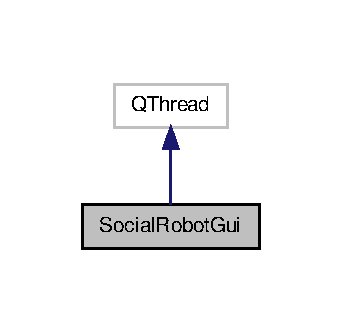
\includegraphics[width=277pt]{classSocialRobotGui__coll__graph}
\end{center}
\end{figure}
\subsection*{Signals}
\begin{DoxyCompactItemize}
\item 
void \hyperlink{classSocialRobotGui_aba07bb0bb3b8fa3f317539e9d6698aee}{update\_\-image} (const Mat \&)
\end{DoxyCompactItemize}
\subsection*{Public Member Functions}
\begin{DoxyCompactItemize}
\item 
\hyperlink{classSocialRobotGui_a5eaed12731bfb6967d261ae8433d2110}{SocialRobotGui} (int argc, char $\ast$$\ast$argv)
\item 
\hyperlink{classSocialRobotGui_afd21dde21c5d13e302cec9edda1e9abc}{$\sim$SocialRobotGui} ()
\item 
void \hyperlink{classSocialRobotGui_a3a979f567341925976347b3c1b735347}{init} ()
\item 
void \hyperlink{classSocialRobotGui_ac9171915901ff625cfbc1492ee8f267e}{run} ()
\item 
void \hyperlink{classSocialRobotGui_adeb531e38774a69cf8411aa18d2af8e2}{rgb\_\-cb} (const sensor\_\-msgs::ImageConstPtr \&msg)
\item 
void \hyperlink{classSocialRobotGui_a20bf403e17980a1c2d9f3efaf99a0ddd}{depth\_\-cb} (const sensor\_\-msgs::ImageConstPtr \&msg)
\item 
void \hyperlink{classSocialRobotGui_aac3a124449c975e2bc69fbc71d891e16}{rgb\_\-rois\_\-cb} (const \hyperlink{structsocial__robot_1_1RegionOfInterests__}{social\_\-robot::RegionOfInterests} \&msg)
\item 
void \hyperlink{classSocialRobotGui_a0c36cf4cb20fec7ec4d79abeb04b140d}{depth\_\-rois\_\-cb} (const \hyperlink{structsocial__robot_1_1RegionOfInterests__}{social\_\-robot::RegionOfInterests} \&msg)
\item 
void \hyperlink{classSocialRobotGui_a3333bd4377889eb97216ebfbb10f8104}{track\_\-rois\_\-cb} (const \hyperlink{structsocial__robot_1_1RegionOfInterests__}{social\_\-robot::RegionOfInterests} \&msg)
\item 
void \hyperlink{classSocialRobotGui_a77d605da08f98863b272ccef00b42666}{threshold\_\-template\_\-matching\_\-3d} (double threshold)
\item 
void \hyperlink{classSocialRobotGui_a5f6fedb5046ca5cc46c021cca4778385}{threshold\_\-scales} (int threshold)
\item 
void \hyperlink{classSocialRobotGui_a35d2e5e74b8e201cb269e8dd3c1b8dab}{threshold\_\-chamfer} (double threshold)
\item 
void \hyperlink{classSocialRobotGui_acdabf6f9c428cca8e0c0b74bd9035b82}{threshold\_\-arc\_\-low} (int threshold)
\item 
void \hyperlink{classSocialRobotGui_a5108ee2ec82ffc7561421e5c8576cef4}{threshold\_\-arc\_\-high} (int threshold)
\item 
void \hyperlink{classSocialRobotGui_a2345763f68b3da1cff958a9a24218da6}{threshold\_\-confidence} (double threshold)
\item 
void \hyperlink{classSocialRobotGui_a9931a08dd5eda16aa454d6edccdfb015}{threshold\_\-detection} (double threshold)
\item 
void \hyperlink{classSocialRobotGui_ac701acad18c8d5d0358886765ba8abb9}{threshold\_\-eucdis} (double threshold)
\end{DoxyCompactItemize}
\subsection*{Data Fields}
\begin{DoxyCompactItemize}
\item 
bool \hyperlink{classSocialRobotGui_a57c8e1f9be7edfe29703853268aa8aba}{display\_\-rgb\_\-faces}
\item 
bool \hyperlink{classSocialRobotGui_a1d32e49a34a1a0eafe6a7e160307bf82}{display\_\-depth\_\-faces}
\item 
bool \hyperlink{classSocialRobotGui_a28e6dc7627b92c85adb014bcaeb641bd}{display\_\-track\_\-faces}
\item 
bool \hyperlink{classSocialRobotGui_a29d1ccc0fd91a27bdd56364aef82d351}{display\_\-rgb\_\-image}
\item 
bool \hyperlink{classSocialRobotGui_aec418c0fe6ac3e995e2fedda35d0237e}{display\_\-depth\_\-image}
\end{DoxyCompactItemize}


\subsection{Constructor \& Destructor Documentation}
\hypertarget{classSocialRobotGui_a5eaed12731bfb6967d261ae8433d2110}{
\index{SocialRobotGui@{SocialRobotGui}!SocialRobotGui@{SocialRobotGui}}
\index{SocialRobotGui@{SocialRobotGui}!SocialRobotGui@{SocialRobotGui}}
\subsubsection[{SocialRobotGui}]{\setlength{\rightskip}{0pt plus 5cm}SocialRobotGui::SocialRobotGui (int {\em argc}, \/  char $\ast$$\ast$ {\em argv})}}
\label{classSocialRobotGui_a5eaed12731bfb6967d261ae8433d2110}
\hypertarget{classSocialRobotGui_afd21dde21c5d13e302cec9edda1e9abc}{
\index{SocialRobotGui@{SocialRobotGui}!$\sim$SocialRobotGui@{$\sim$SocialRobotGui}}
\index{$\sim$SocialRobotGui@{$\sim$SocialRobotGui}!SocialRobotGui@{SocialRobotGui}}
\subsubsection[{$\sim$SocialRobotGui}]{\setlength{\rightskip}{0pt plus 5cm}SocialRobotGui::$\sim$SocialRobotGui ()}}
\label{classSocialRobotGui_afd21dde21c5d13e302cec9edda1e9abc}


\subsection{Member Function Documentation}
\hypertarget{classSocialRobotGui_a20bf403e17980a1c2d9f3efaf99a0ddd}{
\index{SocialRobotGui@{SocialRobotGui}!depth\_\-cb@{depth\_\-cb}}
\index{depth\_\-cb@{depth\_\-cb}!SocialRobotGui@{SocialRobotGui}}
\subsubsection[{depth\_\-cb}]{\setlength{\rightskip}{0pt plus 5cm}void SocialRobotGui::depth\_\-cb (const sensor\_\-msgs::ImageConstPtr \& {\em msg})}}
\label{classSocialRobotGui_a20bf403e17980a1c2d9f3efaf99a0ddd}
\hypertarget{classSocialRobotGui_a0c36cf4cb20fec7ec4d79abeb04b140d}{
\index{SocialRobotGui@{SocialRobotGui}!depth\_\-rois\_\-cb@{depth\_\-rois\_\-cb}}
\index{depth\_\-rois\_\-cb@{depth\_\-rois\_\-cb}!SocialRobotGui@{SocialRobotGui}}
\subsubsection[{depth\_\-rois\_\-cb}]{\setlength{\rightskip}{0pt plus 5cm}void SocialRobotGui::depth\_\-rois\_\-cb (const {\bf social\_\-robot::RegionOfInterests} \& {\em msg})}}
\label{classSocialRobotGui_a0c36cf4cb20fec7ec4d79abeb04b140d}
\hypertarget{classSocialRobotGui_a3a979f567341925976347b3c1b735347}{
\index{SocialRobotGui@{SocialRobotGui}!init@{init}}
\index{init@{init}!SocialRobotGui@{SocialRobotGui}}
\subsubsection[{init}]{\setlength{\rightskip}{0pt plus 5cm}void SocialRobotGui::init ()}}
\label{classSocialRobotGui_a3a979f567341925976347b3c1b735347}
\hypertarget{classSocialRobotGui_adeb531e38774a69cf8411aa18d2af8e2}{
\index{SocialRobotGui@{SocialRobotGui}!rgb\_\-cb@{rgb\_\-cb}}
\index{rgb\_\-cb@{rgb\_\-cb}!SocialRobotGui@{SocialRobotGui}}
\subsubsection[{rgb\_\-cb}]{\setlength{\rightskip}{0pt plus 5cm}void SocialRobotGui::rgb\_\-cb (const sensor\_\-msgs::ImageConstPtr \& {\em msg})}}
\label{classSocialRobotGui_adeb531e38774a69cf8411aa18d2af8e2}
\hypertarget{classSocialRobotGui_aac3a124449c975e2bc69fbc71d891e16}{
\index{SocialRobotGui@{SocialRobotGui}!rgb\_\-rois\_\-cb@{rgb\_\-rois\_\-cb}}
\index{rgb\_\-rois\_\-cb@{rgb\_\-rois\_\-cb}!SocialRobotGui@{SocialRobotGui}}
\subsubsection[{rgb\_\-rois\_\-cb}]{\setlength{\rightskip}{0pt plus 5cm}void SocialRobotGui::rgb\_\-rois\_\-cb (const {\bf social\_\-robot::RegionOfInterests} \& {\em msg})}}
\label{classSocialRobotGui_aac3a124449c975e2bc69fbc71d891e16}
\hypertarget{classSocialRobotGui_ac9171915901ff625cfbc1492ee8f267e}{
\index{SocialRobotGui@{SocialRobotGui}!run@{run}}
\index{run@{run}!SocialRobotGui@{SocialRobotGui}}
\subsubsection[{run}]{\setlength{\rightskip}{0pt plus 5cm}void SocialRobotGui::run ()}}
\label{classSocialRobotGui_ac9171915901ff625cfbc1492ee8f267e}
\hypertarget{classSocialRobotGui_a5108ee2ec82ffc7561421e5c8576cef4}{
\index{SocialRobotGui@{SocialRobotGui}!threshold\_\-arc\_\-high@{threshold\_\-arc\_\-high}}
\index{threshold\_\-arc\_\-high@{threshold\_\-arc\_\-high}!SocialRobotGui@{SocialRobotGui}}
\subsubsection[{threshold\_\-arc\_\-high}]{\setlength{\rightskip}{0pt plus 5cm}void SocialRobotGui::threshold\_\-arc\_\-high (int {\em threshold})}}
\label{classSocialRobotGui_a5108ee2ec82ffc7561421e5c8576cef4}
\hypertarget{classSocialRobotGui_acdabf6f9c428cca8e0c0b74bd9035b82}{
\index{SocialRobotGui@{SocialRobotGui}!threshold\_\-arc\_\-low@{threshold\_\-arc\_\-low}}
\index{threshold\_\-arc\_\-low@{threshold\_\-arc\_\-low}!SocialRobotGui@{SocialRobotGui}}
\subsubsection[{threshold\_\-arc\_\-low}]{\setlength{\rightskip}{0pt plus 5cm}void SocialRobotGui::threshold\_\-arc\_\-low (int {\em threshold})}}
\label{classSocialRobotGui_acdabf6f9c428cca8e0c0b74bd9035b82}
\hypertarget{classSocialRobotGui_a35d2e5e74b8e201cb269e8dd3c1b8dab}{
\index{SocialRobotGui@{SocialRobotGui}!threshold\_\-chamfer@{threshold\_\-chamfer}}
\index{threshold\_\-chamfer@{threshold\_\-chamfer}!SocialRobotGui@{SocialRobotGui}}
\subsubsection[{threshold\_\-chamfer}]{\setlength{\rightskip}{0pt plus 5cm}void SocialRobotGui::threshold\_\-chamfer (double {\em threshold})}}
\label{classSocialRobotGui_a35d2e5e74b8e201cb269e8dd3c1b8dab}
\hypertarget{classSocialRobotGui_a2345763f68b3da1cff958a9a24218da6}{
\index{SocialRobotGui@{SocialRobotGui}!threshold\_\-confidence@{threshold\_\-confidence}}
\index{threshold\_\-confidence@{threshold\_\-confidence}!SocialRobotGui@{SocialRobotGui}}
\subsubsection[{threshold\_\-confidence}]{\setlength{\rightskip}{0pt plus 5cm}void SocialRobotGui::threshold\_\-confidence (double {\em threshold})}}
\label{classSocialRobotGui_a2345763f68b3da1cff958a9a24218da6}
\hypertarget{classSocialRobotGui_a9931a08dd5eda16aa454d6edccdfb015}{
\index{SocialRobotGui@{SocialRobotGui}!threshold\_\-detection@{threshold\_\-detection}}
\index{threshold\_\-detection@{threshold\_\-detection}!SocialRobotGui@{SocialRobotGui}}
\subsubsection[{threshold\_\-detection}]{\setlength{\rightskip}{0pt plus 5cm}void SocialRobotGui::threshold\_\-detection (double {\em threshold})}}
\label{classSocialRobotGui_a9931a08dd5eda16aa454d6edccdfb015}
\hypertarget{classSocialRobotGui_ac701acad18c8d5d0358886765ba8abb9}{
\index{SocialRobotGui@{SocialRobotGui}!threshold\_\-eucdis@{threshold\_\-eucdis}}
\index{threshold\_\-eucdis@{threshold\_\-eucdis}!SocialRobotGui@{SocialRobotGui}}
\subsubsection[{threshold\_\-eucdis}]{\setlength{\rightskip}{0pt plus 5cm}void SocialRobotGui::threshold\_\-eucdis (double {\em threshold})}}
\label{classSocialRobotGui_ac701acad18c8d5d0358886765ba8abb9}
\hypertarget{classSocialRobotGui_a5f6fedb5046ca5cc46c021cca4778385}{
\index{SocialRobotGui@{SocialRobotGui}!threshold\_\-scales@{threshold\_\-scales}}
\index{threshold\_\-scales@{threshold\_\-scales}!SocialRobotGui@{SocialRobotGui}}
\subsubsection[{threshold\_\-scales}]{\setlength{\rightskip}{0pt plus 5cm}void SocialRobotGui::threshold\_\-scales (int {\em threshold})}}
\label{classSocialRobotGui_a5f6fedb5046ca5cc46c021cca4778385}
\hypertarget{classSocialRobotGui_a77d605da08f98863b272ccef00b42666}{
\index{SocialRobotGui@{SocialRobotGui}!threshold\_\-template\_\-matching\_\-3d@{threshold\_\-template\_\-matching\_\-3d}}
\index{threshold\_\-template\_\-matching\_\-3d@{threshold\_\-template\_\-matching\_\-3d}!SocialRobotGui@{SocialRobotGui}}
\subsubsection[{threshold\_\-template\_\-matching\_\-3d}]{\setlength{\rightskip}{0pt plus 5cm}void SocialRobotGui::threshold\_\-template\_\-matching\_\-3d (double {\em threshold})}}
\label{classSocialRobotGui_a77d605da08f98863b272ccef00b42666}
\hypertarget{classSocialRobotGui_a3333bd4377889eb97216ebfbb10f8104}{
\index{SocialRobotGui@{SocialRobotGui}!track\_\-rois\_\-cb@{track\_\-rois\_\-cb}}
\index{track\_\-rois\_\-cb@{track\_\-rois\_\-cb}!SocialRobotGui@{SocialRobotGui}}
\subsubsection[{track\_\-rois\_\-cb}]{\setlength{\rightskip}{0pt plus 5cm}void SocialRobotGui::track\_\-rois\_\-cb (const {\bf social\_\-robot::RegionOfInterests} \& {\em msg})}}
\label{classSocialRobotGui_a3333bd4377889eb97216ebfbb10f8104}
\hypertarget{classSocialRobotGui_aba07bb0bb3b8fa3f317539e9d6698aee}{
\index{SocialRobotGui@{SocialRobotGui}!update\_\-image@{update\_\-image}}
\index{update\_\-image@{update\_\-image}!SocialRobotGui@{SocialRobotGui}}
\subsubsection[{update\_\-image}]{\setlength{\rightskip}{0pt plus 5cm}void SocialRobotGui::update\_\-image (const Mat \& {\em \_\-t1})\hspace{0.3cm}{\ttfamily  \mbox{[}signal\mbox{]}}}}
\label{classSocialRobotGui_aba07bb0bb3b8fa3f317539e9d6698aee}


\subsection{Field Documentation}
\hypertarget{classSocialRobotGui_a1d32e49a34a1a0eafe6a7e160307bf82}{
\index{SocialRobotGui@{SocialRobotGui}!display\_\-depth\_\-faces@{display\_\-depth\_\-faces}}
\index{display\_\-depth\_\-faces@{display\_\-depth\_\-faces}!SocialRobotGui@{SocialRobotGui}}
\subsubsection[{display\_\-depth\_\-faces}]{\setlength{\rightskip}{0pt plus 5cm}bool {\bf SocialRobotGui::display\_\-depth\_\-faces}}}
\label{classSocialRobotGui_a1d32e49a34a1a0eafe6a7e160307bf82}
\hypertarget{classSocialRobotGui_aec418c0fe6ac3e995e2fedda35d0237e}{
\index{SocialRobotGui@{SocialRobotGui}!display\_\-depth\_\-image@{display\_\-depth\_\-image}}
\index{display\_\-depth\_\-image@{display\_\-depth\_\-image}!SocialRobotGui@{SocialRobotGui}}
\subsubsection[{display\_\-depth\_\-image}]{\setlength{\rightskip}{0pt plus 5cm}bool {\bf SocialRobotGui::display\_\-depth\_\-image}}}
\label{classSocialRobotGui_aec418c0fe6ac3e995e2fedda35d0237e}
\hypertarget{classSocialRobotGui_a57c8e1f9be7edfe29703853268aa8aba}{
\index{SocialRobotGui@{SocialRobotGui}!display\_\-rgb\_\-faces@{display\_\-rgb\_\-faces}}
\index{display\_\-rgb\_\-faces@{display\_\-rgb\_\-faces}!SocialRobotGui@{SocialRobotGui}}
\subsubsection[{display\_\-rgb\_\-faces}]{\setlength{\rightskip}{0pt plus 5cm}bool {\bf SocialRobotGui::display\_\-rgb\_\-faces}}}
\label{classSocialRobotGui_a57c8e1f9be7edfe29703853268aa8aba}
\hypertarget{classSocialRobotGui_a29d1ccc0fd91a27bdd56364aef82d351}{
\index{SocialRobotGui@{SocialRobotGui}!display\_\-rgb\_\-image@{display\_\-rgb\_\-image}}
\index{display\_\-rgb\_\-image@{display\_\-rgb\_\-image}!SocialRobotGui@{SocialRobotGui}}
\subsubsection[{display\_\-rgb\_\-image}]{\setlength{\rightskip}{0pt plus 5cm}bool {\bf SocialRobotGui::display\_\-rgb\_\-image}}}
\label{classSocialRobotGui_a29d1ccc0fd91a27bdd56364aef82d351}
\hypertarget{classSocialRobotGui_a28e6dc7627b92c85adb014bcaeb641bd}{
\index{SocialRobotGui@{SocialRobotGui}!display\_\-track\_\-faces@{display\_\-track\_\-faces}}
\index{display\_\-track\_\-faces@{display\_\-track\_\-faces}!SocialRobotGui@{SocialRobotGui}}
\subsubsection[{display\_\-track\_\-faces}]{\setlength{\rightskip}{0pt plus 5cm}bool {\bf SocialRobotGui::display\_\-track\_\-faces}}}
\label{classSocialRobotGui_a28e6dc7627b92c85adb014bcaeb641bd}


The documentation for this class was generated from the following files:\begin{DoxyCompactItemize}
\item 
\hyperlink{SocialRobotGui_8h}{SocialRobotGui.h}\item 
\hyperlink{moc__SocialRobotGui_8cxx}{moc\_\-SocialRobotGui.cxx}\item 
\hyperlink{SocialRobotGui_8cpp}{SocialRobotGui.cpp}\end{DoxyCompactItemize}

\hypertarget{classStateData}{
\section{StateData Class Reference}
\label{classStateData}\index{StateData@{StateData}}
}


{\ttfamily \#include $<$StateData.h$>$}



Collaboration diagram for StateData:\nopagebreak
\begin{figure}[H]
\begin{center}
\leavevmode
\includegraphics[height=400pt]{classStateData__coll__graph}
\end{center}
\end{figure}
\subsection*{Public Member Functions}
\begin{DoxyCompactItemize}
\item 
\hyperlink{classStateData_a3bbfa4301403ebf5d24d5d16cf246b88}{StateData} (void)
\item 
void \hyperlink{classStateData_af4bbe24b619137cba16b7b85970e1bd7}{tracking} (double cost=0.01)
\item 
void \hyperlink{classStateData_a3fe497a97247af50f8eb876d6284da69}{initialise} (int \hyperlink{social__robot_8cpp_acf574bc864f7f0fc111320f1d6c449d5}{num\_\-particles}, Mat image\_\-, Rect selection\_\-, Mat image\_\-depth\_\-, int hist\_\-type\_\-)
\item 
Rect \hyperlink{classStateData_aa2c20a09eecd353d4454e707ac17f143}{get\_\-target\_\-position} (void)
\item 
void \hyperlink{classStateData_a2b26ea86bd2d1d3d37debec000fefa01}{update\_\-target\_\-histogram} (Mat \&newimage, Mat \&newdepth, Rect new\_\-selection)
\end{DoxyCompactItemize}
\subsection*{Data Fields}
\begin{DoxyCompactItemize}
\item 
Mat \hyperlink{classStateData_ab1a1e2be2b9a55c78bc579024d30cf64}{image}
\item 
Mat \hyperlink{classStateData_a662c82a423f855845f2be8700af72817}{image\_\-depth}
\item 
Mat \hyperlink{classStateData_ac778c44e62237a225361a80894a48ee8}{target}
\item 
Mat \hyperlink{classStateData_af93e02e6025c07b7a383b2e755f52dca}{target\_\-histogram}
\item 
Rect \hyperlink{classStateData_afea0bc5d1743e2db008238bfe9f574ce}{selection}
\item 
double \hyperlink{classStateData_abe87d63070a9fc98cd9f1475495725e6}{detection\_\-confidence}
\item 
int \hyperlink{classStateData_a14b4b6d403b4517d7102f49a501d51ed}{hist\_\-type}
\item 
bool \hyperlink{classStateData_ad5f3d2a522bfdcff47e7d028bf19f012}{is\_\-associated}
\item 
\hyperlink{classParticleFilter}{ParticleFilter} $\ast$ \hyperlink{classStateData_a42c35fd351a6634b67fd1fd2f5a09cf4}{filter}
\end{DoxyCompactItemize}


\subsection{Constructor \& Destructor Documentation}
\hypertarget{classStateData_a3bbfa4301403ebf5d24d5d16cf246b88}{
\index{StateData@{StateData}!StateData@{StateData}}
\index{StateData@{StateData}!StateData@{StateData}}
\subsubsection[{StateData}]{\setlength{\rightskip}{0pt plus 5cm}StateData::StateData (void)}}
\label{classStateData_a3bbfa4301403ebf5d24d5d16cf246b88}


\subsection{Member Function Documentation}
\hypertarget{classStateData_aa2c20a09eecd353d4454e707ac17f143}{
\index{StateData@{StateData}!get\_\-target\_\-position@{get\_\-target\_\-position}}
\index{get\_\-target\_\-position@{get\_\-target\_\-position}!StateData@{StateData}}
\subsubsection[{get\_\-target\_\-position}]{\setlength{\rightskip}{0pt plus 5cm}Rect StateData::get\_\-target\_\-position (void)}}
\label{classStateData_aa2c20a09eecd353d4454e707ac17f143}
\hypertarget{classStateData_a3fe497a97247af50f8eb876d6284da69}{
\index{StateData@{StateData}!initialise@{initialise}}
\index{initialise@{initialise}!StateData@{StateData}}
\subsubsection[{initialise}]{\setlength{\rightskip}{0pt plus 5cm}void StateData::initialise (int {\em num\_\-particles}, \/  Mat {\em image\_\-}, \/  Rect {\em selection\_\-}, \/  Mat {\em image\_\-depth\_\-}, \/  int {\em hist\_\-type\_\-})}}
\label{classStateData_a3fe497a97247af50f8eb876d6284da69}
\hypertarget{classStateData_af4bbe24b619137cba16b7b85970e1bd7}{
\index{StateData@{StateData}!tracking@{tracking}}
\index{tracking@{tracking}!StateData@{StateData}}
\subsubsection[{tracking}]{\setlength{\rightskip}{0pt plus 5cm}void StateData::tracking (double {\em cost} = {\ttfamily 0.01})}}
\label{classStateData_af4bbe24b619137cba16b7b85970e1bd7}
\hypertarget{classStateData_a2b26ea86bd2d1d3d37debec000fefa01}{
\index{StateData@{StateData}!update\_\-target\_\-histogram@{update\_\-target\_\-histogram}}
\index{update\_\-target\_\-histogram@{update\_\-target\_\-histogram}!StateData@{StateData}}
\subsubsection[{update\_\-target\_\-histogram}]{\setlength{\rightskip}{0pt plus 5cm}void StateData::update\_\-target\_\-histogram (Mat \& {\em newimage}, \/  Mat \& {\em newdepth}, \/  Rect {\em new\_\-selection})}}
\label{classStateData_a2b26ea86bd2d1d3d37debec000fefa01}


\subsection{Field Documentation}
\hypertarget{classStateData_abe87d63070a9fc98cd9f1475495725e6}{
\index{StateData@{StateData}!detection\_\-confidence@{detection\_\-confidence}}
\index{detection\_\-confidence@{detection\_\-confidence}!StateData@{StateData}}
\subsubsection[{detection\_\-confidence}]{\setlength{\rightskip}{0pt plus 5cm}double {\bf StateData::detection\_\-confidence}}}
\label{classStateData_abe87d63070a9fc98cd9f1475495725e6}
\hypertarget{classStateData_a42c35fd351a6634b67fd1fd2f5a09cf4}{
\index{StateData@{StateData}!filter@{filter}}
\index{filter@{filter}!StateData@{StateData}}
\subsubsection[{filter}]{\setlength{\rightskip}{0pt plus 5cm}{\bf ParticleFilter}$\ast$ {\bf StateData::filter}}}
\label{classStateData_a42c35fd351a6634b67fd1fd2f5a09cf4}
\hypertarget{classStateData_a14b4b6d403b4517d7102f49a501d51ed}{
\index{StateData@{StateData}!hist\_\-type@{hist\_\-type}}
\index{hist\_\-type@{hist\_\-type}!StateData@{StateData}}
\subsubsection[{hist\_\-type}]{\setlength{\rightskip}{0pt plus 5cm}int {\bf StateData::hist\_\-type}}}
\label{classStateData_a14b4b6d403b4517d7102f49a501d51ed}
\hypertarget{classStateData_ab1a1e2be2b9a55c78bc579024d30cf64}{
\index{StateData@{StateData}!image@{image}}
\index{image@{image}!StateData@{StateData}}
\subsubsection[{image}]{\setlength{\rightskip}{0pt plus 5cm}Mat {\bf StateData::image}}}
\label{classStateData_ab1a1e2be2b9a55c78bc579024d30cf64}
\hypertarget{classStateData_a662c82a423f855845f2be8700af72817}{
\index{StateData@{StateData}!image\_\-depth@{image\_\-depth}}
\index{image\_\-depth@{image\_\-depth}!StateData@{StateData}}
\subsubsection[{image\_\-depth}]{\setlength{\rightskip}{0pt plus 5cm}Mat {\bf StateData::image\_\-depth}}}
\label{classStateData_a662c82a423f855845f2be8700af72817}
\hypertarget{classStateData_ad5f3d2a522bfdcff47e7d028bf19f012}{
\index{StateData@{StateData}!is\_\-associated@{is\_\-associated}}
\index{is\_\-associated@{is\_\-associated}!StateData@{StateData}}
\subsubsection[{is\_\-associated}]{\setlength{\rightskip}{0pt plus 5cm}bool {\bf StateData::is\_\-associated}}}
\label{classStateData_ad5f3d2a522bfdcff47e7d028bf19f012}
\hypertarget{classStateData_afea0bc5d1743e2db008238bfe9f574ce}{
\index{StateData@{StateData}!selection@{selection}}
\index{selection@{selection}!StateData@{StateData}}
\subsubsection[{selection}]{\setlength{\rightskip}{0pt plus 5cm}Rect {\bf StateData::selection}}}
\label{classStateData_afea0bc5d1743e2db008238bfe9f574ce}
\hypertarget{classStateData_ac778c44e62237a225361a80894a48ee8}{
\index{StateData@{StateData}!target@{target}}
\index{target@{target}!StateData@{StateData}}
\subsubsection[{target}]{\setlength{\rightskip}{0pt plus 5cm}Mat {\bf StateData::target}}}
\label{classStateData_ac778c44e62237a225361a80894a48ee8}
\hypertarget{classStateData_af93e02e6025c07b7a383b2e755f52dca}{
\index{StateData@{StateData}!target\_\-histogram@{target\_\-histogram}}
\index{target\_\-histogram@{target\_\-histogram}!StateData@{StateData}}
\subsubsection[{target\_\-histogram}]{\setlength{\rightskip}{0pt plus 5cm}Mat {\bf StateData::target\_\-histogram}}}
\label{classStateData_af93e02e6025c07b7a383b2e755f52dca}


The documentation for this class was generated from the following files:\begin{DoxyCompactItemize}
\item 
\hyperlink{StateData_8h}{StateData.h}\item 
\hyperlink{StateData_8cpp}{StateData.cpp}\end{DoxyCompactItemize}

\hypertarget{classTemplate}{
\section{Template Class Reference}
\label{classTemplate}\index{Template@{Template}}
}


This class contains the 2D and 3D templates for matching.  




{\ttfamily \#include $<$Template.h$>$}

\subsection*{Public Member Functions}
\begin{DoxyCompactItemize}
\item 
\hyperlink{classTemplate_afea5166b9ca0022fe21c2ed4882c161a}{Template} ()
\item 
\hyperlink{classTemplate_a9234aea5815f2a8d8bde56f635b2d2f3}{Template} (cv::Mat, cv::Mat)
\end{DoxyCompactItemize}
\subsection*{Data Fields}
\begin{DoxyCompactItemize}
\item 
cv::Mat \hyperlink{classTemplate_a65d3e446fb6ac165be19da2d747e85ed}{template2d}
\item 
cv::Mat \hyperlink{classTemplate_a27b16dc049359b1ac3ee24b08841ba56}{template3d}
\end{DoxyCompactItemize}


\subsection{Detailed Description}
This class contains the 2D and 3D templates for matching. \begin{DoxyAuthor}{Author}
Social Robot 
\end{DoxyAuthor}


\subsection{Constructor \& Destructor Documentation}
\hypertarget{classTemplate_afea5166b9ca0022fe21c2ed4882c161a}{
\index{Template@{Template}!Template@{Template}}
\index{Template@{Template}!Template@{Template}}
\subsubsection[{Template}]{\setlength{\rightskip}{0pt plus 5cm}Template::Template ()}}
\label{classTemplate_afea5166b9ca0022fe21c2ed4882c161a}
Default Constructor. \hypertarget{classTemplate_a9234aea5815f2a8d8bde56f635b2d2f3}{
\index{Template@{Template}!Template@{Template}}
\index{Template@{Template}!Template@{Template}}
\subsubsection[{Template}]{\setlength{\rightskip}{0pt plus 5cm}Template::Template (cv::Mat {\em template2d}, \/  cv::Mat {\em template3d})}}
\label{classTemplate_a9234aea5815f2a8d8bde56f635b2d2f3}
Constructor given 2D and 3D templates. 
\begin{DoxyParams}{Parameters}
\item[{\em template2d}]A Mat containing a binary image. \item[{\em template3d}]A Mat containing a grayscale image. Notice that template3d is a grayscale image, it is used 3d when the matching is done with the depth image. \end{DoxyParams}


\subsection{Field Documentation}
\hypertarget{classTemplate_a65d3e446fb6ac165be19da2d747e85ed}{
\index{Template@{Template}!template2d@{template2d}}
\index{template2d@{template2d}!Template@{Template}}
\subsubsection[{template2d}]{\setlength{\rightskip}{0pt plus 5cm}cv::Mat {\bf Template::template2d}}}
\label{classTemplate_a65d3e446fb6ac165be19da2d747e85ed}
\hypertarget{classTemplate_a27b16dc049359b1ac3ee24b08841ba56}{
\index{Template@{Template}!template3d@{template3d}}
\index{template3d@{template3d}!Template@{Template}}
\subsubsection[{template3d}]{\setlength{\rightskip}{0pt plus 5cm}cv::Mat {\bf Template::template3d}}}
\label{classTemplate_a27b16dc049359b1ac3ee24b08841ba56}


The documentation for this class was generated from the following files:\begin{DoxyCompactItemize}
\item 
\hyperlink{Template_8h}{Template.h}\item 
\hyperlink{Template_8cpp}{Template.cpp}\end{DoxyCompactItemize}

\hypertarget{classViewPort}{\section{View\-Port Class Reference}
\label{classViewPort}\index{View\-Port@{View\-Port}}
}


{\ttfamily \#include $<$window\-\_\-\-Q\-T.\-h$>$}



Inheritance diagram for View\-Port\-:\nopagebreak
\begin{figure}[H]
\begin{center}
\leavevmode
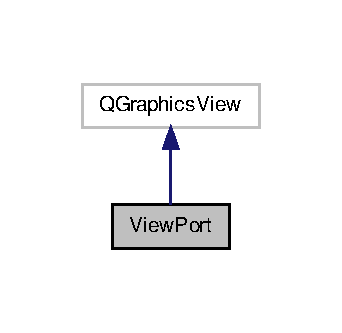
\includegraphics[width=164pt]{classViewPort__inherit__graph}
\end{center}
\end{figure}


Collaboration diagram for View\-Port\-:\nopagebreak
\begin{figure}[H]
\begin{center}
\leavevmode
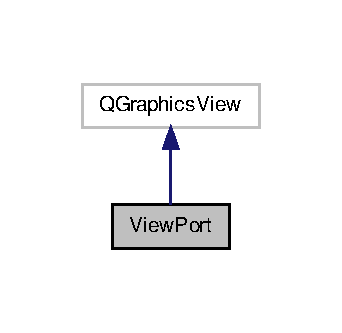
\includegraphics[width=164pt]{classViewPort__coll__graph}
\end{center}
\end{figure}
\subsection*{Public Slots}
\begin{DoxyCompactItemize}
\item 
void \hyperlink{classViewPort_af68a292bada1aadd5b3cbcd5cd86620c}{scale\-View} (qreal scale\-Factor, Q\-Point\-F center)
\item 
void \hyperlink{classViewPort_a60f919b3f7329bb5de060fa3befda08b}{img\-Region} ()
\item 
void \hyperlink{classViewPort_a3e318f428a0d0cc2e5c3835f1c77cc06}{move\-View} (Q\-Point\-F delta)
\item 
void \hyperlink{classViewPort_af9e56726827ee1679b536d90586b3add}{reset\-Zoom} ()
\item 
void \hyperlink{classViewPort_a4a67d1ac61dfdf063909b9fa5299893f}{Zoom\-In} ()
\item 
void \hyperlink{classViewPort_a4f26ce0e84539f49b95aa5d43820bb85}{Zoom\-Out} ()
\item 
void \hyperlink{classViewPort_ab8d8fbc8a150d158840e73dc3d28d4e9}{sift\-Window\-On\-Left} ()
\item 
void \hyperlink{classViewPort_ad75dd8cdf0fcefa9f3afb7af78ffa1fc}{sift\-Window\-On\-Right} ()
\item 
void \hyperlink{classViewPort_a539a1c2895777e89b1431146ccb26a26}{sift\-Window\-On\-Up} ()
\item 
void \hyperlink{classViewPort_aa05e98b5c021662068856f9b8f25a299}{sift\-Window\-On\-Down} ()
\item 
void \hyperlink{classViewPort_a7a1fec5745e2bd12c11f0f4a8c17183f}{resize\-Event} (Q\-Resize\-Event $\ast$)
\item 
void \hyperlink{classViewPort_a69445bb6b5b203923b6707b583cdc0d8}{save\-View} ()
\item 
void \hyperlink{classViewPort_af3c98b34c5ff602bd74c5b95425de4a9}{context\-Menu\-Event} (Q\-Context\-Menu\-Event $\ast$event)
\end{DoxyCompactItemize}
\subsection*{Public Member Functions}
\begin{DoxyCompactItemize}
\item 
\hyperlink{classViewPort_ae986eca6567919eccfa84fa11d152519}{View\-Port} (\hyperlink{classCvWindow}{Cv\-Window} $\ast$central\-Widget, int mode=\hyperlink{window__QT_8h_adf764cbdea00d65edcd07bb9953ad2b7a8f4516cd4423037ff9e7c533c4084e64}{C\-V\-\_\-\-M\-O\-D\-E\-\_\-\-N\-O\-R\-M\-A\-L}, int keep\-Ratio=C\-V\-\_\-\-W\-I\-N\-D\-O\-W\-\_\-\-K\-E\-E\-P\-R\-A\-T\-I\-O)
\item 
\hyperlink{classViewPort_aa9e30578206a4c74b8e3e0bf1cbed5a1}{$\sim$\-View\-Port} ()
\item 
void \hyperlink{classViewPort_a19c83263889430a83e5f9d1aaee4741b}{update\-Image} (const Cv\-Arr $\ast$arr)
\item 
void \hyperlink{classViewPort_a2618b2c40f1770ab153cbae4da9c5313}{start\-Display\-Info} (Q\-String text, int delayms)
\item 
void \hyperlink{classViewPort_a725688baa203c6247e9a147acaa7597a}{set\-Mouse\-Call\-Back} (Cv\-Mouse\-Callback m, void $\ast$param)
\item 
int \hyperlink{classViewPort_a969eb1a036822f1f500dd832c1f45d11}{get\-Ratio} ()
\item 
void \hyperlink{classViewPort_ad250b6cf4dd6d571128a7ad0d4d98175}{set\-Ratio} (int arg)
\end{DoxyCompactItemize}
\subsection*{Data Fields}
\begin{DoxyCompactItemize}
\item 
Q\-Transform \hyperlink{classViewPort_a4404db6e34a91d2e2e4c5026840a2adc}{param\-\_\-matrix\-World}
\item 
int \hyperlink{classViewPort_a2ad627e7c8f030da5b252cfbb056164b}{param\-\_\-keep\-Ratio}
\item 
Cv\-Mat $\ast$ \hyperlink{classViewPort_af6a3576406241b379379cc6d1a6d0c4f}{image2\-Draw\-\_\-mat}
\item 
Q\-Image \hyperlink{classViewPort_affb4d66105d8c57b62a8d1ca3a2f2aae}{image2\-Draw\-\_\-qt}
\item 
Q\-Image \hyperlink{classViewPort_a69c446903d67c1e328c8398341c2da21}{image2\-Draw\-\_\-qt\-\_\-resized}
\item 
int \hyperlink{classViewPort_abdd3f74adf3deb4bc1808f669d8815a4}{mode\-\_\-display}
\item 
int \hyperlink{classViewPort_a023381fa2838df1c3ef3a9183f4abbd1}{nb\-Channel\-Origin\-Image}
\end{DoxyCompactItemize}


\subsection{Constructor \& Destructor Documentation}
\hypertarget{classViewPort_ae986eca6567919eccfa84fa11d152519}{\index{View\-Port@{View\-Port}!View\-Port@{View\-Port}}
\index{View\-Port@{View\-Port}!ViewPort@{View\-Port}}
\subsubsection[{View\-Port}]{\setlength{\rightskip}{0pt plus 5cm}View\-Port\-::\-View\-Port (
\begin{DoxyParamCaption}
\item[{{\bf Cv\-Window} $\ast$}]{central\-Widget, }
\item[{int}]{mode = {\ttfamily {\bf C\-V\-\_\-\-M\-O\-D\-E\-\_\-\-N\-O\-R\-M\-A\-L}}, }
\item[{int}]{keep\-Ratio = {\ttfamily CV\-\_\-WINDOW\-\_\-KEEPRATIO}}
\end{DoxyParamCaption}
)}}\label{classViewPort_ae986eca6567919eccfa84fa11d152519}
\hypertarget{classViewPort_aa9e30578206a4c74b8e3e0bf1cbed5a1}{\index{View\-Port@{View\-Port}!$\sim$\-View\-Port@{$\sim$\-View\-Port}}
\index{$\sim$\-View\-Port@{$\sim$\-View\-Port}!ViewPort@{View\-Port}}
\subsubsection[{$\sim$\-View\-Port}]{\setlength{\rightskip}{0pt plus 5cm}View\-Port\-::$\sim$\-View\-Port (
\begin{DoxyParamCaption}
{}
\end{DoxyParamCaption}
)}}\label{classViewPort_aa9e30578206a4c74b8e3e0bf1cbed5a1}


\subsection{Member Function Documentation}
\hypertarget{classViewPort_af3c98b34c5ff602bd74c5b95425de4a9}{\index{View\-Port@{View\-Port}!context\-Menu\-Event@{context\-Menu\-Event}}
\index{context\-Menu\-Event@{context\-Menu\-Event}!ViewPort@{View\-Port}}
\subsubsection[{context\-Menu\-Event}]{\setlength{\rightskip}{0pt plus 5cm}void View\-Port\-::context\-Menu\-Event (
\begin{DoxyParamCaption}
\item[{Q\-Context\-Menu\-Event $\ast$}]{event}
\end{DoxyParamCaption}
)\hspace{0.3cm}{\ttfamily [slot]}}}\label{classViewPort_af3c98b34c5ff602bd74c5b95425de4a9}
\hypertarget{classViewPort_a969eb1a036822f1f500dd832c1f45d11}{\index{View\-Port@{View\-Port}!get\-Ratio@{get\-Ratio}}
\index{get\-Ratio@{get\-Ratio}!ViewPort@{View\-Port}}
\subsubsection[{get\-Ratio}]{\setlength{\rightskip}{0pt plus 5cm}int View\-Port\-::get\-Ratio (
\begin{DoxyParamCaption}
{}
\end{DoxyParamCaption}
)}}\label{classViewPort_a969eb1a036822f1f500dd832c1f45d11}
\hypertarget{classViewPort_a60f919b3f7329bb5de060fa3befda08b}{\index{View\-Port@{View\-Port}!img\-Region@{img\-Region}}
\index{img\-Region@{img\-Region}!ViewPort@{View\-Port}}
\subsubsection[{img\-Region}]{\setlength{\rightskip}{0pt plus 5cm}void View\-Port\-::img\-Region (
\begin{DoxyParamCaption}
{}
\end{DoxyParamCaption}
)\hspace{0.3cm}{\ttfamily [slot]}}}\label{classViewPort_a60f919b3f7329bb5de060fa3befda08b}
\hypertarget{classViewPort_a3e318f428a0d0cc2e5c3835f1c77cc06}{\index{View\-Port@{View\-Port}!move\-View@{move\-View}}
\index{move\-View@{move\-View}!ViewPort@{View\-Port}}
\subsubsection[{move\-View}]{\setlength{\rightskip}{0pt plus 5cm}void View\-Port\-::move\-View (
\begin{DoxyParamCaption}
\item[{Q\-Point\-F}]{delta}
\end{DoxyParamCaption}
)\hspace{0.3cm}{\ttfamily [slot]}}}\label{classViewPort_a3e318f428a0d0cc2e5c3835f1c77cc06}
\hypertarget{classViewPort_af9e56726827ee1679b536d90586b3add}{\index{View\-Port@{View\-Port}!reset\-Zoom@{reset\-Zoom}}
\index{reset\-Zoom@{reset\-Zoom}!ViewPort@{View\-Port}}
\subsubsection[{reset\-Zoom}]{\setlength{\rightskip}{0pt plus 5cm}void View\-Port\-::reset\-Zoom (
\begin{DoxyParamCaption}
{}
\end{DoxyParamCaption}
)\hspace{0.3cm}{\ttfamily [slot]}}}\label{classViewPort_af9e56726827ee1679b536d90586b3add}
\hypertarget{classViewPort_a7a1fec5745e2bd12c11f0f4a8c17183f}{\index{View\-Port@{View\-Port}!resize\-Event@{resize\-Event}}
\index{resize\-Event@{resize\-Event}!ViewPort@{View\-Port}}
\subsubsection[{resize\-Event}]{\setlength{\rightskip}{0pt plus 5cm}void View\-Port\-::resize\-Event (
\begin{DoxyParamCaption}
\item[{Q\-Resize\-Event $\ast$}]{event}
\end{DoxyParamCaption}
)\hspace{0.3cm}{\ttfamily [slot]}}}\label{classViewPort_a7a1fec5745e2bd12c11f0f4a8c17183f}
\hypertarget{classViewPort_a69445bb6b5b203923b6707b583cdc0d8}{\index{View\-Port@{View\-Port}!save\-View@{save\-View}}
\index{save\-View@{save\-View}!ViewPort@{View\-Port}}
\subsubsection[{save\-View}]{\setlength{\rightskip}{0pt plus 5cm}void View\-Port\-::save\-View (
\begin{DoxyParamCaption}
{}
\end{DoxyParamCaption}
)\hspace{0.3cm}{\ttfamily [slot]}}}\label{classViewPort_a69445bb6b5b203923b6707b583cdc0d8}
\hypertarget{classViewPort_af68a292bada1aadd5b3cbcd5cd86620c}{\index{View\-Port@{View\-Port}!scale\-View@{scale\-View}}
\index{scale\-View@{scale\-View}!ViewPort@{View\-Port}}
\subsubsection[{scale\-View}]{\setlength{\rightskip}{0pt plus 5cm}void View\-Port\-::scale\-View (
\begin{DoxyParamCaption}
\item[{qreal}]{scale\-Factor, }
\item[{Q\-Point\-F}]{center}
\end{DoxyParamCaption}
)\hspace{0.3cm}{\ttfamily [slot]}}}\label{classViewPort_af68a292bada1aadd5b3cbcd5cd86620c}
\hypertarget{classViewPort_a725688baa203c6247e9a147acaa7597a}{\index{View\-Port@{View\-Port}!set\-Mouse\-Call\-Back@{set\-Mouse\-Call\-Back}}
\index{set\-Mouse\-Call\-Back@{set\-Mouse\-Call\-Back}!ViewPort@{View\-Port}}
\subsubsection[{set\-Mouse\-Call\-Back}]{\setlength{\rightskip}{0pt plus 5cm}void View\-Port\-::set\-Mouse\-Call\-Back (
\begin{DoxyParamCaption}
\item[{Cv\-Mouse\-Callback}]{m, }
\item[{void $\ast$}]{param}
\end{DoxyParamCaption}
)}}\label{classViewPort_a725688baa203c6247e9a147acaa7597a}
\hypertarget{classViewPort_ad250b6cf4dd6d571128a7ad0d4d98175}{\index{View\-Port@{View\-Port}!set\-Ratio@{set\-Ratio}}
\index{set\-Ratio@{set\-Ratio}!ViewPort@{View\-Port}}
\subsubsection[{set\-Ratio}]{\setlength{\rightskip}{0pt plus 5cm}void View\-Port\-::set\-Ratio (
\begin{DoxyParamCaption}
\item[{int}]{arg}
\end{DoxyParamCaption}
)}}\label{classViewPort_ad250b6cf4dd6d571128a7ad0d4d98175}
\hypertarget{classViewPort_aa05e98b5c021662068856f9b8f25a299}{\index{View\-Port@{View\-Port}!sift\-Window\-On\-Down@{sift\-Window\-On\-Down}}
\index{sift\-Window\-On\-Down@{sift\-Window\-On\-Down}!ViewPort@{View\-Port}}
\subsubsection[{sift\-Window\-On\-Down}]{\setlength{\rightskip}{0pt plus 5cm}void View\-Port\-::sift\-Window\-On\-Down (
\begin{DoxyParamCaption}
{}
\end{DoxyParamCaption}
)\hspace{0.3cm}{\ttfamily [slot]}}}\label{classViewPort_aa05e98b5c021662068856f9b8f25a299}
\hypertarget{classViewPort_ab8d8fbc8a150d158840e73dc3d28d4e9}{\index{View\-Port@{View\-Port}!sift\-Window\-On\-Left@{sift\-Window\-On\-Left}}
\index{sift\-Window\-On\-Left@{sift\-Window\-On\-Left}!ViewPort@{View\-Port}}
\subsubsection[{sift\-Window\-On\-Left}]{\setlength{\rightskip}{0pt plus 5cm}void View\-Port\-::sift\-Window\-On\-Left (
\begin{DoxyParamCaption}
{}
\end{DoxyParamCaption}
)\hspace{0.3cm}{\ttfamily [slot]}}}\label{classViewPort_ab8d8fbc8a150d158840e73dc3d28d4e9}
\hypertarget{classViewPort_ad75dd8cdf0fcefa9f3afb7af78ffa1fc}{\index{View\-Port@{View\-Port}!sift\-Window\-On\-Right@{sift\-Window\-On\-Right}}
\index{sift\-Window\-On\-Right@{sift\-Window\-On\-Right}!ViewPort@{View\-Port}}
\subsubsection[{sift\-Window\-On\-Right}]{\setlength{\rightskip}{0pt plus 5cm}void View\-Port\-::sift\-Window\-On\-Right (
\begin{DoxyParamCaption}
{}
\end{DoxyParamCaption}
)\hspace{0.3cm}{\ttfamily [slot]}}}\label{classViewPort_ad75dd8cdf0fcefa9f3afb7af78ffa1fc}
\hypertarget{classViewPort_a539a1c2895777e89b1431146ccb26a26}{\index{View\-Port@{View\-Port}!sift\-Window\-On\-Up@{sift\-Window\-On\-Up}}
\index{sift\-Window\-On\-Up@{sift\-Window\-On\-Up}!ViewPort@{View\-Port}}
\subsubsection[{sift\-Window\-On\-Up}]{\setlength{\rightskip}{0pt plus 5cm}void View\-Port\-::sift\-Window\-On\-Up (
\begin{DoxyParamCaption}
{}
\end{DoxyParamCaption}
)\hspace{0.3cm}{\ttfamily [slot]}}}\label{classViewPort_a539a1c2895777e89b1431146ccb26a26}
\hypertarget{classViewPort_a2618b2c40f1770ab153cbae4da9c5313}{\index{View\-Port@{View\-Port}!start\-Display\-Info@{start\-Display\-Info}}
\index{start\-Display\-Info@{start\-Display\-Info}!ViewPort@{View\-Port}}
\subsubsection[{start\-Display\-Info}]{\setlength{\rightskip}{0pt plus 5cm}void View\-Port\-::start\-Display\-Info (
\begin{DoxyParamCaption}
\item[{Q\-String}]{text, }
\item[{int}]{delayms}
\end{DoxyParamCaption}
)}}\label{classViewPort_a2618b2c40f1770ab153cbae4da9c5313}
\hypertarget{classViewPort_a19c83263889430a83e5f9d1aaee4741b}{\index{View\-Port@{View\-Port}!update\-Image@{update\-Image}}
\index{update\-Image@{update\-Image}!ViewPort@{View\-Port}}
\subsubsection[{update\-Image}]{\setlength{\rightskip}{0pt plus 5cm}void View\-Port\-::update\-Image (
\begin{DoxyParamCaption}
\item[{const Cv\-Arr $\ast$}]{arr}
\end{DoxyParamCaption}
)}}\label{classViewPort_a19c83263889430a83e5f9d1aaee4741b}
\hypertarget{classViewPort_a4a67d1ac61dfdf063909b9fa5299893f}{\index{View\-Port@{View\-Port}!Zoom\-In@{Zoom\-In}}
\index{Zoom\-In@{Zoom\-In}!ViewPort@{View\-Port}}
\subsubsection[{Zoom\-In}]{\setlength{\rightskip}{0pt plus 5cm}void View\-Port\-::\-Zoom\-In (
\begin{DoxyParamCaption}
{}
\end{DoxyParamCaption}
)\hspace{0.3cm}{\ttfamily [slot]}}}\label{classViewPort_a4a67d1ac61dfdf063909b9fa5299893f}
\hypertarget{classViewPort_a4f26ce0e84539f49b95aa5d43820bb85}{\index{View\-Port@{View\-Port}!Zoom\-Out@{Zoom\-Out}}
\index{Zoom\-Out@{Zoom\-Out}!ViewPort@{View\-Port}}
\subsubsection[{Zoom\-Out}]{\setlength{\rightskip}{0pt plus 5cm}void View\-Port\-::\-Zoom\-Out (
\begin{DoxyParamCaption}
{}
\end{DoxyParamCaption}
)\hspace{0.3cm}{\ttfamily [slot]}}}\label{classViewPort_a4f26ce0e84539f49b95aa5d43820bb85}


\subsection{Field Documentation}
\hypertarget{classViewPort_af6a3576406241b379379cc6d1a6d0c4f}{\index{View\-Port@{View\-Port}!image2\-Draw\-\_\-mat@{image2\-Draw\-\_\-mat}}
\index{image2\-Draw\-\_\-mat@{image2\-Draw\-\_\-mat}!ViewPort@{View\-Port}}
\subsubsection[{image2\-Draw\-\_\-mat}]{\setlength{\rightskip}{0pt plus 5cm}Cv\-Mat$\ast$ View\-Port\-::image2\-Draw\-\_\-mat}}\label{classViewPort_af6a3576406241b379379cc6d1a6d0c4f}
\hypertarget{classViewPort_affb4d66105d8c57b62a8d1ca3a2f2aae}{\index{View\-Port@{View\-Port}!image2\-Draw\-\_\-qt@{image2\-Draw\-\_\-qt}}
\index{image2\-Draw\-\_\-qt@{image2\-Draw\-\_\-qt}!ViewPort@{View\-Port}}
\subsubsection[{image2\-Draw\-\_\-qt}]{\setlength{\rightskip}{0pt plus 5cm}Q\-Image View\-Port\-::image2\-Draw\-\_\-qt}}\label{classViewPort_affb4d66105d8c57b62a8d1ca3a2f2aae}
\hypertarget{classViewPort_a69c446903d67c1e328c8398341c2da21}{\index{View\-Port@{View\-Port}!image2\-Draw\-\_\-qt\-\_\-resized@{image2\-Draw\-\_\-qt\-\_\-resized}}
\index{image2\-Draw\-\_\-qt\-\_\-resized@{image2\-Draw\-\_\-qt\-\_\-resized}!ViewPort@{View\-Port}}
\subsubsection[{image2\-Draw\-\_\-qt\-\_\-resized}]{\setlength{\rightskip}{0pt plus 5cm}Q\-Image View\-Port\-::image2\-Draw\-\_\-qt\-\_\-resized}}\label{classViewPort_a69c446903d67c1e328c8398341c2da21}
\hypertarget{classViewPort_abdd3f74adf3deb4bc1808f669d8815a4}{\index{View\-Port@{View\-Port}!mode\-\_\-display@{mode\-\_\-display}}
\index{mode\-\_\-display@{mode\-\_\-display}!ViewPort@{View\-Port}}
\subsubsection[{mode\-\_\-display}]{\setlength{\rightskip}{0pt plus 5cm}int View\-Port\-::mode\-\_\-display}}\label{classViewPort_abdd3f74adf3deb4bc1808f669d8815a4}
\hypertarget{classViewPort_a023381fa2838df1c3ef3a9183f4abbd1}{\index{View\-Port@{View\-Port}!nb\-Channel\-Origin\-Image@{nb\-Channel\-Origin\-Image}}
\index{nb\-Channel\-Origin\-Image@{nb\-Channel\-Origin\-Image}!ViewPort@{View\-Port}}
\subsubsection[{nb\-Channel\-Origin\-Image}]{\setlength{\rightskip}{0pt plus 5cm}int View\-Port\-::nb\-Channel\-Origin\-Image}}\label{classViewPort_a023381fa2838df1c3ef3a9183f4abbd1}
\hypertarget{classViewPort_a2ad627e7c8f030da5b252cfbb056164b}{\index{View\-Port@{View\-Port}!param\-\_\-keep\-Ratio@{param\-\_\-keep\-Ratio}}
\index{param\-\_\-keep\-Ratio@{param\-\_\-keep\-Ratio}!ViewPort@{View\-Port}}
\subsubsection[{param\-\_\-keep\-Ratio}]{\setlength{\rightskip}{0pt plus 5cm}int View\-Port\-::param\-\_\-keep\-Ratio}}\label{classViewPort_a2ad627e7c8f030da5b252cfbb056164b}
\hypertarget{classViewPort_a4404db6e34a91d2e2e4c5026840a2adc}{\index{View\-Port@{View\-Port}!param\-\_\-matrix\-World@{param\-\_\-matrix\-World}}
\index{param\-\_\-matrix\-World@{param\-\_\-matrix\-World}!ViewPort@{View\-Port}}
\subsubsection[{param\-\_\-matrix\-World}]{\setlength{\rightskip}{0pt plus 5cm}Q\-Transform View\-Port\-::param\-\_\-matrix\-World}}\label{classViewPort_a4404db6e34a91d2e2e4c5026840a2adc}


The documentation for this class was generated from the following files\-:\begin{DoxyCompactItemize}
\item 
\hyperlink{window__QT_8h}{window\-\_\-\-Q\-T.\-h}\item 
\hyperlink{window__QT_8cpp}{window\-\_\-\-Q\-T.\-cpp}\end{DoxyCompactItemize}

\chapter{File Documentation}
\hypertarget{____init_____8py}{
\section{\_\-\_\-init\_\-\_\-.py File Reference}
\label{____init_____8py}\index{\_\-\_\-init\_\-\_\-.py@{\_\-\_\-init\_\-\_\-.py}}
}
\subsection*{Namespaces}
\begin{DoxyCompactItemize}
\item 
namespace \hyperlink{namespacesocial__robot}{social\_\-robot}
\end{DoxyCompactItemize}

\hypertarget{msg_2____init_____8py}{\section{\-\_\-\-\_\-init\-\_\-\-\_\-.\-py File Reference}
\label{msg_2____init_____8py}\index{\-\_\-\-\_\-init\-\_\-\-\_\-.\-py@{\-\_\-\-\_\-init\-\_\-\-\_\-.\-py}}
}
\subsection*{Namespaces}
\begin{DoxyCompactItemize}
\item 
namespace \hyperlink{namespacesocial__robot_1_1msg}{social\-\_\-robot.\-msg}
\end{DoxyCompactItemize}

\hypertarget{__RegionOfInterests_8py}{\section{\-\_\-\-Region\-Of\-Interests.\-py File Reference}
\label{__RegionOfInterests_8py}\index{\-\_\-\-Region\-Of\-Interests.\-py@{\-\_\-\-Region\-Of\-Interests.\-py}}
}
\subsection*{Data Structures}
\begin{DoxyCompactItemize}
\item 
class \hyperlink{classsocial__robot_1_1msg_1_1__RegionOfInterests_1_1RegionOfInterests}{social\-\_\-robot.\-msg.\-\_\-\-Region\-Of\-Interests.\-Region\-Of\-Interests}
\end{DoxyCompactItemize}
\subsection*{Namespaces}
\begin{DoxyCompactItemize}
\item 
namespace \hyperlink{namespacesocial__robot_1_1msg_1_1__RegionOfInterests}{social\-\_\-robot.\-msg.\-\_\-\-Region\-Of\-Interests}
\end{DoxyCompactItemize}
\subsection*{Variables}
\begin{DoxyCompactItemize}
\item 
\hyperlink{namespacesocial__robot_1_1msg_1_1__RegionOfInterests_a83e18b39970122a3136e3db15ab60233}{social\-\_\-robot.\-msg.\-\_\-\-Region\-Of\-Interests.\-\_\-struct\-\_\-\-I} roslib.\-message.\-struct\-\_\-\-I
\item 
tuple \hyperlink{namespacesocial__robot_1_1msg_1_1__RegionOfInterests_a03a926b8bd3a511c2a25ce654791cc7b}{social\-\_\-robot.\-msg.\-\_\-\-Region\-Of\-Interests.\-\_\-struct\-\_\-4\-I\-B} struct.\-Struct(\char`\"{}$<$4\-I\-B\char`\"{})
\end{DoxyCompactItemize}

\hypertarget{calibration_8cpp}{\section{calibration.\-cpp File Reference}
\label{calibration_8cpp}\index{calibration.\-cpp@{calibration.\-cpp}}
}
{\ttfamily \#include $<$iostream$>$}\\*
{\ttfamily \#include $<$sstream$>$}\\*
{\ttfamily \#include $<$stdio.\-h$>$}\\*
{\ttfamily \#include $<$time.\-h$>$}\\*
{\ttfamily \#include $<$opencv2/core/core.\-hpp$>$}\\*
{\ttfamily \#include $<$opencv2/imgproc/imgproc.\-hpp$>$}\\*
{\ttfamily \#include $<$opencv2/calib3d/calib3d.\-hpp$>$}\\*
{\ttfamily \#include $<$opencv2/highgui/highgui.\-hpp$>$}\\*
Include dependency graph for calibration.\-cpp\-:\nopagebreak
\begin{figure}[H]
\begin{center}
\leavevmode
\includegraphics[width=350pt]{calibration_8cpp__incl}
\end{center}
\end{figure}
\subsection*{Data Structures}
\begin{DoxyCompactItemize}
\item 
class \hyperlink{classSettings}{Settings}
\end{DoxyCompactItemize}
\subsection*{Enumerations}
\begin{DoxyCompactItemize}
\item 
enum \{ \hyperlink{calibration_8cpp_a06fc87d81c62e9abb8790b6e5713c55ba167a7ee1aabe9f27e010fff93c0ba971}{D\-E\-T\-E\-C\-T\-I\-O\-N} = 0, 
\hyperlink{calibration_8cpp_a06fc87d81c62e9abb8790b6e5713c55ba53f5d985011ab26db21516188f46a94f}{C\-A\-P\-T\-U\-R\-I\-N\-G} = 1, 
\hyperlink{calibration_8cpp_a06fc87d81c62e9abb8790b6e5713c55baf7834eaf5a327e180e039aa05dd3ebd1}{C\-A\-L\-I\-B\-R\-A\-T\-E\-D} = 2
 \}
\end{DoxyCompactItemize}
\subsection*{Functions}
\begin{DoxyCompactItemize}
\item 
void \hyperlink{calibration_8cpp_a97ee70a8770dc30d06c744b24eb2fcfc}{help} ()
\item 
void \hyperlink{calibration_8cpp_ad65b890186a9457365cd03758285fddf}{write} (File\-Storage \&fs, const std\-::string \&, const \hyperlink{classSettings}{Settings} \&x)
\item 
void \hyperlink{calibration_8cpp_a65ae1a5d1f33d123d2df3d98c712dbfe}{read} (const File\-Node \&node, \hyperlink{classSettings}{Settings} \&x, const \hyperlink{classSettings}{Settings} \&default\-\_\-value=\hyperlink{classSettings}{Settings}())
\item 
bool \hyperlink{calibration_8cpp_ac7558c8da6af683fc1c86c2ede7bb31c}{run\-Calibration\-And\-Save} (\hyperlink{classSettings}{Settings} \&s, Size image\-Size, Mat \&camera\-Matrix, Mat \&dist\-Coeffs, vector$<$ vector$<$ Point2f $>$ $>$ image\-Points)
\item 
int \hyperlink{calibration_8cpp_a0ddf1224851353fc92bfbff6f499fa97}{main} (int argc, char $\ast$argv\mbox{[}$\,$\mbox{]})
\item 
double \hyperlink{calibration_8cpp_a0bbc34496fc640878798ba7229d514ec}{compute\-Reprojection\-Errors} (const vector$<$ vector$<$ Point3f $>$ $>$ \&object\-Points, const vector$<$ vector$<$ Point2f $>$ $>$ \&image\-Points, const vector$<$ Mat $>$ \&rvecs, const vector$<$ Mat $>$ \&tvecs, const Mat \&camera\-Matrix, const Mat \&dist\-Coeffs, vector$<$ float $>$ \&per\-View\-Errors)
\item 
void \hyperlink{calibration_8cpp_a106905425fe65b4bacf6dcb8c9383c01}{calc\-Board\-Corner\-Positions} (Size board\-Size, float square\-Size, vector$<$ Point3f $>$ \&corners, \hyperlink{classSettings_a0e7117abd9427a6f8bc1d1d8d456b5c8}{Settings\-::\-Pattern} pattern\-Type)
\item 
bool \hyperlink{calibration_8cpp_a0f93cc3ec5089639392edb9fa2e90515}{run\-Calibration} (\hyperlink{classSettings}{Settings} \&s, Size \&image\-Size, Mat \&camera\-Matrix, Mat \&dist\-Coeffs, vector$<$ vector$<$ Point2f $>$ $>$ image\-Points, vector$<$ Mat $>$ \&rvecs, vector$<$ Mat $>$ \&tvecs, vector$<$ float $>$ \&reproj\-Errs, double \&total\-Avg\-Err)
\item 
void \hyperlink{calibration_8cpp_a7a3f85be8905453b3e87ba98fe7dcbd5}{save\-Camera\-Params} (\hyperlink{classSettings}{Settings} \&s, Size \&image\-Size, Mat \&camera\-Matrix, Mat \&dist\-Coeffs, const vector$<$ Mat $>$ \&rvecs, const vector$<$ Mat $>$ \&tvecs, const vector$<$ float $>$ \&reproj\-Errs, const vector$<$ vector$<$ Point2f $>$ $>$ \&image\-Points, double total\-Avg\-Err)
\end{DoxyCompactItemize}


\subsection{Enumeration Type Documentation}
\hypertarget{calibration_8cpp_a06fc87d81c62e9abb8790b6e5713c55b}{\subsubsection[{anonymous enum}]{\setlength{\rightskip}{0pt plus 5cm}anonymous enum}}\label{calibration_8cpp_a06fc87d81c62e9abb8790b6e5713c55b}
\begin{Desc}
\item[Enumerator\-: ]\par
\begin{description}
\index{D\-E\-T\-E\-C\-T\-I\-O\-N@{D\-E\-T\-E\-C\-T\-I\-O\-N}!calibration.\-cpp@{calibration.\-cpp}}\index{calibration.\-cpp@{calibration.\-cpp}!D\-E\-T\-E\-C\-T\-I\-O\-N@{D\-E\-T\-E\-C\-T\-I\-O\-N}}\item[{\em 
\hypertarget{calibration_8cpp_a06fc87d81c62e9abb8790b6e5713c55ba167a7ee1aabe9f27e010fff93c0ba971}{D\-E\-T\-E\-C\-T\-I\-O\-N}\label{calibration_8cpp_a06fc87d81c62e9abb8790b6e5713c55ba167a7ee1aabe9f27e010fff93c0ba971}
}]\index{C\-A\-P\-T\-U\-R\-I\-N\-G@{C\-A\-P\-T\-U\-R\-I\-N\-G}!calibration.\-cpp@{calibration.\-cpp}}\index{calibration.\-cpp@{calibration.\-cpp}!C\-A\-P\-T\-U\-R\-I\-N\-G@{C\-A\-P\-T\-U\-R\-I\-N\-G}}\item[{\em 
\hypertarget{calibration_8cpp_a06fc87d81c62e9abb8790b6e5713c55ba53f5d985011ab26db21516188f46a94f}{C\-A\-P\-T\-U\-R\-I\-N\-G}\label{calibration_8cpp_a06fc87d81c62e9abb8790b6e5713c55ba53f5d985011ab26db21516188f46a94f}
}]\index{C\-A\-L\-I\-B\-R\-A\-T\-E\-D@{C\-A\-L\-I\-B\-R\-A\-T\-E\-D}!calibration.\-cpp@{calibration.\-cpp}}\index{calibration.\-cpp@{calibration.\-cpp}!C\-A\-L\-I\-B\-R\-A\-T\-E\-D@{C\-A\-L\-I\-B\-R\-A\-T\-E\-D}}\item[{\em 
\hypertarget{calibration_8cpp_a06fc87d81c62e9abb8790b6e5713c55baf7834eaf5a327e180e039aa05dd3ebd1}{C\-A\-L\-I\-B\-R\-A\-T\-E\-D}\label{calibration_8cpp_a06fc87d81c62e9abb8790b6e5713c55baf7834eaf5a327e180e039aa05dd3ebd1}
}]\end{description}
\end{Desc}



\subsection{Function Documentation}
\hypertarget{calibration_8cpp_a106905425fe65b4bacf6dcb8c9383c01}{\index{calibration.\-cpp@{calibration.\-cpp}!calc\-Board\-Corner\-Positions@{calc\-Board\-Corner\-Positions}}
\index{calc\-Board\-Corner\-Positions@{calc\-Board\-Corner\-Positions}!calibration.cpp@{calibration.\-cpp}}
\subsubsection[{calc\-Board\-Corner\-Positions}]{\setlength{\rightskip}{0pt plus 5cm}void calc\-Board\-Corner\-Positions (
\begin{DoxyParamCaption}
\item[{Size}]{board\-Size, }
\item[{float}]{square\-Size, }
\item[{vector$<$ Point3f $>$ \&}]{corners, }
\item[{{\bf Settings\-::\-Pattern}}]{pattern\-Type}
\end{DoxyParamCaption}
)}}\label{calibration_8cpp_a106905425fe65b4bacf6dcb8c9383c01}
\hypertarget{calibration_8cpp_a0bbc34496fc640878798ba7229d514ec}{\index{calibration.\-cpp@{calibration.\-cpp}!compute\-Reprojection\-Errors@{compute\-Reprojection\-Errors}}
\index{compute\-Reprojection\-Errors@{compute\-Reprojection\-Errors}!calibration.cpp@{calibration.\-cpp}}
\subsubsection[{compute\-Reprojection\-Errors}]{\setlength{\rightskip}{0pt plus 5cm}double compute\-Reprojection\-Errors (
\begin{DoxyParamCaption}
\item[{const vector$<$ vector$<$ Point3f $>$ $>$ \&}]{object\-Points, }
\item[{const vector$<$ vector$<$ Point2f $>$ $>$ \&}]{image\-Points, }
\item[{const vector$<$ Mat $>$ \&}]{rvecs, }
\item[{const vector$<$ Mat $>$ \&}]{tvecs, }
\item[{const Mat \&}]{camera\-Matrix, }
\item[{const Mat \&}]{dist\-Coeffs, }
\item[{vector$<$ float $>$ \&}]{per\-View\-Errors}
\end{DoxyParamCaption}
)}}\label{calibration_8cpp_a0bbc34496fc640878798ba7229d514ec}
\hypertarget{calibration_8cpp_a97ee70a8770dc30d06c744b24eb2fcfc}{\index{calibration.\-cpp@{calibration.\-cpp}!help@{help}}
\index{help@{help}!calibration.cpp@{calibration.\-cpp}}
\subsubsection[{help}]{\setlength{\rightskip}{0pt plus 5cm}void help (
\begin{DoxyParamCaption}
{}
\end{DoxyParamCaption}
)}}\label{calibration_8cpp_a97ee70a8770dc30d06c744b24eb2fcfc}
\hypertarget{calibration_8cpp_a0ddf1224851353fc92bfbff6f499fa97}{\index{calibration.\-cpp@{calibration.\-cpp}!main@{main}}
\index{main@{main}!calibration.cpp@{calibration.\-cpp}}
\subsubsection[{main}]{\setlength{\rightskip}{0pt plus 5cm}int main (
\begin{DoxyParamCaption}
\item[{int}]{argc, }
\item[{char $\ast$}]{argv\mbox{[}$\,$\mbox{]}}
\end{DoxyParamCaption}
)}}\label{calibration_8cpp_a0ddf1224851353fc92bfbff6f499fa97}
\hypertarget{calibration_8cpp_a65ae1a5d1f33d123d2df3d98c712dbfe}{\index{calibration.\-cpp@{calibration.\-cpp}!read@{read}}
\index{read@{read}!calibration.cpp@{calibration.\-cpp}}
\subsubsection[{read}]{\setlength{\rightskip}{0pt plus 5cm}void read (
\begin{DoxyParamCaption}
\item[{const File\-Node \&}]{node, }
\item[{{\bf Settings} \&}]{x, }
\item[{const {\bf Settings} \&}]{default\-\_\-value = {\ttfamily {\bf Settings}()}}
\end{DoxyParamCaption}
)}}\label{calibration_8cpp_a65ae1a5d1f33d123d2df3d98c712dbfe}
\hypertarget{calibration_8cpp_a0f93cc3ec5089639392edb9fa2e90515}{\index{calibration.\-cpp@{calibration.\-cpp}!run\-Calibration@{run\-Calibration}}
\index{run\-Calibration@{run\-Calibration}!calibration.cpp@{calibration.\-cpp}}
\subsubsection[{run\-Calibration}]{\setlength{\rightskip}{0pt plus 5cm}bool run\-Calibration (
\begin{DoxyParamCaption}
\item[{{\bf Settings} \&}]{s, }
\item[{Size \&}]{image\-Size, }
\item[{Mat \&}]{camera\-Matrix, }
\item[{Mat \&}]{dist\-Coeffs, }
\item[{vector$<$ vector$<$ Point2f $>$ $>$}]{image\-Points, }
\item[{vector$<$ Mat $>$ \&}]{rvecs, }
\item[{vector$<$ Mat $>$ \&}]{tvecs, }
\item[{vector$<$ float $>$ \&}]{reproj\-Errs, }
\item[{double \&}]{total\-Avg\-Err}
\end{DoxyParamCaption}
)}}\label{calibration_8cpp_a0f93cc3ec5089639392edb9fa2e90515}
\hypertarget{calibration_8cpp_ac7558c8da6af683fc1c86c2ede7bb31c}{\index{calibration.\-cpp@{calibration.\-cpp}!run\-Calibration\-And\-Save@{run\-Calibration\-And\-Save}}
\index{run\-Calibration\-And\-Save@{run\-Calibration\-And\-Save}!calibration.cpp@{calibration.\-cpp}}
\subsubsection[{run\-Calibration\-And\-Save}]{\setlength{\rightskip}{0pt plus 5cm}bool run\-Calibration\-And\-Save (
\begin{DoxyParamCaption}
\item[{{\bf Settings} \&}]{s, }
\item[{Size}]{image\-Size, }
\item[{Mat \&}]{camera\-Matrix, }
\item[{Mat \&}]{dist\-Coeffs, }
\item[{vector$<$ vector$<$ Point2f $>$ $>$}]{image\-Points}
\end{DoxyParamCaption}
)}}\label{calibration_8cpp_ac7558c8da6af683fc1c86c2ede7bb31c}
\hypertarget{calibration_8cpp_a7a3f85be8905453b3e87ba98fe7dcbd5}{\index{calibration.\-cpp@{calibration.\-cpp}!save\-Camera\-Params@{save\-Camera\-Params}}
\index{save\-Camera\-Params@{save\-Camera\-Params}!calibration.cpp@{calibration.\-cpp}}
\subsubsection[{save\-Camera\-Params}]{\setlength{\rightskip}{0pt plus 5cm}void save\-Camera\-Params (
\begin{DoxyParamCaption}
\item[{{\bf Settings} \&}]{s, }
\item[{Size \&}]{image\-Size, }
\item[{Mat \&}]{camera\-Matrix, }
\item[{Mat \&}]{dist\-Coeffs, }
\item[{const vector$<$ Mat $>$ \&}]{rvecs, }
\item[{const vector$<$ Mat $>$ \&}]{tvecs, }
\item[{const vector$<$ float $>$ \&}]{reproj\-Errs, }
\item[{const vector$<$ vector$<$ Point2f $>$ $>$ \&}]{image\-Points, }
\item[{double}]{total\-Avg\-Err}
\end{DoxyParamCaption}
)}}\label{calibration_8cpp_a7a3f85be8905453b3e87ba98fe7dcbd5}
\hypertarget{calibration_8cpp_ad65b890186a9457365cd03758285fddf}{\index{calibration.\-cpp@{calibration.\-cpp}!write@{write}}
\index{write@{write}!calibration.cpp@{calibration.\-cpp}}
\subsubsection[{write}]{\setlength{\rightskip}{0pt plus 5cm}void write (
\begin{DoxyParamCaption}
\item[{File\-Storage \&}]{fs, }
\item[{const std\-::string \&}]{, }
\item[{const {\bf Settings} \&}]{x}
\end{DoxyParamCaption}
)}}\label{calibration_8cpp_ad65b890186a9457365cd03758285fddf}

\hypertarget{compare_8cpp}{\section{compare.\-cpp File Reference}
\label{compare_8cpp}\index{compare.\-cpp@{compare.\-cpp}}
}
{\ttfamily \#include \char`\"{}opencv2/video/tracking.\-hpp\char`\"{}}\\*
{\ttfamily \#include \char`\"{}opencv2/imgproc/imgproc.\-hpp\char`\"{}}\\*
{\ttfamily \#include \char`\"{}opencv2/highgui/highgui.\-hpp\char`\"{}}\\*
{\ttfamily \#include \char`\"{}opencv2/objdetect/objdetect.\-hpp\char`\"{}}\\*
{\ttfamily \#include \char`\"{}opencv2/calib3d/calib3d.\-hpp\char`\"{}}\\*
{\ttfamily \#include $<$iostream$>$}\\*
{\ttfamily \#include $<$ctype.\-h$>$}\\*
{\ttfamily \#include $<$stdio.\-h$>$}\\*
{\ttfamily \#include $<$string.\-h$>$}\\*
{\ttfamily \#include $<$stdlib.\-h$>$}\\*
{\ttfamily \#include $<$math.\-h$>$}\\*
Include dependency graph for compare.\-cpp\-:\nopagebreak
\begin{figure}[H]
\begin{center}
\leavevmode
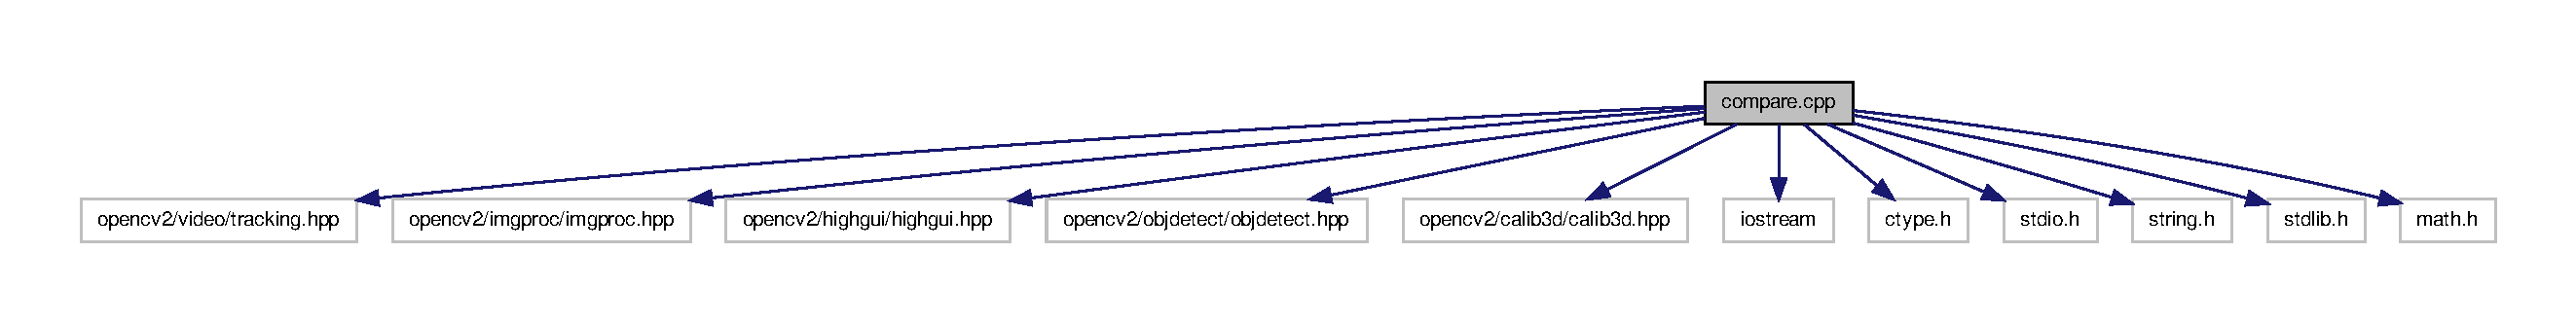
\includegraphics[width=350pt]{compare_8cpp__incl}
\end{center}
\end{figure}
\subsection*{Functions}
\begin{DoxyCompactItemize}
\item 
void \hyperlink{compare_8cpp_a9c549df82d21fa50db5e67bb16aad89d}{read\-\_\-from\-\_\-file} (string filename, vector$<$ Point $>$ \&\hyperlink{social__robot__onethread_8cpp_acb84e343c5602756e13a851a44128639}{rois})
\item 
void \hyperlink{compare_8cpp_aec5853a4c45d2d1017a5aa21353e588e}{write\-\_\-to\-\_\-file} (string filename, vector$<$ double $>$ \hyperlink{social__robot__onethread_8cpp_acb84e343c5602756e13a851a44128639}{rois}, double mse)
\item 
void \hyperlink{compare_8cpp_aa0c68124ea7a3fa23be6e78981ad3bdb}{create\-\_\-combine\-\_\-gt\-\_\-vector} (vector$<$ string $>$ filenames, vector$<$ vector$<$ Point $>$ $>$ \&total\-\_\-gt)
\item 
void \hyperlink{compare_8cpp_a0d619e8c70176657e1f4c8a73a105213}{gt\-\_\-tracking\-\_\-comparison} (vector$<$ Point $>$ gt, vector$<$ Point $>$tracking, string filename)
\item 
void \hyperlink{compare_8cpp_a97ee70a8770dc30d06c744b24eb2fcfc}{help} ()
\item 
int \hyperlink{compare_8cpp_a217dbf8b442f20279ea00b898af96f52}{main} (int argc, const char $\ast$$\ast$argv)
\end{DoxyCompactItemize}


\subsection{Function Documentation}
\hypertarget{compare_8cpp_aa0c68124ea7a3fa23be6e78981ad3bdb}{\index{compare.\-cpp@{compare.\-cpp}!create\-\_\-combine\-\_\-gt\-\_\-vector@{create\-\_\-combine\-\_\-gt\-\_\-vector}}
\index{create\-\_\-combine\-\_\-gt\-\_\-vector@{create\-\_\-combine\-\_\-gt\-\_\-vector}!compare.cpp@{compare.\-cpp}}
\subsubsection[{create\-\_\-combine\-\_\-gt\-\_\-vector}]{\setlength{\rightskip}{0pt plus 5cm}void create\-\_\-combine\-\_\-gt\-\_\-vector (
\begin{DoxyParamCaption}
\item[{vector$<$ string $>$}]{filenames, }
\item[{vector$<$ vector$<$ Point $>$ $>$ \&}]{total\-\_\-gt}
\end{DoxyParamCaption}
)}}\label{compare_8cpp_aa0c68124ea7a3fa23be6e78981ad3bdb}
\hypertarget{compare_8cpp_a0d619e8c70176657e1f4c8a73a105213}{\index{compare.\-cpp@{compare.\-cpp}!gt\-\_\-tracking\-\_\-comparison@{gt\-\_\-tracking\-\_\-comparison}}
\index{gt\-\_\-tracking\-\_\-comparison@{gt\-\_\-tracking\-\_\-comparison}!compare.cpp@{compare.\-cpp}}
\subsubsection[{gt\-\_\-tracking\-\_\-comparison}]{\setlength{\rightskip}{0pt plus 5cm}void gt\-\_\-tracking\-\_\-comparison (
\begin{DoxyParamCaption}
\item[{vector$<$ Point $>$}]{gt, }
\item[{vector$<$ Point $>$}]{tracking, }
\item[{string}]{filename}
\end{DoxyParamCaption}
)}}\label{compare_8cpp_a0d619e8c70176657e1f4c8a73a105213}
\hypertarget{compare_8cpp_a97ee70a8770dc30d06c744b24eb2fcfc}{\index{compare.\-cpp@{compare.\-cpp}!help@{help}}
\index{help@{help}!compare.cpp@{compare.\-cpp}}
\subsubsection[{help}]{\setlength{\rightskip}{0pt plus 5cm}void help (
\begin{DoxyParamCaption}
{}
\end{DoxyParamCaption}
)}}\label{compare_8cpp_a97ee70a8770dc30d06c744b24eb2fcfc}
\hypertarget{compare_8cpp_a217dbf8b442f20279ea00b898af96f52}{\index{compare.\-cpp@{compare.\-cpp}!main@{main}}
\index{main@{main}!compare.cpp@{compare.\-cpp}}
\subsubsection[{main}]{\setlength{\rightskip}{0pt plus 5cm}int main (
\begin{DoxyParamCaption}
\item[{int}]{argc, }
\item[{const char $\ast$$\ast$}]{argv}
\end{DoxyParamCaption}
)}}\label{compare_8cpp_a217dbf8b442f20279ea00b898af96f52}
\hypertarget{compare_8cpp_a9c549df82d21fa50db5e67bb16aad89d}{\index{compare.\-cpp@{compare.\-cpp}!read\-\_\-from\-\_\-file@{read\-\_\-from\-\_\-file}}
\index{read\-\_\-from\-\_\-file@{read\-\_\-from\-\_\-file}!compare.cpp@{compare.\-cpp}}
\subsubsection[{read\-\_\-from\-\_\-file}]{\setlength{\rightskip}{0pt plus 5cm}void read\-\_\-from\-\_\-file (
\begin{DoxyParamCaption}
\item[{string}]{filename, }
\item[{vector$<$ Point $>$ \&}]{rois}
\end{DoxyParamCaption}
)}}\label{compare_8cpp_a9c549df82d21fa50db5e67bb16aad89d}
This function reads from a .yaml file the coordinates of the center of R\-O\-I \begin{DoxyReturn}{Returns}

\end{DoxyReturn}

\begin{DoxyParams}{Parameters}
{\em file\-\_\-name} & A string file containing the input file \\
\hline
{\em rois} & A vector of Points containing the centers of R\-O\-I. \\
\hline
\end{DoxyParams}
\hypertarget{compare_8cpp_aec5853a4c45d2d1017a5aa21353e588e}{\index{compare.\-cpp@{compare.\-cpp}!write\-\_\-to\-\_\-file@{write\-\_\-to\-\_\-file}}
\index{write\-\_\-to\-\_\-file@{write\-\_\-to\-\_\-file}!compare.cpp@{compare.\-cpp}}
\subsubsection[{write\-\_\-to\-\_\-file}]{\setlength{\rightskip}{0pt plus 5cm}void write\-\_\-to\-\_\-file (
\begin{DoxyParamCaption}
\item[{string}]{filename, }
\item[{vector$<$ double $>$}]{rois, }
\item[{double}]{mse}
\end{DoxyParamCaption}
)}}\label{compare_8cpp_aec5853a4c45d2d1017a5aa21353e588e}
This function writes the distance and M\-S\-E between ground-\/truth and tracking results to a .yaml file \begin{DoxyReturn}{Returns}

\end{DoxyReturn}

\begin{DoxyParams}{Parameters}
{\em file\-\_\-name} & A string file containing the output file \\
\hline
{\em rois} & A vector of doubles containing the distances. \\
\hline
{\em mse} & The Mean Square Error. \\
\hline
\end{DoxyParams}

\hypertarget{compare__ground__truth_8cpp}{\section{compare\-\_\-ground\-\_\-truth.\-cpp File Reference}
\label{compare__ground__truth_8cpp}\index{compare\-\_\-ground\-\_\-truth.\-cpp@{compare\-\_\-ground\-\_\-truth.\-cpp}}
}
{\ttfamily \#include $<$opencv2/video/tracking.\-hpp$>$}\\*
{\ttfamily \#include $<$opencv2/imgproc/imgproc.\-hpp$>$}\\*
{\ttfamily \#include $<$opencv2/highgui/highgui.\-hpp$>$}\\*
{\ttfamily \#include $<$iostream$>$}\\*
{\ttfamily \#include $<$ctype.\-h$>$}\\*
{\ttfamily \#include $<$stdio.\-h$>$}\\*
{\ttfamily \#include $<$string.\-h$>$}\\*
{\ttfamily \#include $<$stdlib.\-h$>$}\\*
{\ttfamily \#include $<$math.\-h$>$}\\*
Include dependency graph for compare\-\_\-ground\-\_\-truth.\-cpp\-:\nopagebreak
\begin{figure}[H]
\begin{center}
\leavevmode
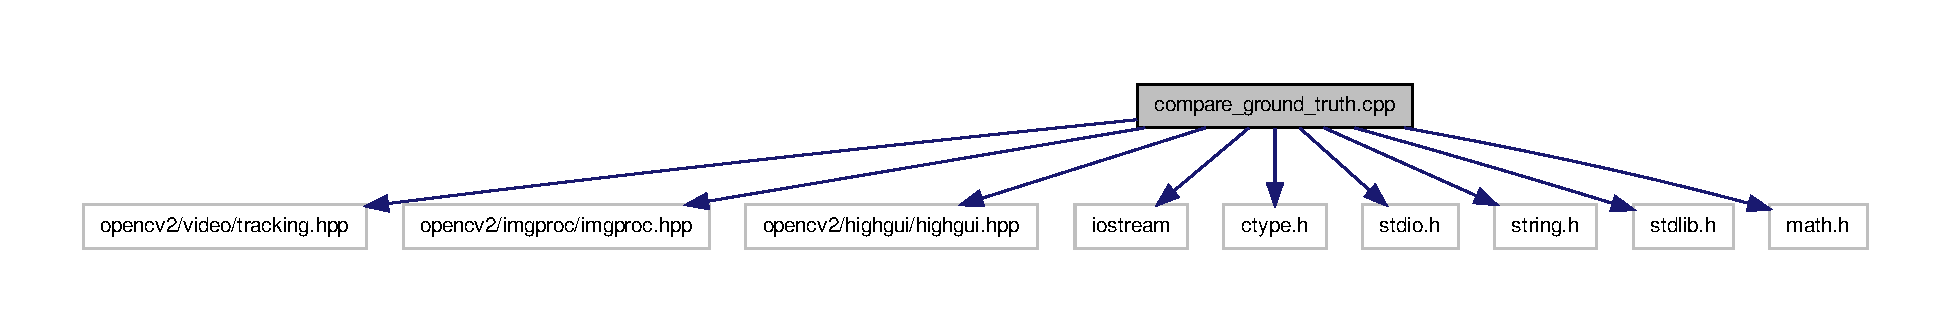
\includegraphics[width=350pt]{compare__ground__truth_8cpp__incl}
\end{center}
\end{figure}
\subsection*{Functions}
\begin{DoxyCompactItemize}
\item 
void \hyperlink{compare__ground__truth_8cpp_a9c549df82d21fa50db5e67bb16aad89d}{read\-\_\-from\-\_\-file} (string filename, vector$<$ Point $>$ \&\hyperlink{social__robot__onethread_8cpp_acb84e343c5602756e13a851a44128639}{rois})
\item 
void \hyperlink{compare__ground__truth_8cpp_aec5853a4c45d2d1017a5aa21353e588e}{write\-\_\-to\-\_\-file} (string filename, vector$<$ double $>$ \hyperlink{social__robot__onethread_8cpp_acb84e343c5602756e13a851a44128639}{rois}, double mse)
\item 
void \hyperlink{compare__ground__truth_8cpp_a97ee70a8770dc30d06c744b24eb2fcfc}{help} ()
\item 
int \hyperlink{compare__ground__truth_8cpp_a217dbf8b442f20279ea00b898af96f52}{main} (int argc, const char $\ast$$\ast$argv)
\end{DoxyCompactItemize}


\subsection{Function Documentation}
\hypertarget{compare__ground__truth_8cpp_a97ee70a8770dc30d06c744b24eb2fcfc}{\index{compare\-\_\-ground\-\_\-truth.\-cpp@{compare\-\_\-ground\-\_\-truth.\-cpp}!help@{help}}
\index{help@{help}!compare_ground_truth.cpp@{compare\-\_\-ground\-\_\-truth.\-cpp}}
\subsubsection[{help}]{\setlength{\rightskip}{0pt plus 5cm}void help (
\begin{DoxyParamCaption}
{}
\end{DoxyParamCaption}
)}}\label{compare__ground__truth_8cpp_a97ee70a8770dc30d06c744b24eb2fcfc}
\hypertarget{compare__ground__truth_8cpp_a217dbf8b442f20279ea00b898af96f52}{\index{compare\-\_\-ground\-\_\-truth.\-cpp@{compare\-\_\-ground\-\_\-truth.\-cpp}!main@{main}}
\index{main@{main}!compare_ground_truth.cpp@{compare\-\_\-ground\-\_\-truth.\-cpp}}
\subsubsection[{main}]{\setlength{\rightskip}{0pt plus 5cm}int main (
\begin{DoxyParamCaption}
\item[{int}]{argc, }
\item[{const char $\ast$$\ast$}]{argv}
\end{DoxyParamCaption}
)}}\label{compare__ground__truth_8cpp_a217dbf8b442f20279ea00b898af96f52}
\hypertarget{compare__ground__truth_8cpp_a9c549df82d21fa50db5e67bb16aad89d}{\index{compare\-\_\-ground\-\_\-truth.\-cpp@{compare\-\_\-ground\-\_\-truth.\-cpp}!read\-\_\-from\-\_\-file@{read\-\_\-from\-\_\-file}}
\index{read\-\_\-from\-\_\-file@{read\-\_\-from\-\_\-file}!compare_ground_truth.cpp@{compare\-\_\-ground\-\_\-truth.\-cpp}}
\subsubsection[{read\-\_\-from\-\_\-file}]{\setlength{\rightskip}{0pt plus 5cm}void read\-\_\-from\-\_\-file (
\begin{DoxyParamCaption}
\item[{string}]{filename, }
\item[{vector$<$ Point $>$ \&}]{rois}
\end{DoxyParamCaption}
)}}\label{compare__ground__truth_8cpp_a9c549df82d21fa50db5e67bb16aad89d}
This function reads from a .yaml file the coordinates of the center of R\-O\-I \begin{DoxyReturn}{Returns}

\end{DoxyReturn}

\begin{DoxyParams}{Parameters}
{\em file\-\_\-name} & A string file containing the input file \\
\hline
{\em rois} & A vector of Points containing the centers of R\-O\-I. \\
\hline
\end{DoxyParams}
\hypertarget{compare__ground__truth_8cpp_aec5853a4c45d2d1017a5aa21353e588e}{\index{compare\-\_\-ground\-\_\-truth.\-cpp@{compare\-\_\-ground\-\_\-truth.\-cpp}!write\-\_\-to\-\_\-file@{write\-\_\-to\-\_\-file}}
\index{write\-\_\-to\-\_\-file@{write\-\_\-to\-\_\-file}!compare_ground_truth.cpp@{compare\-\_\-ground\-\_\-truth.\-cpp}}
\subsubsection[{write\-\_\-to\-\_\-file}]{\setlength{\rightskip}{0pt plus 5cm}void write\-\_\-to\-\_\-file (
\begin{DoxyParamCaption}
\item[{string}]{filename, }
\item[{vector$<$ double $>$}]{rois, }
\item[{double}]{mse}
\end{DoxyParamCaption}
)}}\label{compare__ground__truth_8cpp_aec5853a4c45d2d1017a5aa21353e588e}
This function writes the distance and M\-S\-E between ground-\/truth and tracking results to a .yaml file \begin{DoxyReturn}{Returns}

\end{DoxyReturn}

\begin{DoxyParams}{Parameters}
{\em file\-\_\-name} & A string file containing the output file \\
\hline
{\em rois} & A vector of doubles containing the distances. \\
\hline
{\em mse} & The Mean Square Error. \\
\hline
\end{DoxyParams}

\hypertarget{condens_8cpp}{\section{condens.\-cpp File Reference}
\label{condens_8cpp}\index{condens.\-cpp@{condens.\-cpp}}
}
{\ttfamily \#include \char`\"{}condens.\-h\char`\"{}}\\*
Include dependency graph for condens.\-cpp\-:\nopagebreak
\begin{figure}[H]
\begin{center}
\leavevmode
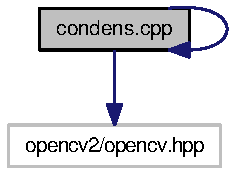
\includegraphics[width=186pt]{condens_8cpp__incl}
\end{center}
\end{figure}
\subsection*{Typedefs}
\begin{DoxyCompactItemize}
\item 
typedef unsigned int \hyperlink{condens_8cpp_a91ad9478d81a7aaf2593e8d9c3d06a14}{uint}
\end{DoxyCompactItemize}


\subsection{Typedef Documentation}
\hypertarget{condens_8cpp_a91ad9478d81a7aaf2593e8d9c3d06a14}{\index{condens.\-cpp@{condens.\-cpp}!uint@{uint}}
\index{uint@{uint}!condens.cpp@{condens.\-cpp}}
\subsubsection[{uint}]{\setlength{\rightskip}{0pt plus 5cm}typedef unsigned int {\bf uint}}}\label{condens_8cpp_a91ad9478d81a7aaf2593e8d9c3d06a14}

\hypertarget{condens_8h}{
\section{condens.h File Reference}
\label{condens_8h}\index{condens.h@{condens.h}}
}
{\ttfamily \#include $<$opencv2/opencv.hpp$>$}\par
Include dependency graph for condens.h:\nopagebreak
\begin{figure}[H]
\begin{center}
\leavevmode
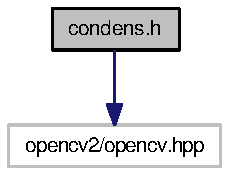
\includegraphics[width=73pt]{condens_8h__incl}
\end{center}
\end{figure}
This graph shows which files directly or indirectly include this file:\nopagebreak
\begin{figure}[H]
\begin{center}
\leavevmode
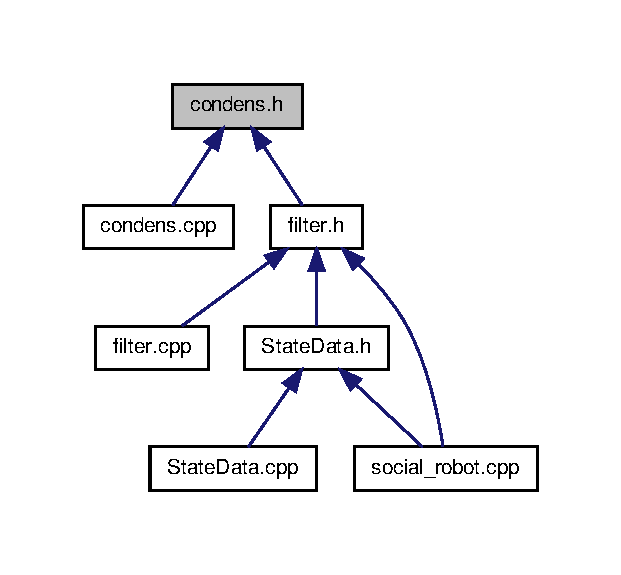
\includegraphics[width=402pt]{condens_8h__dep__incl}
\end{center}
\end{figure}
\subsection*{Data Structures}
\begin{DoxyCompactItemize}
\item 
class \hyperlink{classConDensation}{ConDensation}
\end{DoxyCompactItemize}

\hypertarget{create__ground__truth_8cpp}{\section{create\-\_\-ground\-\_\-truth.\-cpp File Reference}
\label{create__ground__truth_8cpp}\index{create\-\_\-ground\-\_\-truth.\-cpp@{create\-\_\-ground\-\_\-truth.\-cpp}}
}
{\ttfamily \#include $<$opencv2/highgui/highgui.\-hpp$>$}\\*
{\ttfamily \#include $<$iostream$>$}\\*
{\ttfamily \#include $<$ctype.\-h$>$}\\*
{\ttfamily \#include $<$stdio.\-h$>$}\\*
{\ttfamily \#include $<$string.\-h$>$}\\*
Include dependency graph for create\-\_\-ground\-\_\-truth.\-cpp\-:\nopagebreak
\begin{figure}[H]
\begin{center}
\leavevmode
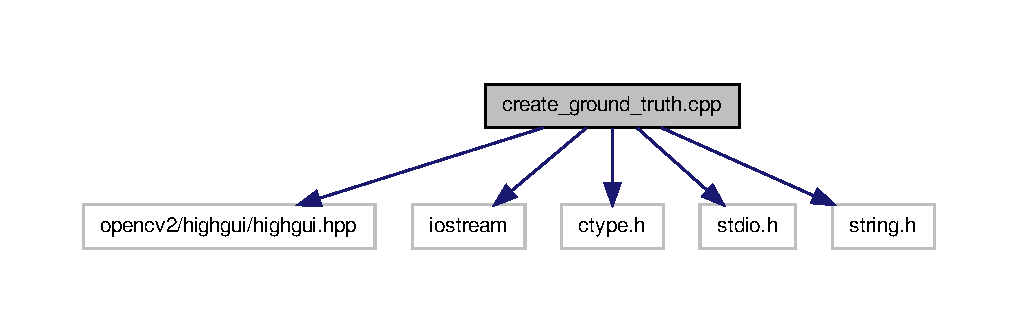
\includegraphics[width=350pt]{create__ground__truth_8cpp__incl}
\end{center}
\end{figure}
\subsection*{Functions}
\begin{DoxyCompactItemize}
\item 
void \hyperlink{create__ground__truth_8cpp_a6c81aa00b4dcf0cbae98a14c37683ed9}{on\-Mouse} (int event, int x, int y, int, void $\ast$)
\item 
void \hyperlink{create__ground__truth_8cpp_aebb0550776d5f429fb7a03f7574545ec}{write\-\_\-results\-\_\-to\-\_\-file} (string \hyperlink{social__robot_8cpp_a755d42f2e9c635ce2213e0efad62b796}{file\-\_\-name}, vector$<$ Rect $>$ \hyperlink{social__robot__onethread_8cpp_acb84e343c5602756e13a851a44128639}{rois})
\item 
Rect \hyperlink{create__ground__truth_8cpp_aaa36eba0517e48e70129a66bea3b50b5}{check\-\_\-boundaries} (Rect window)
\item 
void \hyperlink{create__ground__truth_8cpp_a97ee70a8770dc30d06c744b24eb2fcfc}{help} ()
\item 
int \hyperlink{create__ground__truth_8cpp_a217dbf8b442f20279ea00b898af96f52}{main} (int argc, const char $\ast$$\ast$argv)
\end{DoxyCompactItemize}
\subsection*{Variables}
\begin{DoxyCompactItemize}
\item 
Mat \hyperlink{create__ground__truth_8cpp_aabb27b8973575043030df51be47cd24a}{image}
\item 
int \hyperlink{create__ground__truth_8cpp_a88f176e4e65e22a17093a8cd24003a66}{track\-Object} = 0
\item 
int \hyperlink{create__ground__truth_8cpp_a13f77b252237844d7b8b6e3c3047fe50}{skip} = 0
\item 
bool \hyperlink{create__ground__truth_8cpp_a71a276a0dc4ef6aa35740b58f10bcb39}{select\-Object} = false
\item 
bool \hyperlink{create__ground__truth_8cpp_a1692a08e70fa31c61e66b87cdb53dbd5}{is\-\_\-first\-\_\-frame} = true
\item 
Point \hyperlink{create__ground__truth_8cpp_a903d0d8820c696aaa1170c50deb3633f}{origin}
\item 
Rect \hyperlink{create__ground__truth_8cpp_a15633c47538e3790df1e008a7f6dbfea}{selection}
\item 
vector$<$ Rect $>$ \hyperlink{create__ground__truth_8cpp_acee6f4679f3fb598d19b3dcdd30c04a3}{to\-\_\-be\-\_\-saved}
\end{DoxyCompactItemize}


\subsection{Function Documentation}
\hypertarget{create__ground__truth_8cpp_aaa36eba0517e48e70129a66bea3b50b5}{\index{create\-\_\-ground\-\_\-truth.\-cpp@{create\-\_\-ground\-\_\-truth.\-cpp}!check\-\_\-boundaries@{check\-\_\-boundaries}}
\index{check\-\_\-boundaries@{check\-\_\-boundaries}!create_ground_truth.cpp@{create\-\_\-ground\-\_\-truth.\-cpp}}
\subsubsection[{check\-\_\-boundaries}]{\setlength{\rightskip}{0pt plus 5cm}Rect check\-\_\-boundaries (
\begin{DoxyParamCaption}
\item[{Rect}]{window}
\end{DoxyParamCaption}
)}}\label{create__ground__truth_8cpp_aaa36eba0517e48e70129a66bea3b50b5}
This function checks if the R\-O\-I has excedded the dimensions of the image \begin{DoxyReturn}{Returns}

\end{DoxyReturn}

\begin{DoxyParams}{Parameters}
{\em window} & A Rect containing the R\-O\-I. \\
\hline
\end{DoxyParams}
\hypertarget{create__ground__truth_8cpp_a97ee70a8770dc30d06c744b24eb2fcfc}{\index{create\-\_\-ground\-\_\-truth.\-cpp@{create\-\_\-ground\-\_\-truth.\-cpp}!help@{help}}
\index{help@{help}!create_ground_truth.cpp@{create\-\_\-ground\-\_\-truth.\-cpp}}
\subsubsection[{help}]{\setlength{\rightskip}{0pt plus 5cm}void help (
\begin{DoxyParamCaption}
{}
\end{DoxyParamCaption}
)}}\label{create__ground__truth_8cpp_a97ee70a8770dc30d06c744b24eb2fcfc}
\hypertarget{create__ground__truth_8cpp_a217dbf8b442f20279ea00b898af96f52}{\index{create\-\_\-ground\-\_\-truth.\-cpp@{create\-\_\-ground\-\_\-truth.\-cpp}!main@{main}}
\index{main@{main}!create_ground_truth.cpp@{create\-\_\-ground\-\_\-truth.\-cpp}}
\subsubsection[{main}]{\setlength{\rightskip}{0pt plus 5cm}int main (
\begin{DoxyParamCaption}
\item[{int}]{argc, }
\item[{const char $\ast$$\ast$}]{argv}
\end{DoxyParamCaption}
)}}\label{create__ground__truth_8cpp_a217dbf8b442f20279ea00b898af96f52}
\hypertarget{create__ground__truth_8cpp_a6c81aa00b4dcf0cbae98a14c37683ed9}{\index{create\-\_\-ground\-\_\-truth.\-cpp@{create\-\_\-ground\-\_\-truth.\-cpp}!on\-Mouse@{on\-Mouse}}
\index{on\-Mouse@{on\-Mouse}!create_ground_truth.cpp@{create\-\_\-ground\-\_\-truth.\-cpp}}
\subsubsection[{on\-Mouse}]{\setlength{\rightskip}{0pt plus 5cm}void on\-Mouse (
\begin{DoxyParamCaption}
\item[{int}]{event, }
\item[{int}]{x, }
\item[{int}]{y, }
\item[{int}]{, }
\item[{void $\ast$}]{}
\end{DoxyParamCaption}
)}}\label{create__ground__truth_8cpp_a6c81aa00b4dcf0cbae98a14c37683ed9}
\hypertarget{create__ground__truth_8cpp_aebb0550776d5f429fb7a03f7574545ec}{\index{create\-\_\-ground\-\_\-truth.\-cpp@{create\-\_\-ground\-\_\-truth.\-cpp}!write\-\_\-results\-\_\-to\-\_\-file@{write\-\_\-results\-\_\-to\-\_\-file}}
\index{write\-\_\-results\-\_\-to\-\_\-file@{write\-\_\-results\-\_\-to\-\_\-file}!create_ground_truth.cpp@{create\-\_\-ground\-\_\-truth.\-cpp}}
\subsubsection[{write\-\_\-results\-\_\-to\-\_\-file}]{\setlength{\rightskip}{0pt plus 5cm}void write\-\_\-results\-\_\-to\-\_\-file (
\begin{DoxyParamCaption}
\item[{string}]{file\-\_\-name, }
\item[{vector$<$ Rect $>$}]{rois}
\end{DoxyParamCaption}
)}}\label{create__ground__truth_8cpp_aebb0550776d5f429fb7a03f7574545ec}
This function writes the coordinates of a rectangle to a .yaml file \begin{DoxyReturn}{Returns}

\end{DoxyReturn}

\begin{DoxyParams}{Parameters}
{\em file\-\_\-name} & A string file containing the output file \\
\hline
{\em roi} & A vector of rectangles containing the R\-O\-I. \\
\hline
\end{DoxyParams}


\subsection{Variable Documentation}
\hypertarget{create__ground__truth_8cpp_aabb27b8973575043030df51be47cd24a}{\index{create\-\_\-ground\-\_\-truth.\-cpp@{create\-\_\-ground\-\_\-truth.\-cpp}!image@{image}}
\index{image@{image}!create_ground_truth.cpp@{create\-\_\-ground\-\_\-truth.\-cpp}}
\subsubsection[{image}]{\setlength{\rightskip}{0pt plus 5cm}Mat image}}\label{create__ground__truth_8cpp_aabb27b8973575043030df51be47cd24a}
\hypertarget{create__ground__truth_8cpp_a1692a08e70fa31c61e66b87cdb53dbd5}{\index{create\-\_\-ground\-\_\-truth.\-cpp@{create\-\_\-ground\-\_\-truth.\-cpp}!is\-\_\-first\-\_\-frame@{is\-\_\-first\-\_\-frame}}
\index{is\-\_\-first\-\_\-frame@{is\-\_\-first\-\_\-frame}!create_ground_truth.cpp@{create\-\_\-ground\-\_\-truth.\-cpp}}
\subsubsection[{is\-\_\-first\-\_\-frame}]{\setlength{\rightskip}{0pt plus 5cm}bool is\-\_\-first\-\_\-frame = true}}\label{create__ground__truth_8cpp_a1692a08e70fa31c61e66b87cdb53dbd5}
\hypertarget{create__ground__truth_8cpp_a903d0d8820c696aaa1170c50deb3633f}{\index{create\-\_\-ground\-\_\-truth.\-cpp@{create\-\_\-ground\-\_\-truth.\-cpp}!origin@{origin}}
\index{origin@{origin}!create_ground_truth.cpp@{create\-\_\-ground\-\_\-truth.\-cpp}}
\subsubsection[{origin}]{\setlength{\rightskip}{0pt plus 5cm}Point origin}}\label{create__ground__truth_8cpp_a903d0d8820c696aaa1170c50deb3633f}
\hypertarget{create__ground__truth_8cpp_a15633c47538e3790df1e008a7f6dbfea}{\index{create\-\_\-ground\-\_\-truth.\-cpp@{create\-\_\-ground\-\_\-truth.\-cpp}!selection@{selection}}
\index{selection@{selection}!create_ground_truth.cpp@{create\-\_\-ground\-\_\-truth.\-cpp}}
\subsubsection[{selection}]{\setlength{\rightskip}{0pt plus 5cm}Rect selection}}\label{create__ground__truth_8cpp_a15633c47538e3790df1e008a7f6dbfea}
\hypertarget{create__ground__truth_8cpp_a71a276a0dc4ef6aa35740b58f10bcb39}{\index{create\-\_\-ground\-\_\-truth.\-cpp@{create\-\_\-ground\-\_\-truth.\-cpp}!select\-Object@{select\-Object}}
\index{select\-Object@{select\-Object}!create_ground_truth.cpp@{create\-\_\-ground\-\_\-truth.\-cpp}}
\subsubsection[{select\-Object}]{\setlength{\rightskip}{0pt plus 5cm}bool select\-Object = false}}\label{create__ground__truth_8cpp_a71a276a0dc4ef6aa35740b58f10bcb39}
\hypertarget{create__ground__truth_8cpp_a13f77b252237844d7b8b6e3c3047fe50}{\index{create\-\_\-ground\-\_\-truth.\-cpp@{create\-\_\-ground\-\_\-truth.\-cpp}!skip@{skip}}
\index{skip@{skip}!create_ground_truth.cpp@{create\-\_\-ground\-\_\-truth.\-cpp}}
\subsubsection[{skip}]{\setlength{\rightskip}{0pt plus 5cm}int skip = 0}}\label{create__ground__truth_8cpp_a13f77b252237844d7b8b6e3c3047fe50}
\hypertarget{create__ground__truth_8cpp_acee6f4679f3fb598d19b3dcdd30c04a3}{\index{create\-\_\-ground\-\_\-truth.\-cpp@{create\-\_\-ground\-\_\-truth.\-cpp}!to\-\_\-be\-\_\-saved@{to\-\_\-be\-\_\-saved}}
\index{to\-\_\-be\-\_\-saved@{to\-\_\-be\-\_\-saved}!create_ground_truth.cpp@{create\-\_\-ground\-\_\-truth.\-cpp}}
\subsubsection[{to\-\_\-be\-\_\-saved}]{\setlength{\rightskip}{0pt plus 5cm}vector$<$Rect$>$ to\-\_\-be\-\_\-saved}}\label{create__ground__truth_8cpp_acee6f4679f3fb598d19b3dcdd30c04a3}
\hypertarget{create__ground__truth_8cpp_a88f176e4e65e22a17093a8cd24003a66}{\index{create\-\_\-ground\-\_\-truth.\-cpp@{create\-\_\-ground\-\_\-truth.\-cpp}!track\-Object@{track\-Object}}
\index{track\-Object@{track\-Object}!create_ground_truth.cpp@{create\-\_\-ground\-\_\-truth.\-cpp}}
\subsubsection[{track\-Object}]{\setlength{\rightskip}{0pt plus 5cm}int track\-Object = 0}}\label{create__ground__truth_8cpp_a88f176e4e65e22a17093a8cd24003a66}

\hypertarget{CvUtils_8cpp}{\section{Cv\-Utils.\-cpp File Reference}
\label{CvUtils_8cpp}\index{Cv\-Utils.\-cpp@{Cv\-Utils.\-cpp}}
}
{\ttfamily \#include \char`\"{}Cv\-Utils.\-h\char`\"{}}\\*
Include dependency graph for Cv\-Utils.\-cpp\-:
\nopagebreak
\begin{figure}[H]
\begin{center}
\leavevmode
\includegraphics[width=350pt]{CvUtils_8cpp__incl}
\end{center}
\end{figure}

\hypertarget{CvUtils_8h}{
\section{CvUtils.h File Reference}
\label{CvUtils_8h}\index{CvUtils.h@{CvUtils.h}}
}
{\ttfamily \#include $<$opencv2/core/core.hpp$>$}\par
{\ttfamily \#include $<$opencv2/imgproc/imgproc.hpp$>$}\par
{\ttfamily \#include $<$opencv2/highgui/highgui.hpp$>$}\par
{\ttfamily \#include $<$opencv2/objdetect/objdetect.hpp$>$}\par
{\ttfamily \#include $<$iostream$>$}\par
{\ttfamily \#include $<$vector$>$}\par
{\ttfamily \#include \char`\"{}particle\_\-filter/StateData.h\char`\"{}}\par
Include dependency graph for CvUtils.h:\nopagebreak
\begin{figure}[H]
\begin{center}
\leavevmode
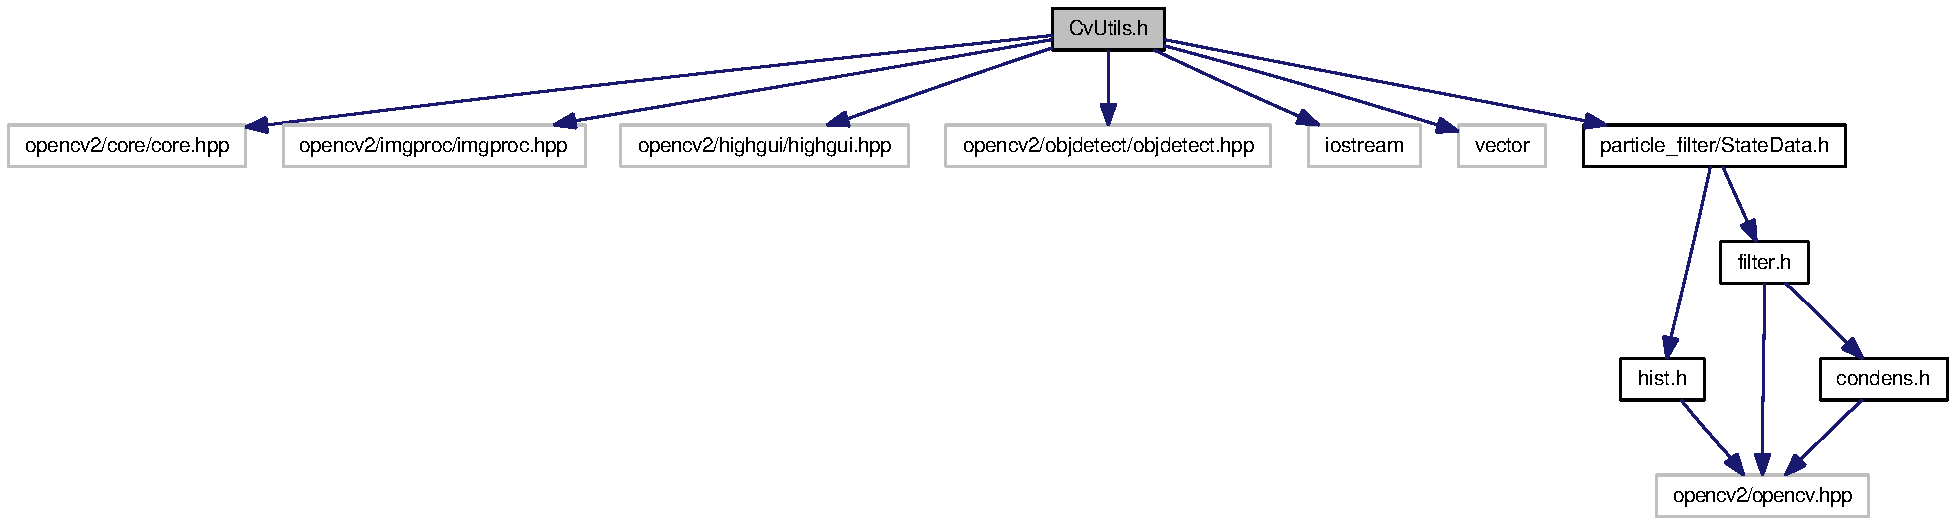
\includegraphics[width=420pt]{CvUtils_8h__incl}
\end{center}
\end{figure}
This graph shows which files directly or indirectly include this file:\nopagebreak
\begin{figure}[H]
\begin{center}
\leavevmode
\includegraphics[width=404pt]{CvUtils_8h__dep__incl}
\end{center}
\end{figure}
\subsection*{Data Structures}
\begin{DoxyCompactItemize}
\item 
class \hyperlink{classCvUtils}{CvUtils}
\begin{DoxyCompactList}\small\item\em This class contains useful functions for the image processing part. \item\end{DoxyCompactList}\end{DoxyCompactItemize}
\subsection*{Variables}
\begin{DoxyCompactItemize}
\item 
const Scalar \hyperlink{CvUtils_8h_a5127585a7c9e4bb80223ec9726c1d673}{RED} = Scalar ( 0, 0, 255 )
\item 
const Scalar \hyperlink{CvUtils_8h_a0e9bb5eea6e281c85d700124508dc137}{BLUE} = Scalar ( 255, 0, 0 )
\item 
const Scalar \hyperlink{CvUtils_8h_a814b97409628205acc4dbc39df04f7db}{GREEN} = Scalar ( 0, 255, 0 )
\item 
const Scalar \hyperlink{CvUtils_8h_a1f6da7b8c88800abc79ba4db1624f070}{CYAN} = Scalar ( 255, 255, 0 )
\item 
const Scalar \hyperlink{CvUtils_8h_a87dc5f5284a74230c0276ea03bd91726}{MAGENTA} = Scalar ( 255, 0, 255 )
\item 
const Scalar \hyperlink{CvUtils_8h_a2ba3d7c50aaa32291b634d66f127b197}{YELLOW} = Scalar ( 0, 255, 255 )
\item 
const Scalar \hyperlink{CvUtils_8h_a7e988685d36ceb4ddcc84fe9a5f03664}{WHITE} = Scalar ( 255, 255, 255 )
\item 
const Scalar \hyperlink{CvUtils_8h_a6a062c3d7c59f34957d22f8269d7d1f2}{BLACK} = Scalar ( 0, 0, 0 )
\end{DoxyCompactItemize}


\subsection{Variable Documentation}
\hypertarget{CvUtils_8h_a6a062c3d7c59f34957d22f8269d7d1f2}{
\index{CvUtils.h@{CvUtils.h}!BLACK@{BLACK}}
\index{BLACK@{BLACK}!CvUtils.h@{CvUtils.h}}
\subsubsection[{BLACK}]{\setlength{\rightskip}{0pt plus 5cm}const Scalar {\bf BLACK} = Scalar ( 0, 0, 0 )}}
\label{CvUtils_8h_a6a062c3d7c59f34957d22f8269d7d1f2}
\hypertarget{CvUtils_8h_a0e9bb5eea6e281c85d700124508dc137}{
\index{CvUtils.h@{CvUtils.h}!BLUE@{BLUE}}
\index{BLUE@{BLUE}!CvUtils.h@{CvUtils.h}}
\subsubsection[{BLUE}]{\setlength{\rightskip}{0pt plus 5cm}const Scalar {\bf BLUE} = Scalar ( 255, 0, 0 )}}
\label{CvUtils_8h_a0e9bb5eea6e281c85d700124508dc137}
\hypertarget{CvUtils_8h_a1f6da7b8c88800abc79ba4db1624f070}{
\index{CvUtils.h@{CvUtils.h}!CYAN@{CYAN}}
\index{CYAN@{CYAN}!CvUtils.h@{CvUtils.h}}
\subsubsection[{CYAN}]{\setlength{\rightskip}{0pt plus 5cm}const Scalar {\bf CYAN} = Scalar ( 255, 255, 0 )}}
\label{CvUtils_8h_a1f6da7b8c88800abc79ba4db1624f070}
\hypertarget{CvUtils_8h_a814b97409628205acc4dbc39df04f7db}{
\index{CvUtils.h@{CvUtils.h}!GREEN@{GREEN}}
\index{GREEN@{GREEN}!CvUtils.h@{CvUtils.h}}
\subsubsection[{GREEN}]{\setlength{\rightskip}{0pt plus 5cm}const Scalar {\bf GREEN} = Scalar ( 0, 255, 0 )}}
\label{CvUtils_8h_a814b97409628205acc4dbc39df04f7db}
\hypertarget{CvUtils_8h_a87dc5f5284a74230c0276ea03bd91726}{
\index{CvUtils.h@{CvUtils.h}!MAGENTA@{MAGENTA}}
\index{MAGENTA@{MAGENTA}!CvUtils.h@{CvUtils.h}}
\subsubsection[{MAGENTA}]{\setlength{\rightskip}{0pt plus 5cm}const Scalar {\bf MAGENTA} = Scalar ( 255, 0, 255 )}}
\label{CvUtils_8h_a87dc5f5284a74230c0276ea03bd91726}
\hypertarget{CvUtils_8h_a5127585a7c9e4bb80223ec9726c1d673}{
\index{CvUtils.h@{CvUtils.h}!RED@{RED}}
\index{RED@{RED}!CvUtils.h@{CvUtils.h}}
\subsubsection[{RED}]{\setlength{\rightskip}{0pt plus 5cm}const Scalar {\bf RED} = Scalar ( 0, 0, 255 )}}
\label{CvUtils_8h_a5127585a7c9e4bb80223ec9726c1d673}
\hypertarget{CvUtils_8h_a7e988685d36ceb4ddcc84fe9a5f03664}{
\index{CvUtils.h@{CvUtils.h}!WHITE@{WHITE}}
\index{WHITE@{WHITE}!CvUtils.h@{CvUtils.h}}
\subsubsection[{WHITE}]{\setlength{\rightskip}{0pt plus 5cm}const Scalar {\bf WHITE} = Scalar ( 255, 255, 255 )}}
\label{CvUtils_8h_a7e988685d36ceb4ddcc84fe9a5f03664}
\hypertarget{CvUtils_8h_a2ba3d7c50aaa32291b634d66f127b197}{
\index{CvUtils.h@{CvUtils.h}!YELLOW@{YELLOW}}
\index{YELLOW@{YELLOW}!CvUtils.h@{CvUtils.h}}
\subsubsection[{YELLOW}]{\setlength{\rightskip}{0pt plus 5cm}const Scalar {\bf YELLOW} = Scalar ( 0, 255, 255 )}}
\label{CvUtils_8h_a2ba3d7c50aaa32291b634d66f127b197}

\hypertarget{DepthFaceDetector_8cpp}{\section{Depth\-Face\-Detector.\-cpp File Reference}
\label{DepthFaceDetector_8cpp}\index{Depth\-Face\-Detector.\-cpp@{Depth\-Face\-Detector.\-cpp}}
}
{\ttfamily \#include \char`\"{}Depth\-Face\-Detector.\-h\char`\"{}}\\*
{\ttfamily \#include \char`\"{}Cv\-Utils.\-h\char`\"{}}\\*
{\ttfamily \#include $<$ros/package.\-h$>$}\\*
Include dependency graph for Depth\-Face\-Detector.\-cpp\-:
\nopagebreak
\begin{figure}[H]
\begin{center}
\leavevmode
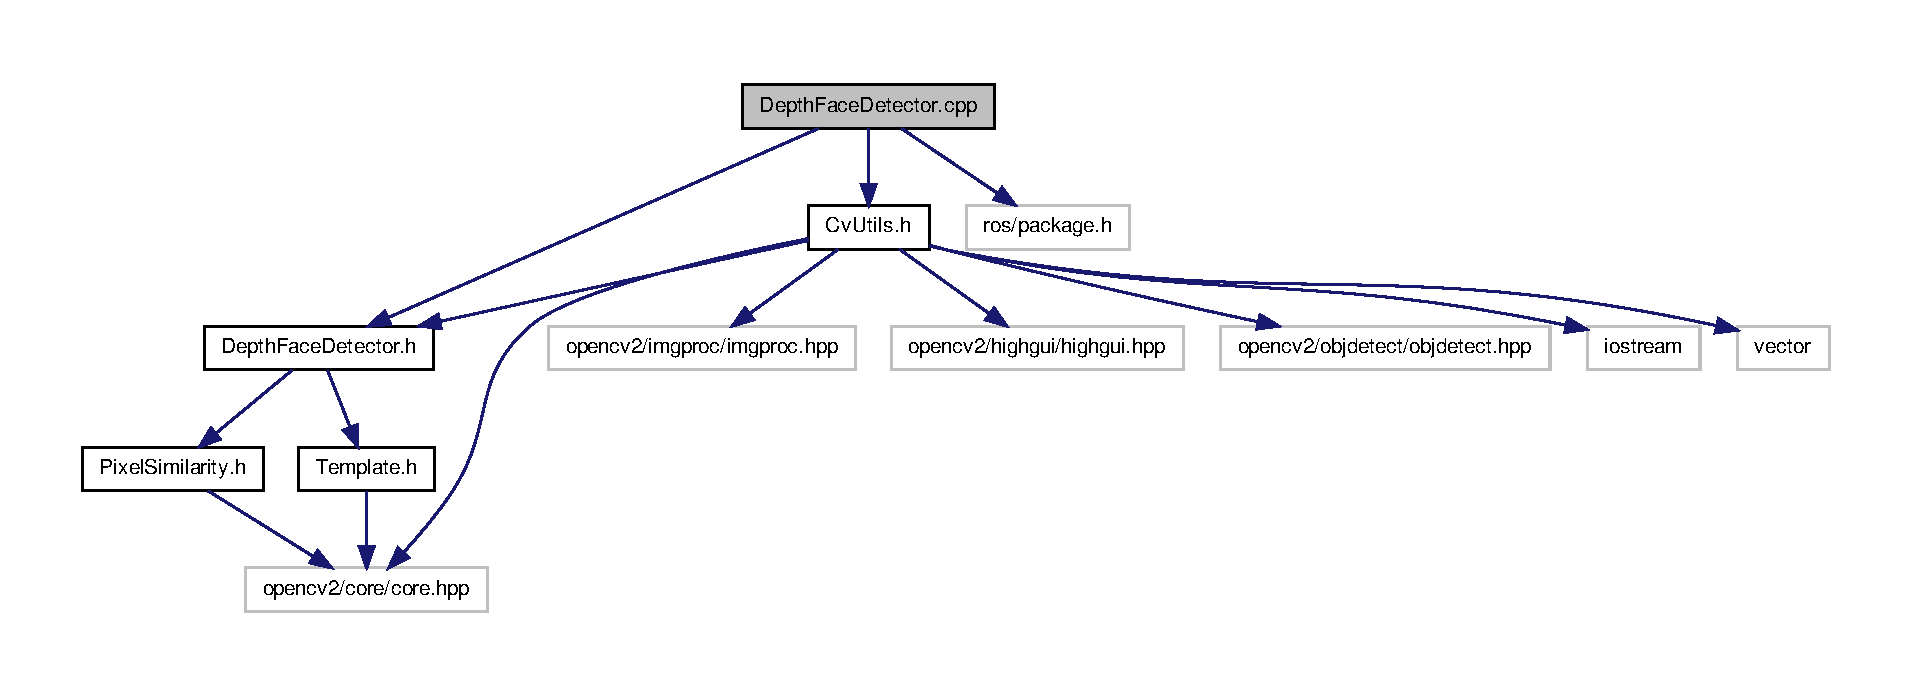
\includegraphics[width=350pt]{DepthFaceDetector_8cpp__incl}
\end{center}
\end{figure}
\subsection*{Macros}
\begin{DoxyCompactItemize}
\item 
\#define \hyperlink{DepthFaceDetector_8cpp_a2684f228d7751700fd20e4c4d5b0fe1a}{M\-O\-R\-P\-H\-\_\-\-S\-I\-Z\-E}~Size ( 11, 11 )
\end{DoxyCompactItemize}
\subsection*{Variables}
\begin{DoxyCompactItemize}
\item 
\hyperlink{classCvUtils}{Cv\-Utils} \hyperlink{DepthFaceDetector_8cpp_a199b98558819a161d93892eb6d1f766d}{cv\-\_\-utils}
\end{DoxyCompactItemize}


\subsection{Macro Definition Documentation}
\hypertarget{DepthFaceDetector_8cpp_a2684f228d7751700fd20e4c4d5b0fe1a}{\index{Depth\-Face\-Detector.\-cpp@{Depth\-Face\-Detector.\-cpp}!M\-O\-R\-P\-H\-\_\-\-S\-I\-Z\-E@{M\-O\-R\-P\-H\-\_\-\-S\-I\-Z\-E}}
\index{M\-O\-R\-P\-H\-\_\-\-S\-I\-Z\-E@{M\-O\-R\-P\-H\-\_\-\-S\-I\-Z\-E}!DepthFaceDetector.cpp@{Depth\-Face\-Detector.\-cpp}}
\subsubsection[{M\-O\-R\-P\-H\-\_\-\-S\-I\-Z\-E}]{\setlength{\rightskip}{0pt plus 5cm}\#define M\-O\-R\-P\-H\-\_\-\-S\-I\-Z\-E~Size ( 11, 11 )}}\label{DepthFaceDetector_8cpp_a2684f228d7751700fd20e4c4d5b0fe1a}


\subsection{Variable Documentation}
\hypertarget{DepthFaceDetector_8cpp_a199b98558819a161d93892eb6d1f766d}{\index{Depth\-Face\-Detector.\-cpp@{Depth\-Face\-Detector.\-cpp}!cv\-\_\-utils@{cv\-\_\-utils}}
\index{cv\-\_\-utils@{cv\-\_\-utils}!DepthFaceDetector.cpp@{Depth\-Face\-Detector.\-cpp}}
\subsubsection[{cv\-\_\-utils}]{\setlength{\rightskip}{0pt plus 5cm}{\bf Cv\-Utils} cv\-\_\-utils}}\label{DepthFaceDetector_8cpp_a199b98558819a161d93892eb6d1f766d}

\hypertarget{DepthFaceDetector_8h}{\section{Depth\-Face\-Detector.\-h File Reference}
\label{DepthFaceDetector_8h}\index{Depth\-Face\-Detector.\-h@{Depth\-Face\-Detector.\-h}}
}
{\ttfamily \#include \char`\"{}Pixel\-Similarity.\-h\char`\"{}}\\*
{\ttfamily \#include \char`\"{}Template.\-h\char`\"{}}\\*
Include dependency graph for Depth\-Face\-Detector.\-h\-:\nopagebreak
\begin{figure}[H]
\begin{center}
\leavevmode
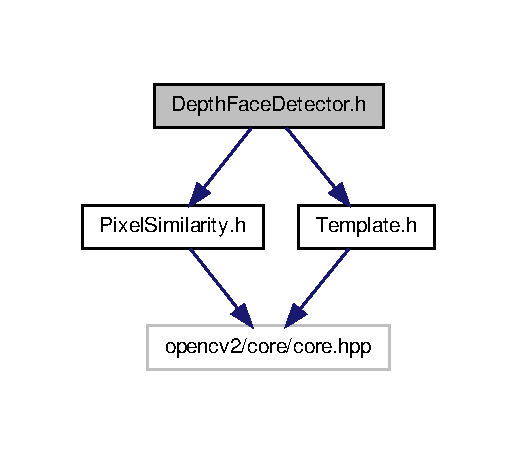
\includegraphics[width=248pt]{DepthFaceDetector_8h__incl}
\end{center}
\end{figure}
This graph shows which files directly or indirectly include this file\-:\nopagebreak
\begin{figure}[H]
\begin{center}
\leavevmode
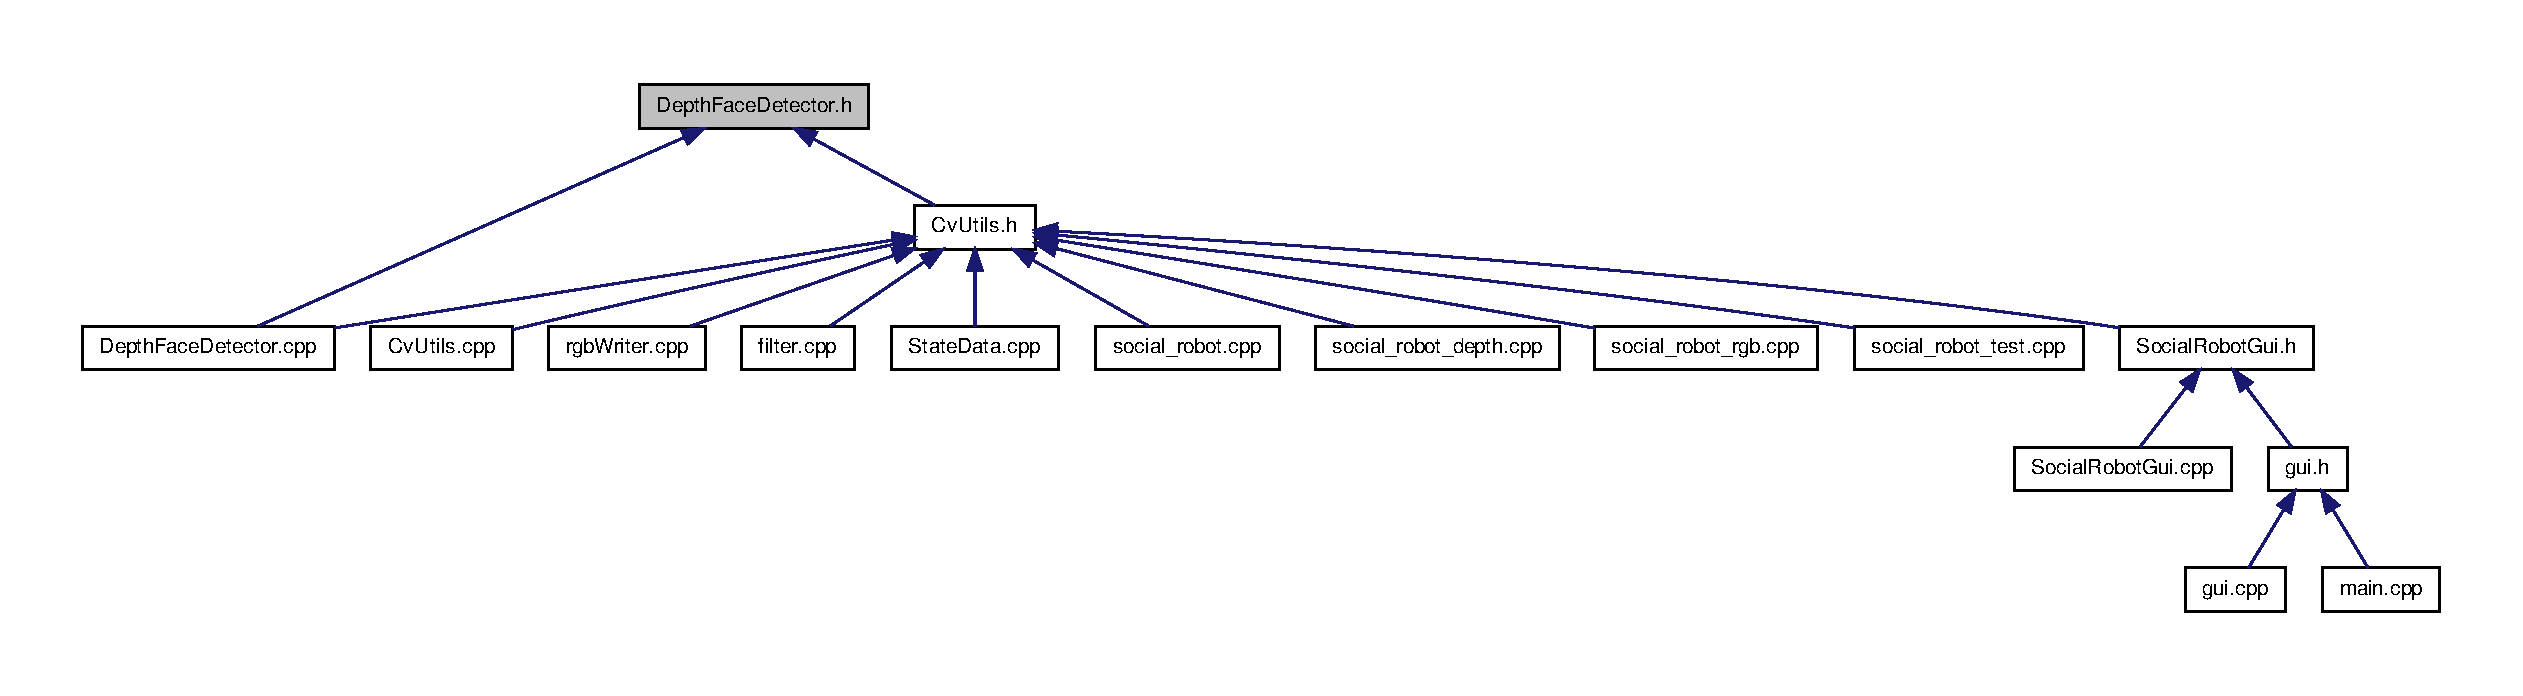
\includegraphics[width=350pt]{DepthFaceDetector_8h__dep__incl}
\end{center}
\end{figure}
\subsection*{Data Structures}
\begin{DoxyCompactItemize}
\item 
class \hyperlink{classDepthFaceDetector}{Depth\-Face\-Detector}
\end{DoxyCompactItemize}

\hypertarget{filter_8cpp}{\section{filter.\-cpp File Reference}
\label{filter_8cpp}\index{filter.\-cpp@{filter.\-cpp}}
}
{\ttfamily \#include \char`\"{}filter.\-h\char`\"{}}\\*
{\ttfamily \#include \char`\"{}hist.\-h\char`\"{}}\\*
{\ttfamily \#include \char`\"{}../\-Cv\-Utils.\-h\char`\"{}}\\*
{\ttfamily \#include $<$iostream$>$}\\*
Include dependency graph for filter.\-cpp\-:
\nopagebreak
\begin{figure}[H]
\begin{center}
\leavevmode
\includegraphics[width=350pt]{filter_8cpp__incl}
\end{center}
\end{figure}
\subsection*{Typedefs}
\begin{DoxyCompactItemize}
\item 
typedef unsigned int \hyperlink{filter_8cpp_a91ad9478d81a7aaf2593e8d9c3d06a14}{uint}
\end{DoxyCompactItemize}
\subsection*{Variables}
\begin{DoxyCompactItemize}
\item 
\hyperlink{classCvUtils}{Cv\-Utils} \hyperlink{filter_8cpp_a199b98558819a161d93892eb6d1f766d}{cv\-\_\-utils}
\end{DoxyCompactItemize}


\subsection{Typedef Documentation}
\hypertarget{filter_8cpp_a91ad9478d81a7aaf2593e8d9c3d06a14}{\index{filter.\-cpp@{filter.\-cpp}!uint@{uint}}
\index{uint@{uint}!filter.cpp@{filter.\-cpp}}
\subsubsection[{uint}]{\setlength{\rightskip}{0pt plus 5cm}typedef unsigned int {\bf uint}}}\label{filter_8cpp_a91ad9478d81a7aaf2593e8d9c3d06a14}


\subsection{Variable Documentation}
\hypertarget{filter_8cpp_a199b98558819a161d93892eb6d1f766d}{\index{filter.\-cpp@{filter.\-cpp}!cv\-\_\-utils@{cv\-\_\-utils}}
\index{cv\-\_\-utils@{cv\-\_\-utils}!filter.cpp@{filter.\-cpp}}
\subsubsection[{cv\-\_\-utils}]{\setlength{\rightskip}{0pt plus 5cm}{\bf Cv\-Utils} cv\-\_\-utils}}\label{filter_8cpp_a199b98558819a161d93892eb6d1f766d}

\hypertarget{filter_8h}{\section{filter.\-h File Reference}
\label{filter_8h}\index{filter.\-h@{filter.\-h}}
}
{\ttfamily \#include $<$opencv2/opencv.\-hpp$>$}\\*
{\ttfamily \#include \char`\"{}condens.\-h\char`\"{}}\\*
Include dependency graph for filter.\-h\-:\nopagebreak
\begin{figure}[H]
\begin{center}
\leavevmode
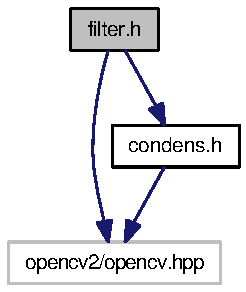
\includegraphics[width=194pt]{filter_8h__incl}
\end{center}
\end{figure}
This graph shows which files directly or indirectly include this file\-:\nopagebreak
\begin{figure}[H]
\begin{center}
\leavevmode
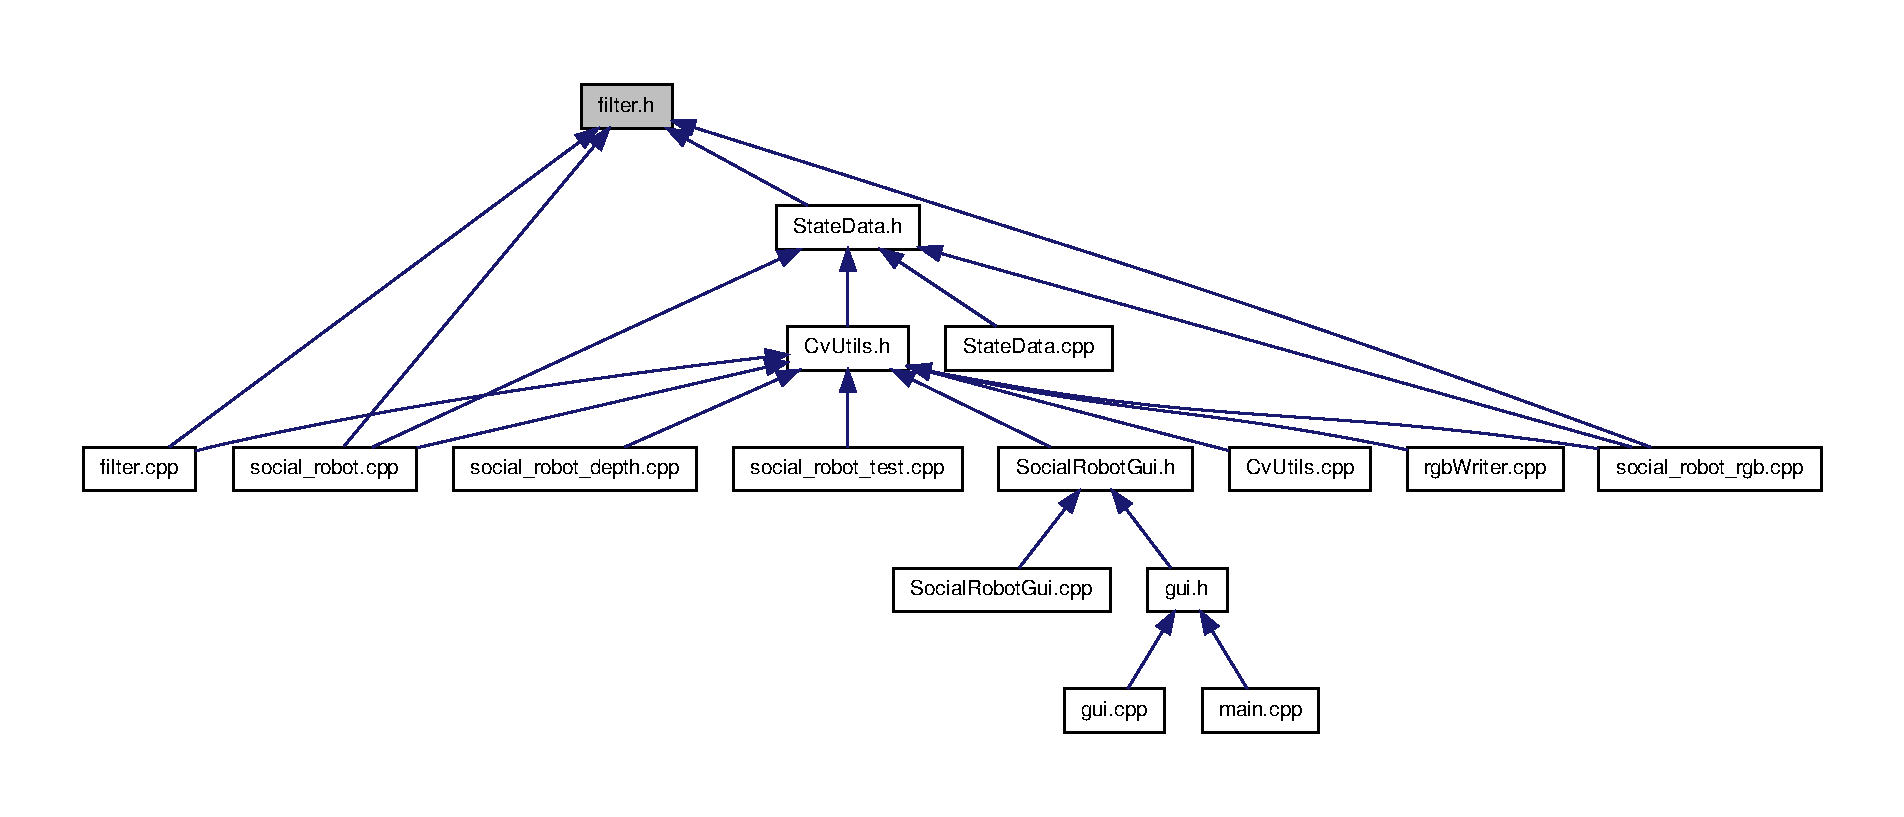
\includegraphics[width=292pt]{filter_8h__dep__incl}
\end{center}
\end{figure}
\subsection*{Data Structures}
\begin{DoxyCompactItemize}
\item 
class \hyperlink{classParticleFilter}{Particle\-Filter}
\end{DoxyCompactItemize}

\hypertarget{gui_8cpp}{\section{gui.\-cpp File Reference}
\label{gui_8cpp}\index{gui.\-cpp@{gui.\-cpp}}
}
{\ttfamily \#include \char`\"{}gui.\-h\char`\"{}}\\*
{\ttfamily \#include $<$Q\-String\-List$>$}\\*
{\ttfamily \#include $<$Q\-File\-Dialog$>$}\\*
{\ttfamily \#include $<$Q\-Debug$>$}\\*
{\ttfamily \#include $<$Q\-Message\-Box$>$}\\*
{\ttfamily \#include $<$string$>$}\\*
{\ttfamily \#include \char`\"{}imageframe.\-h\char`\"{}}\\*
Include dependency graph for gui.\-cpp\-:
\nopagebreak
\begin{figure}[H]
\begin{center}
\leavevmode
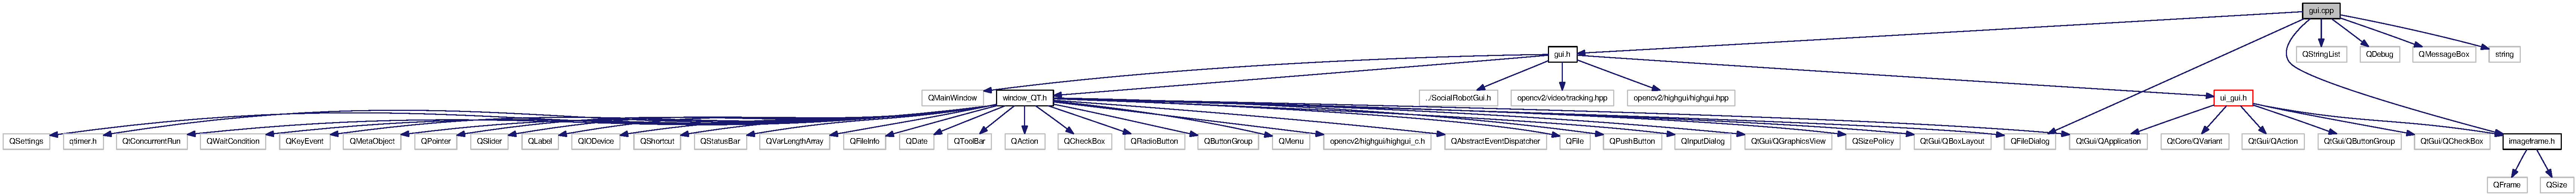
\includegraphics[width=350pt]{gui_8cpp__incl}
\end{center}
\end{figure}

\hypertarget{gui_8h}{\section{gui.\-h File Reference}
\label{gui_8h}\index{gui.\-h@{gui.\-h}}
}
{\ttfamily \#include $<$Q\-Main\-Window$>$}\\*
{\ttfamily \#include $<$opencv2/video/tracking.\-hpp$>$}\\*
{\ttfamily \#include $<$opencv2/highgui/highgui.\-hpp$>$}\\*
{\ttfamily \#include \char`\"{}window\-\_\-\-Q\-T.\-h\char`\"{}}\\*
{\ttfamily \#include \char`\"{}ui\-\_\-gui.\-h\char`\"{}}\\*
{\ttfamily \#include \char`\"{}../\-Social\-Robot\-Gui.\-h\char`\"{}}\\*
Include dependency graph for gui.\-h\-:\nopagebreak
\begin{figure}[H]
\begin{center}
\leavevmode
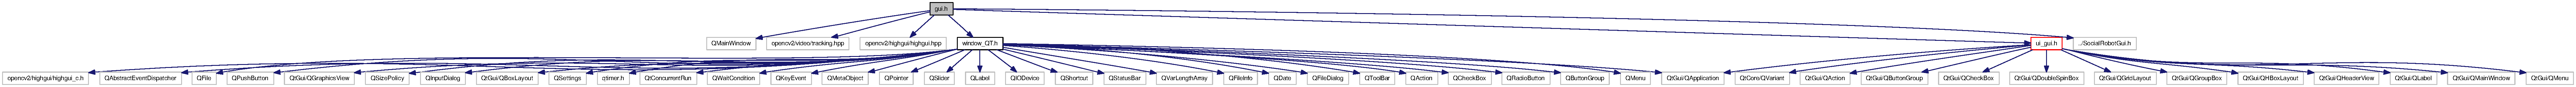
\includegraphics[width=350pt]{gui_8h__incl}
\end{center}
\end{figure}
This graph shows which files directly or indirectly include this file\-:\nopagebreak
\begin{figure}[H]
\begin{center}
\leavevmode
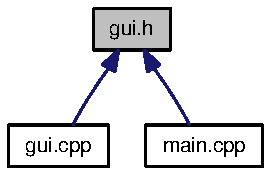
\includegraphics[width=202pt]{gui_8h__dep__incl}
\end{center}
\end{figure}
\subsection*{Data Structures}
\begin{DoxyCompactItemize}
\item 
class \hyperlink{classGui}{Gui}
\end{DoxyCompactItemize}

\hypertarget{hist_8cpp}{
\section{hist.cpp File Reference}
\label{hist_8cpp}\index{hist.cpp@{hist.cpp}}
}
{\ttfamily \#include \char`\"{}hist.h\char`\"{}}\par
Include dependency graph for hist.cpp:\nopagebreak
\begin{figure}[H]
\begin{center}
\leavevmode
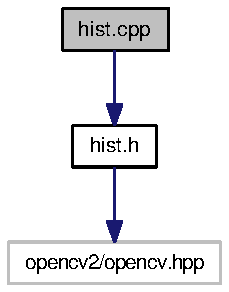
\includegraphics[width=73pt]{hist_8cpp__incl}
\end{center}
\end{figure}
\subsection*{Functions}
\begin{DoxyCompactItemize}
\item 
void \hyperlink{hist_8cpp_a1a38b112a03ec37742029c6d118dfd31}{calc\_\-hist\_\-bgrd} (Mat \&bgr, Mat \&depth, Mat \&hist)
\item 
void \hyperlink{hist_8cpp_a65d5cc321bb3bd97b2e5783f5e67cd87}{calc\_\-hist\_\-d} (Mat \&depth, Mat \&hist)
\item 
void \hyperlink{hist_8cpp_a85106f1dbe0df1c45ea8559ef060ad3c}{calc\_\-hist\_\-bgr} (Mat \&bgr, Mat \&hist)
\item 
void \hyperlink{hist_8cpp_adbbb6b1f2d4ead4bdb1fb22ff5bb0096}{calc\_\-hist} (Mat \&bgr, Mat \&depth, Mat \&hist, int type)
\end{DoxyCompactItemize}


\subsection{Function Documentation}
\hypertarget{hist_8cpp_adbbb6b1f2d4ead4bdb1fb22ff5bb0096}{
\index{hist.cpp@{hist.cpp}!calc\_\-hist@{calc\_\-hist}}
\index{calc\_\-hist@{calc\_\-hist}!hist.cpp@{hist.cpp}}
\subsubsection[{calc\_\-hist}]{\setlength{\rightskip}{0pt plus 5cm}void calc\_\-hist (Mat \& {\em bgr}, \/  Mat \& {\em depth}, \/  Mat \& {\em hist}, \/  int {\em type})}}
\label{hist_8cpp_adbbb6b1f2d4ead4bdb1fb22ff5bb0096}
\hypertarget{hist_8cpp_a85106f1dbe0df1c45ea8559ef060ad3c}{
\index{hist.cpp@{hist.cpp}!calc\_\-hist\_\-bgr@{calc\_\-hist\_\-bgr}}
\index{calc\_\-hist\_\-bgr@{calc\_\-hist\_\-bgr}!hist.cpp@{hist.cpp}}
\subsubsection[{calc\_\-hist\_\-bgr}]{\setlength{\rightskip}{0pt plus 5cm}void calc\_\-hist\_\-bgr (Mat \& {\em bgr}, \/  Mat \& {\em hist})\hspace{0.3cm}{\ttfamily  \mbox{[}inline\mbox{]}}}}
\label{hist_8cpp_a85106f1dbe0df1c45ea8559ef060ad3c}
\hypertarget{hist_8cpp_a1a38b112a03ec37742029c6d118dfd31}{
\index{hist.cpp@{hist.cpp}!calc\_\-hist\_\-bgrd@{calc\_\-hist\_\-bgrd}}
\index{calc\_\-hist\_\-bgrd@{calc\_\-hist\_\-bgrd}!hist.cpp@{hist.cpp}}
\subsubsection[{calc\_\-hist\_\-bgrd}]{\setlength{\rightskip}{0pt plus 5cm}void calc\_\-hist\_\-bgrd (Mat \& {\em bgr}, \/  Mat \& {\em depth}, \/  Mat \& {\em hist})\hspace{0.3cm}{\ttfamily  \mbox{[}inline\mbox{]}}}}
\label{hist_8cpp_a1a38b112a03ec37742029c6d118dfd31}
\hypertarget{hist_8cpp_a65d5cc321bb3bd97b2e5783f5e67cd87}{
\index{hist.cpp@{hist.cpp}!calc\_\-hist\_\-d@{calc\_\-hist\_\-d}}
\index{calc\_\-hist\_\-d@{calc\_\-hist\_\-d}!hist.cpp@{hist.cpp}}
\subsubsection[{calc\_\-hist\_\-d}]{\setlength{\rightskip}{0pt plus 5cm}void calc\_\-hist\_\-d (Mat \& {\em depth}, \/  Mat \& {\em hist})\hspace{0.3cm}{\ttfamily  \mbox{[}inline\mbox{]}}}}
\label{hist_8cpp_a65d5cc321bb3bd97b2e5783f5e67cd87}

\hypertarget{hist_8h}{\section{hist.\-h File Reference}
\label{hist_8h}\index{hist.\-h@{hist.\-h}}
}
{\ttfamily \#include $<$opencv2/opencv.\-hpp$>$}\\*
Include dependency graph for hist.\-h\-:
\nopagebreak
\begin{figure}[H]
\begin{center}
\leavevmode
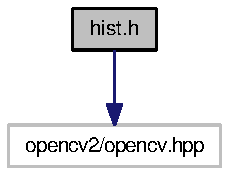
\includegraphics[width=186pt]{hist_8h__incl}
\end{center}
\end{figure}
This graph shows which files directly or indirectly include this file\-:
\nopagebreak
\begin{figure}[H]
\begin{center}
\leavevmode
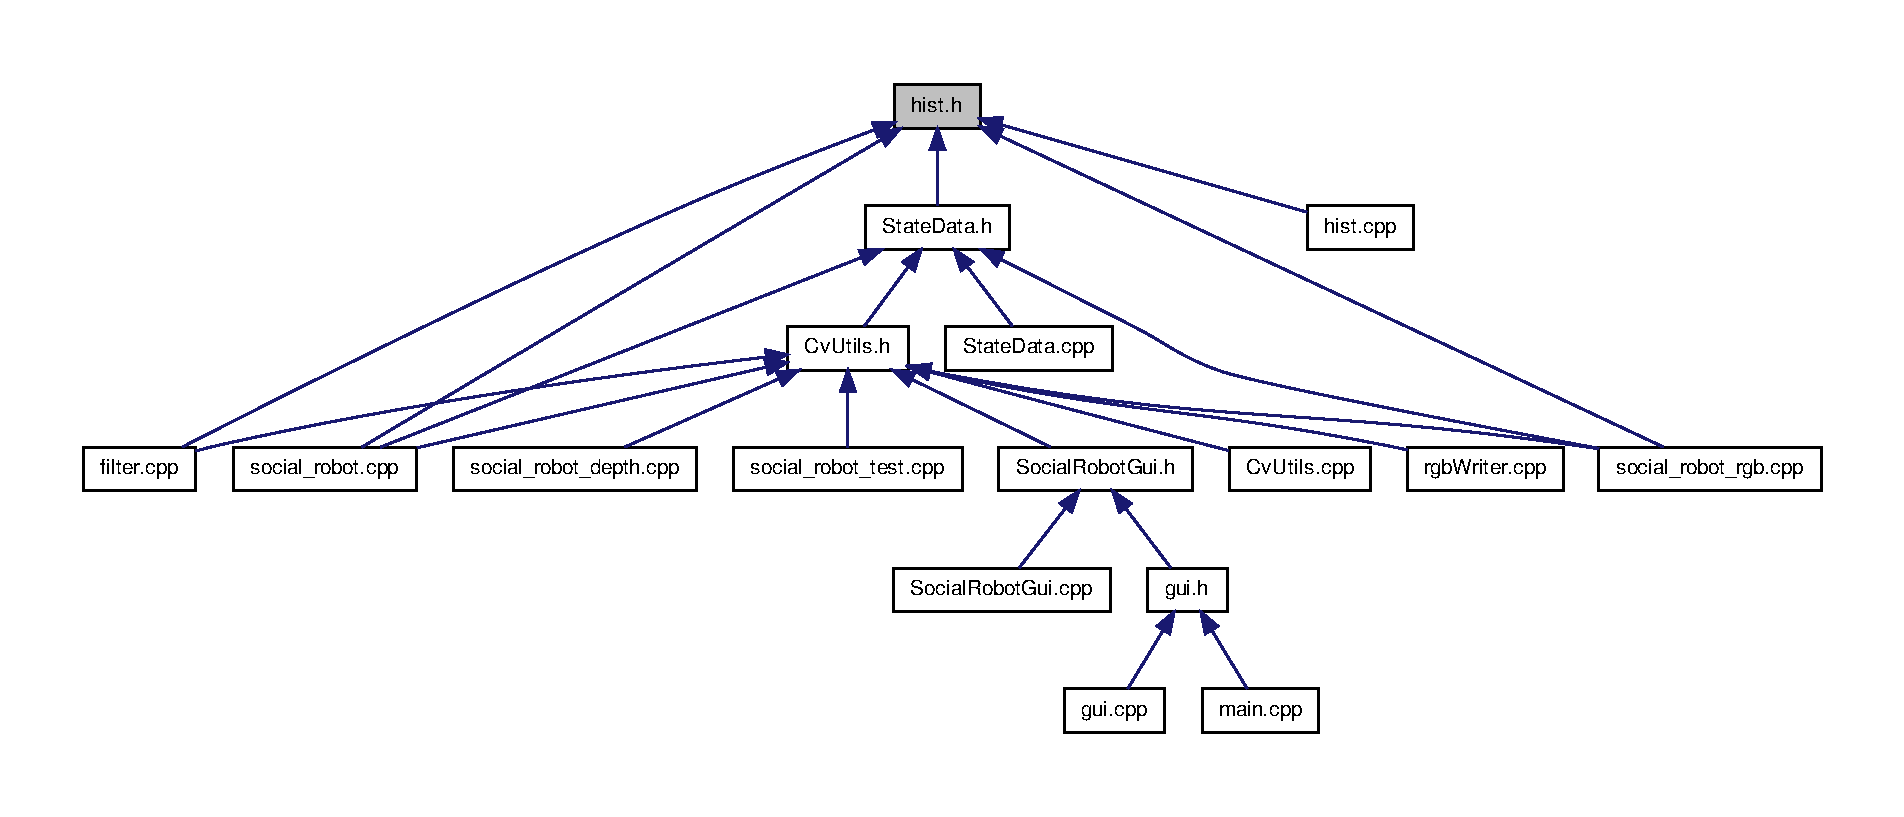
\includegraphics[width=350pt]{hist_8h__dep__incl}
\end{center}
\end{figure}
\subsection*{Functions}
\begin{DoxyCompactItemize}
\item 
void \hyperlink{hist_8h_a14f6a44c7f99a066b24a0b04e9defe89}{calc\-\_\-hist} (cv\-::\-Mat \&bgr, cv\-::\-Mat \&depth, cv\-::\-Mat \&hist, int type)
\end{DoxyCompactItemize}


\subsection{Function Documentation}
\hypertarget{hist_8h_a14f6a44c7f99a066b24a0b04e9defe89}{\index{hist.\-h@{hist.\-h}!calc\-\_\-hist@{calc\-\_\-hist}}
\index{calc\-\_\-hist@{calc\-\_\-hist}!hist.h@{hist.\-h}}
\subsubsection[{calc\-\_\-hist}]{\setlength{\rightskip}{0pt plus 5cm}void calc\-\_\-hist (
\begin{DoxyParamCaption}
\item[{cv\-::\-Mat \&}]{bgr, }
\item[{cv\-::\-Mat \&}]{depth, }
\item[{cv\-::\-Mat \&}]{hist, }
\item[{int}]{type}
\end{DoxyParamCaption}
)}}\label{hist_8h_a14f6a44c7f99a066b24a0b04e9defe89}
\begin{DoxyCopyright}{Copyright}

\end{DoxyCopyright}
Copyright 2012 Kevin Schluff

This program is free software\-: you can redistribute it and/or modify it under the terms of the G\-N\-U General Public License version 2, as published by the Free Software Foundation.

This program is distributed in the hope that it will be useful, but W\-I\-T\-H\-O\-U\-T A\-N\-Y W\-A\-R\-R\-A\-N\-T\-Y; without even the implied warranty of M\-E\-R\-C\-H\-A\-N\-T\-A\-B\-I\-L\-I\-T\-Y or F\-I\-T\-N\-E\-S\-S F\-O\-R A P\-A\-R\-T\-I\-C\-U\-L\-A\-R P\-U\-R\-P\-O\-S\-E. See the G\-N\-U General Public License for more details.

You should have received a copy of the G\-N\-U General Public License along with this program. If not, see \href{http://www.gnu.org/licenses/}{\tt http\-://www.\-gnu.\-org/licenses/}. 
\hypertarget{imageframe_8cpp}{
\section{imageframe.cpp File Reference}
\label{imageframe_8cpp}\index{imageframe.cpp@{imageframe.cpp}}
}
{\ttfamily \#include \char`\"{}imageframe.h\char`\"{}}\par
{\ttfamily \#include $<$QResizeEvent$>$}\par
Include dependency graph for imageframe.cpp:\nopagebreak
\begin{figure}[H]
\begin{center}
\leavevmode
\includegraphics[width=117pt]{imageframe_8cpp__incl}
\end{center}
\end{figure}

\hypertarget{imageframe_8h}{\section{imageframe.\-h File Reference}
\label{imageframe_8h}\index{imageframe.\-h@{imageframe.\-h}}
}
{\ttfamily \#include $<$Q\-Frame$>$}\\*
{\ttfamily \#include $<$Q\-Size$>$}\\*
Include dependency graph for imageframe.\-h\-:\nopagebreak
\begin{figure}[H]
\begin{center}
\leavevmode
\includegraphics[width=194pt]{imageframe_8h__incl}
\end{center}
\end{figure}
This graph shows which files directly or indirectly include this file\-:\nopagebreak
\begin{figure}[H]
\begin{center}
\leavevmode
\includegraphics[width=232pt]{imageframe_8h__dep__incl}
\end{center}
\end{figure}
\subsection*{Data Structures}
\begin{DoxyCompactItemize}
\item 
class \hyperlink{classImageFrame}{Image\-Frame}
\end{DoxyCompactItemize}

\hypertarget{kinect__proxy_8cpp}{\section{kinect\-\_\-proxy.\-cpp File Reference}
\label{kinect__proxy_8cpp}\index{kinect\-\_\-proxy.\-cpp@{kinect\-\_\-proxy.\-cpp}}
}
{\ttfamily \#include \char`\"{}kinect\-\_\-proxy.\-h\char`\"{}}\\*
{\ttfamily \#include $<$std\-\_\-srvs/\-Empty.\-h$>$}\\*
{\ttfamily \#include $<$stereo\-\_\-msgs/\-Disparity\-Image.\-h$>$}\\*
Include dependency graph for kinect\-\_\-proxy.\-cpp\-:
\nopagebreak
\begin{figure}[H]
\begin{center}
\leavevmode
\includegraphics[width=350pt]{kinect__proxy_8cpp__incl}
\end{center}
\end{figure}
\subsection*{Functions}
\begin{DoxyCompactItemize}
\item 
bool \hyperlink{kinect__proxy_8cpp_a9ae57c8616e667d87eb886fabacc1558}{save\-\_\-all} (std\-\_\-srvs\-::\-Empty\-::\-Request \&, std\-\_\-srvs\-::\-Empty\-::\-Response \&)
\item 
bool \hyperlink{kinect__proxy_8cpp_a0e8a83ce1a9ac4b71609a8b3888fa52e}{save\-\_\-depth} (std\-\_\-srvs\-::\-Empty\-::\-Request \&, std\-\_\-srvs\-::\-Empty\-::\-Response \&)
\item 
bool \hyperlink{kinect__proxy_8cpp_a090bbb3c5d76fadb440d9a20bdd89711}{save\-\_\-rgb} (std\-\_\-srvs\-::\-Empty\-::\-Request \&, std\-\_\-srvs\-::\-Empty\-::\-Response \&)
\item 
bool \hyperlink{kinect__proxy_8cpp_a44369042abd96f9024b35acbb673c272}{save\-\_\-disparity} (std\-\_\-srvs\-::\-Empty\-::\-Request \&, std\-\_\-srvs\-::\-Empty\-::\-Response \&)
\item 
bool \hyperlink{kinect__proxy_8cpp_a9a4ea1ed390aea879b048dd9953b90df}{save\-\_\-ir} (std\-\_\-srvs\-::\-Empty\-::\-Request \&, std\-\_\-srvs\-::\-Empty\-::\-Response \&)
\item 
void \hyperlink{kinect__proxy_8cpp_a8822e21670e8549d4c51bad4c96890d9}{rgb\-\_\-cb} (const sensor\-\_\-msgs\-::\-Image\-Const\-Ptr \&msg)
\item 
void \hyperlink{kinect__proxy_8cpp_aa59cb262fc28be47854d4ce4314ccbe1}{depth\-\_\-cb} (const sensor\-\_\-msgs\-::\-Image\-Const\-Ptr \&msg)
\item 
void \hyperlink{kinect__proxy_8cpp_a0d3fad22151b4866ff40824b1f16610c}{disparity\-\_\-cb} (const stereo\-\_\-msgs\-::\-Disparity\-Image\-Const\-Ptr \&msg)
\item 
void \hyperlink{kinect__proxy_8cpp_a10eead4448e002f15c22164d23e2744c}{ir\-\_\-cb} (const sensor\-\_\-msgs\-::\-Image\-Const\-Ptr \&msg)
\item 
void \hyperlink{kinect__proxy_8cpp_a2fbba66df0f87e05ea50652ba86376a1}{init\-\_\-kinect} (void)
\end{DoxyCompactItemize}
\subsection*{Variables}
\begin{DoxyCompactItemize}
\item 
cv\-\_\-bridge\-::\-Cv\-Image\-Ptr \hyperlink{kinect__proxy_8cpp_a5df8b6f1edb3949553518acb419629e5}{cv\-\_\-rgb}
\item 
cv\-\_\-bridge\-::\-Cv\-Image\-Ptr \hyperlink{kinect__proxy_8cpp_a12179be667cc00598b34397d4591f4d7}{cv\-\_\-depth}
\item 
cv\-\_\-bridge\-::\-Cv\-Image\-Ptr \hyperlink{kinect__proxy_8cpp_a25c3fe76b7fae57b1989dc80ceee2070}{cv\-\_\-disparity}
\item 
cv\-\_\-bridge\-::\-Cv\-Image\-Ptr \hyperlink{kinect__proxy_8cpp_a749b79c9dbed1006896a465bd08ca4a1}{cv\-\_\-ir}
\end{DoxyCompactItemize}


\subsection{Function Documentation}
\hypertarget{kinect__proxy_8cpp_aa59cb262fc28be47854d4ce4314ccbe1}{\index{kinect\-\_\-proxy.\-cpp@{kinect\-\_\-proxy.\-cpp}!depth\-\_\-cb@{depth\-\_\-cb}}
\index{depth\-\_\-cb@{depth\-\_\-cb}!kinect_proxy.cpp@{kinect\-\_\-proxy.\-cpp}}
\subsubsection[{depth\-\_\-cb}]{\setlength{\rightskip}{0pt plus 5cm}void depth\-\_\-cb (
\begin{DoxyParamCaption}
\item[{const sensor\-\_\-msgs\-::\-Image\-Const\-Ptr \&}]{msg}
\end{DoxyParamCaption}
)}}\label{kinect__proxy_8cpp_aa59cb262fc28be47854d4ce4314ccbe1}
\hypertarget{kinect__proxy_8cpp_a0d3fad22151b4866ff40824b1f16610c}{\index{kinect\-\_\-proxy.\-cpp@{kinect\-\_\-proxy.\-cpp}!disparity\-\_\-cb@{disparity\-\_\-cb}}
\index{disparity\-\_\-cb@{disparity\-\_\-cb}!kinect_proxy.cpp@{kinect\-\_\-proxy.\-cpp}}
\subsubsection[{disparity\-\_\-cb}]{\setlength{\rightskip}{0pt plus 5cm}void disparity\-\_\-cb (
\begin{DoxyParamCaption}
\item[{const stereo\-\_\-msgs\-::\-Disparity\-Image\-Const\-Ptr \&}]{msg}
\end{DoxyParamCaption}
)}}\label{kinect__proxy_8cpp_a0d3fad22151b4866ff40824b1f16610c}
\hypertarget{kinect__proxy_8cpp_a2fbba66df0f87e05ea50652ba86376a1}{\index{kinect\-\_\-proxy.\-cpp@{kinect\-\_\-proxy.\-cpp}!init\-\_\-kinect@{init\-\_\-kinect}}
\index{init\-\_\-kinect@{init\-\_\-kinect}!kinect_proxy.cpp@{kinect\-\_\-proxy.\-cpp}}
\subsubsection[{init\-\_\-kinect}]{\setlength{\rightskip}{0pt plus 5cm}void init\-\_\-kinect (
\begin{DoxyParamCaption}
\item[{void}]{}
\end{DoxyParamCaption}
)}}\label{kinect__proxy_8cpp_a2fbba66df0f87e05ea50652ba86376a1}
\hypertarget{kinect__proxy_8cpp_a10eead4448e002f15c22164d23e2744c}{\index{kinect\-\_\-proxy.\-cpp@{kinect\-\_\-proxy.\-cpp}!ir\-\_\-cb@{ir\-\_\-cb}}
\index{ir\-\_\-cb@{ir\-\_\-cb}!kinect_proxy.cpp@{kinect\-\_\-proxy.\-cpp}}
\subsubsection[{ir\-\_\-cb}]{\setlength{\rightskip}{0pt plus 5cm}void ir\-\_\-cb (
\begin{DoxyParamCaption}
\item[{const sensor\-\_\-msgs\-::\-Image\-Const\-Ptr \&}]{msg}
\end{DoxyParamCaption}
)}}\label{kinect__proxy_8cpp_a10eead4448e002f15c22164d23e2744c}
\hypertarget{kinect__proxy_8cpp_a8822e21670e8549d4c51bad4c96890d9}{\index{kinect\-\_\-proxy.\-cpp@{kinect\-\_\-proxy.\-cpp}!rgb\-\_\-cb@{rgb\-\_\-cb}}
\index{rgb\-\_\-cb@{rgb\-\_\-cb}!kinect_proxy.cpp@{kinect\-\_\-proxy.\-cpp}}
\subsubsection[{rgb\-\_\-cb}]{\setlength{\rightskip}{0pt plus 5cm}void rgb\-\_\-cb (
\begin{DoxyParamCaption}
\item[{const sensor\-\_\-msgs\-::\-Image\-Const\-Ptr \&}]{msg}
\end{DoxyParamCaption}
)}}\label{kinect__proxy_8cpp_a8822e21670e8549d4c51bad4c96890d9}
\hypertarget{kinect__proxy_8cpp_a9ae57c8616e667d87eb886fabacc1558}{\index{kinect\-\_\-proxy.\-cpp@{kinect\-\_\-proxy.\-cpp}!save\-\_\-all@{save\-\_\-all}}
\index{save\-\_\-all@{save\-\_\-all}!kinect_proxy.cpp@{kinect\-\_\-proxy.\-cpp}}
\subsubsection[{save\-\_\-all}]{\setlength{\rightskip}{0pt plus 5cm}bool save\-\_\-all (
\begin{DoxyParamCaption}
\item[{std\-\_\-srvs\-::\-Empty\-::\-Request \&}]{, }
\item[{std\-\_\-srvs\-::\-Empty\-::\-Response \&}]{}
\end{DoxyParamCaption}
)}}\label{kinect__proxy_8cpp_a9ae57c8616e667d87eb886fabacc1558}
\hypertarget{kinect__proxy_8cpp_a0e8a83ce1a9ac4b71609a8b3888fa52e}{\index{kinect\-\_\-proxy.\-cpp@{kinect\-\_\-proxy.\-cpp}!save\-\_\-depth@{save\-\_\-depth}}
\index{save\-\_\-depth@{save\-\_\-depth}!kinect_proxy.cpp@{kinect\-\_\-proxy.\-cpp}}
\subsubsection[{save\-\_\-depth}]{\setlength{\rightskip}{0pt plus 5cm}bool save\-\_\-depth (
\begin{DoxyParamCaption}
\item[{std\-\_\-srvs\-::\-Empty\-::\-Request \&}]{, }
\item[{std\-\_\-srvs\-::\-Empty\-::\-Response \&}]{}
\end{DoxyParamCaption}
)}}\label{kinect__proxy_8cpp_a0e8a83ce1a9ac4b71609a8b3888fa52e}
\hypertarget{kinect__proxy_8cpp_a44369042abd96f9024b35acbb673c272}{\index{kinect\-\_\-proxy.\-cpp@{kinect\-\_\-proxy.\-cpp}!save\-\_\-disparity@{save\-\_\-disparity}}
\index{save\-\_\-disparity@{save\-\_\-disparity}!kinect_proxy.cpp@{kinect\-\_\-proxy.\-cpp}}
\subsubsection[{save\-\_\-disparity}]{\setlength{\rightskip}{0pt plus 5cm}bool save\-\_\-disparity (
\begin{DoxyParamCaption}
\item[{std\-\_\-srvs\-::\-Empty\-::\-Request \&}]{, }
\item[{std\-\_\-srvs\-::\-Empty\-::\-Response \&}]{}
\end{DoxyParamCaption}
)}}\label{kinect__proxy_8cpp_a44369042abd96f9024b35acbb673c272}
\hypertarget{kinect__proxy_8cpp_a9a4ea1ed390aea879b048dd9953b90df}{\index{kinect\-\_\-proxy.\-cpp@{kinect\-\_\-proxy.\-cpp}!save\-\_\-ir@{save\-\_\-ir}}
\index{save\-\_\-ir@{save\-\_\-ir}!kinect_proxy.cpp@{kinect\-\_\-proxy.\-cpp}}
\subsubsection[{save\-\_\-ir}]{\setlength{\rightskip}{0pt plus 5cm}bool save\-\_\-ir (
\begin{DoxyParamCaption}
\item[{std\-\_\-srvs\-::\-Empty\-::\-Request \&}]{, }
\item[{std\-\_\-srvs\-::\-Empty\-::\-Response \&}]{}
\end{DoxyParamCaption}
)}}\label{kinect__proxy_8cpp_a9a4ea1ed390aea879b048dd9953b90df}
\hypertarget{kinect__proxy_8cpp_a090bbb3c5d76fadb440d9a20bdd89711}{\index{kinect\-\_\-proxy.\-cpp@{kinect\-\_\-proxy.\-cpp}!save\-\_\-rgb@{save\-\_\-rgb}}
\index{save\-\_\-rgb@{save\-\_\-rgb}!kinect_proxy.cpp@{kinect\-\_\-proxy.\-cpp}}
\subsubsection[{save\-\_\-rgb}]{\setlength{\rightskip}{0pt plus 5cm}bool save\-\_\-rgb (
\begin{DoxyParamCaption}
\item[{std\-\_\-srvs\-::\-Empty\-::\-Request \&}]{, }
\item[{std\-\_\-srvs\-::\-Empty\-::\-Response \&}]{}
\end{DoxyParamCaption}
)}}\label{kinect__proxy_8cpp_a090bbb3c5d76fadb440d9a20bdd89711}


\subsection{Variable Documentation}
\hypertarget{kinect__proxy_8cpp_a12179be667cc00598b34397d4591f4d7}{\index{kinect\-\_\-proxy.\-cpp@{kinect\-\_\-proxy.\-cpp}!cv\-\_\-depth@{cv\-\_\-depth}}
\index{cv\-\_\-depth@{cv\-\_\-depth}!kinect_proxy.cpp@{kinect\-\_\-proxy.\-cpp}}
\subsubsection[{cv\-\_\-depth}]{\setlength{\rightskip}{0pt plus 5cm}cv\-\_\-bridge\-::\-Cv\-Image\-Ptr cv\-\_\-depth}}\label{kinect__proxy_8cpp_a12179be667cc00598b34397d4591f4d7}
\hypertarget{kinect__proxy_8cpp_a25c3fe76b7fae57b1989dc80ceee2070}{\index{kinect\-\_\-proxy.\-cpp@{kinect\-\_\-proxy.\-cpp}!cv\-\_\-disparity@{cv\-\_\-disparity}}
\index{cv\-\_\-disparity@{cv\-\_\-disparity}!kinect_proxy.cpp@{kinect\-\_\-proxy.\-cpp}}
\subsubsection[{cv\-\_\-disparity}]{\setlength{\rightskip}{0pt plus 5cm}cv\-\_\-bridge\-::\-Cv\-Image\-Ptr cv\-\_\-disparity}}\label{kinect__proxy_8cpp_a25c3fe76b7fae57b1989dc80ceee2070}
\hypertarget{kinect__proxy_8cpp_a749b79c9dbed1006896a465bd08ca4a1}{\index{kinect\-\_\-proxy.\-cpp@{kinect\-\_\-proxy.\-cpp}!cv\-\_\-ir@{cv\-\_\-ir}}
\index{cv\-\_\-ir@{cv\-\_\-ir}!kinect_proxy.cpp@{kinect\-\_\-proxy.\-cpp}}
\subsubsection[{cv\-\_\-ir}]{\setlength{\rightskip}{0pt plus 5cm}cv\-\_\-bridge\-::\-Cv\-Image\-Ptr cv\-\_\-ir}}\label{kinect__proxy_8cpp_a749b79c9dbed1006896a465bd08ca4a1}
\hypertarget{kinect__proxy_8cpp_a5df8b6f1edb3949553518acb419629e5}{\index{kinect\-\_\-proxy.\-cpp@{kinect\-\_\-proxy.\-cpp}!cv\-\_\-rgb@{cv\-\_\-rgb}}
\index{cv\-\_\-rgb@{cv\-\_\-rgb}!kinect_proxy.cpp@{kinect\-\_\-proxy.\-cpp}}
\subsubsection[{cv\-\_\-rgb}]{\setlength{\rightskip}{0pt plus 5cm}cv\-\_\-bridge\-::\-Cv\-Image\-Ptr cv\-\_\-rgb}}\label{kinect__proxy_8cpp_a5df8b6f1edb3949553518acb419629e5}

\hypertarget{kinect__proxy_8h}{\section{kinect\-\_\-proxy.\-h File Reference}
\label{kinect__proxy_8h}\index{kinect\-\_\-proxy.\-h@{kinect\-\_\-proxy.\-h}}
}
{\ttfamily \#include $<$ros/ros.\-h$>$}\\*
{\ttfamily \#include $<$ros/package.\-h$>$}\\*
{\ttfamily \#include $<$image\-\_\-transport/image\-\_\-transport.\-h$>$}\\*
{\ttfamily \#include $<$cv\-\_\-bridge/cv\-\_\-bridge.\-h$>$}\\*
{\ttfamily \#include $<$sensor\-\_\-msgs/image\-\_\-encodings.\-h$>$}\\*
{\ttfamily \#include $<$opencv2/core/core.\-hpp$>$}\\*
{\ttfamily \#include $<$opencv2/imgproc/imgproc.\-hpp$>$}\\*
{\ttfamily \#include $<$opencv2/highgui/highgui.\-hpp$>$}\\*
{\ttfamily \#include \char`\"{}string\-\_\-utils.\-h\char`\"{}}\\*
Include dependency graph for kinect\-\_\-proxy.\-h\-:
\nopagebreak
\begin{figure}[H]
\begin{center}
\leavevmode
\includegraphics[width=350pt]{kinect__proxy_8h__incl}
\end{center}
\end{figure}
This graph shows which files directly or indirectly include this file\-:
\nopagebreak
\begin{figure}[H]
\begin{center}
\leavevmode
\includegraphics[width=350pt]{kinect__proxy_8h__dep__incl}
\end{center}
\end{figure}
\subsection*{Functions}
\begin{DoxyCompactItemize}
\item 
void \hyperlink{kinect__proxy_8h_a2fbba66df0f87e05ea50652ba86376a1}{init\-\_\-kinect} (void)
\end{DoxyCompactItemize}


\subsection{Function Documentation}
\hypertarget{kinect__proxy_8h_a2fbba66df0f87e05ea50652ba86376a1}{\index{kinect\-\_\-proxy.\-h@{kinect\-\_\-proxy.\-h}!init\-\_\-kinect@{init\-\_\-kinect}}
\index{init\-\_\-kinect@{init\-\_\-kinect}!kinect_proxy.h@{kinect\-\_\-proxy.\-h}}
\subsubsection[{init\-\_\-kinect}]{\setlength{\rightskip}{0pt plus 5cm}void init\-\_\-kinect (
\begin{DoxyParamCaption}
\item[{void}]{}
\end{DoxyParamCaption}
)}}\label{kinect__proxy_8h_a2fbba66df0f87e05ea50652ba86376a1}

\hypertarget{kinect__save__image_8cpp}{\section{kinect\-\_\-save\-\_\-image.\-cpp File Reference}
\label{kinect__save__image_8cpp}\index{kinect\-\_\-save\-\_\-image.\-cpp@{kinect\-\_\-save\-\_\-image.\-cpp}}
}
{\ttfamily \#include $<$ros/ros.\-h$>$}\\*
{\ttfamily \#include \char`\"{}kinect\-\_\-proxy.\-h\char`\"{}}\\*
Include dependency graph for kinect\-\_\-save\-\_\-image.\-cpp\-:\nopagebreak
\begin{figure}[H]
\begin{center}
\leavevmode
\includegraphics[width=350pt]{kinect__save__image_8cpp__incl}
\end{center}
\end{figure}
\subsection*{Functions}
\begin{DoxyCompactItemize}
\item 
int \hyperlink{kinect__save__image_8cpp_a3c04138a5bfe5d72780bb7e82a18e627}{main} (int argc, char $\ast$$\ast$argv)
\end{DoxyCompactItemize}


\subsection{Function Documentation}
\hypertarget{kinect__save__image_8cpp_a3c04138a5bfe5d72780bb7e82a18e627}{\index{kinect\-\_\-save\-\_\-image.\-cpp@{kinect\-\_\-save\-\_\-image.\-cpp}!main@{main}}
\index{main@{main}!kinect_save_image.cpp@{kinect\-\_\-save\-\_\-image.\-cpp}}
\subsubsection[{main}]{\setlength{\rightskip}{0pt plus 5cm}int main (
\begin{DoxyParamCaption}
\item[{int}]{argc, }
\item[{char $\ast$$\ast$}]{argv}
\end{DoxyParamCaption}
)}}\label{kinect__save__image_8cpp_a3c04138a5bfe5d72780bb7e82a18e627}

\hypertarget{main_8cpp}{\section{main.\-cpp File Reference}
\label{main_8cpp}\index{main.\-cpp@{main.\-cpp}}
}
{\ttfamily \#include $<$Qt\-Gui/\-Q\-Application$>$}\\*
{\ttfamily \#include \char`\"{}gui.\-h\char`\"{}}\\*
Include dependency graph for main.\-cpp\-:\nopagebreak
\begin{figure}[H]
\begin{center}
\leavevmode
\includegraphics[width=350pt]{main_8cpp__incl}
\end{center}
\end{figure}
\subsection*{Functions}
\begin{DoxyCompactItemize}
\item 
int \hyperlink{main_8cpp_a0ddf1224851353fc92bfbff6f499fa97}{main} (int argc, char $\ast$argv\mbox{[}$\,$\mbox{]})
\end{DoxyCompactItemize}


\subsection{Function Documentation}
\hypertarget{main_8cpp_a0ddf1224851353fc92bfbff6f499fa97}{\index{main.\-cpp@{main.\-cpp}!main@{main}}
\index{main@{main}!main.cpp@{main.\-cpp}}
\subsubsection[{main}]{\setlength{\rightskip}{0pt plus 5cm}int main (
\begin{DoxyParamCaption}
\item[{int}]{argc, }
\item[{char $\ast$}]{argv\mbox{[}$\,$\mbox{]}}
\end{DoxyParamCaption}
)}}\label{main_8cpp_a0ddf1224851353fc92bfbff6f499fa97}

\hypertarget{mainpage_8h}{
\section{mainpage.h File Reference}
\label{mainpage_8h}\index{mainpage.h@{mainpage.h}}
}

\hypertarget{PixelSimilarity_8cpp}{\section{Pixel\-Similarity.\-cpp File Reference}
\label{PixelSimilarity_8cpp}\index{Pixel\-Similarity.\-cpp@{Pixel\-Similarity.\-cpp}}
}
{\ttfamily \#include \char`\"{}Pixel\-Similarity.\-h\char`\"{}}\\*
Include dependency graph for Pixel\-Similarity.\-cpp\-:
\nopagebreak
\begin{figure}[H]
\begin{center}
\leavevmode
\includegraphics[width=196pt]{PixelSimilarity_8cpp__incl}
\end{center}
\end{figure}

\hypertarget{PixelSimilarity_8h}{\section{Pixel\-Similarity.\-h File Reference}
\label{PixelSimilarity_8h}\index{Pixel\-Similarity.\-h@{Pixel\-Similarity.\-h}}
}
{\ttfamily \#include $<$opencv2/core/core.\-hpp$>$}\\*
Include dependency graph for Pixel\-Similarity.\-h\-:\nopagebreak
\begin{figure}[H]
\begin{center}
\leavevmode
\includegraphics[width=196pt]{PixelSimilarity_8h__incl}
\end{center}
\end{figure}
This graph shows which files directly or indirectly include this file\-:\nopagebreak
\begin{figure}[H]
\begin{center}
\leavevmode
\includegraphics[width=350pt]{PixelSimilarity_8h__dep__incl}
\end{center}
\end{figure}
\subsection*{Data Structures}
\begin{DoxyCompactItemize}
\item 
class \hyperlink{classPixelSimilarity}{Pixel\-Similarity}
\begin{DoxyCompactList}\small\item\em This class provides the location, radius and likelihood of a given potential head. \end{DoxyCompactList}\end{DoxyCompactItemize}

\hypertarget{rgbWriter_8cpp}{\section{rgb\-Writer.\-cpp File Reference}
\label{rgbWriter_8cpp}\index{rgb\-Writer.\-cpp@{rgb\-Writer.\-cpp}}
}
{\ttfamily \#include $<$ros/ros.\-h$>$}\\*
{\ttfamily \#include $<$std\-\_\-srvs/\-Empty.\-h$>$}\\*
{\ttfamily \#include \char`\"{}../kinect\-\_\-proxy.\-h\char`\"{}}\\*
{\ttfamily \#include \char`\"{}../\-Cv\-Utils.\-h\char`\"{}}\\*
{\ttfamily \#include \char`\"{}../\-Ros\-Utils.\-h\char`\"{}}\\*
Include dependency graph for rgb\-Writer.\-cpp\-:
\nopagebreak
\begin{figure}[H]
\begin{center}
\leavevmode
\includegraphics[width=350pt]{rgbWriter_8cpp__incl}
\end{center}
\end{figure}
\subsection*{Functions}
\begin{DoxyCompactItemize}
\item 
void \hyperlink{rgbWriter_8cpp_a470b337493deec335e4849fd2458dff5}{rgb\-\_\-cb} (const Image\-Const\-Ptr \&msg)
\item 
int \hyperlink{rgbWriter_8cpp_a3c04138a5bfe5d72780bb7e82a18e627}{main} (int argc, char $\ast$$\ast$argv)
\end{DoxyCompactItemize}
\subsection*{Variables}
\begin{DoxyCompactItemize}
\item 
Video\-Writer \hyperlink{rgbWriter_8cpp_a4cc622abec13285a568b13b7b1002d69}{rgbwriter}
\item 
\hyperlink{classCvUtils}{Cv\-Utils} \hyperlink{rgbWriter_8cpp_a199b98558819a161d93892eb6d1f766d}{cv\-\_\-utils}
\item 
bool \hyperlink{rgbWriter_8cpp_a3485ecdd943396c8ba78cc89ef1a4067}{isfirstframe} = true
\end{DoxyCompactItemize}


\subsection{Function Documentation}
\hypertarget{rgbWriter_8cpp_a3c04138a5bfe5d72780bb7e82a18e627}{\index{rgb\-Writer.\-cpp@{rgb\-Writer.\-cpp}!main@{main}}
\index{main@{main}!rgbWriter.cpp@{rgb\-Writer.\-cpp}}
\subsubsection[{main}]{\setlength{\rightskip}{0pt plus 5cm}int main (
\begin{DoxyParamCaption}
\item[{int}]{argc, }
\item[{char $\ast$$\ast$}]{argv}
\end{DoxyParamCaption}
)}}\label{rgbWriter_8cpp_a3c04138a5bfe5d72780bb7e82a18e627}
\hypertarget{rgbWriter_8cpp_a470b337493deec335e4849fd2458dff5}{\index{rgb\-Writer.\-cpp@{rgb\-Writer.\-cpp}!rgb\-\_\-cb@{rgb\-\_\-cb}}
\index{rgb\-\_\-cb@{rgb\-\_\-cb}!rgbWriter.cpp@{rgb\-Writer.\-cpp}}
\subsubsection[{rgb\-\_\-cb}]{\setlength{\rightskip}{0pt plus 5cm}void rgb\-\_\-cb (
\begin{DoxyParamCaption}
\item[{const Image\-Const\-Ptr \&}]{msg}
\end{DoxyParamCaption}
)}}\label{rgbWriter_8cpp_a470b337493deec335e4849fd2458dff5}


\subsection{Variable Documentation}
\hypertarget{rgbWriter_8cpp_a199b98558819a161d93892eb6d1f766d}{\index{rgb\-Writer.\-cpp@{rgb\-Writer.\-cpp}!cv\-\_\-utils@{cv\-\_\-utils}}
\index{cv\-\_\-utils@{cv\-\_\-utils}!rgbWriter.cpp@{rgb\-Writer.\-cpp}}
\subsubsection[{cv\-\_\-utils}]{\setlength{\rightskip}{0pt plus 5cm}{\bf Cv\-Utils} cv\-\_\-utils}}\label{rgbWriter_8cpp_a199b98558819a161d93892eb6d1f766d}
\hypertarget{rgbWriter_8cpp_a3485ecdd943396c8ba78cc89ef1a4067}{\index{rgb\-Writer.\-cpp@{rgb\-Writer.\-cpp}!isfirstframe@{isfirstframe}}
\index{isfirstframe@{isfirstframe}!rgbWriter.cpp@{rgb\-Writer.\-cpp}}
\subsubsection[{isfirstframe}]{\setlength{\rightskip}{0pt plus 5cm}bool isfirstframe = true}}\label{rgbWriter_8cpp_a3485ecdd943396c8ba78cc89ef1a4067}
\hypertarget{rgbWriter_8cpp_a4cc622abec13285a568b13b7b1002d69}{\index{rgb\-Writer.\-cpp@{rgb\-Writer.\-cpp}!rgbwriter@{rgbwriter}}
\index{rgbwriter@{rgbwriter}!rgbWriter.cpp@{rgb\-Writer.\-cpp}}
\subsubsection[{rgbwriter}]{\setlength{\rightskip}{0pt plus 5cm}Video\-Writer rgbwriter}}\label{rgbWriter_8cpp_a4cc622abec13285a568b13b7b1002d69}

\hypertarget{RosUtils_8cpp}{\section{Ros\-Utils.\-cpp File Reference}
\label{RosUtils_8cpp}\index{Ros\-Utils.\-cpp@{Ros\-Utils.\-cpp}}
}
{\ttfamily \#include \char`\"{}Ros\-Utils.\-h\char`\"{}}\\*
Include dependency graph for Ros\-Utils.\-cpp\-:
\nopagebreak
\begin{figure}[H]
\begin{center}
\leavevmode
\includegraphics[width=350pt]{RosUtils_8cpp__incl}
\end{center}
\end{figure}

\hypertarget{RosUtils_8h}{
\section{RosUtils.h File Reference}
\label{RosUtils_8h}\index{RosUtils.h@{RosUtils.h}}
}
{\ttfamily \#include $<$sensor\_\-msgs/RegionOfInterest.h$>$}\par
{\ttfamily \#include $<$opencv2/core/core.hpp$>$}\par
Include dependency graph for RosUtils.h:\nopagebreak
\begin{figure}[H]
\begin{center}
\leavevmode
\includegraphics[width=167pt]{RosUtils_8h__incl}
\end{center}
\end{figure}
This graph shows which files directly or indirectly include this file:\nopagebreak
\begin{figure}[H]
\begin{center}
\leavevmode
\includegraphics[width=341pt]{RosUtils_8h__dep__incl}
\end{center}
\end{figure}
\subsection*{Data Structures}
\begin{DoxyCompactItemize}
\item 
class \hyperlink{classRosUtils}{RosUtils}
\begin{DoxyCompactList}\small\item\em This class is used for publishing the ouput rectangles in ROS. \item\end{DoxyCompactList}\end{DoxyCompactItemize}

\hypertarget{social__robot_8cpp}{\section{social\-\_\-robot.\-cpp File Reference}
\label{social__robot_8cpp}\index{social\-\_\-robot.\-cpp@{social\-\_\-robot.\-cpp}}
}
{\ttfamily \#include $<$ros/ros.\-h$>$}\\*
{\ttfamily \#include $<$std\-\_\-srvs/\-Empty.\-h$>$}\\*
{\ttfamily \#include $<$stereo\-\_\-msgs/\-Disparity\-Image.\-h$>$}\\*
{\ttfamily \#include $<$social\-\_\-robot/\-Region\-Of\-Interests.\-h$>$}\\*
{\ttfamily \#include $<$omp.\-h$>$}\\*
{\ttfamily \#include \char`\"{}kinect\-\_\-proxy.\-h\char`\"{}}\\*
{\ttfamily \#include \char`\"{}Cv\-Utils.\-h\char`\"{}}\\*
{\ttfamily \#include \char`\"{}Ros\-Utils.\-h\char`\"{}}\\*
{\ttfamily \#include \char`\"{}social\-\_\-robot\-\_\-constants.\-h\char`\"{}}\\*
{\ttfamily \#include \char`\"{}particle\-\_\-filter/\-State\-Data.\-h\char`\"{}}\\*
{\ttfamily \#include \char`\"{}particle\-\_\-filter/hist.\-h\char`\"{}}\\*
{\ttfamily \#include \char`\"{}particle\-\_\-filter/filter.\-h\char`\"{}}\\*
Include dependency graph for social\-\_\-robot.\-cpp\-:
\nopagebreak
\begin{figure}[H]
\begin{center}
\leavevmode
\includegraphics[width=350pt]{social__robot_8cpp__incl}
\end{center}
\end{figure}
\subsection*{Functions}
\begin{DoxyCompactItemize}
\item 
void \hyperlink{social__robot_8cpp_afdd6adfc3cdd4dd6e094889fd652dc10}{check\-\_\-update\-\_\-rate\-\_\-frequency} (void)
\item 
void \hyperlink{social__robot_8cpp_a76bdb607b5314ad3f38d4258d94a3bd9}{publish\-\_\-data} (void)
\item 
void \hyperlink{social__robot_8cpp_a9b36af0cbb900e97ef510b6f8925b191}{do\-\_\-tracking} (void)
\item 
void \hyperlink{social__robot_8cpp_ae6e6caa2237ca4d4e003c1976e6ccf75}{data\-\_\-association} (vector$<$ Rect $>$ \&faces)
\item 
bool \hyperlink{social__robot_8cpp_afd0c09aff72c2db54711877905bc09a8}{update\-\_\-param\-\_\-cb} (std\-\_\-srvs\-::\-Empty\-::\-Request \&, std\-\_\-srvs\-::\-Empty\-::\-Response \&)
\item 
void \hyperlink{social__robot_8cpp_a555c9c1104d52ad9cf90f36548ecf4c8}{depth\-\_\-cb} (const Image\-Const\-Ptr \&msg)
\item 
void \hyperlink{social__robot_8cpp_a470b337493deec335e4849fd2458dff5}{rgb\-\_\-cb} (const Image\-Const\-Ptr \&msg)
\item 
void \hyperlink{social__robot_8cpp_a0d3fad22151b4866ff40824b1f16610c}{disparity\-\_\-cb} (const stereo\-\_\-msgs\-::\-Disparity\-Image\-Const\-Ptr \&msg)
\item 
void \hyperlink{social__robot_8cpp_af38efb9182aa491f657f4196e3db7373}{rgb\-\_\-rois\-\_\-cb} (const social\-\_\-robot\-::\-Region\-Of\-Interests \&msg)
\item 
void \hyperlink{social__robot_8cpp_afb90f18aefea6d66d61d6294378b9bd4}{depth\-\_\-rois\-\_\-cb} (const social\-\_\-robot\-::\-Region\-Of\-Interests \&msg)
\item 
void \hyperlink{social__robot_8cpp_a2e656ccae5f85fd17f4f3f4b45b39147}{parse\-\_\-command\-\_\-line} (int argc, char $\ast$$\ast$argv)
\item 
int \hyperlink{social__robot_8cpp_a3c04138a5bfe5d72780bb7e82a18e627}{main} (int argc, char $\ast$$\ast$argv)
\end{DoxyCompactItemize}
\subsection*{Variables}
\begin{DoxyCompactItemize}
\item 
\hyperlink{classRosUtils}{Ros\-Utils} \hyperlink{social__robot_8cpp_abd0f83a9c271173baf120f2aed877bd4}{ros\-\_\-utils}
\item 
social\-\_\-robot\-::\-Region\-Of\-Interests \hyperlink{social__robot_8cpp_ab511b280baa1678d602f858cd02d0902}{depth\-\_\-pub\-\_\-rois}
\item 
ros\-::\-Publisher \hyperlink{social__robot_8cpp_a24924661353a04a9c51bb4a6adcd3d8d}{depth\-\_\-pub}
\item 
ros\-::\-Service\-Client \hyperlink{social__robot_8cpp_ab5f4789bf41f6c6a4c30a5b86239e4a0}{rgb\-\_\-update\-\_\-client}
\item 
ros\-::\-Service\-Client \hyperlink{social__robot_8cpp_aca0cddd05d8abaf3c896cd0d3b19e717}{depth\-\_\-update\-\_\-client}
\item 
std\-\_\-srvs\-::\-Empty \hyperlink{social__robot_8cpp_a5d74a9f34aa4fc850b562dc32bff70ec}{empty}
\item 
ros\-::\-Subscriber \hyperlink{social__robot_8cpp_a0afbd8e1c5321450b872238d81694a60}{rgb\-\_\-rois\-\_\-sub}
\item 
ros\-::\-Subscriber \hyperlink{social__robot_8cpp_a3c30dbde0fb6ec35cb3606bb3bfa2b5a}{depth\-\_\-rois\-\_\-sub}
\item 
double \hyperlink{social__robot_8cpp_a0414cc80d7dc66451dc24ec3418596ee}{track\-\_\-thr} = 100
\item 
double \hyperlink{social__robot_8cpp_aff5593806965b8ace6df9bb9eb072d18}{confidence\-\_\-level\-\_\-thr} = 0.\-90
\item 
double \hyperlink{social__robot_8cpp_ad07b4dff43b9b0209ff0191c9ab669dd}{detection\-\_\-confidence\-\_\-thr} = 0.\-90
\item 
int \hyperlink{social__robot_8cpp_acf574bc864f7f0fc111320f1d6c449d5}{num\-\_\-particles} = 200
\item 
int \hyperlink{social__robot_8cpp_ae605fe87b56cf56cad5443641c5a4534}{rgb\-\_\-framenum} = 0
\item 
int \hyperlink{social__robot_8cpp_acd9505e1fd3d333543dcc08504ad53f0}{rgb\-\_\-update\-\_\-rate} = 1
\item 
int \hyperlink{social__robot_8cpp_afde364f1ed23a565df9eb1bd93ea79b1}{depth\-\_\-framenum} = 0
\item 
int \hyperlink{social__robot_8cpp_a9b7268cc06ede6c34111444cdb0a6dd4}{depth\-\_\-update\-\_\-rate} = 1
\item 
int \hyperlink{social__robot_8cpp_ad0d1c24a698f533bb3bebb6237f85381}{high\-\_\-frequency} = 1
\item 
int \hyperlink{social__robot_8cpp_a748eb5a006a4f3525450c58e5d9721df}{low\-\_\-frequency} = 1
\item 
int \hyperlink{social__robot_8cpp_a5654aa26e4467b244f4098f5e110c92f}{external\-\_\-update\-\_\-rate} = \hyperlink{social__robot_8cpp_ad0d1c24a698f533bb3bebb6237f85381}{high\-\_\-frequency}
\item 
string \hyperlink{social__robot_8cpp_aa2a509dd219d369589809bd049d2cab7}{results\-\_\-filename} = \char`\"{}default\-\_\-results\char`\"{}
\item 
Mat \hyperlink{social__robot_8cpp_adcb087e6e2cbf5d438cf6dd931addf2f}{image\-\_\-disparity}
\item 
Mat \hyperlink{social__robot_8cpp_a80005e5815baea49c1aed806e8e5c3ee}{image\-\_\-depth}
\item 
Mat \hyperlink{social__robot_8cpp_aea3f7c95f70e07adffaf65b6bdfd2e25}{image\-\_\-rgb}
\item 
bool \hyperlink{social__robot_8cpp_ad06ed7936b8404ab824f5c8d2fcc3521}{stand\-\_\-alone} = false
\item 
bool \hyperlink{social__robot_8cpp_ad25bb9dd6e0d75433969a6a0fa569b01}{use\-\_\-colour} = false
\item 
bool \hyperlink{social__robot_8cpp_a8295331a5e3348fc6de66ee0205adafd}{use\-\_\-depth} = false
\item 
vector$<$ \hyperlink{classStateData}{State\-Data} $>$ \hyperlink{social__robot_8cpp_a63ba5e41659a1483954bc6564bca605a}{state\-\_\-datas}
\item 
vector$<$ vector$<$ Rect $>$ $>$ \hyperlink{social__robot_8cpp_a246570e7b14b6616ada8593b04836e1d}{results}
\item 
Video\-Writer \hyperlink{social__robot_8cpp_a4cc622abec13285a568b13b7b1002d69}{rgbwriter}
\item 
bool \hyperlink{social__robot_8cpp_a3485ecdd943396c8ba78cc89ef1a4067}{isfirstframe} = true
\item 
string \hyperlink{social__robot_8cpp_a755d42f2e9c635ce2213e0efad62b796}{file\-\_\-name} = \char`\"{}default.\-avi\char`\"{}
\item 
\hyperlink{classCvUtils}{Cv\-Utils} \hyperlink{social__robot_8cpp_a199b98558819a161d93892eb6d1f766d}{cv\-\_\-utils}
\end{DoxyCompactItemize}


\subsection{Function Documentation}
\hypertarget{social__robot_8cpp_afdd6adfc3cdd4dd6e094889fd652dc10}{\index{social\-\_\-robot.\-cpp@{social\-\_\-robot.\-cpp}!check\-\_\-update\-\_\-rate\-\_\-frequency@{check\-\_\-update\-\_\-rate\-\_\-frequency}}
\index{check\-\_\-update\-\_\-rate\-\_\-frequency@{check\-\_\-update\-\_\-rate\-\_\-frequency}!social_robot.cpp@{social\-\_\-robot.\-cpp}}
\subsubsection[{check\-\_\-update\-\_\-rate\-\_\-frequency}]{\setlength{\rightskip}{0pt plus 5cm}void check\-\_\-update\-\_\-rate\-\_\-frequency (
\begin{DoxyParamCaption}
\item[{void}]{}
\end{DoxyParamCaption}
)}}\label{social__robot_8cpp_afdd6adfc3cdd4dd6e094889fd652dc10}
\hypertarget{social__robot_8cpp_ae6e6caa2237ca4d4e003c1976e6ccf75}{\index{social\-\_\-robot.\-cpp@{social\-\_\-robot.\-cpp}!data\-\_\-association@{data\-\_\-association}}
\index{data\-\_\-association@{data\-\_\-association}!social_robot.cpp@{social\-\_\-robot.\-cpp}}
\subsubsection[{data\-\_\-association}]{\setlength{\rightskip}{0pt plus 5cm}void data\-\_\-association (
\begin{DoxyParamCaption}
\item[{vector$<$ Rect $>$ \&}]{faces}
\end{DoxyParamCaption}
)}}\label{social__robot_8cpp_ae6e6caa2237ca4d4e003c1976e6ccf75}
\hypertarget{social__robot_8cpp_a555c9c1104d52ad9cf90f36548ecf4c8}{\index{social\-\_\-robot.\-cpp@{social\-\_\-robot.\-cpp}!depth\-\_\-cb@{depth\-\_\-cb}}
\index{depth\-\_\-cb@{depth\-\_\-cb}!social_robot.cpp@{social\-\_\-robot.\-cpp}}
\subsubsection[{depth\-\_\-cb}]{\setlength{\rightskip}{0pt plus 5cm}void depth\-\_\-cb (
\begin{DoxyParamCaption}
\item[{const Image\-Const\-Ptr \&}]{msg}
\end{DoxyParamCaption}
)}}\label{social__robot_8cpp_a555c9c1104d52ad9cf90f36548ecf4c8}
\hypertarget{social__robot_8cpp_afb90f18aefea6d66d61d6294378b9bd4}{\index{social\-\_\-robot.\-cpp@{social\-\_\-robot.\-cpp}!depth\-\_\-rois\-\_\-cb@{depth\-\_\-rois\-\_\-cb}}
\index{depth\-\_\-rois\-\_\-cb@{depth\-\_\-rois\-\_\-cb}!social_robot.cpp@{social\-\_\-robot.\-cpp}}
\subsubsection[{depth\-\_\-rois\-\_\-cb}]{\setlength{\rightskip}{0pt plus 5cm}void depth\-\_\-rois\-\_\-cb (
\begin{DoxyParamCaption}
\item[{const social\-\_\-robot\-::\-Region\-Of\-Interests \&}]{msg}
\end{DoxyParamCaption}
)}}\label{social__robot_8cpp_afb90f18aefea6d66d61d6294378b9bd4}
\hypertarget{social__robot_8cpp_a0d3fad22151b4866ff40824b1f16610c}{\index{social\-\_\-robot.\-cpp@{social\-\_\-robot.\-cpp}!disparity\-\_\-cb@{disparity\-\_\-cb}}
\index{disparity\-\_\-cb@{disparity\-\_\-cb}!social_robot.cpp@{social\-\_\-robot.\-cpp}}
\subsubsection[{disparity\-\_\-cb}]{\setlength{\rightskip}{0pt plus 5cm}void disparity\-\_\-cb (
\begin{DoxyParamCaption}
\item[{const stereo\-\_\-msgs\-::\-Disparity\-Image\-Const\-Ptr \&}]{msg}
\end{DoxyParamCaption}
)}}\label{social__robot_8cpp_a0d3fad22151b4866ff40824b1f16610c}
\hypertarget{social__robot_8cpp_a9b36af0cbb900e97ef510b6f8925b191}{\index{social\-\_\-robot.\-cpp@{social\-\_\-robot.\-cpp}!do\-\_\-tracking@{do\-\_\-tracking}}
\index{do\-\_\-tracking@{do\-\_\-tracking}!social_robot.cpp@{social\-\_\-robot.\-cpp}}
\subsubsection[{do\-\_\-tracking}]{\setlength{\rightskip}{0pt plus 5cm}void do\-\_\-tracking (
\begin{DoxyParamCaption}
\item[{void}]{}
\end{DoxyParamCaption}
)}}\label{social__robot_8cpp_a9b36af0cbb900e97ef510b6f8925b191}
\hypertarget{social__robot_8cpp_a3c04138a5bfe5d72780bb7e82a18e627}{\index{social\-\_\-robot.\-cpp@{social\-\_\-robot.\-cpp}!main@{main}}
\index{main@{main}!social_robot.cpp@{social\-\_\-robot.\-cpp}}
\subsubsection[{main}]{\setlength{\rightskip}{0pt plus 5cm}int main (
\begin{DoxyParamCaption}
\item[{int}]{argc, }
\item[{char $\ast$$\ast$}]{argv}
\end{DoxyParamCaption}
)}}\label{social__robot_8cpp_a3c04138a5bfe5d72780bb7e82a18e627}
\hypertarget{social__robot_8cpp_a2e656ccae5f85fd17f4f3f4b45b39147}{\index{social\-\_\-robot.\-cpp@{social\-\_\-robot.\-cpp}!parse\-\_\-command\-\_\-line@{parse\-\_\-command\-\_\-line}}
\index{parse\-\_\-command\-\_\-line@{parse\-\_\-command\-\_\-line}!social_robot.cpp@{social\-\_\-robot.\-cpp}}
\subsubsection[{parse\-\_\-command\-\_\-line}]{\setlength{\rightskip}{0pt plus 5cm}void parse\-\_\-command\-\_\-line (
\begin{DoxyParamCaption}
\item[{int}]{argc, }
\item[{char $\ast$$\ast$}]{argv}
\end{DoxyParamCaption}
)}}\label{social__robot_8cpp_a2e656ccae5f85fd17f4f3f4b45b39147}
\hypertarget{social__robot_8cpp_a76bdb607b5314ad3f38d4258d94a3bd9}{\index{social\-\_\-robot.\-cpp@{social\-\_\-robot.\-cpp}!publish\-\_\-data@{publish\-\_\-data}}
\index{publish\-\_\-data@{publish\-\_\-data}!social_robot.cpp@{social\-\_\-robot.\-cpp}}
\subsubsection[{publish\-\_\-data}]{\setlength{\rightskip}{0pt plus 5cm}void publish\-\_\-data (
\begin{DoxyParamCaption}
\item[{void}]{}
\end{DoxyParamCaption}
)}}\label{social__robot_8cpp_a76bdb607b5314ad3f38d4258d94a3bd9}
\hypertarget{social__robot_8cpp_a470b337493deec335e4849fd2458dff5}{\index{social\-\_\-robot.\-cpp@{social\-\_\-robot.\-cpp}!rgb\-\_\-cb@{rgb\-\_\-cb}}
\index{rgb\-\_\-cb@{rgb\-\_\-cb}!social_robot.cpp@{social\-\_\-robot.\-cpp}}
\subsubsection[{rgb\-\_\-cb}]{\setlength{\rightskip}{0pt plus 5cm}void rgb\-\_\-cb (
\begin{DoxyParamCaption}
\item[{const Image\-Const\-Ptr \&}]{msg}
\end{DoxyParamCaption}
)}}\label{social__robot_8cpp_a470b337493deec335e4849fd2458dff5}
\hypertarget{social__robot_8cpp_af38efb9182aa491f657f4196e3db7373}{\index{social\-\_\-robot.\-cpp@{social\-\_\-robot.\-cpp}!rgb\-\_\-rois\-\_\-cb@{rgb\-\_\-rois\-\_\-cb}}
\index{rgb\-\_\-rois\-\_\-cb@{rgb\-\_\-rois\-\_\-cb}!social_robot.cpp@{social\-\_\-robot.\-cpp}}
\subsubsection[{rgb\-\_\-rois\-\_\-cb}]{\setlength{\rightskip}{0pt plus 5cm}void rgb\-\_\-rois\-\_\-cb (
\begin{DoxyParamCaption}
\item[{const social\-\_\-robot\-::\-Region\-Of\-Interests \&}]{msg}
\end{DoxyParamCaption}
)}}\label{social__robot_8cpp_af38efb9182aa491f657f4196e3db7373}
\hypertarget{social__robot_8cpp_afd0c09aff72c2db54711877905bc09a8}{\index{social\-\_\-robot.\-cpp@{social\-\_\-robot.\-cpp}!update\-\_\-param\-\_\-cb@{update\-\_\-param\-\_\-cb}}
\index{update\-\_\-param\-\_\-cb@{update\-\_\-param\-\_\-cb}!social_robot.cpp@{social\-\_\-robot.\-cpp}}
\subsubsection[{update\-\_\-param\-\_\-cb}]{\setlength{\rightskip}{0pt plus 5cm}bool update\-\_\-param\-\_\-cb (
\begin{DoxyParamCaption}
\item[{std\-\_\-srvs\-::\-Empty\-::\-Request \&}]{, }
\item[{std\-\_\-srvs\-::\-Empty\-::\-Response \&}]{}
\end{DoxyParamCaption}
)}}\label{social__robot_8cpp_afd0c09aff72c2db54711877905bc09a8}


\subsection{Variable Documentation}
\hypertarget{social__robot_8cpp_aff5593806965b8ace6df9bb9eb072d18}{\index{social\-\_\-robot.\-cpp@{social\-\_\-robot.\-cpp}!confidence\-\_\-level\-\_\-thr@{confidence\-\_\-level\-\_\-thr}}
\index{confidence\-\_\-level\-\_\-thr@{confidence\-\_\-level\-\_\-thr}!social_robot.cpp@{social\-\_\-robot.\-cpp}}
\subsubsection[{confidence\-\_\-level\-\_\-thr}]{\setlength{\rightskip}{0pt plus 5cm}double confidence\-\_\-level\-\_\-thr = 0.\-90}}\label{social__robot_8cpp_aff5593806965b8ace6df9bb9eb072d18}
\hypertarget{social__robot_8cpp_a199b98558819a161d93892eb6d1f766d}{\index{social\-\_\-robot.\-cpp@{social\-\_\-robot.\-cpp}!cv\-\_\-utils@{cv\-\_\-utils}}
\index{cv\-\_\-utils@{cv\-\_\-utils}!social_robot.cpp@{social\-\_\-robot.\-cpp}}
\subsubsection[{cv\-\_\-utils}]{\setlength{\rightskip}{0pt plus 5cm}{\bf Cv\-Utils} cv\-\_\-utils}}\label{social__robot_8cpp_a199b98558819a161d93892eb6d1f766d}
\hypertarget{social__robot_8cpp_afde364f1ed23a565df9eb1bd93ea79b1}{\index{social\-\_\-robot.\-cpp@{social\-\_\-robot.\-cpp}!depth\-\_\-framenum@{depth\-\_\-framenum}}
\index{depth\-\_\-framenum@{depth\-\_\-framenum}!social_robot.cpp@{social\-\_\-robot.\-cpp}}
\subsubsection[{depth\-\_\-framenum}]{\setlength{\rightskip}{0pt plus 5cm}int depth\-\_\-framenum = 0}}\label{social__robot_8cpp_afde364f1ed23a565df9eb1bd93ea79b1}
\hypertarget{social__robot_8cpp_a24924661353a04a9c51bb4a6adcd3d8d}{\index{social\-\_\-robot.\-cpp@{social\-\_\-robot.\-cpp}!depth\-\_\-pub@{depth\-\_\-pub}}
\index{depth\-\_\-pub@{depth\-\_\-pub}!social_robot.cpp@{social\-\_\-robot.\-cpp}}
\subsubsection[{depth\-\_\-pub}]{\setlength{\rightskip}{0pt plus 5cm}ros\-::\-Publisher depth\-\_\-pub}}\label{social__robot_8cpp_a24924661353a04a9c51bb4a6adcd3d8d}
\hypertarget{social__robot_8cpp_ab511b280baa1678d602f858cd02d0902}{\index{social\-\_\-robot.\-cpp@{social\-\_\-robot.\-cpp}!depth\-\_\-pub\-\_\-rois@{depth\-\_\-pub\-\_\-rois}}
\index{depth\-\_\-pub\-\_\-rois@{depth\-\_\-pub\-\_\-rois}!social_robot.cpp@{social\-\_\-robot.\-cpp}}
\subsubsection[{depth\-\_\-pub\-\_\-rois}]{\setlength{\rightskip}{0pt plus 5cm}social\-\_\-robot\-::\-Region\-Of\-Interests depth\-\_\-pub\-\_\-rois}}\label{social__robot_8cpp_ab511b280baa1678d602f858cd02d0902}
\hypertarget{social__robot_8cpp_a3c30dbde0fb6ec35cb3606bb3bfa2b5a}{\index{social\-\_\-robot.\-cpp@{social\-\_\-robot.\-cpp}!depth\-\_\-rois\-\_\-sub@{depth\-\_\-rois\-\_\-sub}}
\index{depth\-\_\-rois\-\_\-sub@{depth\-\_\-rois\-\_\-sub}!social_robot.cpp@{social\-\_\-robot.\-cpp}}
\subsubsection[{depth\-\_\-rois\-\_\-sub}]{\setlength{\rightskip}{0pt plus 5cm}ros\-::\-Subscriber depth\-\_\-rois\-\_\-sub}}\label{social__robot_8cpp_a3c30dbde0fb6ec35cb3606bb3bfa2b5a}
\hypertarget{social__robot_8cpp_aca0cddd05d8abaf3c896cd0d3b19e717}{\index{social\-\_\-robot.\-cpp@{social\-\_\-robot.\-cpp}!depth\-\_\-update\-\_\-client@{depth\-\_\-update\-\_\-client}}
\index{depth\-\_\-update\-\_\-client@{depth\-\_\-update\-\_\-client}!social_robot.cpp@{social\-\_\-robot.\-cpp}}
\subsubsection[{depth\-\_\-update\-\_\-client}]{\setlength{\rightskip}{0pt plus 5cm}ros\-::\-Service\-Client depth\-\_\-update\-\_\-client}}\label{social__robot_8cpp_aca0cddd05d8abaf3c896cd0d3b19e717}
\hypertarget{social__robot_8cpp_a9b7268cc06ede6c34111444cdb0a6dd4}{\index{social\-\_\-robot.\-cpp@{social\-\_\-robot.\-cpp}!depth\-\_\-update\-\_\-rate@{depth\-\_\-update\-\_\-rate}}
\index{depth\-\_\-update\-\_\-rate@{depth\-\_\-update\-\_\-rate}!social_robot.cpp@{social\-\_\-robot.\-cpp}}
\subsubsection[{depth\-\_\-update\-\_\-rate}]{\setlength{\rightskip}{0pt plus 5cm}int depth\-\_\-update\-\_\-rate = 1}}\label{social__robot_8cpp_a9b7268cc06ede6c34111444cdb0a6dd4}
\hypertarget{social__robot_8cpp_ad07b4dff43b9b0209ff0191c9ab669dd}{\index{social\-\_\-robot.\-cpp@{social\-\_\-robot.\-cpp}!detection\-\_\-confidence\-\_\-thr@{detection\-\_\-confidence\-\_\-thr}}
\index{detection\-\_\-confidence\-\_\-thr@{detection\-\_\-confidence\-\_\-thr}!social_robot.cpp@{social\-\_\-robot.\-cpp}}
\subsubsection[{detection\-\_\-confidence\-\_\-thr}]{\setlength{\rightskip}{0pt plus 5cm}double detection\-\_\-confidence\-\_\-thr = 0.\-90}}\label{social__robot_8cpp_ad07b4dff43b9b0209ff0191c9ab669dd}
\hypertarget{social__robot_8cpp_a5d74a9f34aa4fc850b562dc32bff70ec}{\index{social\-\_\-robot.\-cpp@{social\-\_\-robot.\-cpp}!empty@{empty}}
\index{empty@{empty}!social_robot.cpp@{social\-\_\-robot.\-cpp}}
\subsubsection[{empty}]{\setlength{\rightskip}{0pt plus 5cm}std\-\_\-srvs\-::\-Empty empty}}\label{social__robot_8cpp_a5d74a9f34aa4fc850b562dc32bff70ec}
\hypertarget{social__robot_8cpp_a5654aa26e4467b244f4098f5e110c92f}{\index{social\-\_\-robot.\-cpp@{social\-\_\-robot.\-cpp}!external\-\_\-update\-\_\-rate@{external\-\_\-update\-\_\-rate}}
\index{external\-\_\-update\-\_\-rate@{external\-\_\-update\-\_\-rate}!social_robot.cpp@{social\-\_\-robot.\-cpp}}
\subsubsection[{external\-\_\-update\-\_\-rate}]{\setlength{\rightskip}{0pt plus 5cm}int external\-\_\-update\-\_\-rate = {\bf high\-\_\-frequency}}}\label{social__robot_8cpp_a5654aa26e4467b244f4098f5e110c92f}
\hypertarget{social__robot_8cpp_a755d42f2e9c635ce2213e0efad62b796}{\index{social\-\_\-robot.\-cpp@{social\-\_\-robot.\-cpp}!file\-\_\-name@{file\-\_\-name}}
\index{file\-\_\-name@{file\-\_\-name}!social_robot.cpp@{social\-\_\-robot.\-cpp}}
\subsubsection[{file\-\_\-name}]{\setlength{\rightskip}{0pt plus 5cm}string file\-\_\-name = \char`\"{}default.\-avi\char`\"{}}}\label{social__robot_8cpp_a755d42f2e9c635ce2213e0efad62b796}
\hypertarget{social__robot_8cpp_ad0d1c24a698f533bb3bebb6237f85381}{\index{social\-\_\-robot.\-cpp@{social\-\_\-robot.\-cpp}!high\-\_\-frequency@{high\-\_\-frequency}}
\index{high\-\_\-frequency@{high\-\_\-frequency}!social_robot.cpp@{social\-\_\-robot.\-cpp}}
\subsubsection[{high\-\_\-frequency}]{\setlength{\rightskip}{0pt plus 5cm}int high\-\_\-frequency = 1}}\label{social__robot_8cpp_ad0d1c24a698f533bb3bebb6237f85381}
\hypertarget{social__robot_8cpp_a80005e5815baea49c1aed806e8e5c3ee}{\index{social\-\_\-robot.\-cpp@{social\-\_\-robot.\-cpp}!image\-\_\-depth@{image\-\_\-depth}}
\index{image\-\_\-depth@{image\-\_\-depth}!social_robot.cpp@{social\-\_\-robot.\-cpp}}
\subsubsection[{image\-\_\-depth}]{\setlength{\rightskip}{0pt plus 5cm}Mat image\-\_\-depth}}\label{social__robot_8cpp_a80005e5815baea49c1aed806e8e5c3ee}
\hypertarget{social__robot_8cpp_adcb087e6e2cbf5d438cf6dd931addf2f}{\index{social\-\_\-robot.\-cpp@{social\-\_\-robot.\-cpp}!image\-\_\-disparity@{image\-\_\-disparity}}
\index{image\-\_\-disparity@{image\-\_\-disparity}!social_robot.cpp@{social\-\_\-robot.\-cpp}}
\subsubsection[{image\-\_\-disparity}]{\setlength{\rightskip}{0pt plus 5cm}Mat image\-\_\-disparity}}\label{social__robot_8cpp_adcb087e6e2cbf5d438cf6dd931addf2f}
\hypertarget{social__robot_8cpp_aea3f7c95f70e07adffaf65b6bdfd2e25}{\index{social\-\_\-robot.\-cpp@{social\-\_\-robot.\-cpp}!image\-\_\-rgb@{image\-\_\-rgb}}
\index{image\-\_\-rgb@{image\-\_\-rgb}!social_robot.cpp@{social\-\_\-robot.\-cpp}}
\subsubsection[{image\-\_\-rgb}]{\setlength{\rightskip}{0pt plus 5cm}Mat image\-\_\-rgb}}\label{social__robot_8cpp_aea3f7c95f70e07adffaf65b6bdfd2e25}
\hypertarget{social__robot_8cpp_a3485ecdd943396c8ba78cc89ef1a4067}{\index{social\-\_\-robot.\-cpp@{social\-\_\-robot.\-cpp}!isfirstframe@{isfirstframe}}
\index{isfirstframe@{isfirstframe}!social_robot.cpp@{social\-\_\-robot.\-cpp}}
\subsubsection[{isfirstframe}]{\setlength{\rightskip}{0pt plus 5cm}bool isfirstframe = true}}\label{social__robot_8cpp_a3485ecdd943396c8ba78cc89ef1a4067}
\hypertarget{social__robot_8cpp_a748eb5a006a4f3525450c58e5d9721df}{\index{social\-\_\-robot.\-cpp@{social\-\_\-robot.\-cpp}!low\-\_\-frequency@{low\-\_\-frequency}}
\index{low\-\_\-frequency@{low\-\_\-frequency}!social_robot.cpp@{social\-\_\-robot.\-cpp}}
\subsubsection[{low\-\_\-frequency}]{\setlength{\rightskip}{0pt plus 5cm}int low\-\_\-frequency = 1}}\label{social__robot_8cpp_a748eb5a006a4f3525450c58e5d9721df}
\hypertarget{social__robot_8cpp_acf574bc864f7f0fc111320f1d6c449d5}{\index{social\-\_\-robot.\-cpp@{social\-\_\-robot.\-cpp}!num\-\_\-particles@{num\-\_\-particles}}
\index{num\-\_\-particles@{num\-\_\-particles}!social_robot.cpp@{social\-\_\-robot.\-cpp}}
\subsubsection[{num\-\_\-particles}]{\setlength{\rightskip}{0pt plus 5cm}int num\-\_\-particles = 200}}\label{social__robot_8cpp_acf574bc864f7f0fc111320f1d6c449d5}
\hypertarget{social__robot_8cpp_a246570e7b14b6616ada8593b04836e1d}{\index{social\-\_\-robot.\-cpp@{social\-\_\-robot.\-cpp}!results@{results}}
\index{results@{results}!social_robot.cpp@{social\-\_\-robot.\-cpp}}
\subsubsection[{results}]{\setlength{\rightskip}{0pt plus 5cm}vector$<$vector$<$Rect$>$ $>$ results}}\label{social__robot_8cpp_a246570e7b14b6616ada8593b04836e1d}
\hypertarget{social__robot_8cpp_aa2a509dd219d369589809bd049d2cab7}{\index{social\-\_\-robot.\-cpp@{social\-\_\-robot.\-cpp}!results\-\_\-filename@{results\-\_\-filename}}
\index{results\-\_\-filename@{results\-\_\-filename}!social_robot.cpp@{social\-\_\-robot.\-cpp}}
\subsubsection[{results\-\_\-filename}]{\setlength{\rightskip}{0pt plus 5cm}string results\-\_\-filename = \char`\"{}default\-\_\-results\char`\"{}}}\label{social__robot_8cpp_aa2a509dd219d369589809bd049d2cab7}
\hypertarget{social__robot_8cpp_ae605fe87b56cf56cad5443641c5a4534}{\index{social\-\_\-robot.\-cpp@{social\-\_\-robot.\-cpp}!rgb\-\_\-framenum@{rgb\-\_\-framenum}}
\index{rgb\-\_\-framenum@{rgb\-\_\-framenum}!social_robot.cpp@{social\-\_\-robot.\-cpp}}
\subsubsection[{rgb\-\_\-framenum}]{\setlength{\rightskip}{0pt plus 5cm}int rgb\-\_\-framenum = 0}}\label{social__robot_8cpp_ae605fe87b56cf56cad5443641c5a4534}
\hypertarget{social__robot_8cpp_a0afbd8e1c5321450b872238d81694a60}{\index{social\-\_\-robot.\-cpp@{social\-\_\-robot.\-cpp}!rgb\-\_\-rois\-\_\-sub@{rgb\-\_\-rois\-\_\-sub}}
\index{rgb\-\_\-rois\-\_\-sub@{rgb\-\_\-rois\-\_\-sub}!social_robot.cpp@{social\-\_\-robot.\-cpp}}
\subsubsection[{rgb\-\_\-rois\-\_\-sub}]{\setlength{\rightskip}{0pt plus 5cm}ros\-::\-Subscriber rgb\-\_\-rois\-\_\-sub}}\label{social__robot_8cpp_a0afbd8e1c5321450b872238d81694a60}
\hypertarget{social__robot_8cpp_ab5f4789bf41f6c6a4c30a5b86239e4a0}{\index{social\-\_\-robot.\-cpp@{social\-\_\-robot.\-cpp}!rgb\-\_\-update\-\_\-client@{rgb\-\_\-update\-\_\-client}}
\index{rgb\-\_\-update\-\_\-client@{rgb\-\_\-update\-\_\-client}!social_robot.cpp@{social\-\_\-robot.\-cpp}}
\subsubsection[{rgb\-\_\-update\-\_\-client}]{\setlength{\rightskip}{0pt plus 5cm}ros\-::\-Service\-Client rgb\-\_\-update\-\_\-client}}\label{social__robot_8cpp_ab5f4789bf41f6c6a4c30a5b86239e4a0}
\hypertarget{social__robot_8cpp_acd9505e1fd3d333543dcc08504ad53f0}{\index{social\-\_\-robot.\-cpp@{social\-\_\-robot.\-cpp}!rgb\-\_\-update\-\_\-rate@{rgb\-\_\-update\-\_\-rate}}
\index{rgb\-\_\-update\-\_\-rate@{rgb\-\_\-update\-\_\-rate}!social_robot.cpp@{social\-\_\-robot.\-cpp}}
\subsubsection[{rgb\-\_\-update\-\_\-rate}]{\setlength{\rightskip}{0pt plus 5cm}int rgb\-\_\-update\-\_\-rate = 1}}\label{social__robot_8cpp_acd9505e1fd3d333543dcc08504ad53f0}
\hypertarget{social__robot_8cpp_a4cc622abec13285a568b13b7b1002d69}{\index{social\-\_\-robot.\-cpp@{social\-\_\-robot.\-cpp}!rgbwriter@{rgbwriter}}
\index{rgbwriter@{rgbwriter}!social_robot.cpp@{social\-\_\-robot.\-cpp}}
\subsubsection[{rgbwriter}]{\setlength{\rightskip}{0pt plus 5cm}Video\-Writer rgbwriter}}\label{social__robot_8cpp_a4cc622abec13285a568b13b7b1002d69}
\hypertarget{social__robot_8cpp_abd0f83a9c271173baf120f2aed877bd4}{\index{social\-\_\-robot.\-cpp@{social\-\_\-robot.\-cpp}!ros\-\_\-utils@{ros\-\_\-utils}}
\index{ros\-\_\-utils@{ros\-\_\-utils}!social_robot.cpp@{social\-\_\-robot.\-cpp}}
\subsubsection[{ros\-\_\-utils}]{\setlength{\rightskip}{0pt plus 5cm}{\bf Ros\-Utils} ros\-\_\-utils}}\label{social__robot_8cpp_abd0f83a9c271173baf120f2aed877bd4}
\hypertarget{social__robot_8cpp_ad06ed7936b8404ab824f5c8d2fcc3521}{\index{social\-\_\-robot.\-cpp@{social\-\_\-robot.\-cpp}!stand\-\_\-alone@{stand\-\_\-alone}}
\index{stand\-\_\-alone@{stand\-\_\-alone}!social_robot.cpp@{social\-\_\-robot.\-cpp}}
\subsubsection[{stand\-\_\-alone}]{\setlength{\rightskip}{0pt plus 5cm}bool stand\-\_\-alone = false}}\label{social__robot_8cpp_ad06ed7936b8404ab824f5c8d2fcc3521}
\hypertarget{social__robot_8cpp_a63ba5e41659a1483954bc6564bca605a}{\index{social\-\_\-robot.\-cpp@{social\-\_\-robot.\-cpp}!state\-\_\-datas@{state\-\_\-datas}}
\index{state\-\_\-datas@{state\-\_\-datas}!social_robot.cpp@{social\-\_\-robot.\-cpp}}
\subsubsection[{state\-\_\-datas}]{\setlength{\rightskip}{0pt plus 5cm}vector$<${\bf State\-Data}$>$ state\-\_\-datas}}\label{social__robot_8cpp_a63ba5e41659a1483954bc6564bca605a}
\hypertarget{social__robot_8cpp_a0414cc80d7dc66451dc24ec3418596ee}{\index{social\-\_\-robot.\-cpp@{social\-\_\-robot.\-cpp}!track\-\_\-thr@{track\-\_\-thr}}
\index{track\-\_\-thr@{track\-\_\-thr}!social_robot.cpp@{social\-\_\-robot.\-cpp}}
\subsubsection[{track\-\_\-thr}]{\setlength{\rightskip}{0pt plus 5cm}double track\-\_\-thr = 100}}\label{social__robot_8cpp_a0414cc80d7dc66451dc24ec3418596ee}
\hypertarget{social__robot_8cpp_ad25bb9dd6e0d75433969a6a0fa569b01}{\index{social\-\_\-robot.\-cpp@{social\-\_\-robot.\-cpp}!use\-\_\-colour@{use\-\_\-colour}}
\index{use\-\_\-colour@{use\-\_\-colour}!social_robot.cpp@{social\-\_\-robot.\-cpp}}
\subsubsection[{use\-\_\-colour}]{\setlength{\rightskip}{0pt plus 5cm}bool use\-\_\-colour = false}}\label{social__robot_8cpp_ad25bb9dd6e0d75433969a6a0fa569b01}
\hypertarget{social__robot_8cpp_a8295331a5e3348fc6de66ee0205adafd}{\index{social\-\_\-robot.\-cpp@{social\-\_\-robot.\-cpp}!use\-\_\-depth@{use\-\_\-depth}}
\index{use\-\_\-depth@{use\-\_\-depth}!social_robot.cpp@{social\-\_\-robot.\-cpp}}
\subsubsection[{use\-\_\-depth}]{\setlength{\rightskip}{0pt plus 5cm}bool use\-\_\-depth = false}}\label{social__robot_8cpp_a8295331a5e3348fc6de66ee0205adafd}

\hypertarget{social__robot__constants_8h}{
\section{social\_\-robot\_\-constants.h File Reference}
\label{social__robot__constants_8h}\index{social\_\-robot\_\-constants.h@{social\_\-robot\_\-constants.h}}
}
This graph shows which files directly or indirectly include this file:\nopagebreak
\begin{figure}[H]
\begin{center}
\leavevmode
\includegraphics[width=84pt]{social__robot__constants_8h__dep__incl}
\end{center}
\end{figure}
\subsection*{Defines}
\begin{DoxyCompactItemize}
\item 
\#define \hyperlink{social__robot__constants_8h_a0a60accacb200a06b6bf5f87ad85d13a}{ROIS}~\char`\"{}/social\_\-robot/depth/\hyperlink{social__robot__onethread_8cpp_acb84e343c5602756e13a851a44128639}{rois}\char`\"{}
\item 
\#define \hyperlink{social__robot__constants_8h_a34e066b927058650577f9cb316b3767f}{DEPTH\_\-IMAGE}~\char`\"{}/camera/depth/image\_\-raw\char`\"{}
\item 
\#define \hyperlink{social__robot__constants_8h_ad36a1a09e71dc1a600363b37f1f4a097}{DISPARITY\_\-IMAGE}~\char`\"{}/camera/depth/disparity\char`\"{}
\item 
\#define \hyperlink{social__robot__constants_8h_a71e730f4ed8a460266234445f3d4db68}{RGB\_\-UPDATE}~\char`\"{}/social\_\-robot/depth/update\char`\"{}
\item 
\#define \hyperlink{social__robot__constants_8h_aaf8f75e6a31b2d0a57f0d4fdf0e4d034}{MATCH3D\_\-THR}~\char`\"{}/social\_\-robot/depth/\hyperlink{social__robot__depth_8cpp_a571c3f1992940e689edb26f58286adc6}{match3D\_\-thr}\char`\"{}
\item 
\#define \hyperlink{social__robot__constants_8h_a34e2496e53edae2a85866aa21016b0dd}{MAX\_\-SUPPRESSION}~\char`\"{}/social\_\-robot/depth/\hyperlink{social__robot__depth_8cpp_abde7cbf03136f44e7d314001efe07160}{max\_\-suppression}\char`\"{}
\item 
\#define \hyperlink{social__robot__constants_8h_aa4f5468d97bd3dda0e2798b7682128f2}{ARC\_\-THR\_\-HIGH}~\char`\"{}/social\_\-robot/depth/\hyperlink{social__robot__depth_8cpp_ae7982520a0bf7932706e5022cf2d86dc}{arc\_\-thr\_\-high}\char`\"{}
\item 
\#define \hyperlink{social__robot__constants_8h_ac3b5ce5ec7dbb066fc7b6565167d152d}{ARC\_\-THR\_\-LOW}~\char`\"{}/social\_\-robot/depth/\hyperlink{social__robot__depth_8cpp_ac633607bb3073cf1db3469bf6bfa5309}{arc\_\-thr\_\-low}\char`\"{}
\item 
\#define \hyperlink{social__robot__constants_8h_a08c808cd3c370170b3157fba697ae01a}{SCALES}~\char`\"{}/social\_\-robot/depth/\hyperlink{social__robot__depth_8cpp_a706cc7c7163878b35e58171cc5aa8a3c}{scales}\char`\"{}
\item 
\#define \hyperlink{social__robot__constants_8h_a924d79bf54eab1bbee9cb4839b3befad}{CHAMFER\_\-THR}~\char`\"{}/social\_\-robot/depth/\hyperlink{social__robot__depth_8cpp_aebd343022649783a801b963924cfd962}{chamfer\_\-thr}\char`\"{}
\item 
\#define \hyperlink{social__robot__constants_8h_ad5e72ffee763feb35e00b63ffa90acb1}{DEPTH\_\-REGISTRATION}~\char`\"{}/camera/driver/depth\_\-registration\char`\"{}
\item 
\#define \hyperlink{social__robot__constants_8h_a29dfadbd7c4474a1674a62dcb0958104}{SOCIAL\_\-ROBOT\_\-DEPTH}~\char`\"{}social\_\-robot\_\-depth\char`\"{}
\item 
\#define \hyperlink{social__robot__constants_8h_abf19cea86e6942b56f3cc11d18ed7e0e}{SOCIAL\_\-ROBOT}~\char`\"{}social\_\-robot\char`\"{}
\end{DoxyCompactItemize}


\subsection{Define Documentation}
\hypertarget{social__robot__constants_8h_aa4f5468d97bd3dda0e2798b7682128f2}{
\index{social\_\-robot\_\-constants.h@{social\_\-robot\_\-constants.h}!ARC\_\-THR\_\-HIGH@{ARC\_\-THR\_\-HIGH}}
\index{ARC\_\-THR\_\-HIGH@{ARC\_\-THR\_\-HIGH}!social_robot_constants.h@{social\_\-robot\_\-constants.h}}
\subsubsection[{ARC\_\-THR\_\-HIGH}]{\setlength{\rightskip}{0pt plus 5cm}\#define ARC\_\-THR\_\-HIGH~\char`\"{}/social\_\-robot/depth/{\bf arc\_\-thr\_\-high}\char`\"{}}}
\label{social__robot__constants_8h_aa4f5468d97bd3dda0e2798b7682128f2}
\hypertarget{social__robot__constants_8h_ac3b5ce5ec7dbb066fc7b6565167d152d}{
\index{social\_\-robot\_\-constants.h@{social\_\-robot\_\-constants.h}!ARC\_\-THR\_\-LOW@{ARC\_\-THR\_\-LOW}}
\index{ARC\_\-THR\_\-LOW@{ARC\_\-THR\_\-LOW}!social_robot_constants.h@{social\_\-robot\_\-constants.h}}
\subsubsection[{ARC\_\-THR\_\-LOW}]{\setlength{\rightskip}{0pt plus 5cm}\#define ARC\_\-THR\_\-LOW~\char`\"{}/social\_\-robot/depth/{\bf arc\_\-thr\_\-low}\char`\"{}}}
\label{social__robot__constants_8h_ac3b5ce5ec7dbb066fc7b6565167d152d}
\hypertarget{social__robot__constants_8h_a924d79bf54eab1bbee9cb4839b3befad}{
\index{social\_\-robot\_\-constants.h@{social\_\-robot\_\-constants.h}!CHAMFER\_\-THR@{CHAMFER\_\-THR}}
\index{CHAMFER\_\-THR@{CHAMFER\_\-THR}!social_robot_constants.h@{social\_\-robot\_\-constants.h}}
\subsubsection[{CHAMFER\_\-THR}]{\setlength{\rightskip}{0pt plus 5cm}\#define CHAMFER\_\-THR~\char`\"{}/social\_\-robot/depth/{\bf chamfer\_\-thr}\char`\"{}}}
\label{social__robot__constants_8h_a924d79bf54eab1bbee9cb4839b3befad}
\hypertarget{social__robot__constants_8h_a34e066b927058650577f9cb316b3767f}{
\index{social\_\-robot\_\-constants.h@{social\_\-robot\_\-constants.h}!DEPTH\_\-IMAGE@{DEPTH\_\-IMAGE}}
\index{DEPTH\_\-IMAGE@{DEPTH\_\-IMAGE}!social_robot_constants.h@{social\_\-robot\_\-constants.h}}
\subsubsection[{DEPTH\_\-IMAGE}]{\setlength{\rightskip}{0pt plus 5cm}\#define DEPTH\_\-IMAGE~\char`\"{}/camera/depth/image\_\-raw\char`\"{}}}
\label{social__robot__constants_8h_a34e066b927058650577f9cb316b3767f}
\hypertarget{social__robot__constants_8h_ad5e72ffee763feb35e00b63ffa90acb1}{
\index{social\_\-robot\_\-constants.h@{social\_\-robot\_\-constants.h}!DEPTH\_\-REGISTRATION@{DEPTH\_\-REGISTRATION}}
\index{DEPTH\_\-REGISTRATION@{DEPTH\_\-REGISTRATION}!social_robot_constants.h@{social\_\-robot\_\-constants.h}}
\subsubsection[{DEPTH\_\-REGISTRATION}]{\setlength{\rightskip}{0pt plus 5cm}\#define DEPTH\_\-REGISTRATION~\char`\"{}/camera/driver/depth\_\-registration\char`\"{}}}
\label{social__robot__constants_8h_ad5e72ffee763feb35e00b63ffa90acb1}
\hypertarget{social__robot__constants_8h_ad36a1a09e71dc1a600363b37f1f4a097}{
\index{social\_\-robot\_\-constants.h@{social\_\-robot\_\-constants.h}!DISPARITY\_\-IMAGE@{DISPARITY\_\-IMAGE}}
\index{DISPARITY\_\-IMAGE@{DISPARITY\_\-IMAGE}!social_robot_constants.h@{social\_\-robot\_\-constants.h}}
\subsubsection[{DISPARITY\_\-IMAGE}]{\setlength{\rightskip}{0pt plus 5cm}\#define DISPARITY\_\-IMAGE~\char`\"{}/camera/depth/disparity\char`\"{}}}
\label{social__robot__constants_8h_ad36a1a09e71dc1a600363b37f1f4a097}
\hypertarget{social__robot__constants_8h_aaf8f75e6a31b2d0a57f0d4fdf0e4d034}{
\index{social\_\-robot\_\-constants.h@{social\_\-robot\_\-constants.h}!MATCH3D\_\-THR@{MATCH3D\_\-THR}}
\index{MATCH3D\_\-THR@{MATCH3D\_\-THR}!social_robot_constants.h@{social\_\-robot\_\-constants.h}}
\subsubsection[{MATCH3D\_\-THR}]{\setlength{\rightskip}{0pt plus 5cm}\#define MATCH3D\_\-THR~\char`\"{}/social\_\-robot/depth/{\bf match3D\_\-thr}\char`\"{}}}
\label{social__robot__constants_8h_aaf8f75e6a31b2d0a57f0d4fdf0e4d034}
\hypertarget{social__robot__constants_8h_a34e2496e53edae2a85866aa21016b0dd}{
\index{social\_\-robot\_\-constants.h@{social\_\-robot\_\-constants.h}!MAX\_\-SUPPRESSION@{MAX\_\-SUPPRESSION}}
\index{MAX\_\-SUPPRESSION@{MAX\_\-SUPPRESSION}!social_robot_constants.h@{social\_\-robot\_\-constants.h}}
\subsubsection[{MAX\_\-SUPPRESSION}]{\setlength{\rightskip}{0pt plus 5cm}\#define MAX\_\-SUPPRESSION~\char`\"{}/social\_\-robot/depth/{\bf max\_\-suppression}\char`\"{}}}
\label{social__robot__constants_8h_a34e2496e53edae2a85866aa21016b0dd}
\hypertarget{social__robot__constants_8h_a71e730f4ed8a460266234445f3d4db68}{
\index{social\_\-robot\_\-constants.h@{social\_\-robot\_\-constants.h}!RGB\_\-UPDATE@{RGB\_\-UPDATE}}
\index{RGB\_\-UPDATE@{RGB\_\-UPDATE}!social_robot_constants.h@{social\_\-robot\_\-constants.h}}
\subsubsection[{RGB\_\-UPDATE}]{\setlength{\rightskip}{0pt plus 5cm}\#define RGB\_\-UPDATE~\char`\"{}/social\_\-robot/depth/update\char`\"{}}}
\label{social__robot__constants_8h_a71e730f4ed8a460266234445f3d4db68}
\hypertarget{social__robot__constants_8h_a0a60accacb200a06b6bf5f87ad85d13a}{
\index{social\_\-robot\_\-constants.h@{social\_\-robot\_\-constants.h}!ROIS@{ROIS}}
\index{ROIS@{ROIS}!social_robot_constants.h@{social\_\-robot\_\-constants.h}}
\subsubsection[{ROIS}]{\setlength{\rightskip}{0pt plus 5cm}\#define ROIS~\char`\"{}/social\_\-robot/depth/{\bf rois}\char`\"{}}}
\label{social__robot__constants_8h_a0a60accacb200a06b6bf5f87ad85d13a}
\hypertarget{social__robot__constants_8h_a08c808cd3c370170b3157fba697ae01a}{
\index{social\_\-robot\_\-constants.h@{social\_\-robot\_\-constants.h}!SCALES@{SCALES}}
\index{SCALES@{SCALES}!social_robot_constants.h@{social\_\-robot\_\-constants.h}}
\subsubsection[{SCALES}]{\setlength{\rightskip}{0pt plus 5cm}\#define SCALES~\char`\"{}/social\_\-robot/depth/{\bf scales}\char`\"{}}}
\label{social__robot__constants_8h_a08c808cd3c370170b3157fba697ae01a}
\hypertarget{social__robot__constants_8h_abf19cea86e6942b56f3cc11d18ed7e0e}{
\index{social\_\-robot\_\-constants.h@{social\_\-robot\_\-constants.h}!SOCIAL\_\-ROBOT@{SOCIAL\_\-ROBOT}}
\index{SOCIAL\_\-ROBOT@{SOCIAL\_\-ROBOT}!social_robot_constants.h@{social\_\-robot\_\-constants.h}}
\subsubsection[{SOCIAL\_\-ROBOT}]{\setlength{\rightskip}{0pt plus 5cm}\#define SOCIAL\_\-ROBOT~\char`\"{}social\_\-robot\char`\"{}}}
\label{social__robot__constants_8h_abf19cea86e6942b56f3cc11d18ed7e0e}
\hypertarget{social__robot__constants_8h_a29dfadbd7c4474a1674a62dcb0958104}{
\index{social\_\-robot\_\-constants.h@{social\_\-robot\_\-constants.h}!SOCIAL\_\-ROBOT\_\-DEPTH@{SOCIAL\_\-ROBOT\_\-DEPTH}}
\index{SOCIAL\_\-ROBOT\_\-DEPTH@{SOCIAL\_\-ROBOT\_\-DEPTH}!social_robot_constants.h@{social\_\-robot\_\-constants.h}}
\subsubsection[{SOCIAL\_\-ROBOT\_\-DEPTH}]{\setlength{\rightskip}{0pt plus 5cm}\#define SOCIAL\_\-ROBOT\_\-DEPTH~\char`\"{}social\_\-robot\_\-depth\char`\"{}}}
\label{social__robot__constants_8h_a29dfadbd7c4474a1674a62dcb0958104}

\hypertarget{social__robot__depth_8cpp}{\section{social\-\_\-robot\-\_\-depth.\-cpp File Reference}
\label{social__robot__depth_8cpp}\index{social\-\_\-robot\-\_\-depth.\-cpp@{social\-\_\-robot\-\_\-depth.\-cpp}}
}
{\ttfamily \#include $<$ros/ros.\-h$>$}\\*
{\ttfamily \#include $<$std\-\_\-srvs/\-Empty.\-h$>$}\\*
{\ttfamily \#include $<$stereo\-\_\-msgs/\-Disparity\-Image.\-h$>$}\\*
{\ttfamily \#include $<$social\-\_\-robot/\-Region\-Of\-Interests.\-h$>$}\\*
{\ttfamily \#include $<$omp.\-h$>$}\\*
{\ttfamily \#include \char`\"{}kinect\-\_\-proxy.\-h\char`\"{}}\\*
{\ttfamily \#include \char`\"{}Cv\-Utils.\-h\char`\"{}}\\*
{\ttfamily \#include \char`\"{}Ros\-Utils.\-h\char`\"{}}\\*
{\ttfamily \#include \char`\"{}social\-\_\-robot\-\_\-constants.\-h\char`\"{}}\\*
Include dependency graph for social\-\_\-robot\-\_\-depth.\-cpp\-:\nopagebreak
\begin{figure}[H]
\begin{center}
\leavevmode
\includegraphics[width=350pt]{social__robot__depth_8cpp__incl}
\end{center}
\end{figure}
\subsection*{Functions}
\begin{DoxyCompactItemize}
\item 
bool \hyperlink{social__robot__depth_8cpp_afd0c09aff72c2db54711877905bc09a8}{update\-\_\-param\-\_\-cb} (std\-\_\-srvs\-::\-Empty\-::\-Request \&, std\-\_\-srvs\-::\-Empty\-::\-Response \&)
\item 
void \hyperlink{social__robot__depth_8cpp_a28a39594bde010e876dea0756b07304f}{publish\-\_\-data} (vector$<$ Rect $>$ depthfaces)
\item 
void \hyperlink{social__robot__depth_8cpp_a555c9c1104d52ad9cf90f36548ecf4c8}{depth\-\_\-cb} (const Image\-Const\-Ptr \&msg)
\item 
void \hyperlink{social__robot__depth_8cpp_a0d3fad22151b4866ff40824b1f16610c}{disparity\-\_\-cb} (const stereo\-\_\-msgs\-::\-Disparity\-Image\-Const\-Ptr \&msg)
\item 
int \hyperlink{social__robot__depth_8cpp_a3c04138a5bfe5d72780bb7e82a18e627}{main} (int argc, char $\ast$$\ast$argv)
\end{DoxyCompactItemize}
\subsection*{Variables}
\begin{DoxyCompactItemize}
\item 
\hyperlink{classRosUtils}{Ros\-Utils} \hyperlink{social__robot__depth_8cpp_abd0f83a9c271173baf120f2aed877bd4}{ros\-\_\-utils}
\item 
social\-\_\-robot\-::\-Region\-Of\-Interests \hyperlink{social__robot__depth_8cpp_ab511b280baa1678d602f858cd02d0902}{depth\-\_\-pub\-\_\-rois}
\item 
ros\-::\-Publisher \hyperlink{social__robot__depth_8cpp_a24924661353a04a9c51bb4a6adcd3d8d}{depth\-\_\-pub}
\item 
double \hyperlink{social__robot__depth_8cpp_a87fa9082ee506a29ae2fd3033a3c95e4}{canny\-\_\-thr1} = 5
\item 
double \hyperlink{social__robot__depth_8cpp_a5799325f4f6a0573e72d80506835632c}{canny\-\_\-thr2} = 7
\item 
double \hyperlink{social__robot__depth_8cpp_aebd343022649783a801b963924cfd962}{chamfer\-\_\-thr} = 10
\item 
double \hyperlink{social__robot__depth_8cpp_ac633607bb3073cf1db3469bf6bfa5309}{arc\-\_\-thr\-\_\-low} = 7
\item 
double \hyperlink{social__robot__depth_8cpp_ae7982520a0bf7932706e5022cf2d86dc}{arc\-\_\-thr\-\_\-high} = 20
\item 
double \hyperlink{social__robot__depth_8cpp_a438bd9379f94c2fd69cca23796c93396}{approx\-\_\-poly\-\_\-thr} = 1
\item 
double \hyperlink{social__robot__depth_8cpp_abde7cbf03136f44e7d314001efe07160}{max\-\_\-suppression} = 0.\-1
\item 
double \hyperlink{social__robot__depth_8cpp_a0e3eb2b15d4a06601824575fc6e8c7a5}{scale\-\_\-factor} = 0.\-75
\item 
double \hyperlink{social__robot__depth_8cpp_a571c3f1992940e689edb26f58286adc6}{match3\-D\-\_\-thr} = 0.\-4
\item 
int \hyperlink{social__robot__depth_8cpp_a706cc7c7163878b35e58171cc5aa8a3c}{scales} = 6
\item 
int \hyperlink{social__robot__depth_8cpp_a4f72b7c3cdf1b9774f4fa663851b0ac7}{framenum} = 0
\item 
int \hyperlink{social__robot__depth_8cpp_a54b9a67b1da8bb482d6dbe94372aeb21}{update\-\_\-rate} = 15
\item 
Mat \hyperlink{social__robot__depth_8cpp_a80005e5815baea49c1aed806e8e5c3ee}{image\-\_\-depth}
\item 
Mat \hyperlink{social__robot__depth_8cpp_adcb087e6e2cbf5d438cf6dd931addf2f}{image\-\_\-disparity}
\item 
\hyperlink{classCvUtils}{Cv\-Utils} \hyperlink{social__robot__depth_8cpp_a199b98558819a161d93892eb6d1f766d}{cv\-\_\-utils}
\end{DoxyCompactItemize}


\subsection{Function Documentation}
\hypertarget{social__robot__depth_8cpp_a555c9c1104d52ad9cf90f36548ecf4c8}{\index{social\-\_\-robot\-\_\-depth.\-cpp@{social\-\_\-robot\-\_\-depth.\-cpp}!depth\-\_\-cb@{depth\-\_\-cb}}
\index{depth\-\_\-cb@{depth\-\_\-cb}!social_robot_depth.cpp@{social\-\_\-robot\-\_\-depth.\-cpp}}
\subsubsection[{depth\-\_\-cb}]{\setlength{\rightskip}{0pt plus 5cm}void depth\-\_\-cb (
\begin{DoxyParamCaption}
\item[{const Image\-Const\-Ptr \&}]{msg}
\end{DoxyParamCaption}
)}}\label{social__robot__depth_8cpp_a555c9c1104d52ad9cf90f36548ecf4c8}
\hypertarget{social__robot__depth_8cpp_a0d3fad22151b4866ff40824b1f16610c}{\index{social\-\_\-robot\-\_\-depth.\-cpp@{social\-\_\-robot\-\_\-depth.\-cpp}!disparity\-\_\-cb@{disparity\-\_\-cb}}
\index{disparity\-\_\-cb@{disparity\-\_\-cb}!social_robot_depth.cpp@{social\-\_\-robot\-\_\-depth.\-cpp}}
\subsubsection[{disparity\-\_\-cb}]{\setlength{\rightskip}{0pt plus 5cm}void disparity\-\_\-cb (
\begin{DoxyParamCaption}
\item[{const stereo\-\_\-msgs\-::\-Disparity\-Image\-Const\-Ptr \&}]{msg}
\end{DoxyParamCaption}
)}}\label{social__robot__depth_8cpp_a0d3fad22151b4866ff40824b1f16610c}
\hypertarget{social__robot__depth_8cpp_a3c04138a5bfe5d72780bb7e82a18e627}{\index{social\-\_\-robot\-\_\-depth.\-cpp@{social\-\_\-robot\-\_\-depth.\-cpp}!main@{main}}
\index{main@{main}!social_robot_depth.cpp@{social\-\_\-robot\-\_\-depth.\-cpp}}
\subsubsection[{main}]{\setlength{\rightskip}{0pt plus 5cm}int main (
\begin{DoxyParamCaption}
\item[{int}]{argc, }
\item[{char $\ast$$\ast$}]{argv}
\end{DoxyParamCaption}
)}}\label{social__robot__depth_8cpp_a3c04138a5bfe5d72780bb7e82a18e627}
\hypertarget{social__robot__depth_8cpp_a28a39594bde010e876dea0756b07304f}{\index{social\-\_\-robot\-\_\-depth.\-cpp@{social\-\_\-robot\-\_\-depth.\-cpp}!publish\-\_\-data@{publish\-\_\-data}}
\index{publish\-\_\-data@{publish\-\_\-data}!social_robot_depth.cpp@{social\-\_\-robot\-\_\-depth.\-cpp}}
\subsubsection[{publish\-\_\-data}]{\setlength{\rightskip}{0pt plus 5cm}void publish\-\_\-data (
\begin{DoxyParamCaption}
\item[{vector$<$ Rect $>$}]{depthfaces}
\end{DoxyParamCaption}
)}}\label{social__robot__depth_8cpp_a28a39594bde010e876dea0756b07304f}
\hypertarget{social__robot__depth_8cpp_afd0c09aff72c2db54711877905bc09a8}{\index{social\-\_\-robot\-\_\-depth.\-cpp@{social\-\_\-robot\-\_\-depth.\-cpp}!update\-\_\-param\-\_\-cb@{update\-\_\-param\-\_\-cb}}
\index{update\-\_\-param\-\_\-cb@{update\-\_\-param\-\_\-cb}!social_robot_depth.cpp@{social\-\_\-robot\-\_\-depth.\-cpp}}
\subsubsection[{update\-\_\-param\-\_\-cb}]{\setlength{\rightskip}{0pt plus 5cm}bool update\-\_\-param\-\_\-cb (
\begin{DoxyParamCaption}
\item[{std\-\_\-srvs\-::\-Empty\-::\-Request \&}]{, }
\item[{std\-\_\-srvs\-::\-Empty\-::\-Response \&}]{}
\end{DoxyParamCaption}
)}}\label{social__robot__depth_8cpp_afd0c09aff72c2db54711877905bc09a8}


\subsection{Variable Documentation}
\hypertarget{social__robot__depth_8cpp_a438bd9379f94c2fd69cca23796c93396}{\index{social\-\_\-robot\-\_\-depth.\-cpp@{social\-\_\-robot\-\_\-depth.\-cpp}!approx\-\_\-poly\-\_\-thr@{approx\-\_\-poly\-\_\-thr}}
\index{approx\-\_\-poly\-\_\-thr@{approx\-\_\-poly\-\_\-thr}!social_robot_depth.cpp@{social\-\_\-robot\-\_\-depth.\-cpp}}
\subsubsection[{approx\-\_\-poly\-\_\-thr}]{\setlength{\rightskip}{0pt plus 5cm}double approx\-\_\-poly\-\_\-thr = 1}}\label{social__robot__depth_8cpp_a438bd9379f94c2fd69cca23796c93396}
\hypertarget{social__robot__depth_8cpp_ae7982520a0bf7932706e5022cf2d86dc}{\index{social\-\_\-robot\-\_\-depth.\-cpp@{social\-\_\-robot\-\_\-depth.\-cpp}!arc\-\_\-thr\-\_\-high@{arc\-\_\-thr\-\_\-high}}
\index{arc\-\_\-thr\-\_\-high@{arc\-\_\-thr\-\_\-high}!social_robot_depth.cpp@{social\-\_\-robot\-\_\-depth.\-cpp}}
\subsubsection[{arc\-\_\-thr\-\_\-high}]{\setlength{\rightskip}{0pt plus 5cm}double arc\-\_\-thr\-\_\-high = 20}}\label{social__robot__depth_8cpp_ae7982520a0bf7932706e5022cf2d86dc}
\hypertarget{social__robot__depth_8cpp_ac633607bb3073cf1db3469bf6bfa5309}{\index{social\-\_\-robot\-\_\-depth.\-cpp@{social\-\_\-robot\-\_\-depth.\-cpp}!arc\-\_\-thr\-\_\-low@{arc\-\_\-thr\-\_\-low}}
\index{arc\-\_\-thr\-\_\-low@{arc\-\_\-thr\-\_\-low}!social_robot_depth.cpp@{social\-\_\-robot\-\_\-depth.\-cpp}}
\subsubsection[{arc\-\_\-thr\-\_\-low}]{\setlength{\rightskip}{0pt plus 5cm}double arc\-\_\-thr\-\_\-low = 7}}\label{social__robot__depth_8cpp_ac633607bb3073cf1db3469bf6bfa5309}
\hypertarget{social__robot__depth_8cpp_a87fa9082ee506a29ae2fd3033a3c95e4}{\index{social\-\_\-robot\-\_\-depth.\-cpp@{social\-\_\-robot\-\_\-depth.\-cpp}!canny\-\_\-thr1@{canny\-\_\-thr1}}
\index{canny\-\_\-thr1@{canny\-\_\-thr1}!social_robot_depth.cpp@{social\-\_\-robot\-\_\-depth.\-cpp}}
\subsubsection[{canny\-\_\-thr1}]{\setlength{\rightskip}{0pt plus 5cm}double canny\-\_\-thr1 = 5}}\label{social__robot__depth_8cpp_a87fa9082ee506a29ae2fd3033a3c95e4}
\hypertarget{social__robot__depth_8cpp_a5799325f4f6a0573e72d80506835632c}{\index{social\-\_\-robot\-\_\-depth.\-cpp@{social\-\_\-robot\-\_\-depth.\-cpp}!canny\-\_\-thr2@{canny\-\_\-thr2}}
\index{canny\-\_\-thr2@{canny\-\_\-thr2}!social_robot_depth.cpp@{social\-\_\-robot\-\_\-depth.\-cpp}}
\subsubsection[{canny\-\_\-thr2}]{\setlength{\rightskip}{0pt plus 5cm}double canny\-\_\-thr2 = 7}}\label{social__robot__depth_8cpp_a5799325f4f6a0573e72d80506835632c}
\hypertarget{social__robot__depth_8cpp_aebd343022649783a801b963924cfd962}{\index{social\-\_\-robot\-\_\-depth.\-cpp@{social\-\_\-robot\-\_\-depth.\-cpp}!chamfer\-\_\-thr@{chamfer\-\_\-thr}}
\index{chamfer\-\_\-thr@{chamfer\-\_\-thr}!social_robot_depth.cpp@{social\-\_\-robot\-\_\-depth.\-cpp}}
\subsubsection[{chamfer\-\_\-thr}]{\setlength{\rightskip}{0pt plus 5cm}double chamfer\-\_\-thr = 10}}\label{social__robot__depth_8cpp_aebd343022649783a801b963924cfd962}
\hypertarget{social__robot__depth_8cpp_a199b98558819a161d93892eb6d1f766d}{\index{social\-\_\-robot\-\_\-depth.\-cpp@{social\-\_\-robot\-\_\-depth.\-cpp}!cv\-\_\-utils@{cv\-\_\-utils}}
\index{cv\-\_\-utils@{cv\-\_\-utils}!social_robot_depth.cpp@{social\-\_\-robot\-\_\-depth.\-cpp}}
\subsubsection[{cv\-\_\-utils}]{\setlength{\rightskip}{0pt plus 5cm}{\bf Cv\-Utils} cv\-\_\-utils}}\label{social__robot__depth_8cpp_a199b98558819a161d93892eb6d1f766d}
\hypertarget{social__robot__depth_8cpp_a24924661353a04a9c51bb4a6adcd3d8d}{\index{social\-\_\-robot\-\_\-depth.\-cpp@{social\-\_\-robot\-\_\-depth.\-cpp}!depth\-\_\-pub@{depth\-\_\-pub}}
\index{depth\-\_\-pub@{depth\-\_\-pub}!social_robot_depth.cpp@{social\-\_\-robot\-\_\-depth.\-cpp}}
\subsubsection[{depth\-\_\-pub}]{\setlength{\rightskip}{0pt plus 5cm}ros\-::\-Publisher depth\-\_\-pub}}\label{social__robot__depth_8cpp_a24924661353a04a9c51bb4a6adcd3d8d}
\hypertarget{social__robot__depth_8cpp_ab511b280baa1678d602f858cd02d0902}{\index{social\-\_\-robot\-\_\-depth.\-cpp@{social\-\_\-robot\-\_\-depth.\-cpp}!depth\-\_\-pub\-\_\-rois@{depth\-\_\-pub\-\_\-rois}}
\index{depth\-\_\-pub\-\_\-rois@{depth\-\_\-pub\-\_\-rois}!social_robot_depth.cpp@{social\-\_\-robot\-\_\-depth.\-cpp}}
\subsubsection[{depth\-\_\-pub\-\_\-rois}]{\setlength{\rightskip}{0pt plus 5cm}social\-\_\-robot\-::\-Region\-Of\-Interests depth\-\_\-pub\-\_\-rois}}\label{social__robot__depth_8cpp_ab511b280baa1678d602f858cd02d0902}
\hypertarget{social__robot__depth_8cpp_a4f72b7c3cdf1b9774f4fa663851b0ac7}{\index{social\-\_\-robot\-\_\-depth.\-cpp@{social\-\_\-robot\-\_\-depth.\-cpp}!framenum@{framenum}}
\index{framenum@{framenum}!social_robot_depth.cpp@{social\-\_\-robot\-\_\-depth.\-cpp}}
\subsubsection[{framenum}]{\setlength{\rightskip}{0pt plus 5cm}int framenum = 0}}\label{social__robot__depth_8cpp_a4f72b7c3cdf1b9774f4fa663851b0ac7}
\hypertarget{social__robot__depth_8cpp_a80005e5815baea49c1aed806e8e5c3ee}{\index{social\-\_\-robot\-\_\-depth.\-cpp@{social\-\_\-robot\-\_\-depth.\-cpp}!image\-\_\-depth@{image\-\_\-depth}}
\index{image\-\_\-depth@{image\-\_\-depth}!social_robot_depth.cpp@{social\-\_\-robot\-\_\-depth.\-cpp}}
\subsubsection[{image\-\_\-depth}]{\setlength{\rightskip}{0pt plus 5cm}Mat image\-\_\-depth}}\label{social__robot__depth_8cpp_a80005e5815baea49c1aed806e8e5c3ee}
\hypertarget{social__robot__depth_8cpp_adcb087e6e2cbf5d438cf6dd931addf2f}{\index{social\-\_\-robot\-\_\-depth.\-cpp@{social\-\_\-robot\-\_\-depth.\-cpp}!image\-\_\-disparity@{image\-\_\-disparity}}
\index{image\-\_\-disparity@{image\-\_\-disparity}!social_robot_depth.cpp@{social\-\_\-robot\-\_\-depth.\-cpp}}
\subsubsection[{image\-\_\-disparity}]{\setlength{\rightskip}{0pt plus 5cm}Mat image\-\_\-disparity}}\label{social__robot__depth_8cpp_adcb087e6e2cbf5d438cf6dd931addf2f}
\hypertarget{social__robot__depth_8cpp_a571c3f1992940e689edb26f58286adc6}{\index{social\-\_\-robot\-\_\-depth.\-cpp@{social\-\_\-robot\-\_\-depth.\-cpp}!match3\-D\-\_\-thr@{match3\-D\-\_\-thr}}
\index{match3\-D\-\_\-thr@{match3\-D\-\_\-thr}!social_robot_depth.cpp@{social\-\_\-robot\-\_\-depth.\-cpp}}
\subsubsection[{match3\-D\-\_\-thr}]{\setlength{\rightskip}{0pt plus 5cm}double match3\-D\-\_\-thr = 0.\-4}}\label{social__robot__depth_8cpp_a571c3f1992940e689edb26f58286adc6}
\hypertarget{social__robot__depth_8cpp_abde7cbf03136f44e7d314001efe07160}{\index{social\-\_\-robot\-\_\-depth.\-cpp@{social\-\_\-robot\-\_\-depth.\-cpp}!max\-\_\-suppression@{max\-\_\-suppression}}
\index{max\-\_\-suppression@{max\-\_\-suppression}!social_robot_depth.cpp@{social\-\_\-robot\-\_\-depth.\-cpp}}
\subsubsection[{max\-\_\-suppression}]{\setlength{\rightskip}{0pt plus 5cm}double max\-\_\-suppression = 0.\-1}}\label{social__robot__depth_8cpp_abde7cbf03136f44e7d314001efe07160}
\hypertarget{social__robot__depth_8cpp_abd0f83a9c271173baf120f2aed877bd4}{\index{social\-\_\-robot\-\_\-depth.\-cpp@{social\-\_\-robot\-\_\-depth.\-cpp}!ros\-\_\-utils@{ros\-\_\-utils}}
\index{ros\-\_\-utils@{ros\-\_\-utils}!social_robot_depth.cpp@{social\-\_\-robot\-\_\-depth.\-cpp}}
\subsubsection[{ros\-\_\-utils}]{\setlength{\rightskip}{0pt plus 5cm}{\bf Ros\-Utils} ros\-\_\-utils}}\label{social__robot__depth_8cpp_abd0f83a9c271173baf120f2aed877bd4}
\hypertarget{social__robot__depth_8cpp_a0e3eb2b15d4a06601824575fc6e8c7a5}{\index{social\-\_\-robot\-\_\-depth.\-cpp@{social\-\_\-robot\-\_\-depth.\-cpp}!scale\-\_\-factor@{scale\-\_\-factor}}
\index{scale\-\_\-factor@{scale\-\_\-factor}!social_robot_depth.cpp@{social\-\_\-robot\-\_\-depth.\-cpp}}
\subsubsection[{scale\-\_\-factor}]{\setlength{\rightskip}{0pt plus 5cm}double scale\-\_\-factor = 0.\-75}}\label{social__robot__depth_8cpp_a0e3eb2b15d4a06601824575fc6e8c7a5}
\hypertarget{social__robot__depth_8cpp_a706cc7c7163878b35e58171cc5aa8a3c}{\index{social\-\_\-robot\-\_\-depth.\-cpp@{social\-\_\-robot\-\_\-depth.\-cpp}!scales@{scales}}
\index{scales@{scales}!social_robot_depth.cpp@{social\-\_\-robot\-\_\-depth.\-cpp}}
\subsubsection[{scales}]{\setlength{\rightskip}{0pt plus 5cm}int scales = 6}}\label{social__robot__depth_8cpp_a706cc7c7163878b35e58171cc5aa8a3c}
\hypertarget{social__robot__depth_8cpp_a54b9a67b1da8bb482d6dbe94372aeb21}{\index{social\-\_\-robot\-\_\-depth.\-cpp@{social\-\_\-robot\-\_\-depth.\-cpp}!update\-\_\-rate@{update\-\_\-rate}}
\index{update\-\_\-rate@{update\-\_\-rate}!social_robot_depth.cpp@{social\-\_\-robot\-\_\-depth.\-cpp}}
\subsubsection[{update\-\_\-rate}]{\setlength{\rightskip}{0pt plus 5cm}int update\-\_\-rate = 15}}\label{social__robot__depth_8cpp_a54b9a67b1da8bb482d6dbe94372aeb21}

\hypertarget{social__robot__onethread_8cpp}{
\section{social\_\-robot\_\-onethread.cpp File Reference}
\label{social__robot__onethread_8cpp}\index{social\_\-robot\_\-onethread.cpp@{social\_\-robot\_\-onethread.cpp}}
}
{\ttfamily \#include $<$ros/ros.h$>$}\par
{\ttfamily \#include $<$std\_\-srvs/Empty.h$>$}\par
{\ttfamily \#include $<$stereo\_\-msgs/DisparityImage.h$>$}\par
{\ttfamily \#include \char`\"{}kinect\_\-proxy.h\char`\"{}}\par
{\ttfamily \#include \char`\"{}cv\_\-utils.h\char`\"{}}\par
Include dependency graph for social\_\-robot\_\-onethread.cpp:\nopagebreak
\begin{figure}[H]
\begin{center}
\leavevmode
\includegraphics[width=420pt]{social__robot__onethread_8cpp__incl}
\end{center}
\end{figure}
\subsection*{Functions}
\begin{DoxyCompactItemize}
\item 
Mat \hyperlink{social__robot__onethread_8cpp_a16ebcb073ba5d63114929eaadf8997c9}{preprocessing} (Mat \hyperlink{createGT_8cpp_aabb27b8973575043030df51be47cd24a}{image})
\item 
vector$<$ Point $>$ \hyperlink{social__robot__onethread_8cpp_aa5e4d766039d6617392e593561c1c543}{chamfer\_\-matching} (Mat \hyperlink{createGT_8cpp_aabb27b8973575043030df51be47cd24a}{image})
\item 
vector$<$ Point3f $>$ \hyperlink{social__robot__onethread_8cpp_a6558712a3623c2dbbb248aca8be79658}{compute\_\-headparameters} (Mat \hyperlink{createGT_8cpp_aabb27b8973575043030df51be47cd24a}{image}, vector$<$ Point $>$ \hyperlink{social__robot__depth_8cpp_ae49e0fd65160c33b3bd285afab7ffc7c}{chamfer})
\item 
bool \hyperlink{social__robot__onethread_8cpp_afd0c09aff72c2db54711877905bc09a8}{update\_\-param\_\-cb} (std\_\-srvs::Empty::Request \&, std\_\-srvs::Empty::Response \&)
\item 
void \hyperlink{social__robot__onethread_8cpp_a8822e21670e8549d4c51bad4c96890d9}{rgb\_\-cb} (const sensor\_\-msgs::ImageConstPtr \&msg)
\item 
void \hyperlink{social__robot__onethread_8cpp_aa59cb262fc28be47854d4ce4314ccbe1}{depth\_\-cb} (const sensor\_\-msgs::ImageConstPtr \&msg)
\item 
void \hyperlink{social__robot__onethread_8cpp_a0d3fad22151b4866ff40824b1f16610c}{disparity\_\-cb} (const stereo\_\-msgs::DisparityImageConstPtr \&msg)
\item 
void \hyperlink{social__robot__onethread_8cpp_a292253e127630032ab283cb012c3fde1}{roi\_\-cb} (const sensor\_\-msgs::RegionOfInterest \&msg)
\item 
void \hyperlink{social__robot__onethread_8cpp_a52c7f71eb2e6164fc2b70972894bc1ee}{timer\_\-cb} (const ros::TimerEvent \&event)
\item 
int \hyperlink{social__robot__onethread_8cpp_a3c04138a5bfe5d72780bb7e82a18e627}{main} (int argc, char $\ast$$\ast$argv)
\end{DoxyCompactItemize}
\subsection*{Variables}
\begin{DoxyCompactItemize}
\item 
string \hyperlink{social__robot__onethread_8cpp_a7ae536fe976b9095cd8b79a4a04aa5ec}{head\_\-template} = \char`\"{}pictures/template.png\char`\"{}
\item 
double \hyperlink{social__robot__onethread_8cpp_a87fa9082ee506a29ae2fd3033a3c95e4}{canny\_\-thr1} = 5
\item 
double \hyperlink{social__robot__onethread_8cpp_a5799325f4f6a0573e72d80506835632c}{canny\_\-thr2} = 7
\item 
double \hyperlink{social__robot__onethread_8cpp_aebd343022649783a801b963924cfd962}{chamfer\_\-thr} = 20
\item 
double \hyperlink{social__robot__onethread_8cpp_ac61cd7d732e8a12b6e4922efe42df021}{arc\_\-thr} = 12
\item 
double \hyperlink{social__robot__onethread_8cpp_a21cab78b592b62d848ce4c97b56f3fab}{euc\_\-thr} = 5
\item 
int \hyperlink{social__robot__onethread_8cpp_a706cc7c7163878b35e58171cc5aa8a3c}{scales} = 5
\item 
vector$<$ Point $>$ \hyperlink{social__robot__onethread_8cpp_a0c67e84577bc239d1eea8827dab5afe7}{head\_\-matched\_\-points}
\item 
vector$<$ Point3f $>$ \hyperlink{social__robot__onethread_8cpp_a8a47ade7faa65caf234342991974750e}{head\_\-features}
\item 
vector$<$ Rect $>$ \hyperlink{social__robot__onethread_8cpp_acb84e343c5602756e13a851a44128639}{rois}
\item 
vector$<$ Rect $>$ \hyperlink{social__robot__onethread_8cpp_a470ea91fa3ea1288e184cdf64ccacda3}{humans}
\item 
int \hyperlink{social__robot__onethread_8cpp_aba5f7816901cdf972b792e70e1f11296}{roi\_\-x\_\-offset}
\item 
int \hyperlink{social__robot__onethread_8cpp_aa3044843a01536972388a965d0c982e7}{roi\_\-y\_\-offset}
\item 
int \hyperlink{social__robot__onethread_8cpp_a3b762528047eabfcdb66d724ce2612ca}{roi\_\-height}
\item 
int \hyperlink{social__robot__onethread_8cpp_adab7f7eefeddcacabc0f3f394180dd0f}{roi\_\-width}
\item 
Mat $\ast$ \hyperlink{social__robot__onethread_8cpp_a457c8b7f7906547eba00552380ac9c4b}{pyramid} = new Mat\mbox{[}\hyperlink{social__robot__depth_8cpp_a706cc7c7163878b35e58171cc5aa8a3c}{scales}\mbox{]}
\item 
Mat $\ast$ \hyperlink{social__robot__onethread_8cpp_ae49e0fd65160c33b3bd285afab7ffc7c}{chamfer} = new Mat\mbox{[}\hyperlink{social__robot__depth_8cpp_a706cc7c7163878b35e58171cc5aa8a3c}{scales}\mbox{]}
\item 
Mat $\ast$ \hyperlink{social__robot__onethread_8cpp_a1ad5e89ff23cfb6db193cfd737de72f1}{matching} = new Mat\mbox{[}\hyperlink{social__robot__depth_8cpp_a706cc7c7163878b35e58171cc5aa8a3c}{scales}\mbox{]}
\item 
Mat \hyperlink{social__robot__onethread_8cpp_a562c24171e2f8906922d1972dbd15f17}{canny\_\-im}
\item 
Mat \hyperlink{social__robot__onethread_8cpp_aea3f7c95f70e07adffaf65b6bdfd2e25}{image\_\-rgb}
\item 
Mat \hyperlink{social__robot__onethread_8cpp_a5b613972ff73fd7b34e0ee18acc5c1a6}{depth\_\-image}
\item 
Mat \hyperlink{social__robot__onethread_8cpp_a485c05800d39168b94f859fac62aa6a7}{disparity\_\-image}
\end{DoxyCompactItemize}


\subsection{Function Documentation}
\hypertarget{social__robot__onethread_8cpp_aa5e4d766039d6617392e593561c1c543}{
\index{social\_\-robot\_\-onethread.cpp@{social\_\-robot\_\-onethread.cpp}!chamfer\_\-matching@{chamfer\_\-matching}}
\index{chamfer\_\-matching@{chamfer\_\-matching}!social_robot_onethread.cpp@{social\_\-robot\_\-onethread.cpp}}
\subsubsection[{chamfer\_\-matching}]{\setlength{\rightskip}{0pt plus 5cm}vector$<$Point$>$ chamfer\_\-matching (Mat {\em image})}}
\label{social__robot__onethread_8cpp_aa5e4d766039d6617392e593561c1c543}
\hypertarget{social__robot__onethread_8cpp_a6558712a3623c2dbbb248aca8be79658}{
\index{social\_\-robot\_\-onethread.cpp@{social\_\-robot\_\-onethread.cpp}!compute\_\-headparameters@{compute\_\-headparameters}}
\index{compute\_\-headparameters@{compute\_\-headparameters}!social_robot_onethread.cpp@{social\_\-robot\_\-onethread.cpp}}
\subsubsection[{compute\_\-headparameters}]{\setlength{\rightskip}{0pt plus 5cm}vector$<$Point3f$>$ compute\_\-headparameters (Mat {\em image}, \/  vector$<$ Point $>$ {\em chamfer})}}
\label{social__robot__onethread_8cpp_a6558712a3623c2dbbb248aca8be79658}
\hypertarget{social__robot__onethread_8cpp_aa59cb262fc28be47854d4ce4314ccbe1}{
\index{social\_\-robot\_\-onethread.cpp@{social\_\-robot\_\-onethread.cpp}!depth\_\-cb@{depth\_\-cb}}
\index{depth\_\-cb@{depth\_\-cb}!social_robot_onethread.cpp@{social\_\-robot\_\-onethread.cpp}}
\subsubsection[{depth\_\-cb}]{\setlength{\rightskip}{0pt plus 5cm}void depth\_\-cb (const sensor\_\-msgs::ImageConstPtr \& {\em msg})}}
\label{social__robot__onethread_8cpp_aa59cb262fc28be47854d4ce4314ccbe1}
\hypertarget{social__robot__onethread_8cpp_a0d3fad22151b4866ff40824b1f16610c}{
\index{social\_\-robot\_\-onethread.cpp@{social\_\-robot\_\-onethread.cpp}!disparity\_\-cb@{disparity\_\-cb}}
\index{disparity\_\-cb@{disparity\_\-cb}!social_robot_onethread.cpp@{social\_\-robot\_\-onethread.cpp}}
\subsubsection[{disparity\_\-cb}]{\setlength{\rightskip}{0pt plus 5cm}void disparity\_\-cb (const stereo\_\-msgs::DisparityImageConstPtr \& {\em msg})}}
\label{social__robot__onethread_8cpp_a0d3fad22151b4866ff40824b1f16610c}
\hypertarget{social__robot__onethread_8cpp_a3c04138a5bfe5d72780bb7e82a18e627}{
\index{social\_\-robot\_\-onethread.cpp@{social\_\-robot\_\-onethread.cpp}!main@{main}}
\index{main@{main}!social_robot_onethread.cpp@{social\_\-robot\_\-onethread.cpp}}
\subsubsection[{main}]{\setlength{\rightskip}{0pt plus 5cm}int main (int {\em argc}, \/  char $\ast$$\ast$ {\em argv})}}
\label{social__robot__onethread_8cpp_a3c04138a5bfe5d72780bb7e82a18e627}
\hypertarget{social__robot__onethread_8cpp_a16ebcb073ba5d63114929eaadf8997c9}{
\index{social\_\-robot\_\-onethread.cpp@{social\_\-robot\_\-onethread.cpp}!preprocessing@{preprocessing}}
\index{preprocessing@{preprocessing}!social_robot_onethread.cpp@{social\_\-robot\_\-onethread.cpp}}
\subsubsection[{preprocessing}]{\setlength{\rightskip}{0pt plus 5cm}Mat preprocessing (Mat {\em image})}}
\label{social__robot__onethread_8cpp_a16ebcb073ba5d63114929eaadf8997c9}
\hypertarget{social__robot__onethread_8cpp_a8822e21670e8549d4c51bad4c96890d9}{
\index{social\_\-robot\_\-onethread.cpp@{social\_\-robot\_\-onethread.cpp}!rgb\_\-cb@{rgb\_\-cb}}
\index{rgb\_\-cb@{rgb\_\-cb}!social_robot_onethread.cpp@{social\_\-robot\_\-onethread.cpp}}
\subsubsection[{rgb\_\-cb}]{\setlength{\rightskip}{0pt plus 5cm}void rgb\_\-cb (const sensor\_\-msgs::ImageConstPtr \& {\em msg})}}
\label{social__robot__onethread_8cpp_a8822e21670e8549d4c51bad4c96890d9}
\hypertarget{social__robot__onethread_8cpp_a292253e127630032ab283cb012c3fde1}{
\index{social\_\-robot\_\-onethread.cpp@{social\_\-robot\_\-onethread.cpp}!roi\_\-cb@{roi\_\-cb}}
\index{roi\_\-cb@{roi\_\-cb}!social_robot_onethread.cpp@{social\_\-robot\_\-onethread.cpp}}
\subsubsection[{roi\_\-cb}]{\setlength{\rightskip}{0pt plus 5cm}void roi\_\-cb (const sensor\_\-msgs::RegionOfInterest \& {\em msg})}}
\label{social__robot__onethread_8cpp_a292253e127630032ab283cb012c3fde1}
\hypertarget{social__robot__onethread_8cpp_a52c7f71eb2e6164fc2b70972894bc1ee}{
\index{social\_\-robot\_\-onethread.cpp@{social\_\-robot\_\-onethread.cpp}!timer\_\-cb@{timer\_\-cb}}
\index{timer\_\-cb@{timer\_\-cb}!social_robot_onethread.cpp@{social\_\-robot\_\-onethread.cpp}}
\subsubsection[{timer\_\-cb}]{\setlength{\rightskip}{0pt plus 5cm}void timer\_\-cb (const ros::TimerEvent \& {\em event})}}
\label{social__robot__onethread_8cpp_a52c7f71eb2e6164fc2b70972894bc1ee}
\hypertarget{social__robot__onethread_8cpp_afd0c09aff72c2db54711877905bc09a8}{
\index{social\_\-robot\_\-onethread.cpp@{social\_\-robot\_\-onethread.cpp}!update\_\-param\_\-cb@{update\_\-param\_\-cb}}
\index{update\_\-param\_\-cb@{update\_\-param\_\-cb}!social_robot_onethread.cpp@{social\_\-robot\_\-onethread.cpp}}
\subsubsection[{update\_\-param\_\-cb}]{\setlength{\rightskip}{0pt plus 5cm}bool update\_\-param\_\-cb (std\_\-srvs::Empty::Request \&, \/  std\_\-srvs::Empty::Response \&)}}
\label{social__robot__onethread_8cpp_afd0c09aff72c2db54711877905bc09a8}


\subsection{Variable Documentation}
\hypertarget{social__robot__onethread_8cpp_ac61cd7d732e8a12b6e4922efe42df021}{
\index{social\_\-robot\_\-onethread.cpp@{social\_\-robot\_\-onethread.cpp}!arc\_\-thr@{arc\_\-thr}}
\index{arc\_\-thr@{arc\_\-thr}!social_robot_onethread.cpp@{social\_\-robot\_\-onethread.cpp}}
\subsubsection[{arc\_\-thr}]{\setlength{\rightskip}{0pt plus 5cm}double {\bf arc\_\-thr} = 12}}
\label{social__robot__onethread_8cpp_ac61cd7d732e8a12b6e4922efe42df021}
\hypertarget{social__robot__onethread_8cpp_a562c24171e2f8906922d1972dbd15f17}{
\index{social\_\-robot\_\-onethread.cpp@{social\_\-robot\_\-onethread.cpp}!canny\_\-im@{canny\_\-im}}
\index{canny\_\-im@{canny\_\-im}!social_robot_onethread.cpp@{social\_\-robot\_\-onethread.cpp}}
\subsubsection[{canny\_\-im}]{\setlength{\rightskip}{0pt plus 5cm}Mat {\bf canny\_\-im}}}
\label{social__robot__onethread_8cpp_a562c24171e2f8906922d1972dbd15f17}
\hypertarget{social__robot__onethread_8cpp_a87fa9082ee506a29ae2fd3033a3c95e4}{
\index{social\_\-robot\_\-onethread.cpp@{social\_\-robot\_\-onethread.cpp}!canny\_\-thr1@{canny\_\-thr1}}
\index{canny\_\-thr1@{canny\_\-thr1}!social_robot_onethread.cpp@{social\_\-robot\_\-onethread.cpp}}
\subsubsection[{canny\_\-thr1}]{\setlength{\rightskip}{0pt plus 5cm}double {\bf canny\_\-thr1} = 5}}
\label{social__robot__onethread_8cpp_a87fa9082ee506a29ae2fd3033a3c95e4}
\hypertarget{social__robot__onethread_8cpp_a5799325f4f6a0573e72d80506835632c}{
\index{social\_\-robot\_\-onethread.cpp@{social\_\-robot\_\-onethread.cpp}!canny\_\-thr2@{canny\_\-thr2}}
\index{canny\_\-thr2@{canny\_\-thr2}!social_robot_onethread.cpp@{social\_\-robot\_\-onethread.cpp}}
\subsubsection[{canny\_\-thr2}]{\setlength{\rightskip}{0pt plus 5cm}double {\bf canny\_\-thr2} = 7}}
\label{social__robot__onethread_8cpp_a5799325f4f6a0573e72d80506835632c}
\hypertarget{social__robot__onethread_8cpp_ae49e0fd65160c33b3bd285afab7ffc7c}{
\index{social\_\-robot\_\-onethread.cpp@{social\_\-robot\_\-onethread.cpp}!chamfer@{chamfer}}
\index{chamfer@{chamfer}!social_robot_onethread.cpp@{social\_\-robot\_\-onethread.cpp}}
\subsubsection[{chamfer}]{\setlength{\rightskip}{0pt plus 5cm}Mat$\ast$ {\bf chamfer} = new Mat\mbox{[}{\bf scales}\mbox{]}}}
\label{social__robot__onethread_8cpp_ae49e0fd65160c33b3bd285afab7ffc7c}
\hypertarget{social__robot__onethread_8cpp_aebd343022649783a801b963924cfd962}{
\index{social\_\-robot\_\-onethread.cpp@{social\_\-robot\_\-onethread.cpp}!chamfer\_\-thr@{chamfer\_\-thr}}
\index{chamfer\_\-thr@{chamfer\_\-thr}!social_robot_onethread.cpp@{social\_\-robot\_\-onethread.cpp}}
\subsubsection[{chamfer\_\-thr}]{\setlength{\rightskip}{0pt plus 5cm}double {\bf chamfer\_\-thr} = 20}}
\label{social__robot__onethread_8cpp_aebd343022649783a801b963924cfd962}
\hypertarget{social__robot__onethread_8cpp_a5b613972ff73fd7b34e0ee18acc5c1a6}{
\index{social\_\-robot\_\-onethread.cpp@{social\_\-robot\_\-onethread.cpp}!depth\_\-image@{depth\_\-image}}
\index{depth\_\-image@{depth\_\-image}!social_robot_onethread.cpp@{social\_\-robot\_\-onethread.cpp}}
\subsubsection[{depth\_\-image}]{\setlength{\rightskip}{0pt plus 5cm}Mat {\bf depth\_\-image}}}
\label{social__robot__onethread_8cpp_a5b613972ff73fd7b34e0ee18acc5c1a6}
\hypertarget{social__robot__onethread_8cpp_a485c05800d39168b94f859fac62aa6a7}{
\index{social\_\-robot\_\-onethread.cpp@{social\_\-robot\_\-onethread.cpp}!disparity\_\-image@{disparity\_\-image}}
\index{disparity\_\-image@{disparity\_\-image}!social_robot_onethread.cpp@{social\_\-robot\_\-onethread.cpp}}
\subsubsection[{disparity\_\-image}]{\setlength{\rightskip}{0pt plus 5cm}Mat {\bf disparity\_\-image}}}
\label{social__robot__onethread_8cpp_a485c05800d39168b94f859fac62aa6a7}
\hypertarget{social__robot__onethread_8cpp_a21cab78b592b62d848ce4c97b56f3fab}{
\index{social\_\-robot\_\-onethread.cpp@{social\_\-robot\_\-onethread.cpp}!euc\_\-thr@{euc\_\-thr}}
\index{euc\_\-thr@{euc\_\-thr}!social_robot_onethread.cpp@{social\_\-robot\_\-onethread.cpp}}
\subsubsection[{euc\_\-thr}]{\setlength{\rightskip}{0pt plus 5cm}double {\bf euc\_\-thr} = 5}}
\label{social__robot__onethread_8cpp_a21cab78b592b62d848ce4c97b56f3fab}
\hypertarget{social__robot__onethread_8cpp_a8a47ade7faa65caf234342991974750e}{
\index{social\_\-robot\_\-onethread.cpp@{social\_\-robot\_\-onethread.cpp}!head\_\-features@{head\_\-features}}
\index{head\_\-features@{head\_\-features}!social_robot_onethread.cpp@{social\_\-robot\_\-onethread.cpp}}
\subsubsection[{head\_\-features}]{\setlength{\rightskip}{0pt plus 5cm}vector$<$Point3f$>$ {\bf head\_\-features}}}
\label{social__robot__onethread_8cpp_a8a47ade7faa65caf234342991974750e}
\hypertarget{social__robot__onethread_8cpp_a0c67e84577bc239d1eea8827dab5afe7}{
\index{social\_\-robot\_\-onethread.cpp@{social\_\-robot\_\-onethread.cpp}!head\_\-matched\_\-points@{head\_\-matched\_\-points}}
\index{head\_\-matched\_\-points@{head\_\-matched\_\-points}!social_robot_onethread.cpp@{social\_\-robot\_\-onethread.cpp}}
\subsubsection[{head\_\-matched\_\-points}]{\setlength{\rightskip}{0pt plus 5cm}vector$<$Point$>$ {\bf head\_\-matched\_\-points}}}
\label{social__robot__onethread_8cpp_a0c67e84577bc239d1eea8827dab5afe7}
\hypertarget{social__robot__onethread_8cpp_a7ae536fe976b9095cd8b79a4a04aa5ec}{
\index{social\_\-robot\_\-onethread.cpp@{social\_\-robot\_\-onethread.cpp}!head\_\-template@{head\_\-template}}
\index{head\_\-template@{head\_\-template}!social_robot_onethread.cpp@{social\_\-robot\_\-onethread.cpp}}
\subsubsection[{head\_\-template}]{\setlength{\rightskip}{0pt plus 5cm}string {\bf head\_\-template} = \char`\"{}pictures/template.png\char`\"{}}}
\label{social__robot__onethread_8cpp_a7ae536fe976b9095cd8b79a4a04aa5ec}
\hypertarget{social__robot__onethread_8cpp_a470ea91fa3ea1288e184cdf64ccacda3}{
\index{social\_\-robot\_\-onethread.cpp@{social\_\-robot\_\-onethread.cpp}!humans@{humans}}
\index{humans@{humans}!social_robot_onethread.cpp@{social\_\-robot\_\-onethread.cpp}}
\subsubsection[{humans}]{\setlength{\rightskip}{0pt plus 5cm}vector$<$Rect$>$ {\bf humans}}}
\label{social__robot__onethread_8cpp_a470ea91fa3ea1288e184cdf64ccacda3}
\hypertarget{social__robot__onethread_8cpp_aea3f7c95f70e07adffaf65b6bdfd2e25}{
\index{social\_\-robot\_\-onethread.cpp@{social\_\-robot\_\-onethread.cpp}!image\_\-rgb@{image\_\-rgb}}
\index{image\_\-rgb@{image\_\-rgb}!social_robot_onethread.cpp@{social\_\-robot\_\-onethread.cpp}}
\subsubsection[{image\_\-rgb}]{\setlength{\rightskip}{0pt plus 5cm}Mat {\bf image\_\-rgb}}}
\label{social__robot__onethread_8cpp_aea3f7c95f70e07adffaf65b6bdfd2e25}
\hypertarget{social__robot__onethread_8cpp_a1ad5e89ff23cfb6db193cfd737de72f1}{
\index{social\_\-robot\_\-onethread.cpp@{social\_\-robot\_\-onethread.cpp}!matching@{matching}}
\index{matching@{matching}!social_robot_onethread.cpp@{social\_\-robot\_\-onethread.cpp}}
\subsubsection[{matching}]{\setlength{\rightskip}{0pt plus 5cm}Mat$\ast$ {\bf matching} = new Mat\mbox{[}{\bf scales}\mbox{]}}}
\label{social__robot__onethread_8cpp_a1ad5e89ff23cfb6db193cfd737de72f1}
\hypertarget{social__robot__onethread_8cpp_a457c8b7f7906547eba00552380ac9c4b}{
\index{social\_\-robot\_\-onethread.cpp@{social\_\-robot\_\-onethread.cpp}!pyramid@{pyramid}}
\index{pyramid@{pyramid}!social_robot_onethread.cpp@{social\_\-robot\_\-onethread.cpp}}
\subsubsection[{pyramid}]{\setlength{\rightskip}{0pt plus 5cm}Mat$\ast$ {\bf pyramid} = new Mat\mbox{[}{\bf scales}\mbox{]}}}
\label{social__robot__onethread_8cpp_a457c8b7f7906547eba00552380ac9c4b}
\hypertarget{social__robot__onethread_8cpp_a3b762528047eabfcdb66d724ce2612ca}{
\index{social\_\-robot\_\-onethread.cpp@{social\_\-robot\_\-onethread.cpp}!roi\_\-height@{roi\_\-height}}
\index{roi\_\-height@{roi\_\-height}!social_robot_onethread.cpp@{social\_\-robot\_\-onethread.cpp}}
\subsubsection[{roi\_\-height}]{\setlength{\rightskip}{0pt plus 5cm}int {\bf roi\_\-height}}}
\label{social__robot__onethread_8cpp_a3b762528047eabfcdb66d724ce2612ca}
\hypertarget{social__robot__onethread_8cpp_adab7f7eefeddcacabc0f3f394180dd0f}{
\index{social\_\-robot\_\-onethread.cpp@{social\_\-robot\_\-onethread.cpp}!roi\_\-width@{roi\_\-width}}
\index{roi\_\-width@{roi\_\-width}!social_robot_onethread.cpp@{social\_\-robot\_\-onethread.cpp}}
\subsubsection[{roi\_\-width}]{\setlength{\rightskip}{0pt plus 5cm}int {\bf roi\_\-width}}}
\label{social__robot__onethread_8cpp_adab7f7eefeddcacabc0f3f394180dd0f}
\hypertarget{social__robot__onethread_8cpp_aba5f7816901cdf972b792e70e1f11296}{
\index{social\_\-robot\_\-onethread.cpp@{social\_\-robot\_\-onethread.cpp}!roi\_\-x\_\-offset@{roi\_\-x\_\-offset}}
\index{roi\_\-x\_\-offset@{roi\_\-x\_\-offset}!social_robot_onethread.cpp@{social\_\-robot\_\-onethread.cpp}}
\subsubsection[{roi\_\-x\_\-offset}]{\setlength{\rightskip}{0pt plus 5cm}int {\bf roi\_\-x\_\-offset}}}
\label{social__robot__onethread_8cpp_aba5f7816901cdf972b792e70e1f11296}
\hypertarget{social__robot__onethread_8cpp_aa3044843a01536972388a965d0c982e7}{
\index{social\_\-robot\_\-onethread.cpp@{social\_\-robot\_\-onethread.cpp}!roi\_\-y\_\-offset@{roi\_\-y\_\-offset}}
\index{roi\_\-y\_\-offset@{roi\_\-y\_\-offset}!social_robot_onethread.cpp@{social\_\-robot\_\-onethread.cpp}}
\subsubsection[{roi\_\-y\_\-offset}]{\setlength{\rightskip}{0pt plus 5cm}int {\bf roi\_\-y\_\-offset}}}
\label{social__robot__onethread_8cpp_aa3044843a01536972388a965d0c982e7}
\hypertarget{social__robot__onethread_8cpp_acb84e343c5602756e13a851a44128639}{
\index{social\_\-robot\_\-onethread.cpp@{social\_\-robot\_\-onethread.cpp}!rois@{rois}}
\index{rois@{rois}!social_robot_onethread.cpp@{social\_\-robot\_\-onethread.cpp}}
\subsubsection[{rois}]{\setlength{\rightskip}{0pt plus 5cm}vector$<$Rect$>$ {\bf rois}}}
\label{social__robot__onethread_8cpp_acb84e343c5602756e13a851a44128639}
\hypertarget{social__robot__onethread_8cpp_a706cc7c7163878b35e58171cc5aa8a3c}{
\index{social\_\-robot\_\-onethread.cpp@{social\_\-robot\_\-onethread.cpp}!scales@{scales}}
\index{scales@{scales}!social_robot_onethread.cpp@{social\_\-robot\_\-onethread.cpp}}
\subsubsection[{scales}]{\setlength{\rightskip}{0pt plus 5cm}int {\bf scales} = 5}}
\label{social__robot__onethread_8cpp_a706cc7c7163878b35e58171cc5aa8a3c}

\hypertarget{social__robot__rgb_8cpp}{\section{social\-\_\-robot\-\_\-rgb.\-cpp File Reference}
\label{social__robot__rgb_8cpp}\index{social\-\_\-robot\-\_\-rgb.\-cpp@{social\-\_\-robot\-\_\-rgb.\-cpp}}
}
{\ttfamily \#include $<$ros/ros.\-h$>$}\\*
{\ttfamily \#include $<$std\-\_\-srvs/\-Empty.\-h$>$}\\*
{\ttfamily \#include $<$social\-\_\-robot/\-Region\-Of\-Interests.\-h$>$}\\*
{\ttfamily \#include \char`\"{}kinect\-\_\-proxy.\-h\char`\"{}}\\*
{\ttfamily \#include \char`\"{}Cv\-Utils.\-h\char`\"{}}\\*
{\ttfamily \#include \char`\"{}Ros\-Utils.\-h\char`\"{}}\\*
{\ttfamily \#include \char`\"{}particle\-\_\-filter/\-State\-Data.\-h\char`\"{}}\\*
{\ttfamily \#include \char`\"{}particle\-\_\-filter/hist.\-h\char`\"{}}\\*
{\ttfamily \#include \char`\"{}particle\-\_\-filter/filter.\-h\char`\"{}}\\*
Include dependency graph for social\-\_\-robot\-\_\-rgb.\-cpp\-:
\nopagebreak
\begin{figure}[H]
\begin{center}
\leavevmode
\includegraphics[width=350pt]{social__robot__rgb_8cpp__incl}
\end{center}
\end{figure}
\subsection*{Functions}
\begin{DoxyCompactItemize}
\item 
vector$<$ Rect $>$ \hyperlink{social__robot__rgb_8cpp_ac6852b105a276962381d5d624de969ef}{detect\-\_\-face\-\_\-rgb} (Mat img)
\item 
bool \hyperlink{social__robot__rgb_8cpp_afd0c09aff72c2db54711877905bc09a8}{update\-\_\-param\-\_\-cb} (std\-\_\-srvs\-::\-Empty\-::\-Request \&, std\-\_\-srvs\-::\-Empty\-::\-Response \&)
\item 
void \hyperlink{social__robot__rgb_8cpp_ab94482aff4236702db66ce45c57dd4ae}{publish\-\_\-data} (vector$<$ Rect $>$ rgbfaces)
\item 
void \hyperlink{social__robot__rgb_8cpp_a470b337493deec335e4849fd2458dff5}{rgb\-\_\-cb} (const Image\-Const\-Ptr \&msg)
\item 
bool \hyperlink{social__robot__rgb_8cpp_a43e03fa22d78ac4c16ae278025561a95}{load\-\_\-classifiers} ()
\item 
int \hyperlink{social__robot__rgb_8cpp_a3c04138a5bfe5d72780bb7e82a18e627}{main} (int argc, char $\ast$$\ast$argv)
\end{DoxyCompactItemize}
\subsection*{Variables}
\begin{DoxyCompactItemize}
\item 
Cascade\-Classifier \hyperlink{social__robot__rgb_8cpp_a07ace2605bf523778b02dc621edac5d0}{classifier}
\item 
\hyperlink{classRosUtils}{Ros\-Utils} \hyperlink{social__robot__rgb_8cpp_abd0f83a9c271173baf120f2aed877bd4}{ros\-\_\-utils}
\item 
social\-\_\-robot\-::\-Region\-Of\-Interests \hyperlink{social__robot__rgb_8cpp_af423222e5e307bc785d52368351dc258}{rgb\-\_\-pub\-\_\-rois}
\item 
ros\-::\-Publisher \hyperlink{social__robot__rgb_8cpp_a28c3b0afdbbd93eef7429f9f096d70d3}{rgb\-\_\-pub}
\item 
int \hyperlink{social__robot__rgb_8cpp_a4f72b7c3cdf1b9774f4fa663851b0ac7}{framenum} = 0
\item 
int \hyperlink{social__robot__rgb_8cpp_a54b9a67b1da8bb482d6dbe94372aeb21}{update\-\_\-rate} = 15
\item 
\hyperlink{classCvUtils}{Cv\-Utils} \hyperlink{social__robot__rgb_8cpp_a199b98558819a161d93892eb6d1f766d}{cv\-\_\-utils}
\end{DoxyCompactItemize}


\subsection{Function Documentation}
\hypertarget{social__robot__rgb_8cpp_ac6852b105a276962381d5d624de969ef}{\index{social\-\_\-robot\-\_\-rgb.\-cpp@{social\-\_\-robot\-\_\-rgb.\-cpp}!detect\-\_\-face\-\_\-rgb@{detect\-\_\-face\-\_\-rgb}}
\index{detect\-\_\-face\-\_\-rgb@{detect\-\_\-face\-\_\-rgb}!social_robot_rgb.cpp@{social\-\_\-robot\-\_\-rgb.\-cpp}}
\subsubsection[{detect\-\_\-face\-\_\-rgb}]{\setlength{\rightskip}{0pt plus 5cm}vector$<$Rect$>$ detect\-\_\-face\-\_\-rgb (
\begin{DoxyParamCaption}
\item[{Mat}]{img}
\end{DoxyParamCaption}
)}}\label{social__robot__rgb_8cpp_ac6852b105a276962381d5d624de969ef}
\hypertarget{social__robot__rgb_8cpp_a43e03fa22d78ac4c16ae278025561a95}{\index{social\-\_\-robot\-\_\-rgb.\-cpp@{social\-\_\-robot\-\_\-rgb.\-cpp}!load\-\_\-classifiers@{load\-\_\-classifiers}}
\index{load\-\_\-classifiers@{load\-\_\-classifiers}!social_robot_rgb.cpp@{social\-\_\-robot\-\_\-rgb.\-cpp}}
\subsubsection[{load\-\_\-classifiers}]{\setlength{\rightskip}{0pt plus 5cm}bool load\-\_\-classifiers (
\begin{DoxyParamCaption}
{}
\end{DoxyParamCaption}
)}}\label{social__robot__rgb_8cpp_a43e03fa22d78ac4c16ae278025561a95}
\hypertarget{social__robot__rgb_8cpp_a3c04138a5bfe5d72780bb7e82a18e627}{\index{social\-\_\-robot\-\_\-rgb.\-cpp@{social\-\_\-robot\-\_\-rgb.\-cpp}!main@{main}}
\index{main@{main}!social_robot_rgb.cpp@{social\-\_\-robot\-\_\-rgb.\-cpp}}
\subsubsection[{main}]{\setlength{\rightskip}{0pt plus 5cm}int main (
\begin{DoxyParamCaption}
\item[{int}]{argc, }
\item[{char $\ast$$\ast$}]{argv}
\end{DoxyParamCaption}
)}}\label{social__robot__rgb_8cpp_a3c04138a5bfe5d72780bb7e82a18e627}
\hypertarget{social__robot__rgb_8cpp_ab94482aff4236702db66ce45c57dd4ae}{\index{social\-\_\-robot\-\_\-rgb.\-cpp@{social\-\_\-robot\-\_\-rgb.\-cpp}!publish\-\_\-data@{publish\-\_\-data}}
\index{publish\-\_\-data@{publish\-\_\-data}!social_robot_rgb.cpp@{social\-\_\-robot\-\_\-rgb.\-cpp}}
\subsubsection[{publish\-\_\-data}]{\setlength{\rightskip}{0pt plus 5cm}void publish\-\_\-data (
\begin{DoxyParamCaption}
\item[{vector$<$ Rect $>$}]{rgbfaces}
\end{DoxyParamCaption}
)}}\label{social__robot__rgb_8cpp_ab94482aff4236702db66ce45c57dd4ae}
\hypertarget{social__robot__rgb_8cpp_a470b337493deec335e4849fd2458dff5}{\index{social\-\_\-robot\-\_\-rgb.\-cpp@{social\-\_\-robot\-\_\-rgb.\-cpp}!rgb\-\_\-cb@{rgb\-\_\-cb}}
\index{rgb\-\_\-cb@{rgb\-\_\-cb}!social_robot_rgb.cpp@{social\-\_\-robot\-\_\-rgb.\-cpp}}
\subsubsection[{rgb\-\_\-cb}]{\setlength{\rightskip}{0pt plus 5cm}void rgb\-\_\-cb (
\begin{DoxyParamCaption}
\item[{const Image\-Const\-Ptr \&}]{msg}
\end{DoxyParamCaption}
)}}\label{social__robot__rgb_8cpp_a470b337493deec335e4849fd2458dff5}
\hypertarget{social__robot__rgb_8cpp_afd0c09aff72c2db54711877905bc09a8}{\index{social\-\_\-robot\-\_\-rgb.\-cpp@{social\-\_\-robot\-\_\-rgb.\-cpp}!update\-\_\-param\-\_\-cb@{update\-\_\-param\-\_\-cb}}
\index{update\-\_\-param\-\_\-cb@{update\-\_\-param\-\_\-cb}!social_robot_rgb.cpp@{social\-\_\-robot\-\_\-rgb.\-cpp}}
\subsubsection[{update\-\_\-param\-\_\-cb}]{\setlength{\rightskip}{0pt plus 5cm}bool update\-\_\-param\-\_\-cb (
\begin{DoxyParamCaption}
\item[{std\-\_\-srvs\-::\-Empty\-::\-Request \&}]{, }
\item[{std\-\_\-srvs\-::\-Empty\-::\-Response \&}]{}
\end{DoxyParamCaption}
)}}\label{social__robot__rgb_8cpp_afd0c09aff72c2db54711877905bc09a8}


\subsection{Variable Documentation}
\hypertarget{social__robot__rgb_8cpp_a07ace2605bf523778b02dc621edac5d0}{\index{social\-\_\-robot\-\_\-rgb.\-cpp@{social\-\_\-robot\-\_\-rgb.\-cpp}!classifier@{classifier}}
\index{classifier@{classifier}!social_robot_rgb.cpp@{social\-\_\-robot\-\_\-rgb.\-cpp}}
\subsubsection[{classifier}]{\setlength{\rightskip}{0pt plus 5cm}Cascade\-Classifier classifier}}\label{social__robot__rgb_8cpp_a07ace2605bf523778b02dc621edac5d0}
\hypertarget{social__robot__rgb_8cpp_a199b98558819a161d93892eb6d1f766d}{\index{social\-\_\-robot\-\_\-rgb.\-cpp@{social\-\_\-robot\-\_\-rgb.\-cpp}!cv\-\_\-utils@{cv\-\_\-utils}}
\index{cv\-\_\-utils@{cv\-\_\-utils}!social_robot_rgb.cpp@{social\-\_\-robot\-\_\-rgb.\-cpp}}
\subsubsection[{cv\-\_\-utils}]{\setlength{\rightskip}{0pt plus 5cm}{\bf Cv\-Utils} cv\-\_\-utils}}\label{social__robot__rgb_8cpp_a199b98558819a161d93892eb6d1f766d}
\hypertarget{social__robot__rgb_8cpp_a4f72b7c3cdf1b9774f4fa663851b0ac7}{\index{social\-\_\-robot\-\_\-rgb.\-cpp@{social\-\_\-robot\-\_\-rgb.\-cpp}!framenum@{framenum}}
\index{framenum@{framenum}!social_robot_rgb.cpp@{social\-\_\-robot\-\_\-rgb.\-cpp}}
\subsubsection[{framenum}]{\setlength{\rightskip}{0pt plus 5cm}int framenum = 0}}\label{social__robot__rgb_8cpp_a4f72b7c3cdf1b9774f4fa663851b0ac7}
\hypertarget{social__robot__rgb_8cpp_a28c3b0afdbbd93eef7429f9f096d70d3}{\index{social\-\_\-robot\-\_\-rgb.\-cpp@{social\-\_\-robot\-\_\-rgb.\-cpp}!rgb\-\_\-pub@{rgb\-\_\-pub}}
\index{rgb\-\_\-pub@{rgb\-\_\-pub}!social_robot_rgb.cpp@{social\-\_\-robot\-\_\-rgb.\-cpp}}
\subsubsection[{rgb\-\_\-pub}]{\setlength{\rightskip}{0pt plus 5cm}ros\-::\-Publisher rgb\-\_\-pub}}\label{social__robot__rgb_8cpp_a28c3b0afdbbd93eef7429f9f096d70d3}
\hypertarget{social__robot__rgb_8cpp_af423222e5e307bc785d52368351dc258}{\index{social\-\_\-robot\-\_\-rgb.\-cpp@{social\-\_\-robot\-\_\-rgb.\-cpp}!rgb\-\_\-pub\-\_\-rois@{rgb\-\_\-pub\-\_\-rois}}
\index{rgb\-\_\-pub\-\_\-rois@{rgb\-\_\-pub\-\_\-rois}!social_robot_rgb.cpp@{social\-\_\-robot\-\_\-rgb.\-cpp}}
\subsubsection[{rgb\-\_\-pub\-\_\-rois}]{\setlength{\rightskip}{0pt plus 5cm}social\-\_\-robot\-::\-Region\-Of\-Interests rgb\-\_\-pub\-\_\-rois}}\label{social__robot__rgb_8cpp_af423222e5e307bc785d52368351dc258}
\hypertarget{social__robot__rgb_8cpp_abd0f83a9c271173baf120f2aed877bd4}{\index{social\-\_\-robot\-\_\-rgb.\-cpp@{social\-\_\-robot\-\_\-rgb.\-cpp}!ros\-\_\-utils@{ros\-\_\-utils}}
\index{ros\-\_\-utils@{ros\-\_\-utils}!social_robot_rgb.cpp@{social\-\_\-robot\-\_\-rgb.\-cpp}}
\subsubsection[{ros\-\_\-utils}]{\setlength{\rightskip}{0pt plus 5cm}{\bf Ros\-Utils} ros\-\_\-utils}}\label{social__robot__rgb_8cpp_abd0f83a9c271173baf120f2aed877bd4}
\hypertarget{social__robot__rgb_8cpp_a54b9a67b1da8bb482d6dbe94372aeb21}{\index{social\-\_\-robot\-\_\-rgb.\-cpp@{social\-\_\-robot\-\_\-rgb.\-cpp}!update\-\_\-rate@{update\-\_\-rate}}
\index{update\-\_\-rate@{update\-\_\-rate}!social_robot_rgb.cpp@{social\-\_\-robot\-\_\-rgb.\-cpp}}
\subsubsection[{update\-\_\-rate}]{\setlength{\rightskip}{0pt plus 5cm}int update\-\_\-rate = 15}}\label{social__robot__rgb_8cpp_a54b9a67b1da8bb482d6dbe94372aeb21}

\hypertarget{social__robot__test_8cpp}{\section{social\-\_\-robot\-\_\-test.\-cpp File Reference}
\label{social__robot__test_8cpp}\index{social\-\_\-robot\-\_\-test.\-cpp@{social\-\_\-robot\-\_\-test.\-cpp}}
}
{\ttfamily \#include $<$ros/ros.\-h$>$}\\*
{\ttfamily \#include \char`\"{}kinect\-\_\-proxy.\-h\char`\"{}}\\*
{\ttfamily \#include \char`\"{}Pixel\-Similarity.\-h\char`\"{}}\\*
{\ttfamily \#include \char`\"{}Template.\-h\char`\"{}}\\*
{\ttfamily \#include \char`\"{}Cv\-Utils.\-h\char`\"{}}\\*
Include dependency graph for social\-\_\-robot\-\_\-test.\-cpp\-:
\nopagebreak
\begin{figure}[H]
\begin{center}
\leavevmode
\includegraphics[width=350pt]{social__robot__test_8cpp__incl}
\end{center}
\end{figure}
\subsection*{Macros}
\begin{DoxyCompactItemize}
\item 
\#define \hyperlink{social__robot__test_8cpp_a8c6eddd513e54b8eddb8b1a77b084501}{H\-E\-A\-D\-\_\-\-T\-E\-M\-P\-L\-A\-T\-E1}~\char`\"{}pictures/template3.\-png\char`\"{}
\item 
\#define \hyperlink{social__robot__test_8cpp_a69980f025fa1338d2ad9db0abcf521cc}{H\-E\-A\-D\-\_\-\-T\-E\-M\-P\-L\-A\-T\-E2}~\char`\"{}pictures/template.\-png\char`\"{}
\item 
\#define \hyperlink{social__robot__test_8cpp_a165d075a21bc8c70793744bee22cadc5}{N\-U\-M\-\_\-\-T\-E\-M\-P\-L\-A\-T\-E\-S}~2
\item 
\#define \hyperlink{social__robot__test_8cpp_ab2583e3c7c2e28899a25dd925ac36db9}{H\-E\-A\-D\-\_\-\-T\-E\-M\-P\-L\-A\-T\-E3\-D2}~\char`\"{}pictures/template3\-D.\-png\char`\"{}
\item 
\#define \hyperlink{social__robot__test_8cpp_a1ccd6c40e0fc717c16cfa0bc36271d18}{H\-E\-A\-D\-\_\-\-T\-E\-M\-P\-L\-A\-T\-E3\-D}~\char`\"{}pictures/template3\-D.\-png\char`\"{}
\item 
\#define \hyperlink{social__robot__test_8cpp_a0bf9d7f51fbc2f78a952fb61198bf863}{T\-H\-R1}~5
\item 
\#define \hyperlink{social__robot__test_8cpp_a39321230afd60ab5d0185705f43f4917}{T\-H\-R2}~7
\item 
\#define \hyperlink{social__robot__test_8cpp_ab9b411b12ea1104812bd0f9f3a103b58}{T\-H\-R3}~20
\item 
\#define \hyperlink{social__robot__test_8cpp_a08c808cd3c370170b3157fba697ae01a}{S\-C\-A\-L\-E\-S}~5
\item 
\#define \hyperlink{social__robot__test_8cpp_adb1f1d5b685f5a444190abe4ac18d972}{S\-C\-A\-L\-E\-\_\-\-F\-A\-C\-T\-O\-R}~0.\-75
\end{DoxyCompactItemize}
\subsection*{Functions}
\begin{DoxyCompactItemize}
\item 
int \hyperlink{social__robot__test_8cpp_a3c04138a5bfe5d72780bb7e82a18e627}{main} (int argc, char $\ast$$\ast$argv)
\end{DoxyCompactItemize}
\subsection*{Variables}
\begin{DoxyCompactItemize}
\item 
string \hyperlink{social__robot__test_8cpp_aa2c44ce91044d71b417fff8b492ce62c}{cascade\-\_\-name} = \char`\"{}rsrc/haarcascades/haarcascade\-\_\-frontalface\-\_\-alt.\-xml\char`\"{}
\item 
\hyperlink{classCvUtils}{Cv\-Utils} \hyperlink{social__robot__test_8cpp_a199b98558819a161d93892eb6d1f766d}{cv\-\_\-utils}
\item 
Mat \hyperlink{social__robot__test_8cpp_a562c24171e2f8906922d1972dbd15f17}{canny\-\_\-im}
\item 
bool \hyperlink{social__robot__test_8cpp_a71a276a0dc4ef6aa35740b58f10bcb39}{select\-Object} = false
\item 
int \hyperlink{social__robot__test_8cpp_a88f176e4e65e22a17093a8cd24003a66}{track\-Object} = 0
\item 
Point \hyperlink{social__robot__test_8cpp_a903d0d8820c696aaa1170c50deb3633f}{origin}
\item 
Rect \hyperlink{social__robot__test_8cpp_a15633c47538e3790df1e008a7f6dbfea}{selection}
\item 
Mat \hyperlink{social__robot__test_8cpp_aea3f7c95f70e07adffaf65b6bdfd2e25}{image\-\_\-rgb}
\end{DoxyCompactItemize}


\subsection{Macro Definition Documentation}
\hypertarget{social__robot__test_8cpp_a8c6eddd513e54b8eddb8b1a77b084501}{\index{social\-\_\-robot\-\_\-test.\-cpp@{social\-\_\-robot\-\_\-test.\-cpp}!H\-E\-A\-D\-\_\-\-T\-E\-M\-P\-L\-A\-T\-E1@{H\-E\-A\-D\-\_\-\-T\-E\-M\-P\-L\-A\-T\-E1}}
\index{H\-E\-A\-D\-\_\-\-T\-E\-M\-P\-L\-A\-T\-E1@{H\-E\-A\-D\-\_\-\-T\-E\-M\-P\-L\-A\-T\-E1}!social_robot_test.cpp@{social\-\_\-robot\-\_\-test.\-cpp}}
\subsubsection[{H\-E\-A\-D\-\_\-\-T\-E\-M\-P\-L\-A\-T\-E1}]{\setlength{\rightskip}{0pt plus 5cm}\#define H\-E\-A\-D\-\_\-\-T\-E\-M\-P\-L\-A\-T\-E1~\char`\"{}pictures/template3.\-png\char`\"{}}}\label{social__robot__test_8cpp_a8c6eddd513e54b8eddb8b1a77b084501}
\hypertarget{social__robot__test_8cpp_a69980f025fa1338d2ad9db0abcf521cc}{\index{social\-\_\-robot\-\_\-test.\-cpp@{social\-\_\-robot\-\_\-test.\-cpp}!H\-E\-A\-D\-\_\-\-T\-E\-M\-P\-L\-A\-T\-E2@{H\-E\-A\-D\-\_\-\-T\-E\-M\-P\-L\-A\-T\-E2}}
\index{H\-E\-A\-D\-\_\-\-T\-E\-M\-P\-L\-A\-T\-E2@{H\-E\-A\-D\-\_\-\-T\-E\-M\-P\-L\-A\-T\-E2}!social_robot_test.cpp@{social\-\_\-robot\-\_\-test.\-cpp}}
\subsubsection[{H\-E\-A\-D\-\_\-\-T\-E\-M\-P\-L\-A\-T\-E2}]{\setlength{\rightskip}{0pt plus 5cm}\#define H\-E\-A\-D\-\_\-\-T\-E\-M\-P\-L\-A\-T\-E2~\char`\"{}pictures/template.\-png\char`\"{}}}\label{social__robot__test_8cpp_a69980f025fa1338d2ad9db0abcf521cc}
\hypertarget{social__robot__test_8cpp_a1ccd6c40e0fc717c16cfa0bc36271d18}{\index{social\-\_\-robot\-\_\-test.\-cpp@{social\-\_\-robot\-\_\-test.\-cpp}!H\-E\-A\-D\-\_\-\-T\-E\-M\-P\-L\-A\-T\-E3\-D@{H\-E\-A\-D\-\_\-\-T\-E\-M\-P\-L\-A\-T\-E3\-D}}
\index{H\-E\-A\-D\-\_\-\-T\-E\-M\-P\-L\-A\-T\-E3\-D@{H\-E\-A\-D\-\_\-\-T\-E\-M\-P\-L\-A\-T\-E3\-D}!social_robot_test.cpp@{social\-\_\-robot\-\_\-test.\-cpp}}
\subsubsection[{H\-E\-A\-D\-\_\-\-T\-E\-M\-P\-L\-A\-T\-E3\-D}]{\setlength{\rightskip}{0pt plus 5cm}\#define H\-E\-A\-D\-\_\-\-T\-E\-M\-P\-L\-A\-T\-E3\-D~\char`\"{}pictures/template3\-D.\-png\char`\"{}}}\label{social__robot__test_8cpp_a1ccd6c40e0fc717c16cfa0bc36271d18}
\hypertarget{social__robot__test_8cpp_ab2583e3c7c2e28899a25dd925ac36db9}{\index{social\-\_\-robot\-\_\-test.\-cpp@{social\-\_\-robot\-\_\-test.\-cpp}!H\-E\-A\-D\-\_\-\-T\-E\-M\-P\-L\-A\-T\-E3\-D2@{H\-E\-A\-D\-\_\-\-T\-E\-M\-P\-L\-A\-T\-E3\-D2}}
\index{H\-E\-A\-D\-\_\-\-T\-E\-M\-P\-L\-A\-T\-E3\-D2@{H\-E\-A\-D\-\_\-\-T\-E\-M\-P\-L\-A\-T\-E3\-D2}!social_robot_test.cpp@{social\-\_\-robot\-\_\-test.\-cpp}}
\subsubsection[{H\-E\-A\-D\-\_\-\-T\-E\-M\-P\-L\-A\-T\-E3\-D2}]{\setlength{\rightskip}{0pt plus 5cm}\#define H\-E\-A\-D\-\_\-\-T\-E\-M\-P\-L\-A\-T\-E3\-D2~\char`\"{}pictures/template3\-D.\-png\char`\"{}}}\label{social__robot__test_8cpp_ab2583e3c7c2e28899a25dd925ac36db9}
\hypertarget{social__robot__test_8cpp_a165d075a21bc8c70793744bee22cadc5}{\index{social\-\_\-robot\-\_\-test.\-cpp@{social\-\_\-robot\-\_\-test.\-cpp}!N\-U\-M\-\_\-\-T\-E\-M\-P\-L\-A\-T\-E\-S@{N\-U\-M\-\_\-\-T\-E\-M\-P\-L\-A\-T\-E\-S}}
\index{N\-U\-M\-\_\-\-T\-E\-M\-P\-L\-A\-T\-E\-S@{N\-U\-M\-\_\-\-T\-E\-M\-P\-L\-A\-T\-E\-S}!social_robot_test.cpp@{social\-\_\-robot\-\_\-test.\-cpp}}
\subsubsection[{N\-U\-M\-\_\-\-T\-E\-M\-P\-L\-A\-T\-E\-S}]{\setlength{\rightskip}{0pt plus 5cm}\#define N\-U\-M\-\_\-\-T\-E\-M\-P\-L\-A\-T\-E\-S~2}}\label{social__robot__test_8cpp_a165d075a21bc8c70793744bee22cadc5}
\hypertarget{social__robot__test_8cpp_adb1f1d5b685f5a444190abe4ac18d972}{\index{social\-\_\-robot\-\_\-test.\-cpp@{social\-\_\-robot\-\_\-test.\-cpp}!S\-C\-A\-L\-E\-\_\-\-F\-A\-C\-T\-O\-R@{S\-C\-A\-L\-E\-\_\-\-F\-A\-C\-T\-O\-R}}
\index{S\-C\-A\-L\-E\-\_\-\-F\-A\-C\-T\-O\-R@{S\-C\-A\-L\-E\-\_\-\-F\-A\-C\-T\-O\-R}!social_robot_test.cpp@{social\-\_\-robot\-\_\-test.\-cpp}}
\subsubsection[{S\-C\-A\-L\-E\-\_\-\-F\-A\-C\-T\-O\-R}]{\setlength{\rightskip}{0pt plus 5cm}\#define S\-C\-A\-L\-E\-\_\-\-F\-A\-C\-T\-O\-R~0.\-75}}\label{social__robot__test_8cpp_adb1f1d5b685f5a444190abe4ac18d972}
\hypertarget{social__robot__test_8cpp_a08c808cd3c370170b3157fba697ae01a}{\index{social\-\_\-robot\-\_\-test.\-cpp@{social\-\_\-robot\-\_\-test.\-cpp}!S\-C\-A\-L\-E\-S@{S\-C\-A\-L\-E\-S}}
\index{S\-C\-A\-L\-E\-S@{S\-C\-A\-L\-E\-S}!social_robot_test.cpp@{social\-\_\-robot\-\_\-test.\-cpp}}
\subsubsection[{S\-C\-A\-L\-E\-S}]{\setlength{\rightskip}{0pt plus 5cm}\#define S\-C\-A\-L\-E\-S~5}}\label{social__robot__test_8cpp_a08c808cd3c370170b3157fba697ae01a}
\hypertarget{social__robot__test_8cpp_a0bf9d7f51fbc2f78a952fb61198bf863}{\index{social\-\_\-robot\-\_\-test.\-cpp@{social\-\_\-robot\-\_\-test.\-cpp}!T\-H\-R1@{T\-H\-R1}}
\index{T\-H\-R1@{T\-H\-R1}!social_robot_test.cpp@{social\-\_\-robot\-\_\-test.\-cpp}}
\subsubsection[{T\-H\-R1}]{\setlength{\rightskip}{0pt plus 5cm}\#define T\-H\-R1~5}}\label{social__robot__test_8cpp_a0bf9d7f51fbc2f78a952fb61198bf863}
\hypertarget{social__robot__test_8cpp_a39321230afd60ab5d0185705f43f4917}{\index{social\-\_\-robot\-\_\-test.\-cpp@{social\-\_\-robot\-\_\-test.\-cpp}!T\-H\-R2@{T\-H\-R2}}
\index{T\-H\-R2@{T\-H\-R2}!social_robot_test.cpp@{social\-\_\-robot\-\_\-test.\-cpp}}
\subsubsection[{T\-H\-R2}]{\setlength{\rightskip}{0pt plus 5cm}\#define T\-H\-R2~7}}\label{social__robot__test_8cpp_a39321230afd60ab5d0185705f43f4917}
\hypertarget{social__robot__test_8cpp_ab9b411b12ea1104812bd0f9f3a103b58}{\index{social\-\_\-robot\-\_\-test.\-cpp@{social\-\_\-robot\-\_\-test.\-cpp}!T\-H\-R3@{T\-H\-R3}}
\index{T\-H\-R3@{T\-H\-R3}!social_robot_test.cpp@{social\-\_\-robot\-\_\-test.\-cpp}}
\subsubsection[{T\-H\-R3}]{\setlength{\rightskip}{0pt plus 5cm}\#define T\-H\-R3~20}}\label{social__robot__test_8cpp_ab9b411b12ea1104812bd0f9f3a103b58}


\subsection{Function Documentation}
\hypertarget{social__robot__test_8cpp_a3c04138a5bfe5d72780bb7e82a18e627}{\index{social\-\_\-robot\-\_\-test.\-cpp@{social\-\_\-robot\-\_\-test.\-cpp}!main@{main}}
\index{main@{main}!social_robot_test.cpp@{social\-\_\-robot\-\_\-test.\-cpp}}
\subsubsection[{main}]{\setlength{\rightskip}{0pt plus 5cm}int main (
\begin{DoxyParamCaption}
\item[{int}]{argc, }
\item[{char $\ast$$\ast$}]{argv}
\end{DoxyParamCaption}
)}}\label{social__robot__test_8cpp_a3c04138a5bfe5d72780bb7e82a18e627}


\subsection{Variable Documentation}
\hypertarget{social__robot__test_8cpp_a562c24171e2f8906922d1972dbd15f17}{\index{social\-\_\-robot\-\_\-test.\-cpp@{social\-\_\-robot\-\_\-test.\-cpp}!canny\-\_\-im@{canny\-\_\-im}}
\index{canny\-\_\-im@{canny\-\_\-im}!social_robot_test.cpp@{social\-\_\-robot\-\_\-test.\-cpp}}
\subsubsection[{canny\-\_\-im}]{\setlength{\rightskip}{0pt plus 5cm}Mat canny\-\_\-im}}\label{social__robot__test_8cpp_a562c24171e2f8906922d1972dbd15f17}
\hypertarget{social__robot__test_8cpp_aa2c44ce91044d71b417fff8b492ce62c}{\index{social\-\_\-robot\-\_\-test.\-cpp@{social\-\_\-robot\-\_\-test.\-cpp}!cascade\-\_\-name@{cascade\-\_\-name}}
\index{cascade\-\_\-name@{cascade\-\_\-name}!social_robot_test.cpp@{social\-\_\-robot\-\_\-test.\-cpp}}
\subsubsection[{cascade\-\_\-name}]{\setlength{\rightskip}{0pt plus 5cm}string cascade\-\_\-name = \char`\"{}rsrc/haarcascades/haarcascade\-\_\-frontalface\-\_\-alt.\-xml\char`\"{}}}\label{social__robot__test_8cpp_aa2c44ce91044d71b417fff8b492ce62c}
\hypertarget{social__robot__test_8cpp_a199b98558819a161d93892eb6d1f766d}{\index{social\-\_\-robot\-\_\-test.\-cpp@{social\-\_\-robot\-\_\-test.\-cpp}!cv\-\_\-utils@{cv\-\_\-utils}}
\index{cv\-\_\-utils@{cv\-\_\-utils}!social_robot_test.cpp@{social\-\_\-robot\-\_\-test.\-cpp}}
\subsubsection[{cv\-\_\-utils}]{\setlength{\rightskip}{0pt plus 5cm}{\bf Cv\-Utils} cv\-\_\-utils}}\label{social__robot__test_8cpp_a199b98558819a161d93892eb6d1f766d}
\hypertarget{social__robot__test_8cpp_aea3f7c95f70e07adffaf65b6bdfd2e25}{\index{social\-\_\-robot\-\_\-test.\-cpp@{social\-\_\-robot\-\_\-test.\-cpp}!image\-\_\-rgb@{image\-\_\-rgb}}
\index{image\-\_\-rgb@{image\-\_\-rgb}!social_robot_test.cpp@{social\-\_\-robot\-\_\-test.\-cpp}}
\subsubsection[{image\-\_\-rgb}]{\setlength{\rightskip}{0pt plus 5cm}Mat image\-\_\-rgb}}\label{social__robot__test_8cpp_aea3f7c95f70e07adffaf65b6bdfd2e25}
\hypertarget{social__robot__test_8cpp_a903d0d8820c696aaa1170c50deb3633f}{\index{social\-\_\-robot\-\_\-test.\-cpp@{social\-\_\-robot\-\_\-test.\-cpp}!origin@{origin}}
\index{origin@{origin}!social_robot_test.cpp@{social\-\_\-robot\-\_\-test.\-cpp}}
\subsubsection[{origin}]{\setlength{\rightskip}{0pt plus 5cm}Point origin}}\label{social__robot__test_8cpp_a903d0d8820c696aaa1170c50deb3633f}
\hypertarget{social__robot__test_8cpp_a15633c47538e3790df1e008a7f6dbfea}{\index{social\-\_\-robot\-\_\-test.\-cpp@{social\-\_\-robot\-\_\-test.\-cpp}!selection@{selection}}
\index{selection@{selection}!social_robot_test.cpp@{social\-\_\-robot\-\_\-test.\-cpp}}
\subsubsection[{selection}]{\setlength{\rightskip}{0pt plus 5cm}Rect selection}}\label{social__robot__test_8cpp_a15633c47538e3790df1e008a7f6dbfea}
\hypertarget{social__robot__test_8cpp_a71a276a0dc4ef6aa35740b58f10bcb39}{\index{social\-\_\-robot\-\_\-test.\-cpp@{social\-\_\-robot\-\_\-test.\-cpp}!select\-Object@{select\-Object}}
\index{select\-Object@{select\-Object}!social_robot_test.cpp@{social\-\_\-robot\-\_\-test.\-cpp}}
\subsubsection[{select\-Object}]{\setlength{\rightskip}{0pt plus 5cm}bool select\-Object = false}}\label{social__robot__test_8cpp_a71a276a0dc4ef6aa35740b58f10bcb39}
\hypertarget{social__robot__test_8cpp_a88f176e4e65e22a17093a8cd24003a66}{\index{social\-\_\-robot\-\_\-test.\-cpp@{social\-\_\-robot\-\_\-test.\-cpp}!track\-Object@{track\-Object}}
\index{track\-Object@{track\-Object}!social_robot_test.cpp@{social\-\_\-robot\-\_\-test.\-cpp}}
\subsubsection[{track\-Object}]{\setlength{\rightskip}{0pt plus 5cm}int track\-Object = 0}}\label{social__robot__test_8cpp_a88f176e4e65e22a17093a8cd24003a66}

\hypertarget{SocialRobotGui_8cpp}{\section{Social\-Robot\-Gui.\-cpp File Reference}
\label{SocialRobotGui_8cpp}\index{Social\-Robot\-Gui.\-cpp@{Social\-Robot\-Gui.\-cpp}}
}
{\ttfamily \#include \char`\"{}Social\-Robot\-Gui.\-h\char`\"{}}\\*
{\ttfamily \#include $<$ros/ros.\-h$>$}\\*
{\ttfamily \#include $<$ros/network.\-h$>$}\\*
{\ttfamily \#include $<$string$>$}\\*
{\ttfamily \#include $<$std\-\_\-msgs/\-String.\-h$>$}\\*
{\ttfamily \#include $<$sstream$>$}\\*
Include dependency graph for Social\-Robot\-Gui.\-cpp\-:\nopagebreak
\begin{figure}[H]
\begin{center}
\leavevmode
\includegraphics[width=350pt]{SocialRobotGui_8cpp__incl}
\end{center}
\end{figure}

\hypertarget{SocialRobotGui_8h}{\section{Social\-Robot\-Gui.\-h File Reference}
\label{SocialRobotGui_8h}\index{Social\-Robot\-Gui.\-h@{Social\-Robot\-Gui.\-h}}
}
{\ttfamily \#include $<$Q\-Thread$>$}\\*
{\ttfamily \#include $<$ros/ros.\-h$>$}\\*
{\ttfamily \#include $<$stereo\-\_\-msgs/\-Disparity\-Image.\-h$>$}\\*
{\ttfamily \#include $<$sensor\-\_\-msgs/image\-\_\-encodings.\-h$>$}\\*
{\ttfamily \#include $<$cv\-\_\-bridge/cv\-\_\-bridge.\-h$>$}\\*
{\ttfamily \#include \char`\"{}Ros\-Utils.\-h\char`\"{}}\\*
{\ttfamily \#include \char`\"{}Cv\-Utils.\-h\char`\"{}}\\*
{\ttfamily \#include $<$social\-\_\-robot/\-Region\-Of\-Interests.\-h$>$}\\*
{\ttfamily \#include $<$std\-\_\-srvs/\-Empty.\-h$>$}\\*
Include dependency graph for Social\-Robot\-Gui.\-h\-:
\nopagebreak
\begin{figure}[H]
\begin{center}
\leavevmode
\includegraphics[width=350pt]{SocialRobotGui_8h__incl}
\end{center}
\end{figure}
This graph shows which files directly or indirectly include this file\-:
\nopagebreak
\begin{figure}[H]
\begin{center}
\leavevmode
\includegraphics[width=284pt]{SocialRobotGui_8h__dep__incl}
\end{center}
\end{figure}
\subsection*{Data Structures}
\begin{DoxyCompactItemize}
\item 
class \hyperlink{classSocialRobotGui}{Social\-Robot\-Gui}
\end{DoxyCompactItemize}

\hypertarget{StateData_8cpp}{
\section{StateData.cpp File Reference}
\label{StateData_8cpp}\index{StateData.cpp@{StateData.cpp}}
}
{\ttfamily \#include \char`\"{}StateData.h\char`\"{}}\par
Include dependency graph for StateData.cpp:\nopagebreak
\begin{figure}[H]
\begin{center}
\leavevmode
\includegraphics[width=100pt]{StateData_8cpp__incl}
\end{center}
\end{figure}

\hypertarget{StateData_8h}{
\section{StateData.h File Reference}
\label{StateData_8h}\index{StateData.h@{StateData.h}}
}
{\ttfamily \#include \char`\"{}hist.h\char`\"{}}\par
{\ttfamily \#include \char`\"{}filter.h\char`\"{}}\par
Include dependency graph for StateData.h:\nopagebreak
\begin{figure}[H]
\begin{center}
\leavevmode
\includegraphics[width=100pt]{StateData_8h__incl}
\end{center}
\end{figure}
This graph shows which files directly or indirectly include this file:\nopagebreak
\begin{figure}[H]
\begin{center}
\leavevmode
\includegraphics[width=402pt]{StateData_8h__dep__incl}
\end{center}
\end{figure}
\subsection*{Data Structures}
\begin{DoxyCompactItemize}
\item 
class \hyperlink{classStateData}{StateData}
\end{DoxyCompactItemize}

\hypertarget{string__utils_8cpp}{\section{string\-\_\-utils.\-cpp File Reference}
\label{string__utils_8cpp}\index{string\-\_\-utils.\-cpp@{string\-\_\-utils.\-cpp}}
}
{\ttfamily \#include \char`\"{}string\-\_\-utils.\-h\char`\"{}}\\*
{\ttfamily \#include $<$sstream$>$}\\*
{\ttfamily \#include $<$time.\-h$>$}\\*
Include dependency graph for string\-\_\-utils.\-cpp\-:
\nopagebreak
\begin{figure}[H]
\begin{center}
\leavevmode
\includegraphics[width=300pt]{string__utils_8cpp__incl}
\end{center}
\end{figure}
\subsection*{Functions}
\begin{DoxyCompactItemize}
\item 
string \hyperlink{string__utils_8cpp_a903efbe12f64e52159c7c7933770eba6}{inttostr} (int x)
\item 
string \hyperlink{string__utils_8cpp_a1e3474df262b90e4b3147c6952129c57}{current\-\_\-log\-\_\-time} (void)
\end{DoxyCompactItemize}


\subsection{Function Documentation}
\hypertarget{string__utils_8cpp_a1e3474df262b90e4b3147c6952129c57}{\index{string\-\_\-utils.\-cpp@{string\-\_\-utils.\-cpp}!current\-\_\-log\-\_\-time@{current\-\_\-log\-\_\-time}}
\index{current\-\_\-log\-\_\-time@{current\-\_\-log\-\_\-time}!string_utils.cpp@{string\-\_\-utils.\-cpp}}
\subsubsection[{current\-\_\-log\-\_\-time}]{\setlength{\rightskip}{0pt plus 5cm}string current\-\_\-log\-\_\-time (
\begin{DoxyParamCaption}
\item[{void}]{}
\end{DoxyParamCaption}
)}}\label{string__utils_8cpp_a1e3474df262b90e4b3147c6952129c57}
\hypertarget{string__utils_8cpp_a903efbe12f64e52159c7c7933770eba6}{\index{string\-\_\-utils.\-cpp@{string\-\_\-utils.\-cpp}!inttostr@{inttostr}}
\index{inttostr@{inttostr}!string_utils.cpp@{string\-\_\-utils.\-cpp}}
\subsubsection[{inttostr}]{\setlength{\rightskip}{0pt plus 5cm}string inttostr (
\begin{DoxyParamCaption}
\item[{int}]{x}
\end{DoxyParamCaption}
)}}\label{string__utils_8cpp_a903efbe12f64e52159c7c7933770eba6}

\hypertarget{string__utils_8h}{\section{string\-\_\-utils.\-h File Reference}
\label{string__utils_8h}\index{string\-\_\-utils.\-h@{string\-\_\-utils.\-h}}
}
{\ttfamily \#include $<$string$>$}\\*
{\ttfamily \#include $<$iostream$>$}\\*
Include dependency graph for string\-\_\-utils.\-h\-:
\nopagebreak
\begin{figure}[H]
\begin{center}
\leavevmode
\includegraphics[width=192pt]{string__utils_8h__incl}
\end{center}
\end{figure}
This graph shows which files directly or indirectly include this file\-:
\nopagebreak
\begin{figure}[H]
\begin{center}
\leavevmode
\includegraphics[width=350pt]{string__utils_8h__dep__incl}
\end{center}
\end{figure}
\subsection*{Functions}
\begin{DoxyCompactItemize}
\item 
string \hyperlink{string__utils_8h_a903efbe12f64e52159c7c7933770eba6}{inttostr} (int x)
\item 
string \hyperlink{string__utils_8h_a1e3474df262b90e4b3147c6952129c57}{current\-\_\-log\-\_\-time} (void)
\end{DoxyCompactItemize}


\subsection{Function Documentation}
\hypertarget{string__utils_8h_a1e3474df262b90e4b3147c6952129c57}{\index{string\-\_\-utils.\-h@{string\-\_\-utils.\-h}!current\-\_\-log\-\_\-time@{current\-\_\-log\-\_\-time}}
\index{current\-\_\-log\-\_\-time@{current\-\_\-log\-\_\-time}!string_utils.h@{string\-\_\-utils.\-h}}
\subsubsection[{current\-\_\-log\-\_\-time}]{\setlength{\rightskip}{0pt plus 5cm}string current\-\_\-log\-\_\-time (
\begin{DoxyParamCaption}
\item[{void}]{}
\end{DoxyParamCaption}
)}}\label{string__utils_8h_a1e3474df262b90e4b3147c6952129c57}
\hypertarget{string__utils_8h_a903efbe12f64e52159c7c7933770eba6}{\index{string\-\_\-utils.\-h@{string\-\_\-utils.\-h}!inttostr@{inttostr}}
\index{inttostr@{inttostr}!string_utils.h@{string\-\_\-utils.\-h}}
\subsubsection[{inttostr}]{\setlength{\rightskip}{0pt plus 5cm}string inttostr (
\begin{DoxyParamCaption}
\item[{int}]{x}
\end{DoxyParamCaption}
)}}\label{string__utils_8h_a903efbe12f64e52159c7c7933770eba6}

\hypertarget{Template_8cpp}{\section{Template.\-cpp File Reference}
\label{Template_8cpp}\index{Template.\-cpp@{Template.\-cpp}}
}
{\ttfamily \#include \char`\"{}Template.\-h\char`\"{}}\\*
Include dependency graph for Template.\-cpp\-:
\nopagebreak
\begin{figure}[H]
\begin{center}
\leavevmode
\includegraphics[width=196pt]{Template_8cpp__incl}
\end{center}
\end{figure}

\hypertarget{Template_8h}{\section{Template.\-h File Reference}
\label{Template_8h}\index{Template.\-h@{Template.\-h}}
}
{\ttfamily \#include $<$opencv2/core/core.\-hpp$>$}\\*
Include dependency graph for Template.\-h\-:
\nopagebreak
\begin{figure}[H]
\begin{center}
\leavevmode
\includegraphics[width=196pt]{Template_8h__incl}
\end{center}
\end{figure}
This graph shows which files directly or indirectly include this file\-:
\nopagebreak
\begin{figure}[H]
\begin{center}
\leavevmode
\includegraphics[width=350pt]{Template_8h__dep__incl}
\end{center}
\end{figure}
\subsection*{Data Structures}
\begin{DoxyCompactItemize}
\item 
class \hyperlink{classTemplate}{Template}
\begin{DoxyCompactList}\small\item\em This class contains the 2\-D and 3\-D templates for matching. \end{DoxyCompactList}\end{DoxyCompactItemize}

\hypertarget{window__QT_8cpp}{\section{window\-\_\-\-Q\-T.\-cpp File Reference}
\label{window__QT_8cpp}\index{window\-\_\-\-Q\-T.\-cpp@{window\-\_\-\-Q\-T.\-cpp}}
}
{\ttfamily \#include \char`\"{}window\-\_\-\-Q\-T.\-h\char`\"{}}\\*
{\ttfamily \#include $<$math.\-h$>$}\\*
{\ttfamily \#include $<$cv.\-h$>$}\\*
Include dependency graph for window\-\_\-\-Q\-T.\-cpp\-:\nopagebreak
\begin{figure}[H]
\begin{center}
\leavevmode
\includegraphics[width=350pt]{window__QT_8cpp__incl}
\end{center}
\end{figure}
\subsection*{Macros}
\begin{DoxyCompactItemize}
\item 
\#define \hyperlink{window__QT_8cpp_ae71449b1cc6e6250b91f539153a7a0d3}{M\-\_\-\-P\-I}~3.\-14159265358979323846
\end{DoxyCompactItemize}
\subsection*{Functions}
\begin{DoxyCompactItemize}
\item 
C\-V\-\_\-\-I\-M\-P\-L Cv\-Font \hyperlink{window__QT_8cpp_adec8d229d30916616fb07a281c885200}{cv\-Font\-Qt} (const char $\ast$name\-Font, int point\-Size, Cv\-Scalar color, int weight, int style, int spacing)
\item 
C\-V\-\_\-\-I\-M\-P\-L void \hyperlink{window__QT_8cpp_abd2fc36272fd614d9e776f0871d75293}{cv\-Add\-Text} (const Cv\-Arr $\ast$img, const char $\ast$text, Cv\-Point org, Cv\-Font $\ast$font)
\item 
double \hyperlink{window__QT_8cpp_a68bb8b146066d02365b02bbe09ad593b}{cv\-Get\-Ratio\-Window\-\_\-\-Q\-T} (const char $\ast$name)
\item 
void \hyperlink{window__QT_8cpp_a45e13fa1ce43b2c135a5a854c416dbd6}{cv\-Set\-Ratio\-Window\-\_\-\-Q\-T} (const char $\ast$name, double prop\-\_\-value)
\item 
double \hyperlink{window__QT_8cpp_a167d30b684f409dc5a74066cb6fa82d4}{cv\-Get\-Prop\-Window\-\_\-\-Q\-T} (const char $\ast$name)
\item 
void \hyperlink{window__QT_8cpp_a4bfa7e42770680d4cb91bd30a058381c}{cv\-Set\-Prop\-Window\-\_\-\-Q\-T} (const char $\ast$name, double prop\-\_\-value)
\item 
void \hyperlink{window__QT_8cpp_a0344983b47886e8f4fcfbb87f21d1405}{cv\-Set\-Mode\-Window\-\_\-\-Q\-T} (const char $\ast$name, double prop\-\_\-value)
\item 
double \hyperlink{window__QT_8cpp_ab149efe270c60ae585edd588aa7af07c}{cv\-Get\-Mode\-Window\-\_\-\-Q\-T} (const char $\ast$name)
\item 
C\-V\-\_\-\-I\-M\-P\-L void \hyperlink{window__QT_8cpp_a1bd7cb8589604f459106125a7588292f}{cv\-Display\-Overlay} (const char $\ast$name, const char $\ast$text, int delayms)
\item 
C\-V\-\_\-\-I\-M\-P\-L void \hyperlink{window__QT_8cpp_a506df33eed16743eb26cf7048d330f58}{cv\-Save\-Window\-Parameters} (const char $\ast$name)
\item 
C\-V\-\_\-\-I\-M\-P\-L void \hyperlink{window__QT_8cpp_a98d1de44099007f2441732a6224d61fd}{cv\-Load\-Window\-Parameters} (const char $\ast$name)
\item 
C\-V\-\_\-\-I\-M\-P\-L void \hyperlink{window__QT_8cpp_af1adf5d40639036ed200ac2175ec4345}{cv\-Display\-Status\-Bar} (const char $\ast$name, const char $\ast$text, int delayms)
\item 
C\-V\-\_\-\-I\-M\-P\-L int \hyperlink{window__QT_8cpp_ab08aee9cbc72e5279137613bfdafd0af}{cv\-Wait\-Key} (int arg)
\item 
C\-V\-\_\-\-I\-M\-P\-L int \hyperlink{window__QT_8cpp_a6e41e55d2bb3ca3168afce4060fad7cd}{cv\-Start\-Loop} (int($\ast$pt2\-Func)(int argc, char $\ast$argv\mbox{[}$\,$\mbox{]}), int argc, char $\ast$argv\mbox{[}$\,$\mbox{]})
\item 
C\-V\-\_\-\-I\-M\-P\-L void \hyperlink{window__QT_8cpp_a5dddf529dd47b722d2535bc17bf6d978}{cv\-Stop\-Loop} ()
\item 
\hyperlink{classCvWindow}{Cv\-Window} $\ast$ \hyperlink{window__QT_8cpp_ae79a2cbdf6c4e737baccf75fdc95b045}{icv\-Find\-Window\-By\-Name} (const char $\ast$arg)
\item 
\hyperlink{classCvBar}{Cv\-Bar} $\ast$ \hyperlink{window__QT_8cpp_afbc4d469aafee1d1be13bd6d3804afe3}{icv\-Find\-Barby\-Name} (Q\-Box\-Layout $\ast$layout, Q\-String name\-\_\-bar, \hyperlink{window__QT_8h_a4003d2816fd898b0f71eb5addfe80af3}{type\-Bar} type)
\item 
\hyperlink{classCvTrackbar}{Cv\-Trackbar} $\ast$ \hyperlink{window__QT_8cpp_a00d11af78aa34c28a114b679e1aaa413}{icv\-Find\-Trackbar\-By\-Name} (const char $\ast$name\-\_\-trackbar, const char $\ast$name\-\_\-window, Q\-Box\-Layout $\ast$layout=N\-U\-L\-L)
\item 
\hyperlink{classCvButtonbar}{Cv\-Buttonbar} $\ast$ \hyperlink{window__QT_8cpp_afd7cfe6f9581854ee4a9cb0bb88c4b2a}{icv\-Find\-Buttonbar\-By\-Name} (const char $\ast$button\-\_\-name, Q\-Box\-Layout $\ast$layout)
\item 
int \hyperlink{window__QT_8cpp_acc6fd51db78492c62deb09dada2d3e79}{icv\-Init\-System} (int $\ast$c, char $\ast$$\ast$v)
\item 
C\-V\-\_\-\-I\-M\-P\-L int \hyperlink{window__QT_8cpp_ab0fbff751c4c643808ab3abc2e6bb65f}{cv\-Init\-System} (int, char $\ast$$\ast$)
\item 
C\-V\-\_\-\-I\-M\-P\-L int \hyperlink{window__QT_8cpp_ac43e6f9561c567349e3b22be344826a4}{cv\-Named\-Window} (const char $\ast$name, int flags)
\item 
C\-V\-\_\-\-I\-M\-P\-L void \hyperlink{window__QT_8cpp_a65b3962643ac3c230936dc696bac179f}{cv\-Destroy\-Window} (const char $\ast$name)
\item 
C\-V\-\_\-\-I\-M\-P\-L void \hyperlink{window__QT_8cpp_afbd261e15d2df0366a1df502dab14233}{cv\-Destroy\-All\-Windows} (void)
\item 
C\-V\-\_\-\-I\-M\-P\-L void $\ast$ \hyperlink{window__QT_8cpp_a846f1ed5ed9f787bfd927e8929ffa84a}{cv\-Get\-Window\-Handle} (const char $\ast$name)
\item 
C\-V\-\_\-\-I\-M\-P\-L const char $\ast$ \hyperlink{window__QT_8cpp_a2befa92604d75182a15969cb9bdf8e01}{cv\-Get\-Window\-Name} (void $\ast$window\-\_\-handle)
\item 
C\-V\-\_\-\-I\-M\-P\-L void \hyperlink{window__QT_8cpp_addccf83e5e7e7a070c975dc971be26ad}{cv\-Move\-Window} (const char $\ast$name, int x, int y)
\item 
C\-V\-\_\-\-I\-M\-P\-L void \hyperlink{window__QT_8cpp_ae4a4140b48539422a732cf8ad86814d5}{cv\-Resize\-Window} (const char $\ast$name, int width, int height)
\item 
C\-V\-\_\-\-I\-M\-P\-L int \hyperlink{window__QT_8cpp_ab4ca469d3ecb550f2e90fe5884d24a71}{cv\-Create\-Trackbar2} (const char $\ast$name\-\_\-bar, const char $\ast$window\-\_\-name, int $\ast$val, int count, Cv\-Trackbar\-Callback2 on\-\_\-notify, void $\ast$userdata)
\item 
C\-V\-\_\-\-I\-M\-P\-L int \hyperlink{window__QT_8cpp_a908476eed7729b7def2583ea184cd131}{cv\-Start\-Window\-Thread} ()
\item 
C\-V\-\_\-\-I\-M\-P\-L int \hyperlink{window__QT_8cpp_aa4ce27d1d9229020cfa3884725f963ad}{cv\-Create\-Trackbar} (const char $\ast$name\-\_\-bar, const char $\ast$window\-\_\-name, int $\ast$value, int count, Cv\-Trackbar\-Callback on\-\_\-change)
\item 
C\-V\-\_\-\-I\-M\-P\-L int \hyperlink{window__QT_8cpp_a402fc7594553fa89244cc4415222bc71}{cv\-Create\-Button} (const char $\ast$button\-\_\-name, Cv\-Button\-Callback on\-\_\-change, void $\ast$userdata, int button\-\_\-type, int initial\-\_\-button\-\_\-state)
\item 
C\-V\-\_\-\-I\-M\-P\-L void \hyperlink{window__QT_8cpp_a2b85ad9629c2b7d848b19dc278017d88}{cv\-Create\-Open\-G\-L\-Callback} (const char $\ast$window\-\_\-name, Cv\-Open\-G\-L\-Callback callback\-Open\-G\-L, void $\ast$userdata, double angle, double zmin, double zmax)
\item 
C\-V\-\_\-\-I\-M\-P\-L int \hyperlink{window__QT_8cpp_a64e9668bf1b79c190c3d52e91a061a3b}{cv\-Get\-Trackbar\-Pos} (const char $\ast$name\-\_\-bar, const char $\ast$window\-\_\-name)
\item 
C\-V\-\_\-\-I\-M\-P\-L void \hyperlink{window__QT_8cpp_a86fc6c85c180104e23a4a681bb2c8183}{cv\-Set\-Trackbar\-Pos} (const char $\ast$name\-\_\-bar, const char $\ast$window\-\_\-name, int pos)
\item 
C\-V\-\_\-\-I\-M\-P\-L void \hyperlink{window__QT_8cpp_a406719499806517b3a79412b4819fad0}{cv\-Set\-Mouse\-Callback} (const char $\ast$window\-\_\-name, Cv\-Mouse\-Callback on\-\_\-mouse, void $\ast$param)
\item 
C\-V\-\_\-\-I\-M\-P\-L void \hyperlink{window__QT_8cpp_ac3838329e6fcbf1786b4e3f6b557e9ae}{cv\-Show\-Image} (const char $\ast$name, const Cv\-Arr $\ast$arr)
\end{DoxyCompactItemize}
\subsection*{Variables}
\begin{DoxyCompactItemize}
\item 
Q\-Wait\-Condition \hyperlink{window__QT_8cpp_ae6b0d212da47f7eecfe08fcbc6bd22b6}{key\-\_\-pressed}
\item 
Q\-Mutex \hyperlink{window__QT_8cpp_ad13cbedffa1944bd51d564e3edba8b0b}{mutex\-Key}
\end{DoxyCompactItemize}


\subsection{Macro Definition Documentation}
\hypertarget{window__QT_8cpp_ae71449b1cc6e6250b91f539153a7a0d3}{\index{window\-\_\-\-Q\-T.\-cpp@{window\-\_\-\-Q\-T.\-cpp}!M\-\_\-\-P\-I@{M\-\_\-\-P\-I}}
\index{M\-\_\-\-P\-I@{M\-\_\-\-P\-I}!window_QT.cpp@{window\-\_\-\-Q\-T.\-cpp}}
\subsubsection[{M\-\_\-\-P\-I}]{\setlength{\rightskip}{0pt plus 5cm}\#define M\-\_\-\-P\-I~3.\-14159265358979323846}}\label{window__QT_8cpp_ae71449b1cc6e6250b91f539153a7a0d3}


\subsection{Function Documentation}
\hypertarget{window__QT_8cpp_abd2fc36272fd614d9e776f0871d75293}{\index{window\-\_\-\-Q\-T.\-cpp@{window\-\_\-\-Q\-T.\-cpp}!cv\-Add\-Text@{cv\-Add\-Text}}
\index{cv\-Add\-Text@{cv\-Add\-Text}!window_QT.cpp@{window\-\_\-\-Q\-T.\-cpp}}
\subsubsection[{cv\-Add\-Text}]{\setlength{\rightskip}{0pt plus 5cm}C\-V\-\_\-\-I\-M\-P\-L void cv\-Add\-Text (
\begin{DoxyParamCaption}
\item[{const Cv\-Arr $\ast$}]{img, }
\item[{const char $\ast$}]{text, }
\item[{Cv\-Point}]{org, }
\item[{Cv\-Font $\ast$}]{font}
\end{DoxyParamCaption}
)}}\label{window__QT_8cpp_abd2fc36272fd614d9e776f0871d75293}
\hypertarget{window__QT_8cpp_a402fc7594553fa89244cc4415222bc71}{\index{window\-\_\-\-Q\-T.\-cpp@{window\-\_\-\-Q\-T.\-cpp}!cv\-Create\-Button@{cv\-Create\-Button}}
\index{cv\-Create\-Button@{cv\-Create\-Button}!window_QT.cpp@{window\-\_\-\-Q\-T.\-cpp}}
\subsubsection[{cv\-Create\-Button}]{\setlength{\rightskip}{0pt plus 5cm}C\-V\-\_\-\-I\-M\-P\-L int cv\-Create\-Button (
\begin{DoxyParamCaption}
\item[{const char $\ast$}]{button\-\_\-name, }
\item[{Cv\-Button\-Callback}]{on\-\_\-change, }
\item[{void $\ast$}]{userdata, }
\item[{int}]{button\-\_\-type, }
\item[{int}]{initial\-\_\-button\-\_\-state}
\end{DoxyParamCaption}
)}}\label{window__QT_8cpp_a402fc7594553fa89244cc4415222bc71}
\hypertarget{window__QT_8cpp_a2b85ad9629c2b7d848b19dc278017d88}{\index{window\-\_\-\-Q\-T.\-cpp@{window\-\_\-\-Q\-T.\-cpp}!cv\-Create\-Open\-G\-L\-Callback@{cv\-Create\-Open\-G\-L\-Callback}}
\index{cv\-Create\-Open\-G\-L\-Callback@{cv\-Create\-Open\-G\-L\-Callback}!window_QT.cpp@{window\-\_\-\-Q\-T.\-cpp}}
\subsubsection[{cv\-Create\-Open\-G\-L\-Callback}]{\setlength{\rightskip}{0pt plus 5cm}C\-V\-\_\-\-I\-M\-P\-L void cv\-Create\-Open\-G\-L\-Callback (
\begin{DoxyParamCaption}
\item[{const char $\ast$}]{window\-\_\-name, }
\item[{Cv\-Open\-G\-L\-Callback}]{callback\-Open\-G\-L, }
\item[{void $\ast$}]{userdata, }
\item[{double}]{angle, }
\item[{double}]{zmin, }
\item[{double}]{zmax}
\end{DoxyParamCaption}
)}}\label{window__QT_8cpp_a2b85ad9629c2b7d848b19dc278017d88}
\hypertarget{window__QT_8cpp_aa4ce27d1d9229020cfa3884725f963ad}{\index{window\-\_\-\-Q\-T.\-cpp@{window\-\_\-\-Q\-T.\-cpp}!cv\-Create\-Trackbar@{cv\-Create\-Trackbar}}
\index{cv\-Create\-Trackbar@{cv\-Create\-Trackbar}!window_QT.cpp@{window\-\_\-\-Q\-T.\-cpp}}
\subsubsection[{cv\-Create\-Trackbar}]{\setlength{\rightskip}{0pt plus 5cm}C\-V\-\_\-\-I\-M\-P\-L int cv\-Create\-Trackbar (
\begin{DoxyParamCaption}
\item[{const char $\ast$}]{name\-\_\-bar, }
\item[{const char $\ast$}]{window\-\_\-name, }
\item[{int $\ast$}]{value, }
\item[{int}]{count, }
\item[{Cv\-Trackbar\-Callback}]{on\-\_\-change}
\end{DoxyParamCaption}
)}}\label{window__QT_8cpp_aa4ce27d1d9229020cfa3884725f963ad}
\hypertarget{window__QT_8cpp_ab4ca469d3ecb550f2e90fe5884d24a71}{\index{window\-\_\-\-Q\-T.\-cpp@{window\-\_\-\-Q\-T.\-cpp}!cv\-Create\-Trackbar2@{cv\-Create\-Trackbar2}}
\index{cv\-Create\-Trackbar2@{cv\-Create\-Trackbar2}!window_QT.cpp@{window\-\_\-\-Q\-T.\-cpp}}
\subsubsection[{cv\-Create\-Trackbar2}]{\setlength{\rightskip}{0pt plus 5cm}C\-V\-\_\-\-I\-M\-P\-L int cv\-Create\-Trackbar2 (
\begin{DoxyParamCaption}
\item[{const char $\ast$}]{name\-\_\-bar, }
\item[{const char $\ast$}]{window\-\_\-name, }
\item[{int $\ast$}]{val, }
\item[{int}]{count, }
\item[{Cv\-Trackbar\-Callback2}]{on\-\_\-notify, }
\item[{void $\ast$}]{userdata}
\end{DoxyParamCaption}
)}}\label{window__QT_8cpp_ab4ca469d3ecb550f2e90fe5884d24a71}
\hypertarget{window__QT_8cpp_afbd261e15d2df0366a1df502dab14233}{\index{window\-\_\-\-Q\-T.\-cpp@{window\-\_\-\-Q\-T.\-cpp}!cv\-Destroy\-All\-Windows@{cv\-Destroy\-All\-Windows}}
\index{cv\-Destroy\-All\-Windows@{cv\-Destroy\-All\-Windows}!window_QT.cpp@{window\-\_\-\-Q\-T.\-cpp}}
\subsubsection[{cv\-Destroy\-All\-Windows}]{\setlength{\rightskip}{0pt plus 5cm}C\-V\-\_\-\-I\-M\-P\-L void cv\-Destroy\-All\-Windows (
\begin{DoxyParamCaption}
\item[{void}]{}
\end{DoxyParamCaption}
)}}\label{window__QT_8cpp_afbd261e15d2df0366a1df502dab14233}
\hypertarget{window__QT_8cpp_a65b3962643ac3c230936dc696bac179f}{\index{window\-\_\-\-Q\-T.\-cpp@{window\-\_\-\-Q\-T.\-cpp}!cv\-Destroy\-Window@{cv\-Destroy\-Window}}
\index{cv\-Destroy\-Window@{cv\-Destroy\-Window}!window_QT.cpp@{window\-\_\-\-Q\-T.\-cpp}}
\subsubsection[{cv\-Destroy\-Window}]{\setlength{\rightskip}{0pt plus 5cm}C\-V\-\_\-\-I\-M\-P\-L void cv\-Destroy\-Window (
\begin{DoxyParamCaption}
\item[{const char $\ast$}]{name}
\end{DoxyParamCaption}
)}}\label{window__QT_8cpp_a65b3962643ac3c230936dc696bac179f}
\hypertarget{window__QT_8cpp_a1bd7cb8589604f459106125a7588292f}{\index{window\-\_\-\-Q\-T.\-cpp@{window\-\_\-\-Q\-T.\-cpp}!cv\-Display\-Overlay@{cv\-Display\-Overlay}}
\index{cv\-Display\-Overlay@{cv\-Display\-Overlay}!window_QT.cpp@{window\-\_\-\-Q\-T.\-cpp}}
\subsubsection[{cv\-Display\-Overlay}]{\setlength{\rightskip}{0pt plus 5cm}C\-V\-\_\-\-I\-M\-P\-L void cv\-Display\-Overlay (
\begin{DoxyParamCaption}
\item[{const char $\ast$}]{name, }
\item[{const char $\ast$}]{text, }
\item[{int}]{delayms}
\end{DoxyParamCaption}
)}}\label{window__QT_8cpp_a1bd7cb8589604f459106125a7588292f}
\hypertarget{window__QT_8cpp_af1adf5d40639036ed200ac2175ec4345}{\index{window\-\_\-\-Q\-T.\-cpp@{window\-\_\-\-Q\-T.\-cpp}!cv\-Display\-Status\-Bar@{cv\-Display\-Status\-Bar}}
\index{cv\-Display\-Status\-Bar@{cv\-Display\-Status\-Bar}!window_QT.cpp@{window\-\_\-\-Q\-T.\-cpp}}
\subsubsection[{cv\-Display\-Status\-Bar}]{\setlength{\rightskip}{0pt plus 5cm}C\-V\-\_\-\-I\-M\-P\-L void cv\-Display\-Status\-Bar (
\begin{DoxyParamCaption}
\item[{const char $\ast$}]{name, }
\item[{const char $\ast$}]{text, }
\item[{int}]{delayms}
\end{DoxyParamCaption}
)}}\label{window__QT_8cpp_af1adf5d40639036ed200ac2175ec4345}
\hypertarget{window__QT_8cpp_adec8d229d30916616fb07a281c885200}{\index{window\-\_\-\-Q\-T.\-cpp@{window\-\_\-\-Q\-T.\-cpp}!cv\-Font\-Qt@{cv\-Font\-Qt}}
\index{cv\-Font\-Qt@{cv\-Font\-Qt}!window_QT.cpp@{window\-\_\-\-Q\-T.\-cpp}}
\subsubsection[{cv\-Font\-Qt}]{\setlength{\rightskip}{0pt plus 5cm}C\-V\-\_\-\-I\-M\-P\-L Cv\-Font cv\-Font\-Qt (
\begin{DoxyParamCaption}
\item[{const char $\ast$}]{name\-Font, }
\item[{int}]{point\-Size, }
\item[{Cv\-Scalar}]{color, }
\item[{int}]{weight, }
\item[{int}]{style, }
\item[{int}]{spacing}
\end{DoxyParamCaption}
)}}\label{window__QT_8cpp_adec8d229d30916616fb07a281c885200}
\hypertarget{window__QT_8cpp_ab149efe270c60ae585edd588aa7af07c}{\index{window\-\_\-\-Q\-T.\-cpp@{window\-\_\-\-Q\-T.\-cpp}!cv\-Get\-Mode\-Window\-\_\-\-Q\-T@{cv\-Get\-Mode\-Window\-\_\-\-Q\-T}}
\index{cv\-Get\-Mode\-Window\-\_\-\-Q\-T@{cv\-Get\-Mode\-Window\-\_\-\-Q\-T}!window_QT.cpp@{window\-\_\-\-Q\-T.\-cpp}}
\subsubsection[{cv\-Get\-Mode\-Window\-\_\-\-Q\-T}]{\setlength{\rightskip}{0pt plus 5cm}double cv\-Get\-Mode\-Window\-\_\-\-Q\-T (
\begin{DoxyParamCaption}
\item[{const char $\ast$}]{name}
\end{DoxyParamCaption}
)}}\label{window__QT_8cpp_ab149efe270c60ae585edd588aa7af07c}
\hypertarget{window__QT_8cpp_a167d30b684f409dc5a74066cb6fa82d4}{\index{window\-\_\-\-Q\-T.\-cpp@{window\-\_\-\-Q\-T.\-cpp}!cv\-Get\-Prop\-Window\-\_\-\-Q\-T@{cv\-Get\-Prop\-Window\-\_\-\-Q\-T}}
\index{cv\-Get\-Prop\-Window\-\_\-\-Q\-T@{cv\-Get\-Prop\-Window\-\_\-\-Q\-T}!window_QT.cpp@{window\-\_\-\-Q\-T.\-cpp}}
\subsubsection[{cv\-Get\-Prop\-Window\-\_\-\-Q\-T}]{\setlength{\rightskip}{0pt plus 5cm}double cv\-Get\-Prop\-Window\-\_\-\-Q\-T (
\begin{DoxyParamCaption}
\item[{const char $\ast$}]{name}
\end{DoxyParamCaption}
)}}\label{window__QT_8cpp_a167d30b684f409dc5a74066cb6fa82d4}
\hypertarget{window__QT_8cpp_a68bb8b146066d02365b02bbe09ad593b}{\index{window\-\_\-\-Q\-T.\-cpp@{window\-\_\-\-Q\-T.\-cpp}!cv\-Get\-Ratio\-Window\-\_\-\-Q\-T@{cv\-Get\-Ratio\-Window\-\_\-\-Q\-T}}
\index{cv\-Get\-Ratio\-Window\-\_\-\-Q\-T@{cv\-Get\-Ratio\-Window\-\_\-\-Q\-T}!window_QT.cpp@{window\-\_\-\-Q\-T.\-cpp}}
\subsubsection[{cv\-Get\-Ratio\-Window\-\_\-\-Q\-T}]{\setlength{\rightskip}{0pt plus 5cm}double cv\-Get\-Ratio\-Window\-\_\-\-Q\-T (
\begin{DoxyParamCaption}
\item[{const char $\ast$}]{name}
\end{DoxyParamCaption}
)}}\label{window__QT_8cpp_a68bb8b146066d02365b02bbe09ad593b}
\hypertarget{window__QT_8cpp_a64e9668bf1b79c190c3d52e91a061a3b}{\index{window\-\_\-\-Q\-T.\-cpp@{window\-\_\-\-Q\-T.\-cpp}!cv\-Get\-Trackbar\-Pos@{cv\-Get\-Trackbar\-Pos}}
\index{cv\-Get\-Trackbar\-Pos@{cv\-Get\-Trackbar\-Pos}!window_QT.cpp@{window\-\_\-\-Q\-T.\-cpp}}
\subsubsection[{cv\-Get\-Trackbar\-Pos}]{\setlength{\rightskip}{0pt plus 5cm}C\-V\-\_\-\-I\-M\-P\-L int cv\-Get\-Trackbar\-Pos (
\begin{DoxyParamCaption}
\item[{const char $\ast$}]{name\-\_\-bar, }
\item[{const char $\ast$}]{window\-\_\-name}
\end{DoxyParamCaption}
)}}\label{window__QT_8cpp_a64e9668bf1b79c190c3d52e91a061a3b}
\hypertarget{window__QT_8cpp_a846f1ed5ed9f787bfd927e8929ffa84a}{\index{window\-\_\-\-Q\-T.\-cpp@{window\-\_\-\-Q\-T.\-cpp}!cv\-Get\-Window\-Handle@{cv\-Get\-Window\-Handle}}
\index{cv\-Get\-Window\-Handle@{cv\-Get\-Window\-Handle}!window_QT.cpp@{window\-\_\-\-Q\-T.\-cpp}}
\subsubsection[{cv\-Get\-Window\-Handle}]{\setlength{\rightskip}{0pt plus 5cm}C\-V\-\_\-\-I\-M\-P\-L void$\ast$ cv\-Get\-Window\-Handle (
\begin{DoxyParamCaption}
\item[{const char $\ast$}]{name}
\end{DoxyParamCaption}
)}}\label{window__QT_8cpp_a846f1ed5ed9f787bfd927e8929ffa84a}
\hypertarget{window__QT_8cpp_a2befa92604d75182a15969cb9bdf8e01}{\index{window\-\_\-\-Q\-T.\-cpp@{window\-\_\-\-Q\-T.\-cpp}!cv\-Get\-Window\-Name@{cv\-Get\-Window\-Name}}
\index{cv\-Get\-Window\-Name@{cv\-Get\-Window\-Name}!window_QT.cpp@{window\-\_\-\-Q\-T.\-cpp}}
\subsubsection[{cv\-Get\-Window\-Name}]{\setlength{\rightskip}{0pt plus 5cm}C\-V\-\_\-\-I\-M\-P\-L const char$\ast$ cv\-Get\-Window\-Name (
\begin{DoxyParamCaption}
\item[{void $\ast$}]{window\-\_\-handle}
\end{DoxyParamCaption}
)}}\label{window__QT_8cpp_a2befa92604d75182a15969cb9bdf8e01}
\hypertarget{window__QT_8cpp_ab0fbff751c4c643808ab3abc2e6bb65f}{\index{window\-\_\-\-Q\-T.\-cpp@{window\-\_\-\-Q\-T.\-cpp}!cv\-Init\-System@{cv\-Init\-System}}
\index{cv\-Init\-System@{cv\-Init\-System}!window_QT.cpp@{window\-\_\-\-Q\-T.\-cpp}}
\subsubsection[{cv\-Init\-System}]{\setlength{\rightskip}{0pt plus 5cm}C\-V\-\_\-\-I\-M\-P\-L int cv\-Init\-System (
\begin{DoxyParamCaption}
\item[{int}]{, }
\item[{char $\ast$$\ast$}]{}
\end{DoxyParamCaption}
)}}\label{window__QT_8cpp_ab0fbff751c4c643808ab3abc2e6bb65f}
\hypertarget{window__QT_8cpp_a98d1de44099007f2441732a6224d61fd}{\index{window\-\_\-\-Q\-T.\-cpp@{window\-\_\-\-Q\-T.\-cpp}!cv\-Load\-Window\-Parameters@{cv\-Load\-Window\-Parameters}}
\index{cv\-Load\-Window\-Parameters@{cv\-Load\-Window\-Parameters}!window_QT.cpp@{window\-\_\-\-Q\-T.\-cpp}}
\subsubsection[{cv\-Load\-Window\-Parameters}]{\setlength{\rightskip}{0pt plus 5cm}C\-V\-\_\-\-I\-M\-P\-L void cv\-Load\-Window\-Parameters (
\begin{DoxyParamCaption}
\item[{const char $\ast$}]{name}
\end{DoxyParamCaption}
)}}\label{window__QT_8cpp_a98d1de44099007f2441732a6224d61fd}
\hypertarget{window__QT_8cpp_addccf83e5e7e7a070c975dc971be26ad}{\index{window\-\_\-\-Q\-T.\-cpp@{window\-\_\-\-Q\-T.\-cpp}!cv\-Move\-Window@{cv\-Move\-Window}}
\index{cv\-Move\-Window@{cv\-Move\-Window}!window_QT.cpp@{window\-\_\-\-Q\-T.\-cpp}}
\subsubsection[{cv\-Move\-Window}]{\setlength{\rightskip}{0pt plus 5cm}C\-V\-\_\-\-I\-M\-P\-L void cv\-Move\-Window (
\begin{DoxyParamCaption}
\item[{const char $\ast$}]{name, }
\item[{int}]{x, }
\item[{int}]{y}
\end{DoxyParamCaption}
)}}\label{window__QT_8cpp_addccf83e5e7e7a070c975dc971be26ad}
\hypertarget{window__QT_8cpp_ac43e6f9561c567349e3b22be344826a4}{\index{window\-\_\-\-Q\-T.\-cpp@{window\-\_\-\-Q\-T.\-cpp}!cv\-Named\-Window@{cv\-Named\-Window}}
\index{cv\-Named\-Window@{cv\-Named\-Window}!window_QT.cpp@{window\-\_\-\-Q\-T.\-cpp}}
\subsubsection[{cv\-Named\-Window}]{\setlength{\rightskip}{0pt plus 5cm}C\-V\-\_\-\-I\-M\-P\-L int cv\-Named\-Window (
\begin{DoxyParamCaption}
\item[{const char $\ast$}]{name, }
\item[{int}]{flags}
\end{DoxyParamCaption}
)}}\label{window__QT_8cpp_ac43e6f9561c567349e3b22be344826a4}
\hypertarget{window__QT_8cpp_ae4a4140b48539422a732cf8ad86814d5}{\index{window\-\_\-\-Q\-T.\-cpp@{window\-\_\-\-Q\-T.\-cpp}!cv\-Resize\-Window@{cv\-Resize\-Window}}
\index{cv\-Resize\-Window@{cv\-Resize\-Window}!window_QT.cpp@{window\-\_\-\-Q\-T.\-cpp}}
\subsubsection[{cv\-Resize\-Window}]{\setlength{\rightskip}{0pt plus 5cm}C\-V\-\_\-\-I\-M\-P\-L void cv\-Resize\-Window (
\begin{DoxyParamCaption}
\item[{const char $\ast$}]{name, }
\item[{int}]{width, }
\item[{int}]{height}
\end{DoxyParamCaption}
)}}\label{window__QT_8cpp_ae4a4140b48539422a732cf8ad86814d5}
\hypertarget{window__QT_8cpp_a506df33eed16743eb26cf7048d330f58}{\index{window\-\_\-\-Q\-T.\-cpp@{window\-\_\-\-Q\-T.\-cpp}!cv\-Save\-Window\-Parameters@{cv\-Save\-Window\-Parameters}}
\index{cv\-Save\-Window\-Parameters@{cv\-Save\-Window\-Parameters}!window_QT.cpp@{window\-\_\-\-Q\-T.\-cpp}}
\subsubsection[{cv\-Save\-Window\-Parameters}]{\setlength{\rightskip}{0pt plus 5cm}C\-V\-\_\-\-I\-M\-P\-L void cv\-Save\-Window\-Parameters (
\begin{DoxyParamCaption}
\item[{const char $\ast$}]{name}
\end{DoxyParamCaption}
)}}\label{window__QT_8cpp_a506df33eed16743eb26cf7048d330f58}
\hypertarget{window__QT_8cpp_a0344983b47886e8f4fcfbb87f21d1405}{\index{window\-\_\-\-Q\-T.\-cpp@{window\-\_\-\-Q\-T.\-cpp}!cv\-Set\-Mode\-Window\-\_\-\-Q\-T@{cv\-Set\-Mode\-Window\-\_\-\-Q\-T}}
\index{cv\-Set\-Mode\-Window\-\_\-\-Q\-T@{cv\-Set\-Mode\-Window\-\_\-\-Q\-T}!window_QT.cpp@{window\-\_\-\-Q\-T.\-cpp}}
\subsubsection[{cv\-Set\-Mode\-Window\-\_\-\-Q\-T}]{\setlength{\rightskip}{0pt plus 5cm}void cv\-Set\-Mode\-Window\-\_\-\-Q\-T (
\begin{DoxyParamCaption}
\item[{const char $\ast$}]{name, }
\item[{double}]{prop\-\_\-value}
\end{DoxyParamCaption}
)}}\label{window__QT_8cpp_a0344983b47886e8f4fcfbb87f21d1405}
\hypertarget{window__QT_8cpp_a406719499806517b3a79412b4819fad0}{\index{window\-\_\-\-Q\-T.\-cpp@{window\-\_\-\-Q\-T.\-cpp}!cv\-Set\-Mouse\-Callback@{cv\-Set\-Mouse\-Callback}}
\index{cv\-Set\-Mouse\-Callback@{cv\-Set\-Mouse\-Callback}!window_QT.cpp@{window\-\_\-\-Q\-T.\-cpp}}
\subsubsection[{cv\-Set\-Mouse\-Callback}]{\setlength{\rightskip}{0pt plus 5cm}C\-V\-\_\-\-I\-M\-P\-L void cv\-Set\-Mouse\-Callback (
\begin{DoxyParamCaption}
\item[{const char $\ast$}]{window\-\_\-name, }
\item[{Cv\-Mouse\-Callback}]{on\-\_\-mouse, }
\item[{void $\ast$}]{param}
\end{DoxyParamCaption}
)}}\label{window__QT_8cpp_a406719499806517b3a79412b4819fad0}
\hypertarget{window__QT_8cpp_a4bfa7e42770680d4cb91bd30a058381c}{\index{window\-\_\-\-Q\-T.\-cpp@{window\-\_\-\-Q\-T.\-cpp}!cv\-Set\-Prop\-Window\-\_\-\-Q\-T@{cv\-Set\-Prop\-Window\-\_\-\-Q\-T}}
\index{cv\-Set\-Prop\-Window\-\_\-\-Q\-T@{cv\-Set\-Prop\-Window\-\_\-\-Q\-T}!window_QT.cpp@{window\-\_\-\-Q\-T.\-cpp}}
\subsubsection[{cv\-Set\-Prop\-Window\-\_\-\-Q\-T}]{\setlength{\rightskip}{0pt plus 5cm}void cv\-Set\-Prop\-Window\-\_\-\-Q\-T (
\begin{DoxyParamCaption}
\item[{const char $\ast$}]{name, }
\item[{double}]{prop\-\_\-value}
\end{DoxyParamCaption}
)}}\label{window__QT_8cpp_a4bfa7e42770680d4cb91bd30a058381c}
\hypertarget{window__QT_8cpp_a45e13fa1ce43b2c135a5a854c416dbd6}{\index{window\-\_\-\-Q\-T.\-cpp@{window\-\_\-\-Q\-T.\-cpp}!cv\-Set\-Ratio\-Window\-\_\-\-Q\-T@{cv\-Set\-Ratio\-Window\-\_\-\-Q\-T}}
\index{cv\-Set\-Ratio\-Window\-\_\-\-Q\-T@{cv\-Set\-Ratio\-Window\-\_\-\-Q\-T}!window_QT.cpp@{window\-\_\-\-Q\-T.\-cpp}}
\subsubsection[{cv\-Set\-Ratio\-Window\-\_\-\-Q\-T}]{\setlength{\rightskip}{0pt plus 5cm}void cv\-Set\-Ratio\-Window\-\_\-\-Q\-T (
\begin{DoxyParamCaption}
\item[{const char $\ast$}]{name, }
\item[{double}]{prop\-\_\-value}
\end{DoxyParamCaption}
)}}\label{window__QT_8cpp_a45e13fa1ce43b2c135a5a854c416dbd6}
\hypertarget{window__QT_8cpp_a86fc6c85c180104e23a4a681bb2c8183}{\index{window\-\_\-\-Q\-T.\-cpp@{window\-\_\-\-Q\-T.\-cpp}!cv\-Set\-Trackbar\-Pos@{cv\-Set\-Trackbar\-Pos}}
\index{cv\-Set\-Trackbar\-Pos@{cv\-Set\-Trackbar\-Pos}!window_QT.cpp@{window\-\_\-\-Q\-T.\-cpp}}
\subsubsection[{cv\-Set\-Trackbar\-Pos}]{\setlength{\rightskip}{0pt plus 5cm}C\-V\-\_\-\-I\-M\-P\-L void cv\-Set\-Trackbar\-Pos (
\begin{DoxyParamCaption}
\item[{const char $\ast$}]{name\-\_\-bar, }
\item[{const char $\ast$}]{window\-\_\-name, }
\item[{int}]{pos}
\end{DoxyParamCaption}
)}}\label{window__QT_8cpp_a86fc6c85c180104e23a4a681bb2c8183}
\hypertarget{window__QT_8cpp_ac3838329e6fcbf1786b4e3f6b557e9ae}{\index{window\-\_\-\-Q\-T.\-cpp@{window\-\_\-\-Q\-T.\-cpp}!cv\-Show\-Image@{cv\-Show\-Image}}
\index{cv\-Show\-Image@{cv\-Show\-Image}!window_QT.cpp@{window\-\_\-\-Q\-T.\-cpp}}
\subsubsection[{cv\-Show\-Image}]{\setlength{\rightskip}{0pt plus 5cm}C\-V\-\_\-\-I\-M\-P\-L void cv\-Show\-Image (
\begin{DoxyParamCaption}
\item[{const char $\ast$}]{name, }
\item[{const Cv\-Arr $\ast$}]{arr}
\end{DoxyParamCaption}
)}}\label{window__QT_8cpp_ac3838329e6fcbf1786b4e3f6b557e9ae}
\hypertarget{window__QT_8cpp_a6e41e55d2bb3ca3168afce4060fad7cd}{\index{window\-\_\-\-Q\-T.\-cpp@{window\-\_\-\-Q\-T.\-cpp}!cv\-Start\-Loop@{cv\-Start\-Loop}}
\index{cv\-Start\-Loop@{cv\-Start\-Loop}!window_QT.cpp@{window\-\_\-\-Q\-T.\-cpp}}
\subsubsection[{cv\-Start\-Loop}]{\setlength{\rightskip}{0pt plus 5cm}C\-V\-\_\-\-I\-M\-P\-L int cv\-Start\-Loop (
\begin{DoxyParamCaption}
\item[{int($\ast$)(int argc, char $\ast$argv\mbox{[}$\,$\mbox{]})}]{pt2\-Func, }
\item[{int}]{argc, }
\item[{char $\ast$}]{argv\mbox{[}$\,$\mbox{]}}
\end{DoxyParamCaption}
)}}\label{window__QT_8cpp_a6e41e55d2bb3ca3168afce4060fad7cd}
\hypertarget{window__QT_8cpp_a908476eed7729b7def2583ea184cd131}{\index{window\-\_\-\-Q\-T.\-cpp@{window\-\_\-\-Q\-T.\-cpp}!cv\-Start\-Window\-Thread@{cv\-Start\-Window\-Thread}}
\index{cv\-Start\-Window\-Thread@{cv\-Start\-Window\-Thread}!window_QT.cpp@{window\-\_\-\-Q\-T.\-cpp}}
\subsubsection[{cv\-Start\-Window\-Thread}]{\setlength{\rightskip}{0pt plus 5cm}C\-V\-\_\-\-I\-M\-P\-L int cv\-Start\-Window\-Thread (
\begin{DoxyParamCaption}
{}
\end{DoxyParamCaption}
)}}\label{window__QT_8cpp_a908476eed7729b7def2583ea184cd131}
\hypertarget{window__QT_8cpp_a5dddf529dd47b722d2535bc17bf6d978}{\index{window\-\_\-\-Q\-T.\-cpp@{window\-\_\-\-Q\-T.\-cpp}!cv\-Stop\-Loop@{cv\-Stop\-Loop}}
\index{cv\-Stop\-Loop@{cv\-Stop\-Loop}!window_QT.cpp@{window\-\_\-\-Q\-T.\-cpp}}
\subsubsection[{cv\-Stop\-Loop}]{\setlength{\rightskip}{0pt plus 5cm}C\-V\-\_\-\-I\-M\-P\-L void cv\-Stop\-Loop (
\begin{DoxyParamCaption}
{}
\end{DoxyParamCaption}
)}}\label{window__QT_8cpp_a5dddf529dd47b722d2535bc17bf6d978}
\hypertarget{window__QT_8cpp_ab08aee9cbc72e5279137613bfdafd0af}{\index{window\-\_\-\-Q\-T.\-cpp@{window\-\_\-\-Q\-T.\-cpp}!cv\-Wait\-Key@{cv\-Wait\-Key}}
\index{cv\-Wait\-Key@{cv\-Wait\-Key}!window_QT.cpp@{window\-\_\-\-Q\-T.\-cpp}}
\subsubsection[{cv\-Wait\-Key}]{\setlength{\rightskip}{0pt plus 5cm}C\-V\-\_\-\-I\-M\-P\-L int cv\-Wait\-Key (
\begin{DoxyParamCaption}
\item[{int}]{arg}
\end{DoxyParamCaption}
)}}\label{window__QT_8cpp_ab08aee9cbc72e5279137613bfdafd0af}
\hypertarget{window__QT_8cpp_afbc4d469aafee1d1be13bd6d3804afe3}{\index{window\-\_\-\-Q\-T.\-cpp@{window\-\_\-\-Q\-T.\-cpp}!icv\-Find\-Barby\-Name@{icv\-Find\-Barby\-Name}}
\index{icv\-Find\-Barby\-Name@{icv\-Find\-Barby\-Name}!window_QT.cpp@{window\-\_\-\-Q\-T.\-cpp}}
\subsubsection[{icv\-Find\-Barby\-Name}]{\setlength{\rightskip}{0pt plus 5cm}{\bf Cv\-Bar}$\ast$ icv\-Find\-Barby\-Name (
\begin{DoxyParamCaption}
\item[{Q\-Box\-Layout $\ast$}]{layout, }
\item[{Q\-String}]{name\-\_\-bar, }
\item[{{\bf type\-Bar}}]{type}
\end{DoxyParamCaption}
)}}\label{window__QT_8cpp_afbc4d469aafee1d1be13bd6d3804afe3}
\hypertarget{window__QT_8cpp_afd7cfe6f9581854ee4a9cb0bb88c4b2a}{\index{window\-\_\-\-Q\-T.\-cpp@{window\-\_\-\-Q\-T.\-cpp}!icv\-Find\-Buttonbar\-By\-Name@{icv\-Find\-Buttonbar\-By\-Name}}
\index{icv\-Find\-Buttonbar\-By\-Name@{icv\-Find\-Buttonbar\-By\-Name}!window_QT.cpp@{window\-\_\-\-Q\-T.\-cpp}}
\subsubsection[{icv\-Find\-Buttonbar\-By\-Name}]{\setlength{\rightskip}{0pt plus 5cm}{\bf Cv\-Buttonbar}$\ast$ icv\-Find\-Buttonbar\-By\-Name (
\begin{DoxyParamCaption}
\item[{const char $\ast$}]{button\-\_\-name, }
\item[{Q\-Box\-Layout $\ast$}]{layout}
\end{DoxyParamCaption}
)}}\label{window__QT_8cpp_afd7cfe6f9581854ee4a9cb0bb88c4b2a}
\hypertarget{window__QT_8cpp_a00d11af78aa34c28a114b679e1aaa413}{\index{window\-\_\-\-Q\-T.\-cpp@{window\-\_\-\-Q\-T.\-cpp}!icv\-Find\-Trackbar\-By\-Name@{icv\-Find\-Trackbar\-By\-Name}}
\index{icv\-Find\-Trackbar\-By\-Name@{icv\-Find\-Trackbar\-By\-Name}!window_QT.cpp@{window\-\_\-\-Q\-T.\-cpp}}
\subsubsection[{icv\-Find\-Trackbar\-By\-Name}]{\setlength{\rightskip}{0pt plus 5cm}{\bf Cv\-Trackbar}$\ast$ icv\-Find\-Trackbar\-By\-Name (
\begin{DoxyParamCaption}
\item[{const char $\ast$}]{name\-\_\-trackbar, }
\item[{const char $\ast$}]{name\-\_\-window, }
\item[{Q\-Box\-Layout $\ast$}]{layout = {\ttfamily NULL}}
\end{DoxyParamCaption}
)}}\label{window__QT_8cpp_a00d11af78aa34c28a114b679e1aaa413}
\hypertarget{window__QT_8cpp_ae79a2cbdf6c4e737baccf75fdc95b045}{\index{window\-\_\-\-Q\-T.\-cpp@{window\-\_\-\-Q\-T.\-cpp}!icv\-Find\-Window\-By\-Name@{icv\-Find\-Window\-By\-Name}}
\index{icv\-Find\-Window\-By\-Name@{icv\-Find\-Window\-By\-Name}!window_QT.cpp@{window\-\_\-\-Q\-T.\-cpp}}
\subsubsection[{icv\-Find\-Window\-By\-Name}]{\setlength{\rightskip}{0pt plus 5cm}{\bf Cv\-Window}$\ast$ icv\-Find\-Window\-By\-Name (
\begin{DoxyParamCaption}
\item[{const char $\ast$}]{arg}
\end{DoxyParamCaption}
)}}\label{window__QT_8cpp_ae79a2cbdf6c4e737baccf75fdc95b045}
\hypertarget{window__QT_8cpp_acc6fd51db78492c62deb09dada2d3e79}{\index{window\-\_\-\-Q\-T.\-cpp@{window\-\_\-\-Q\-T.\-cpp}!icv\-Init\-System@{icv\-Init\-System}}
\index{icv\-Init\-System@{icv\-Init\-System}!window_QT.cpp@{window\-\_\-\-Q\-T.\-cpp}}
\subsubsection[{icv\-Init\-System}]{\setlength{\rightskip}{0pt plus 5cm}int icv\-Init\-System (
\begin{DoxyParamCaption}
\item[{int $\ast$}]{c, }
\item[{char $\ast$$\ast$}]{v}
\end{DoxyParamCaption}
)}}\label{window__QT_8cpp_acc6fd51db78492c62deb09dada2d3e79}


\subsection{Variable Documentation}
\hypertarget{window__QT_8cpp_ae6b0d212da47f7eecfe08fcbc6bd22b6}{\index{window\-\_\-\-Q\-T.\-cpp@{window\-\_\-\-Q\-T.\-cpp}!key\-\_\-pressed@{key\-\_\-pressed}}
\index{key\-\_\-pressed@{key\-\_\-pressed}!window_QT.cpp@{window\-\_\-\-Q\-T.\-cpp}}
\subsubsection[{key\-\_\-pressed}]{\setlength{\rightskip}{0pt plus 5cm}Q\-Wait\-Condition key\-\_\-pressed}}\label{window__QT_8cpp_ae6b0d212da47f7eecfe08fcbc6bd22b6}
\hypertarget{window__QT_8cpp_ad13cbedffa1944bd51d564e3edba8b0b}{\index{window\-\_\-\-Q\-T.\-cpp@{window\-\_\-\-Q\-T.\-cpp}!mutex\-Key@{mutex\-Key}}
\index{mutex\-Key@{mutex\-Key}!window_QT.cpp@{window\-\_\-\-Q\-T.\-cpp}}
\subsubsection[{mutex\-Key}]{\setlength{\rightskip}{0pt plus 5cm}Q\-Mutex mutex\-Key}}\label{window__QT_8cpp_ad13cbedffa1944bd51d564e3edba8b0b}

\hypertarget{window__QT_8h}{\section{window\-\_\-\-Q\-T.\-h File Reference}
\label{window__QT_8h}\index{window\-\_\-\-Q\-T.\-h@{window\-\_\-\-Q\-T.\-h}}
}
{\ttfamily \#include $<$opencv2/highgui/highgui\-\_\-c.\-h$>$}\\*
{\ttfamily \#include $<$Q\-Abstract\-Event\-Dispatcher$>$}\\*
{\ttfamily \#include $<$Qt\-Gui/\-Q\-Application$>$}\\*
{\ttfamily \#include $<$Q\-File$>$}\\*
{\ttfamily \#include $<$Q\-Push\-Button$>$}\\*
{\ttfamily \#include $<$Qt\-Gui/\-Q\-Graphics\-View$>$}\\*
{\ttfamily \#include $<$Q\-Size\-Policy$>$}\\*
{\ttfamily \#include $<$Q\-Input\-Dialog$>$}\\*
{\ttfamily \#include $<$Qt\-Gui/\-Q\-Box\-Layout$>$}\\*
{\ttfamily \#include $<$Q\-Settings$>$}\\*
{\ttfamily \#include $<$qtimer.\-h$>$}\\*
{\ttfamily \#include $<$Qt\-Concurrent\-Run$>$}\\*
{\ttfamily \#include $<$Q\-Wait\-Condition$>$}\\*
{\ttfamily \#include $<$Q\-Key\-Event$>$}\\*
{\ttfamily \#include $<$Q\-Meta\-Object$>$}\\*
{\ttfamily \#include $<$Q\-Pointer$>$}\\*
{\ttfamily \#include $<$Q\-Slider$>$}\\*
{\ttfamily \#include $<$Q\-Label$>$}\\*
{\ttfamily \#include $<$Q\-I\-O\-Device$>$}\\*
{\ttfamily \#include $<$Q\-Shortcut$>$}\\*
{\ttfamily \#include $<$Q\-Status\-Bar$>$}\\*
{\ttfamily \#include $<$Q\-Var\-Length\-Array$>$}\\*
{\ttfamily \#include $<$Q\-File\-Info$>$}\\*
{\ttfamily \#include $<$Q\-Date$>$}\\*
{\ttfamily \#include $<$Q\-File\-Dialog$>$}\\*
{\ttfamily \#include $<$Q\-Tool\-Bar$>$}\\*
{\ttfamily \#include $<$Q\-Action$>$}\\*
{\ttfamily \#include $<$Q\-Check\-Box$>$}\\*
{\ttfamily \#include $<$Q\-Radio\-Button$>$}\\*
{\ttfamily \#include $<$Q\-Button\-Group$>$}\\*
{\ttfamily \#include $<$Q\-Menu$>$}\\*
Include dependency graph for window\-\_\-\-Q\-T.\-h\-:\nopagebreak
\begin{figure}[H]
\begin{center}
\leavevmode
\includegraphics[width=350pt]{window__QT_8h__incl}
\end{center}
\end{figure}
This graph shows which files directly or indirectly include this file\-:\nopagebreak
\begin{figure}[H]
\begin{center}
\leavevmode
\includegraphics[width=262pt]{window__QT_8h__dep__incl}
\end{center}
\end{figure}
\subsection*{Data Structures}
\begin{DoxyCompactItemize}
\item 
class \hyperlink{classGuiReceiver}{Gui\-Receiver}
\item 
class \hyperlink{classCvBar}{Cv\-Bar}
\item 
class \hyperlink{classCvButtonbar}{Cv\-Buttonbar}
\item 
class \hyperlink{classCvPushButton}{Cv\-Push\-Button}
\item 
class \hyperlink{classCvCheckBox}{Cv\-Check\-Box}
\item 
class \hyperlink{classCvRadioButton}{Cv\-Radio\-Button}
\item 
class \hyperlink{classCvTrackbar}{Cv\-Trackbar}
\item 
class \hyperlink{classCvWinModel}{Cv\-Win\-Model}
\item 
class \hyperlink{classCvWinProperties}{Cv\-Win\-Properties}
\item 
class \hyperlink{classCvWindow}{Cv\-Window}
\item 
class \hyperlink{classViewPort}{View\-Port}
\end{DoxyCompactItemize}
\subsection*{Enumerations}
\begin{DoxyCompactItemize}
\item 
enum \{ \hyperlink{window__QT_8h_adf764cbdea00d65edcd07bb9953ad2b7a8f4516cd4423037ff9e7c533c4084e64}{C\-V\-\_\-\-M\-O\-D\-E\-\_\-\-N\-O\-R\-M\-A\-L} = 0, 
\hyperlink{window__QT_8h_adf764cbdea00d65edcd07bb9953ad2b7ab34a167a835f6bdfe77b2f0b310ce3b8}{C\-V\-\_\-\-M\-O\-D\-E\-\_\-\-O\-P\-E\-N\-G\-L} = 1
 \}
\item 
enum \{ \\*
\hyperlink{window__QT_8h_a99fb83031ce9923c84392b4e92f956b5a8fd7258a9d98219cb39d07c7674c9176}{shortcut\-\_\-zoom\-\_\-normal} = Qt\-:\-:C\-T\-R\-L + Qt\-:\-:Key\-\_\-\-Z, 
\hyperlink{window__QT_8h_a99fb83031ce9923c84392b4e92f956b5aff386d7c5872ba76c312f11d8cb20f53}{shortcut\-\_\-zoom\-\_\-img\-Region} = Qt\-:\-:C\-T\-R\-L + Qt\-:\-:Key\-\_\-\-X, 
\hyperlink{window__QT_8h_a99fb83031ce9923c84392b4e92f956b5a27828af4a6ceac7d1bd888b01175542a}{shortcut\-\_\-save\-\_\-img} = Qt\-:\-:C\-T\-R\-L + Qt\-:\-:Key\-\_\-\-S, 
\hyperlink{window__QT_8h_a99fb83031ce9923c84392b4e92f956b5a991f69bc842e0e75284c89d270cc697c}{shortcut\-\_\-properties\-\_\-win} = Qt\-:\-:C\-T\-R\-L + Qt\-:\-:Key\-\_\-\-P, 
\\*
\hyperlink{window__QT_8h_a99fb83031ce9923c84392b4e92f956b5a15913d7abe9547760a8a6ff2a22088c8}{shortcut\-\_\-zoom\-\_\-in} = Qt\-:\-:C\-T\-R\-L + Qt\-:\-:Key\-\_\-\-Plus, 
\hyperlink{window__QT_8h_a99fb83031ce9923c84392b4e92f956b5a146340e603a547ccbc10edcbd0ae91a0}{shortcut\-\_\-zoom\-\_\-out} = Qt\-:\-:C\-T\-R\-L + Qt\-:\-:Key\-\_\-\-Minus, 
\hyperlink{window__QT_8h_a99fb83031ce9923c84392b4e92f956b5a0bc4aaa211adf3114a153c9de698efcc}{shortcut\-\_\-panning\-\_\-left} = Qt\-:\-:C\-T\-R\-L + Qt\-:\-:Key\-\_\-\-Left, 
\hyperlink{window__QT_8h_a99fb83031ce9923c84392b4e92f956b5a47ac3f8dd8730aec3f3257f810f769cf}{shortcut\-\_\-panning\-\_\-right} = Qt\-:\-:C\-T\-R\-L + Qt\-:\-:Key\-\_\-\-Right, 
\\*
\hyperlink{window__QT_8h_a99fb83031ce9923c84392b4e92f956b5a6a2f3dc79134e34addc119ffc08e53e7}{shortcut\-\_\-panning\-\_\-up} = Qt\-:\-:C\-T\-R\-L + Qt\-:\-:Key\-\_\-\-Up, 
\hyperlink{window__QT_8h_a99fb83031ce9923c84392b4e92f956b5a9e5ab0c066c4ee41cda9f54a5eb018ac}{shortcut\-\_\-panning\-\_\-down} = Qt\-:\-:C\-T\-R\-L + Qt\-:\-:Key\-\_\-\-Down
 \}
\item 
enum \hyperlink{window__QT_8h_a4003d2816fd898b0f71eb5addfe80af3}{type\-Bar} \{ \hyperlink{window__QT_8h_a4003d2816fd898b0f71eb5addfe80af3a62c1a22549173457479f11d643de3ae7}{type\-\_\-\-Cv\-Trackbar} = 0, 
\hyperlink{window__QT_8h_a4003d2816fd898b0f71eb5addfe80af3a470eefc3c7b89872dba3ea6c0ef3a037}{type\-\_\-\-Cv\-Buttonbar} = 1
 \}
\item 
enum \hyperlink{window__QT_8h_a3ce3f41fe742c83e94d4cd007e7b4c70}{type\-Window} \{ \hyperlink{window__QT_8h_a3ce3f41fe742c83e94d4cd007e7b4c70aa1f1d525da3c30c32d7971f7add21c40}{type\-\_\-\-Cv\-Window} = 1, 
\hyperlink{window__QT_8h_a3ce3f41fe742c83e94d4cd007e7b4c70ae4e0590ab0d080b24e3edc0c919ff415}{type\-\_\-\-Cv\-Win\-Properties} = 2
 \}
\item 
enum \hyperlink{window__QT_8h_abe80154198f354a572df04c3c7522935}{type\-\_\-mouse\-\_\-event} \{ \hyperlink{window__QT_8h_abe80154198f354a572df04c3c7522935a887b89fa907437110e4104c2a9098846}{mouse\-\_\-up} = 0, 
\hyperlink{window__QT_8h_abe80154198f354a572df04c3c7522935a2ffc5e85cdc2c2f7ecee2ab4433e71b8}{mouse\-\_\-down} = 1, 
\hyperlink{window__QT_8h_abe80154198f354a572df04c3c7522935a1bb683990bd260fa995a69fe6d6c6017}{mouse\-\_\-dbclick} = 2, 
\hyperlink{window__QT_8h_abe80154198f354a572df04c3c7522935af5148ad19854953ab8488417db97897a}{mouse\-\_\-move} = 3
 \}
\end{DoxyCompactItemize}


\subsection{Enumeration Type Documentation}
\hypertarget{window__QT_8h_adf764cbdea00d65edcd07bb9953ad2b7}{\subsubsection[{anonymous enum}]{\setlength{\rightskip}{0pt plus 5cm}anonymous enum}}\label{window__QT_8h_adf764cbdea00d65edcd07bb9953ad2b7}
\begin{Desc}
\item[Enumerator\-: ]\par
\begin{description}
\index{C\-V\-\_\-\-M\-O\-D\-E\-\_\-\-N\-O\-R\-M\-A\-L@{C\-V\-\_\-\-M\-O\-D\-E\-\_\-\-N\-O\-R\-M\-A\-L}!window\-\_\-\-Q\-T.\-h@{window\-\_\-\-Q\-T.\-h}}\index{window\-\_\-\-Q\-T.\-h@{window\-\_\-\-Q\-T.\-h}!C\-V\-\_\-\-M\-O\-D\-E\-\_\-\-N\-O\-R\-M\-A\-L@{C\-V\-\_\-\-M\-O\-D\-E\-\_\-\-N\-O\-R\-M\-A\-L}}\item[{\em 
\hypertarget{window__QT_8h_adf764cbdea00d65edcd07bb9953ad2b7a8f4516cd4423037ff9e7c533c4084e64}{C\-V\-\_\-\-M\-O\-D\-E\-\_\-\-N\-O\-R\-M\-A\-L}\label{window__QT_8h_adf764cbdea00d65edcd07bb9953ad2b7a8f4516cd4423037ff9e7c533c4084e64}
}]\index{C\-V\-\_\-\-M\-O\-D\-E\-\_\-\-O\-P\-E\-N\-G\-L@{C\-V\-\_\-\-M\-O\-D\-E\-\_\-\-O\-P\-E\-N\-G\-L}!window\-\_\-\-Q\-T.\-h@{window\-\_\-\-Q\-T.\-h}}\index{window\-\_\-\-Q\-T.\-h@{window\-\_\-\-Q\-T.\-h}!C\-V\-\_\-\-M\-O\-D\-E\-\_\-\-O\-P\-E\-N\-G\-L@{C\-V\-\_\-\-M\-O\-D\-E\-\_\-\-O\-P\-E\-N\-G\-L}}\item[{\em 
\hypertarget{window__QT_8h_adf764cbdea00d65edcd07bb9953ad2b7ab34a167a835f6bdfe77b2f0b310ce3b8}{C\-V\-\_\-\-M\-O\-D\-E\-\_\-\-O\-P\-E\-N\-G\-L}\label{window__QT_8h_adf764cbdea00d65edcd07bb9953ad2b7ab34a167a835f6bdfe77b2f0b310ce3b8}
}]\end{description}
\end{Desc}

\hypertarget{window__QT_8h_a99fb83031ce9923c84392b4e92f956b5}{\subsubsection[{anonymous enum}]{\setlength{\rightskip}{0pt plus 5cm}anonymous enum}}\label{window__QT_8h_a99fb83031ce9923c84392b4e92f956b5}
\begin{Desc}
\item[Enumerator\-: ]\par
\begin{description}
\index{shortcut\-\_\-zoom\-\_\-normal@{shortcut\-\_\-zoom\-\_\-normal}!window\-\_\-\-Q\-T.\-h@{window\-\_\-\-Q\-T.\-h}}\index{window\-\_\-\-Q\-T.\-h@{window\-\_\-\-Q\-T.\-h}!shortcut\-\_\-zoom\-\_\-normal@{shortcut\-\_\-zoom\-\_\-normal}}\item[{\em 
\hypertarget{window__QT_8h_a99fb83031ce9923c84392b4e92f956b5a8fd7258a9d98219cb39d07c7674c9176}{shortcut\-\_\-zoom\-\_\-normal}\label{window__QT_8h_a99fb83031ce9923c84392b4e92f956b5a8fd7258a9d98219cb39d07c7674c9176}
}]\index{shortcut\-\_\-zoom\-\_\-img\-Region@{shortcut\-\_\-zoom\-\_\-img\-Region}!window\-\_\-\-Q\-T.\-h@{window\-\_\-\-Q\-T.\-h}}\index{window\-\_\-\-Q\-T.\-h@{window\-\_\-\-Q\-T.\-h}!shortcut\-\_\-zoom\-\_\-img\-Region@{shortcut\-\_\-zoom\-\_\-img\-Region}}\item[{\em 
\hypertarget{window__QT_8h_a99fb83031ce9923c84392b4e92f956b5aff386d7c5872ba76c312f11d8cb20f53}{shortcut\-\_\-zoom\-\_\-img\-Region}\label{window__QT_8h_a99fb83031ce9923c84392b4e92f956b5aff386d7c5872ba76c312f11d8cb20f53}
}]\index{shortcut\-\_\-save\-\_\-img@{shortcut\-\_\-save\-\_\-img}!window\-\_\-\-Q\-T.\-h@{window\-\_\-\-Q\-T.\-h}}\index{window\-\_\-\-Q\-T.\-h@{window\-\_\-\-Q\-T.\-h}!shortcut\-\_\-save\-\_\-img@{shortcut\-\_\-save\-\_\-img}}\item[{\em 
\hypertarget{window__QT_8h_a99fb83031ce9923c84392b4e92f956b5a27828af4a6ceac7d1bd888b01175542a}{shortcut\-\_\-save\-\_\-img}\label{window__QT_8h_a99fb83031ce9923c84392b4e92f956b5a27828af4a6ceac7d1bd888b01175542a}
}]\index{shortcut\-\_\-properties\-\_\-win@{shortcut\-\_\-properties\-\_\-win}!window\-\_\-\-Q\-T.\-h@{window\-\_\-\-Q\-T.\-h}}\index{window\-\_\-\-Q\-T.\-h@{window\-\_\-\-Q\-T.\-h}!shortcut\-\_\-properties\-\_\-win@{shortcut\-\_\-properties\-\_\-win}}\item[{\em 
\hypertarget{window__QT_8h_a99fb83031ce9923c84392b4e92f956b5a991f69bc842e0e75284c89d270cc697c}{shortcut\-\_\-properties\-\_\-win}\label{window__QT_8h_a99fb83031ce9923c84392b4e92f956b5a991f69bc842e0e75284c89d270cc697c}
}]\index{shortcut\-\_\-zoom\-\_\-in@{shortcut\-\_\-zoom\-\_\-in}!window\-\_\-\-Q\-T.\-h@{window\-\_\-\-Q\-T.\-h}}\index{window\-\_\-\-Q\-T.\-h@{window\-\_\-\-Q\-T.\-h}!shortcut\-\_\-zoom\-\_\-in@{shortcut\-\_\-zoom\-\_\-in}}\item[{\em 
\hypertarget{window__QT_8h_a99fb83031ce9923c84392b4e92f956b5a15913d7abe9547760a8a6ff2a22088c8}{shortcut\-\_\-zoom\-\_\-in}\label{window__QT_8h_a99fb83031ce9923c84392b4e92f956b5a15913d7abe9547760a8a6ff2a22088c8}
}]\index{shortcut\-\_\-zoom\-\_\-out@{shortcut\-\_\-zoom\-\_\-out}!window\-\_\-\-Q\-T.\-h@{window\-\_\-\-Q\-T.\-h}}\index{window\-\_\-\-Q\-T.\-h@{window\-\_\-\-Q\-T.\-h}!shortcut\-\_\-zoom\-\_\-out@{shortcut\-\_\-zoom\-\_\-out}}\item[{\em 
\hypertarget{window__QT_8h_a99fb83031ce9923c84392b4e92f956b5a146340e603a547ccbc10edcbd0ae91a0}{shortcut\-\_\-zoom\-\_\-out}\label{window__QT_8h_a99fb83031ce9923c84392b4e92f956b5a146340e603a547ccbc10edcbd0ae91a0}
}]\index{shortcut\-\_\-panning\-\_\-left@{shortcut\-\_\-panning\-\_\-left}!window\-\_\-\-Q\-T.\-h@{window\-\_\-\-Q\-T.\-h}}\index{window\-\_\-\-Q\-T.\-h@{window\-\_\-\-Q\-T.\-h}!shortcut\-\_\-panning\-\_\-left@{shortcut\-\_\-panning\-\_\-left}}\item[{\em 
\hypertarget{window__QT_8h_a99fb83031ce9923c84392b4e92f956b5a0bc4aaa211adf3114a153c9de698efcc}{shortcut\-\_\-panning\-\_\-left}\label{window__QT_8h_a99fb83031ce9923c84392b4e92f956b5a0bc4aaa211adf3114a153c9de698efcc}
}]\index{shortcut\-\_\-panning\-\_\-right@{shortcut\-\_\-panning\-\_\-right}!window\-\_\-\-Q\-T.\-h@{window\-\_\-\-Q\-T.\-h}}\index{window\-\_\-\-Q\-T.\-h@{window\-\_\-\-Q\-T.\-h}!shortcut\-\_\-panning\-\_\-right@{shortcut\-\_\-panning\-\_\-right}}\item[{\em 
\hypertarget{window__QT_8h_a99fb83031ce9923c84392b4e92f956b5a47ac3f8dd8730aec3f3257f810f769cf}{shortcut\-\_\-panning\-\_\-right}\label{window__QT_8h_a99fb83031ce9923c84392b4e92f956b5a47ac3f8dd8730aec3f3257f810f769cf}
}]\index{shortcut\-\_\-panning\-\_\-up@{shortcut\-\_\-panning\-\_\-up}!window\-\_\-\-Q\-T.\-h@{window\-\_\-\-Q\-T.\-h}}\index{window\-\_\-\-Q\-T.\-h@{window\-\_\-\-Q\-T.\-h}!shortcut\-\_\-panning\-\_\-up@{shortcut\-\_\-panning\-\_\-up}}\item[{\em 
\hypertarget{window__QT_8h_a99fb83031ce9923c84392b4e92f956b5a6a2f3dc79134e34addc119ffc08e53e7}{shortcut\-\_\-panning\-\_\-up}\label{window__QT_8h_a99fb83031ce9923c84392b4e92f956b5a6a2f3dc79134e34addc119ffc08e53e7}
}]\index{shortcut\-\_\-panning\-\_\-down@{shortcut\-\_\-panning\-\_\-down}!window\-\_\-\-Q\-T.\-h@{window\-\_\-\-Q\-T.\-h}}\index{window\-\_\-\-Q\-T.\-h@{window\-\_\-\-Q\-T.\-h}!shortcut\-\_\-panning\-\_\-down@{shortcut\-\_\-panning\-\_\-down}}\item[{\em 
\hypertarget{window__QT_8h_a99fb83031ce9923c84392b4e92f956b5a9e5ab0c066c4ee41cda9f54a5eb018ac}{shortcut\-\_\-panning\-\_\-down}\label{window__QT_8h_a99fb83031ce9923c84392b4e92f956b5a9e5ab0c066c4ee41cda9f54a5eb018ac}
}]\end{description}
\end{Desc}

\hypertarget{window__QT_8h_abe80154198f354a572df04c3c7522935}{\index{window\-\_\-\-Q\-T.\-h@{window\-\_\-\-Q\-T.\-h}!type\-\_\-mouse\-\_\-event@{type\-\_\-mouse\-\_\-event}}
\index{type\-\_\-mouse\-\_\-event@{type\-\_\-mouse\-\_\-event}!window_QT.h@{window\-\_\-\-Q\-T.\-h}}
\subsubsection[{type\-\_\-mouse\-\_\-event}]{\setlength{\rightskip}{0pt plus 5cm}enum {\bf type\-\_\-mouse\-\_\-event}}}\label{window__QT_8h_abe80154198f354a572df04c3c7522935}
\begin{Desc}
\item[Enumerator\-: ]\par
\begin{description}
\index{mouse\-\_\-up@{mouse\-\_\-up}!window\-\_\-\-Q\-T.\-h@{window\-\_\-\-Q\-T.\-h}}\index{window\-\_\-\-Q\-T.\-h@{window\-\_\-\-Q\-T.\-h}!mouse\-\_\-up@{mouse\-\_\-up}}\item[{\em 
\hypertarget{window__QT_8h_abe80154198f354a572df04c3c7522935a887b89fa907437110e4104c2a9098846}{mouse\-\_\-up}\label{window__QT_8h_abe80154198f354a572df04c3c7522935a887b89fa907437110e4104c2a9098846}
}]\index{mouse\-\_\-down@{mouse\-\_\-down}!window\-\_\-\-Q\-T.\-h@{window\-\_\-\-Q\-T.\-h}}\index{window\-\_\-\-Q\-T.\-h@{window\-\_\-\-Q\-T.\-h}!mouse\-\_\-down@{mouse\-\_\-down}}\item[{\em 
\hypertarget{window__QT_8h_abe80154198f354a572df04c3c7522935a2ffc5e85cdc2c2f7ecee2ab4433e71b8}{mouse\-\_\-down}\label{window__QT_8h_abe80154198f354a572df04c3c7522935a2ffc5e85cdc2c2f7ecee2ab4433e71b8}
}]\index{mouse\-\_\-dbclick@{mouse\-\_\-dbclick}!window\-\_\-\-Q\-T.\-h@{window\-\_\-\-Q\-T.\-h}}\index{window\-\_\-\-Q\-T.\-h@{window\-\_\-\-Q\-T.\-h}!mouse\-\_\-dbclick@{mouse\-\_\-dbclick}}\item[{\em 
\hypertarget{window__QT_8h_abe80154198f354a572df04c3c7522935a1bb683990bd260fa995a69fe6d6c6017}{mouse\-\_\-dbclick}\label{window__QT_8h_abe80154198f354a572df04c3c7522935a1bb683990bd260fa995a69fe6d6c6017}
}]\index{mouse\-\_\-move@{mouse\-\_\-move}!window\-\_\-\-Q\-T.\-h@{window\-\_\-\-Q\-T.\-h}}\index{window\-\_\-\-Q\-T.\-h@{window\-\_\-\-Q\-T.\-h}!mouse\-\_\-move@{mouse\-\_\-move}}\item[{\em 
\hypertarget{window__QT_8h_abe80154198f354a572df04c3c7522935af5148ad19854953ab8488417db97897a}{mouse\-\_\-move}\label{window__QT_8h_abe80154198f354a572df04c3c7522935af5148ad19854953ab8488417db97897a}
}]\end{description}
\end{Desc}

\hypertarget{window__QT_8h_a4003d2816fd898b0f71eb5addfe80af3}{\index{window\-\_\-\-Q\-T.\-h@{window\-\_\-\-Q\-T.\-h}!type\-Bar@{type\-Bar}}
\index{type\-Bar@{type\-Bar}!window_QT.h@{window\-\_\-\-Q\-T.\-h}}
\subsubsection[{type\-Bar}]{\setlength{\rightskip}{0pt plus 5cm}enum {\bf type\-Bar}}}\label{window__QT_8h_a4003d2816fd898b0f71eb5addfe80af3}
\begin{Desc}
\item[Enumerator\-: ]\par
\begin{description}
\index{type\-\_\-\-Cv\-Trackbar@{type\-\_\-\-Cv\-Trackbar}!window\-\_\-\-Q\-T.\-h@{window\-\_\-\-Q\-T.\-h}}\index{window\-\_\-\-Q\-T.\-h@{window\-\_\-\-Q\-T.\-h}!type\-\_\-\-Cv\-Trackbar@{type\-\_\-\-Cv\-Trackbar}}\item[{\em 
\hypertarget{window__QT_8h_a4003d2816fd898b0f71eb5addfe80af3a62c1a22549173457479f11d643de3ae7}{type\-\_\-\-Cv\-Trackbar}\label{window__QT_8h_a4003d2816fd898b0f71eb5addfe80af3a62c1a22549173457479f11d643de3ae7}
}]\index{type\-\_\-\-Cv\-Buttonbar@{type\-\_\-\-Cv\-Buttonbar}!window\-\_\-\-Q\-T.\-h@{window\-\_\-\-Q\-T.\-h}}\index{window\-\_\-\-Q\-T.\-h@{window\-\_\-\-Q\-T.\-h}!type\-\_\-\-Cv\-Buttonbar@{type\-\_\-\-Cv\-Buttonbar}}\item[{\em 
\hypertarget{window__QT_8h_a4003d2816fd898b0f71eb5addfe80af3a470eefc3c7b89872dba3ea6c0ef3a037}{type\-\_\-\-Cv\-Buttonbar}\label{window__QT_8h_a4003d2816fd898b0f71eb5addfe80af3a470eefc3c7b89872dba3ea6c0ef3a037}
}]\end{description}
\end{Desc}

\hypertarget{window__QT_8h_a3ce3f41fe742c83e94d4cd007e7b4c70}{\index{window\-\_\-\-Q\-T.\-h@{window\-\_\-\-Q\-T.\-h}!type\-Window@{type\-Window}}
\index{type\-Window@{type\-Window}!window_QT.h@{window\-\_\-\-Q\-T.\-h}}
\subsubsection[{type\-Window}]{\setlength{\rightskip}{0pt plus 5cm}enum {\bf type\-Window}}}\label{window__QT_8h_a3ce3f41fe742c83e94d4cd007e7b4c70}
\begin{Desc}
\item[Enumerator\-: ]\par
\begin{description}
\index{type\-\_\-\-Cv\-Window@{type\-\_\-\-Cv\-Window}!window\-\_\-\-Q\-T.\-h@{window\-\_\-\-Q\-T.\-h}}\index{window\-\_\-\-Q\-T.\-h@{window\-\_\-\-Q\-T.\-h}!type\-\_\-\-Cv\-Window@{type\-\_\-\-Cv\-Window}}\item[{\em 
\hypertarget{window__QT_8h_a3ce3f41fe742c83e94d4cd007e7b4c70aa1f1d525da3c30c32d7971f7add21c40}{type\-\_\-\-Cv\-Window}\label{window__QT_8h_a3ce3f41fe742c83e94d4cd007e7b4c70aa1f1d525da3c30c32d7971f7add21c40}
}]\index{type\-\_\-\-Cv\-Win\-Properties@{type\-\_\-\-Cv\-Win\-Properties}!window\-\_\-\-Q\-T.\-h@{window\-\_\-\-Q\-T.\-h}}\index{window\-\_\-\-Q\-T.\-h@{window\-\_\-\-Q\-T.\-h}!type\-\_\-\-Cv\-Win\-Properties@{type\-\_\-\-Cv\-Win\-Properties}}\item[{\em 
\hypertarget{window__QT_8h_a3ce3f41fe742c83e94d4cd007e7b4c70ae4e0590ab0d080b24e3edc0c919ff415}{type\-\_\-\-Cv\-Win\-Properties}\label{window__QT_8h_a3ce3f41fe742c83e94d4cd007e7b4c70ae4e0590ab0d080b24e3edc0c919ff415}
}]\end{description}
\end{Desc}


\addcontentsline{toc}{part}{Index}
\printindex
\end{document}
